\chapter{Decoders}\label{sec:surface_decoders}
\section{The optimal decoder}\label{sec:optimal_decoder}
\section{Minimum Weight Perfect Matching}\label{sec:MWPMdecoder}


\subsection{Quasiparticle picture}
The processes of error detection and correction can alternatively be presented in the \emph{quasiparticle picture}, where the anticommuting stabilizer measurements act like excitations on the lattice, which behave like the quasiparticles \emph{anyons}. A single error creates a pair of anyons, and a chain of errors causes movement of the anyon on the lattice. A pair of anyons can also annihilate each other when two error chains merge. The correction of errors can thus be viewed of movement of the correction chains until all anyons are annihilated. The quasiparticle picture removes the distracting underlying lattice from the problem, and decoding becomes simply identifying the right pairing between anyons to minimize the chance of a logical error.
\tikzstyle{rednode}=[circle, fill=red!50, minimum size=4]
\tikzstyle{bluenode}=[circle, fill=cyan!50, minimum size=4]
\tikzstyle{redline}=[red!50, line width = 2]
\tikzstyle{blueline}=[cyan!50, line width = 2]

\newcommand{\drawquasigrid}{
  \draw[step=.4cm, opacity=.25] (0,0) grid (4,4);
  \draw (0,0) rectangle (4,4);
  \node[rednode] (N1) at (0.5,0.4) {};
  \node[rednode] (N2) at (2,0.7) {};
  \node[rednode] (N3) at (2.5,1.2) {};
  \node[rednode] (N4) at (3.6,1) {};
  \node[rednode] (N5) at (0.75,2.1) {};
  \node[rednode] (N6) at (1.95,1.8) {};
  \node[bluenode] (N7) at (1.6, 3.4) {};
  \node[bluenode] (N8) at (2.7, 3.5) {};
  \node[bluenode] (N9) at (3.2, 1.5) {};
  \node[bluenode] (N10) at (3.1, 0.6) {};
  \draw[blueline] (N1) to[in=170, out=20] (N2);
  \draw[blueline] (N3) to[in=180, out=-10] (N4);
  \draw[blueline] (N5) to[in=170, out=-20] (N6);
  \draw[redline] (N7) to[in=160, out=15] (N8);
  \draw[redline] (N9) to[in=90, out=250] (N10);
}
\begin{figure}
    \centering
    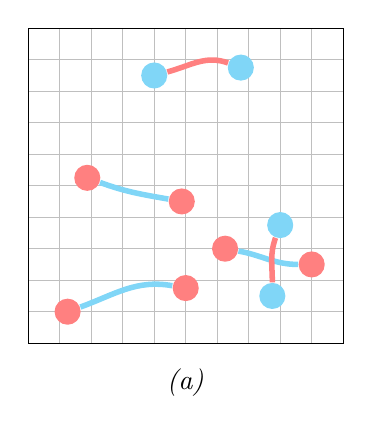
\begin{tikzpicture}
      \drawquasigrid
      \node at (2, -.5) {\emph{(a)}};
    \end{tikzpicture}
    \hspace{1cm}
    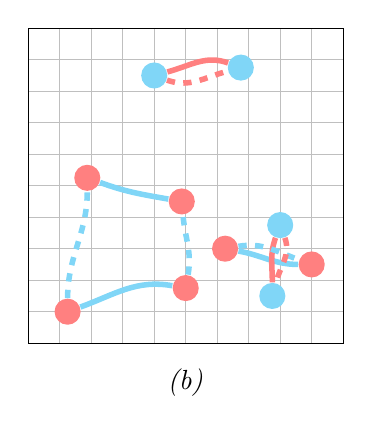
\begin{tikzpicture}
      \drawquasigrid
      \draw[dashed, blueline] (N1) to[out=90, in=270] (N5);
      \draw[dashed, blueline] (N2) to[out=80, in=275] (N6);
      \draw[dashed, blueline] (N3) to[out=10, in=160] (N4);
      \draw[dashed, redline] (N7) to[out=-20, in=195] (N8);
      \draw[dashed, redline] (N9) to[out=290, in=75] (N10);
      \node at (2, -.5) {\emph{(b)}};
    \end{tikzpicture}
    \hspace{1cm}
    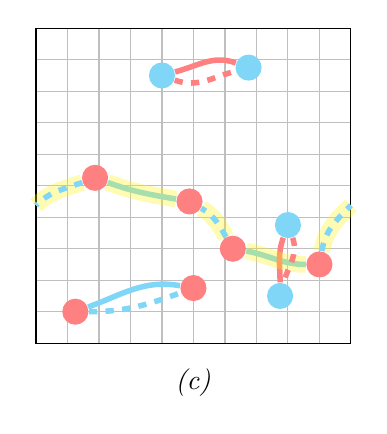
\begin{tikzpicture}
      \drawquasigrid
      \draw[yellow, line width=6, opacity=.3] (N3) to[in=180, out=-10] (N4);
      \draw[yellow, line width=6, opacity=.3] (N5) to[in=170, out=-20] (N6);
      \draw[yellow, line width=6, opacity=.3] (N3) to[out=120, in=-30] (N6);
      \draw[yellow, line width=6, opacity=.3] (N5) to[out=200, in=45] (0, 1.75);
      \draw[yellow, line width=6, opacity=.3] (N4) to[out=80, in=225] (4, 1.75);
      \draw[dashed, blueline] (N1) to[out=0, in=200] (N2);
      \draw[dashed, blueline] (N3) to[out=120, in=-30] (N6);
      \draw[dashed, blueline] (N5) to[out=200, in=45] (0, 1.75);
      \draw[dashed, blueline] (N4) to[out=80, in=225] (4, 1.75);
      \draw[dashed, redline] (N7) to[out=-20, in=195] (N8);
      \draw[dashed, redline] (N9) to[out=290, in=75] (N10);
      \node at (2, -.5) {\emph{(c)}};
    \end{tikzpicture}
    \caption{The quasiparticle picture of stabilizer measurements. Anticommuting stabilizers behave as anyons (circles), where a chain of errors (lines) creates a pair of anyons. Figure (b) shows a successful decoding of (a). Figure (c) shows a pairing that resulted in a correction operator that is in a different class as the error operator, which acquires a logical error. (Figure inspired by \cite{naomi})}\label{fig:quasiparticle}
  \end{figure}
  
Figure \ref{fig:quasiparticle}a shows the quasiparticle representation of the errors suffered in Figure \ref{sf:fig_degenerate}a, which has suffered Z (blue lines) and X errors (red lines). The corresponding anyons can either be of the star type (red circle) or plaquette type (blue circle). Figure \ref{fig:quasiparticle}b shows a successful decoding. Note that here not all pairs are correctly identified, but the resulting loop still is in the same class of operators. In Figure \ref{fig:quasiparticle}c the correction has failed as the resulting loop in the correction is in a difference class compared to the error. As the loop still commutes with the stabilizer, no error can be detected, but the encoded qubit has acquired a logical error.

\subsection{Performance}

\begin{figure}[ht]
  \centering
  \begin{subfigure}[b]{\textwidth}
    %% Creator: Matplotlib, PGF backend
%%
%% To include the figure in your LaTeX document, write
%%   \input{<filename>.pgf}
%%
%% Make sure the required packages are loaded in your preamble
%%   \usepackage{pgf}
%%
%% Figures using additional raster images can only be included by \input if
%% they are in the same directory as the main LaTeX file. For loading figures
%% from other directories you can use the `import` package
%%   \usepackage{import}
%% and then include the figures with
%%   \import{<path to file>}{<filename>.pgf}
%%
%% Matplotlib used the following preamble
%%   \usepackage[utf8x]{inputenc}
%%   \usepackage[T1]{fontenc}
%%
\begingroup%
\makeatletter%
\begin{pgfpicture}%
\pgfpathrectangle{\pgfpointorigin}{\pgfqpoint{5.400000in}{3.330000in}}%
\pgfusepath{use as bounding box, clip}%
\begin{pgfscope}%
\pgfsetbuttcap%
\pgfsetmiterjoin%
\definecolor{currentfill}{rgb}{1.000000,1.000000,1.000000}%
\pgfsetfillcolor{currentfill}%
\pgfsetlinewidth{0.000000pt}%
\definecolor{currentstroke}{rgb}{1.000000,1.000000,1.000000}%
\pgfsetstrokecolor{currentstroke}%
\pgfsetdash{}{0pt}%
\pgfpathmoveto{\pgfqpoint{0.000000in}{0.000000in}}%
\pgfpathlineto{\pgfqpoint{5.400000in}{0.000000in}}%
\pgfpathlineto{\pgfqpoint{5.400000in}{3.330000in}}%
\pgfpathlineto{\pgfqpoint{0.000000in}{3.330000in}}%
\pgfpathclose%
\pgfusepath{fill}%
\end{pgfscope}%
\begin{pgfscope}%
\pgfsetbuttcap%
\pgfsetmiterjoin%
\definecolor{currentfill}{rgb}{1.000000,1.000000,1.000000}%
\pgfsetfillcolor{currentfill}%
\pgfsetlinewidth{0.000000pt}%
\definecolor{currentstroke}{rgb}{0.000000,0.000000,0.000000}%
\pgfsetstrokecolor{currentstroke}%
\pgfsetstrokeopacity{0.000000}%
\pgfsetdash{}{0pt}%
\pgfpathmoveto{\pgfqpoint{0.693677in}{0.538351in}}%
\pgfpathlineto{\pgfqpoint{5.215000in}{0.538351in}}%
\pgfpathlineto{\pgfqpoint{5.215000in}{3.145409in}}%
\pgfpathlineto{\pgfqpoint{0.693677in}{3.145409in}}%
\pgfpathclose%
\pgfusepath{fill}%
\end{pgfscope}%
\begin{pgfscope}%
\pgfsetbuttcap%
\pgfsetroundjoin%
\definecolor{currentfill}{rgb}{0.000000,0.000000,0.000000}%
\pgfsetfillcolor{currentfill}%
\pgfsetlinewidth{0.803000pt}%
\definecolor{currentstroke}{rgb}{0.000000,0.000000,0.000000}%
\pgfsetstrokecolor{currentstroke}%
\pgfsetdash{}{0pt}%
\pgfsys@defobject{currentmarker}{\pgfqpoint{0.000000in}{-0.048611in}}{\pgfqpoint{0.000000in}{0.000000in}}{%
\pgfpathmoveto{\pgfqpoint{0.000000in}{0.000000in}}%
\pgfpathlineto{\pgfqpoint{0.000000in}{-0.048611in}}%
\pgfusepath{stroke,fill}%
}%
\begin{pgfscope}%
\pgfsys@transformshift{0.834968in}{0.538351in}%
\pgfsys@useobject{currentmarker}{}%
\end{pgfscope}%
\end{pgfscope}%
\begin{pgfscope}%
\pgftext[x=0.834968in,y=0.441128in,,top]{\rmfamily\fontsize{8.000000}{9.600000}\selectfont \(\displaystyle 10.0\)}%
\end{pgfscope}%
\begin{pgfscope}%
\pgfsetbuttcap%
\pgfsetroundjoin%
\definecolor{currentfill}{rgb}{0.000000,0.000000,0.000000}%
\pgfsetfillcolor{currentfill}%
\pgfsetlinewidth{0.803000pt}%
\definecolor{currentstroke}{rgb}{0.000000,0.000000,0.000000}%
\pgfsetstrokecolor{currentstroke}%
\pgfsetdash{}{0pt}%
\pgfsys@defobject{currentmarker}{\pgfqpoint{0.000000in}{-0.048611in}}{\pgfqpoint{0.000000in}{0.000000in}}{%
\pgfpathmoveto{\pgfqpoint{0.000000in}{0.000000in}}%
\pgfpathlineto{\pgfqpoint{0.000000in}{-0.048611in}}%
\pgfusepath{stroke,fill}%
}%
\begin{pgfscope}%
\pgfsys@transformshift{1.541425in}{0.538351in}%
\pgfsys@useobject{currentmarker}{}%
\end{pgfscope}%
\end{pgfscope}%
\begin{pgfscope}%
\pgftext[x=1.541425in,y=0.441128in,,top]{\rmfamily\fontsize{8.000000}{9.600000}\selectfont \(\displaystyle 10.1\)}%
\end{pgfscope}%
\begin{pgfscope}%
\pgfsetbuttcap%
\pgfsetroundjoin%
\definecolor{currentfill}{rgb}{0.000000,0.000000,0.000000}%
\pgfsetfillcolor{currentfill}%
\pgfsetlinewidth{0.803000pt}%
\definecolor{currentstroke}{rgb}{0.000000,0.000000,0.000000}%
\pgfsetstrokecolor{currentstroke}%
\pgfsetdash{}{0pt}%
\pgfsys@defobject{currentmarker}{\pgfqpoint{0.000000in}{-0.048611in}}{\pgfqpoint{0.000000in}{0.000000in}}{%
\pgfpathmoveto{\pgfqpoint{0.000000in}{0.000000in}}%
\pgfpathlineto{\pgfqpoint{0.000000in}{-0.048611in}}%
\pgfusepath{stroke,fill}%
}%
\begin{pgfscope}%
\pgfsys@transformshift{2.247882in}{0.538351in}%
\pgfsys@useobject{currentmarker}{}%
\end{pgfscope}%
\end{pgfscope}%
\begin{pgfscope}%
\pgftext[x=2.247882in,y=0.441128in,,top]{\rmfamily\fontsize{8.000000}{9.600000}\selectfont \(\displaystyle 10.2\)}%
\end{pgfscope}%
\begin{pgfscope}%
\pgfsetbuttcap%
\pgfsetroundjoin%
\definecolor{currentfill}{rgb}{0.000000,0.000000,0.000000}%
\pgfsetfillcolor{currentfill}%
\pgfsetlinewidth{0.803000pt}%
\definecolor{currentstroke}{rgb}{0.000000,0.000000,0.000000}%
\pgfsetstrokecolor{currentstroke}%
\pgfsetdash{}{0pt}%
\pgfsys@defobject{currentmarker}{\pgfqpoint{0.000000in}{-0.048611in}}{\pgfqpoint{0.000000in}{0.000000in}}{%
\pgfpathmoveto{\pgfqpoint{0.000000in}{0.000000in}}%
\pgfpathlineto{\pgfqpoint{0.000000in}{-0.048611in}}%
\pgfusepath{stroke,fill}%
}%
\begin{pgfscope}%
\pgfsys@transformshift{2.954338in}{0.538351in}%
\pgfsys@useobject{currentmarker}{}%
\end{pgfscope}%
\end{pgfscope}%
\begin{pgfscope}%
\pgftext[x=2.954338in,y=0.441128in,,top]{\rmfamily\fontsize{8.000000}{9.600000}\selectfont \(\displaystyle 10.3\)}%
\end{pgfscope}%
\begin{pgfscope}%
\pgfsetbuttcap%
\pgfsetroundjoin%
\definecolor{currentfill}{rgb}{0.000000,0.000000,0.000000}%
\pgfsetfillcolor{currentfill}%
\pgfsetlinewidth{0.803000pt}%
\definecolor{currentstroke}{rgb}{0.000000,0.000000,0.000000}%
\pgfsetstrokecolor{currentstroke}%
\pgfsetdash{}{0pt}%
\pgfsys@defobject{currentmarker}{\pgfqpoint{0.000000in}{-0.048611in}}{\pgfqpoint{0.000000in}{0.000000in}}{%
\pgfpathmoveto{\pgfqpoint{0.000000in}{0.000000in}}%
\pgfpathlineto{\pgfqpoint{0.000000in}{-0.048611in}}%
\pgfusepath{stroke,fill}%
}%
\begin{pgfscope}%
\pgfsys@transformshift{3.660795in}{0.538351in}%
\pgfsys@useobject{currentmarker}{}%
\end{pgfscope}%
\end{pgfscope}%
\begin{pgfscope}%
\pgftext[x=3.660795in,y=0.441128in,,top]{\rmfamily\fontsize{8.000000}{9.600000}\selectfont \(\displaystyle 10.4\)}%
\end{pgfscope}%
\begin{pgfscope}%
\pgfsetbuttcap%
\pgfsetroundjoin%
\definecolor{currentfill}{rgb}{0.000000,0.000000,0.000000}%
\pgfsetfillcolor{currentfill}%
\pgfsetlinewidth{0.803000pt}%
\definecolor{currentstroke}{rgb}{0.000000,0.000000,0.000000}%
\pgfsetstrokecolor{currentstroke}%
\pgfsetdash{}{0pt}%
\pgfsys@defobject{currentmarker}{\pgfqpoint{0.000000in}{-0.048611in}}{\pgfqpoint{0.000000in}{0.000000in}}{%
\pgfpathmoveto{\pgfqpoint{0.000000in}{0.000000in}}%
\pgfpathlineto{\pgfqpoint{0.000000in}{-0.048611in}}%
\pgfusepath{stroke,fill}%
}%
\begin{pgfscope}%
\pgfsys@transformshift{4.367252in}{0.538351in}%
\pgfsys@useobject{currentmarker}{}%
\end{pgfscope}%
\end{pgfscope}%
\begin{pgfscope}%
\pgftext[x=4.367252in,y=0.441128in,,top]{\rmfamily\fontsize{8.000000}{9.600000}\selectfont \(\displaystyle 10.5\)}%
\end{pgfscope}%
\begin{pgfscope}%
\pgfsetbuttcap%
\pgfsetroundjoin%
\definecolor{currentfill}{rgb}{0.000000,0.000000,0.000000}%
\pgfsetfillcolor{currentfill}%
\pgfsetlinewidth{0.803000pt}%
\definecolor{currentstroke}{rgb}{0.000000,0.000000,0.000000}%
\pgfsetstrokecolor{currentstroke}%
\pgfsetdash{}{0pt}%
\pgfsys@defobject{currentmarker}{\pgfqpoint{0.000000in}{-0.048611in}}{\pgfqpoint{0.000000in}{0.000000in}}{%
\pgfpathmoveto{\pgfqpoint{0.000000in}{0.000000in}}%
\pgfpathlineto{\pgfqpoint{0.000000in}{-0.048611in}}%
\pgfusepath{stroke,fill}%
}%
\begin{pgfscope}%
\pgfsys@transformshift{5.073709in}{0.538351in}%
\pgfsys@useobject{currentmarker}{}%
\end{pgfscope}%
\end{pgfscope}%
\begin{pgfscope}%
\pgftext[x=5.073709in,y=0.441128in,,top]{\rmfamily\fontsize{8.000000}{9.600000}\selectfont \(\displaystyle 10.6\)}%
\end{pgfscope}%
\begin{pgfscope}%
\pgftext[x=2.954338in,y=0.287449in,,top]{\rmfamily\fontsize{10.000000}{12.000000}\selectfont probability of Pauli X error (\%)}%
\end{pgfscope}%
\begin{pgfscope}%
\pgfsetbuttcap%
\pgfsetroundjoin%
\definecolor{currentfill}{rgb}{0.000000,0.000000,0.000000}%
\pgfsetfillcolor{currentfill}%
\pgfsetlinewidth{0.803000pt}%
\definecolor{currentstroke}{rgb}{0.000000,0.000000,0.000000}%
\pgfsetstrokecolor{currentstroke}%
\pgfsetdash{}{0pt}%
\pgfsys@defobject{currentmarker}{\pgfqpoint{-0.048611in}{0.000000in}}{\pgfqpoint{0.000000in}{0.000000in}}{%
\pgfpathmoveto{\pgfqpoint{0.000000in}{0.000000in}}%
\pgfpathlineto{\pgfqpoint{-0.048611in}{0.000000in}}%
\pgfusepath{stroke,fill}%
}%
\begin{pgfscope}%
\pgfsys@transformshift{0.693677in}{0.538351in}%
\pgfsys@useobject{currentmarker}{}%
\end{pgfscope}%
\end{pgfscope}%
\begin{pgfscope}%
\pgftext[x=0.386575in,y=0.500088in,left,base]{\rmfamily\fontsize{8.000000}{9.600000}\selectfont \(\displaystyle 0.60\)}%
\end{pgfscope}%
\begin{pgfscope}%
\pgfsetbuttcap%
\pgfsetroundjoin%
\definecolor{currentfill}{rgb}{0.000000,0.000000,0.000000}%
\pgfsetfillcolor{currentfill}%
\pgfsetlinewidth{0.803000pt}%
\definecolor{currentstroke}{rgb}{0.000000,0.000000,0.000000}%
\pgfsetstrokecolor{currentstroke}%
\pgfsetdash{}{0pt}%
\pgfsys@defobject{currentmarker}{\pgfqpoint{-0.048611in}{0.000000in}}{\pgfqpoint{0.000000in}{0.000000in}}{%
\pgfpathmoveto{\pgfqpoint{0.000000in}{0.000000in}}%
\pgfpathlineto{\pgfqpoint{-0.048611in}{0.000000in}}%
\pgfusepath{stroke,fill}%
}%
\begin{pgfscope}%
\pgfsys@transformshift{0.693677in}{1.059762in}%
\pgfsys@useobject{currentmarker}{}%
\end{pgfscope}%
\end{pgfscope}%
\begin{pgfscope}%
\pgftext[x=0.386575in,y=1.021500in,left,base]{\rmfamily\fontsize{8.000000}{9.600000}\selectfont \(\displaystyle 0.65\)}%
\end{pgfscope}%
\begin{pgfscope}%
\pgfsetbuttcap%
\pgfsetroundjoin%
\definecolor{currentfill}{rgb}{0.000000,0.000000,0.000000}%
\pgfsetfillcolor{currentfill}%
\pgfsetlinewidth{0.803000pt}%
\definecolor{currentstroke}{rgb}{0.000000,0.000000,0.000000}%
\pgfsetstrokecolor{currentstroke}%
\pgfsetdash{}{0pt}%
\pgfsys@defobject{currentmarker}{\pgfqpoint{-0.048611in}{0.000000in}}{\pgfqpoint{0.000000in}{0.000000in}}{%
\pgfpathmoveto{\pgfqpoint{0.000000in}{0.000000in}}%
\pgfpathlineto{\pgfqpoint{-0.048611in}{0.000000in}}%
\pgfusepath{stroke,fill}%
}%
\begin{pgfscope}%
\pgfsys@transformshift{0.693677in}{1.581174in}%
\pgfsys@useobject{currentmarker}{}%
\end{pgfscope}%
\end{pgfscope}%
\begin{pgfscope}%
\pgftext[x=0.386575in,y=1.542912in,left,base]{\rmfamily\fontsize{8.000000}{9.600000}\selectfont \(\displaystyle 0.70\)}%
\end{pgfscope}%
\begin{pgfscope}%
\pgfsetbuttcap%
\pgfsetroundjoin%
\definecolor{currentfill}{rgb}{0.000000,0.000000,0.000000}%
\pgfsetfillcolor{currentfill}%
\pgfsetlinewidth{0.803000pt}%
\definecolor{currentstroke}{rgb}{0.000000,0.000000,0.000000}%
\pgfsetstrokecolor{currentstroke}%
\pgfsetdash{}{0pt}%
\pgfsys@defobject{currentmarker}{\pgfqpoint{-0.048611in}{0.000000in}}{\pgfqpoint{0.000000in}{0.000000in}}{%
\pgfpathmoveto{\pgfqpoint{0.000000in}{0.000000in}}%
\pgfpathlineto{\pgfqpoint{-0.048611in}{0.000000in}}%
\pgfusepath{stroke,fill}%
}%
\begin{pgfscope}%
\pgfsys@transformshift{0.693677in}{2.102586in}%
\pgfsys@useobject{currentmarker}{}%
\end{pgfscope}%
\end{pgfscope}%
\begin{pgfscope}%
\pgftext[x=0.386575in,y=2.064324in,left,base]{\rmfamily\fontsize{8.000000}{9.600000}\selectfont \(\displaystyle 0.75\)}%
\end{pgfscope}%
\begin{pgfscope}%
\pgfsetbuttcap%
\pgfsetroundjoin%
\definecolor{currentfill}{rgb}{0.000000,0.000000,0.000000}%
\pgfsetfillcolor{currentfill}%
\pgfsetlinewidth{0.803000pt}%
\definecolor{currentstroke}{rgb}{0.000000,0.000000,0.000000}%
\pgfsetstrokecolor{currentstroke}%
\pgfsetdash{}{0pt}%
\pgfsys@defobject{currentmarker}{\pgfqpoint{-0.048611in}{0.000000in}}{\pgfqpoint{0.000000in}{0.000000in}}{%
\pgfpathmoveto{\pgfqpoint{0.000000in}{0.000000in}}%
\pgfpathlineto{\pgfqpoint{-0.048611in}{0.000000in}}%
\pgfusepath{stroke,fill}%
}%
\begin{pgfscope}%
\pgfsys@transformshift{0.693677in}{2.623998in}%
\pgfsys@useobject{currentmarker}{}%
\end{pgfscope}%
\end{pgfscope}%
\begin{pgfscope}%
\pgftext[x=0.386575in,y=2.585735in,left,base]{\rmfamily\fontsize{8.000000}{9.600000}\selectfont \(\displaystyle 0.80\)}%
\end{pgfscope}%
\begin{pgfscope}%
\pgfsetbuttcap%
\pgfsetroundjoin%
\definecolor{currentfill}{rgb}{0.000000,0.000000,0.000000}%
\pgfsetfillcolor{currentfill}%
\pgfsetlinewidth{0.803000pt}%
\definecolor{currentstroke}{rgb}{0.000000,0.000000,0.000000}%
\pgfsetstrokecolor{currentstroke}%
\pgfsetdash{}{0pt}%
\pgfsys@defobject{currentmarker}{\pgfqpoint{-0.048611in}{0.000000in}}{\pgfqpoint{0.000000in}{0.000000in}}{%
\pgfpathmoveto{\pgfqpoint{0.000000in}{0.000000in}}%
\pgfpathlineto{\pgfqpoint{-0.048611in}{0.000000in}}%
\pgfusepath{stroke,fill}%
}%
\begin{pgfscope}%
\pgfsys@transformshift{0.693677in}{3.145409in}%
\pgfsys@useobject{currentmarker}{}%
\end{pgfscope}%
\end{pgfscope}%
\begin{pgfscope}%
\pgftext[x=0.386575in,y=3.107147in,left,base]{\rmfamily\fontsize{8.000000}{9.600000}\selectfont \(\displaystyle 0.85\)}%
\end{pgfscope}%
\begin{pgfscope}%
\pgftext[x=0.331019in,y=1.841880in,,bottom,rotate=90.000000]{\rmfamily\fontsize{10.000000}{12.000000}\selectfont decoding success rate}%
\end{pgfscope}%
\begin{pgfscope}%
\pgfpathrectangle{\pgfqpoint{0.693677in}{0.538351in}}{\pgfqpoint{4.521323in}{2.607059in}} %
\pgfusepath{clip}%
\pgfsetbuttcap%
\pgfsetroundjoin%
\definecolor{currentfill}{rgb}{0.172549,0.627451,0.172549}%
\pgfsetfillcolor{currentfill}%
\pgfsetlinewidth{1.003750pt}%
\definecolor{currentstroke}{rgb}{0.172549,0.627451,0.172549}%
\pgfsetstrokecolor{currentstroke}%
\pgfsetdash{}{0pt}%
\pgfsys@defobject{currentmarker}{\pgfqpoint{-0.017361in}{-0.017361in}}{\pgfqpoint{0.017361in}{0.017361in}}{%
\pgfpathmoveto{\pgfqpoint{0.000000in}{-0.017361in}}%
\pgfpathcurveto{\pgfqpoint{0.004604in}{-0.017361in}}{\pgfqpoint{0.009020in}{-0.015532in}}{\pgfqpoint{0.012276in}{-0.012276in}}%
\pgfpathcurveto{\pgfqpoint{0.015532in}{-0.009020in}}{\pgfqpoint{0.017361in}{-0.004604in}}{\pgfqpoint{0.017361in}{0.000000in}}%
\pgfpathcurveto{\pgfqpoint{0.017361in}{0.004604in}}{\pgfqpoint{0.015532in}{0.009020in}}{\pgfqpoint{0.012276in}{0.012276in}}%
\pgfpathcurveto{\pgfqpoint{0.009020in}{0.015532in}}{\pgfqpoint{0.004604in}{0.017361in}}{\pgfqpoint{0.000000in}{0.017361in}}%
\pgfpathcurveto{\pgfqpoint{-0.004604in}{0.017361in}}{\pgfqpoint{-0.009020in}{0.015532in}}{\pgfqpoint{-0.012276in}{0.012276in}}%
\pgfpathcurveto{\pgfqpoint{-0.015532in}{0.009020in}}{\pgfqpoint{-0.017361in}{0.004604in}}{\pgfqpoint{-0.017361in}{0.000000in}}%
\pgfpathcurveto{\pgfqpoint{-0.017361in}{-0.004604in}}{\pgfqpoint{-0.015532in}{-0.009020in}}{\pgfqpoint{-0.012276in}{-0.012276in}}%
\pgfpathcurveto{\pgfqpoint{-0.009020in}{-0.015532in}}{\pgfqpoint{-0.004604in}{-0.017361in}}{\pgfqpoint{0.000000in}{-0.017361in}}%
\pgfpathclose%
\pgfusepath{stroke,fill}%
}%
\begin{pgfscope}%
\pgfsys@transformshift{0.834968in}{1.950885in}%
\pgfsys@useobject{currentmarker}{}%
\end{pgfscope}%
\begin{pgfscope}%
\pgfsys@transformshift{1.188197in}{1.945372in}%
\pgfsys@useobject{currentmarker}{}%
\end{pgfscope}%
\begin{pgfscope}%
\pgfsys@transformshift{1.541425in}{1.936682in}%
\pgfsys@useobject{currentmarker}{}%
\end{pgfscope}%
\begin{pgfscope}%
\pgfsys@transformshift{1.894653in}{1.872888in}%
\pgfsys@useobject{currentmarker}{}%
\end{pgfscope}%
\begin{pgfscope}%
\pgfsys@transformshift{2.247882in}{1.866766in}%
\pgfsys@useobject{currentmarker}{}%
\end{pgfscope}%
\begin{pgfscope}%
\pgfsys@transformshift{2.601110in}{1.829042in}%
\pgfsys@useobject{currentmarker}{}%
\end{pgfscope}%
\begin{pgfscope}%
\pgfsys@transformshift{2.954338in}{1.773492in}%
\pgfsys@useobject{currentmarker}{}%
\end{pgfscope}%
\begin{pgfscope}%
\pgfsys@transformshift{3.307567in}{1.736215in}%
\pgfsys@useobject{currentmarker}{}%
\end{pgfscope}%
\begin{pgfscope}%
\pgfsys@transformshift{3.660795in}{1.690394in}%
\pgfsys@useobject{currentmarker}{}%
\end{pgfscope}%
\begin{pgfscope}%
\pgfsys@transformshift{4.014024in}{1.651881in}%
\pgfsys@useobject{currentmarker}{}%
\end{pgfscope}%
\begin{pgfscope}%
\pgfsys@transformshift{4.367252in}{1.598357in}%
\pgfsys@useobject{currentmarker}{}%
\end{pgfscope}%
\begin{pgfscope}%
\pgfsys@transformshift{4.720480in}{1.542266in}%
\pgfsys@useobject{currentmarker}{}%
\end{pgfscope}%
\begin{pgfscope}%
\pgfsys@transformshift{5.073709in}{1.561905in}%
\pgfsys@useobject{currentmarker}{}%
\end{pgfscope}%
\end{pgfscope}%
\begin{pgfscope}%
\pgfpathrectangle{\pgfqpoint{0.693677in}{0.538351in}}{\pgfqpoint{4.521323in}{2.607059in}} %
\pgfusepath{clip}%
\pgfsetrectcap%
\pgfsetroundjoin%
\pgfsetlinewidth{1.505625pt}%
\definecolor{currentstroke}{rgb}{0.172549,0.627451,0.172549}%
\pgfsetstrokecolor{currentstroke}%
\pgfsetstrokeopacity{0.600000}%
\pgfsetdash{}{0pt}%
\pgfpathmoveto{\pgfqpoint{0.834968in}{1.999875in}}%
\pgfpathlineto{\pgfqpoint{2.154536in}{1.861166in}}%
\pgfpathlineto{\pgfqpoint{3.474104in}{1.720226in}}%
\pgfpathlineto{\pgfqpoint{4.793672in}{1.577055in}}%
\pgfpathlineto{\pgfqpoint{5.073709in}{1.546385in}}%
\pgfpathlineto{\pgfqpoint{5.073709in}{1.546385in}}%
\pgfusepath{stroke}%
\end{pgfscope}%
\begin{pgfscope}%
\pgfpathrectangle{\pgfqpoint{0.693677in}{0.538351in}}{\pgfqpoint{4.521323in}{2.607059in}} %
\pgfusepath{clip}%
\pgfsetbuttcap%
\pgfsetroundjoin%
\definecolor{currentfill}{rgb}{0.580392,0.403922,0.741176}%
\pgfsetfillcolor{currentfill}%
\pgfsetlinewidth{1.003750pt}%
\definecolor{currentstroke}{rgb}{0.580392,0.403922,0.741176}%
\pgfsetstrokecolor{currentstroke}%
\pgfsetdash{}{0pt}%
\pgfsys@defobject{currentmarker}{\pgfqpoint{-0.017361in}{-0.017361in}}{\pgfqpoint{0.017361in}{0.017361in}}{%
\pgfpathmoveto{\pgfqpoint{0.000000in}{-0.017361in}}%
\pgfpathcurveto{\pgfqpoint{0.004604in}{-0.017361in}}{\pgfqpoint{0.009020in}{-0.015532in}}{\pgfqpoint{0.012276in}{-0.012276in}}%
\pgfpathcurveto{\pgfqpoint{0.015532in}{-0.009020in}}{\pgfqpoint{0.017361in}{-0.004604in}}{\pgfqpoint{0.017361in}{0.000000in}}%
\pgfpathcurveto{\pgfqpoint{0.017361in}{0.004604in}}{\pgfqpoint{0.015532in}{0.009020in}}{\pgfqpoint{0.012276in}{0.012276in}}%
\pgfpathcurveto{\pgfqpoint{0.009020in}{0.015532in}}{\pgfqpoint{0.004604in}{0.017361in}}{\pgfqpoint{0.000000in}{0.017361in}}%
\pgfpathcurveto{\pgfqpoint{-0.004604in}{0.017361in}}{\pgfqpoint{-0.009020in}{0.015532in}}{\pgfqpoint{-0.012276in}{0.012276in}}%
\pgfpathcurveto{\pgfqpoint{-0.015532in}{0.009020in}}{\pgfqpoint{-0.017361in}{0.004604in}}{\pgfqpoint{-0.017361in}{0.000000in}}%
\pgfpathcurveto{\pgfqpoint{-0.017361in}{-0.004604in}}{\pgfqpoint{-0.015532in}{-0.009020in}}{\pgfqpoint{-0.012276in}{-0.012276in}}%
\pgfpathcurveto{\pgfqpoint{-0.009020in}{-0.015532in}}{\pgfqpoint{-0.004604in}{-0.017361in}}{\pgfqpoint{0.000000in}{-0.017361in}}%
\pgfpathclose%
\pgfusepath{stroke,fill}%
}%
\begin{pgfscope}%
\pgfsys@transformshift{0.834968in}{2.141889in}%
\pgfsys@useobject{currentmarker}{}%
\end{pgfscope}%
\begin{pgfscope}%
\pgfsys@transformshift{1.188197in}{2.096858in}%
\pgfsys@useobject{currentmarker}{}%
\end{pgfscope}%
\begin{pgfscope}%
\pgfsys@transformshift{1.541425in}{2.066245in}%
\pgfsys@useobject{currentmarker}{}%
\end{pgfscope}%
\begin{pgfscope}%
\pgfsys@transformshift{1.894653in}{1.984873in}%
\pgfsys@useobject{currentmarker}{}%
\end{pgfscope}%
\begin{pgfscope}%
\pgfsys@transformshift{2.247882in}{1.901329in}%
\pgfsys@useobject{currentmarker}{}%
\end{pgfscope}%
\begin{pgfscope}%
\pgfsys@transformshift{2.601110in}{1.868346in}%
\pgfsys@useobject{currentmarker}{}%
\end{pgfscope}%
\begin{pgfscope}%
\pgfsys@transformshift{2.954338in}{1.834572in}%
\pgfsys@useobject{currentmarker}{}%
\end{pgfscope}%
\begin{pgfscope}%
\pgfsys@transformshift{3.307567in}{1.744905in}%
\pgfsys@useobject{currentmarker}{}%
\end{pgfscope}%
\begin{pgfscope}%
\pgfsys@transformshift{3.660795in}{1.676766in}%
\pgfsys@useobject{currentmarker}{}%
\end{pgfscope}%
\begin{pgfscope}%
\pgfsys@transformshift{4.014024in}{1.576631in}%
\pgfsys@useobject{currentmarker}{}%
\end{pgfscope}%
\begin{pgfscope}%
\pgfsys@transformshift{4.367252in}{1.539896in}%
\pgfsys@useobject{currentmarker}{}%
\end{pgfscope}%
\begin{pgfscope}%
\pgfsys@transformshift{4.720480in}{1.491310in}%
\pgfsys@useobject{currentmarker}{}%
\end{pgfscope}%
\begin{pgfscope}%
\pgfsys@transformshift{5.073709in}{1.473732in}%
\pgfsys@useobject{currentmarker}{}%
\end{pgfscope}%
\end{pgfscope}%
\begin{pgfscope}%
\pgfpathrectangle{\pgfqpoint{0.693677in}{0.538351in}}{\pgfqpoint{4.521323in}{2.607059in}} %
\pgfusepath{clip}%
\pgfsetrectcap%
\pgfsetroundjoin%
\pgfsetlinewidth{1.505625pt}%
\definecolor{currentstroke}{rgb}{0.580392,0.403922,0.741176}%
\pgfsetstrokecolor{currentstroke}%
\pgfsetstrokeopacity{0.600000}%
\pgfsetdash{}{0pt}%
\pgfpathmoveto{\pgfqpoint{0.834968in}{2.158814in}}%
\pgfpathlineto{\pgfqpoint{1.653864in}{2.021811in}}%
\pgfpathlineto{\pgfqpoint{2.472760in}{1.882548in}}%
\pgfpathlineto{\pgfqpoint{3.291656in}{1.741024in}}%
\pgfpathlineto{\pgfqpoint{4.110551in}{1.597240in}}%
\pgfpathlineto{\pgfqpoint{4.929447in}{1.451195in}}%
\pgfpathlineto{\pgfqpoint{5.073709in}{1.425233in}}%
\pgfpathlineto{\pgfqpoint{5.073709in}{1.425233in}}%
\pgfusepath{stroke}%
\end{pgfscope}%
\begin{pgfscope}%
\pgfpathrectangle{\pgfqpoint{0.693677in}{0.538351in}}{\pgfqpoint{4.521323in}{2.607059in}} %
\pgfusepath{clip}%
\pgfsetbuttcap%
\pgfsetroundjoin%
\definecolor{currentfill}{rgb}{0.890196,0.466667,0.760784}%
\pgfsetfillcolor{currentfill}%
\pgfsetlinewidth{1.003750pt}%
\definecolor{currentstroke}{rgb}{0.890196,0.466667,0.760784}%
\pgfsetstrokecolor{currentstroke}%
\pgfsetdash{}{0pt}%
\pgfsys@defobject{currentmarker}{\pgfqpoint{-0.017361in}{-0.017361in}}{\pgfqpoint{0.017361in}{0.017361in}}{%
\pgfpathmoveto{\pgfqpoint{0.000000in}{-0.017361in}}%
\pgfpathcurveto{\pgfqpoint{0.004604in}{-0.017361in}}{\pgfqpoint{0.009020in}{-0.015532in}}{\pgfqpoint{0.012276in}{-0.012276in}}%
\pgfpathcurveto{\pgfqpoint{0.015532in}{-0.009020in}}{\pgfqpoint{0.017361in}{-0.004604in}}{\pgfqpoint{0.017361in}{0.000000in}}%
\pgfpathcurveto{\pgfqpoint{0.017361in}{0.004604in}}{\pgfqpoint{0.015532in}{0.009020in}}{\pgfqpoint{0.012276in}{0.012276in}}%
\pgfpathcurveto{\pgfqpoint{0.009020in}{0.015532in}}{\pgfqpoint{0.004604in}{0.017361in}}{\pgfqpoint{0.000000in}{0.017361in}}%
\pgfpathcurveto{\pgfqpoint{-0.004604in}{0.017361in}}{\pgfqpoint{-0.009020in}{0.015532in}}{\pgfqpoint{-0.012276in}{0.012276in}}%
\pgfpathcurveto{\pgfqpoint{-0.015532in}{0.009020in}}{\pgfqpoint{-0.017361in}{0.004604in}}{\pgfqpoint{-0.017361in}{0.000000in}}%
\pgfpathcurveto{\pgfqpoint{-0.017361in}{-0.004604in}}{\pgfqpoint{-0.015532in}{-0.009020in}}{\pgfqpoint{-0.012276in}{-0.012276in}}%
\pgfpathcurveto{\pgfqpoint{-0.009020in}{-0.015532in}}{\pgfqpoint{-0.004604in}{-0.017361in}}{\pgfqpoint{0.000000in}{-0.017361in}}%
\pgfpathclose%
\pgfusepath{stroke,fill}%
}%
\begin{pgfscope}%
\pgfsys@transformshift{0.834968in}{2.274612in}%
\pgfsys@useobject{currentmarker}{}%
\end{pgfscope}%
\begin{pgfscope}%
\pgfsys@transformshift{1.188197in}{2.221286in}%
\pgfsys@useobject{currentmarker}{}%
\end{pgfscope}%
\begin{pgfscope}%
\pgfsys@transformshift{1.541425in}{2.141889in}%
\pgfsys@useobject{currentmarker}{}%
\end{pgfscope}%
\begin{pgfscope}%
\pgfsys@transformshift{1.894653in}{2.078688in}%
\pgfsys@useobject{currentmarker}{}%
\end{pgfscope}%
\begin{pgfscope}%
\pgfsys@transformshift{2.247882in}{1.961765in}%
\pgfsys@useobject{currentmarker}{}%
\end{pgfscope}%
\begin{pgfscope}%
\pgfsys@transformshift{2.601110in}{1.916734in}%
\pgfsys@useobject{currentmarker}{}%
\end{pgfscope}%
\begin{pgfscope}%
\pgfsys@transformshift{2.954338in}{1.825290in}%
\pgfsys@useobject{currentmarker}{}%
\end{pgfscope}%
\begin{pgfscope}%
\pgfsys@transformshift{3.307567in}{1.741745in}%
\pgfsys@useobject{currentmarker}{}%
\end{pgfscope}%
\begin{pgfscope}%
\pgfsys@transformshift{3.660795in}{1.679334in}%
\pgfsys@useobject{currentmarker}{}%
\end{pgfscope}%
\begin{pgfscope}%
\pgfsys@transformshift{4.014024in}{1.570706in}%
\pgfsys@useobject{currentmarker}{}%
\end{pgfscope}%
\begin{pgfscope}%
\pgfsys@transformshift{4.367252in}{1.483607in}%
\pgfsys@useobject{currentmarker}{}%
\end{pgfscope}%
\begin{pgfscope}%
\pgfsys@transformshift{4.720480in}{1.414085in}%
\pgfsys@useobject{currentmarker}{}%
\end{pgfscope}%
\begin{pgfscope}%
\pgfsys@transformshift{5.073709in}{1.352069in}%
\pgfsys@useobject{currentmarker}{}%
\end{pgfscope}%
\end{pgfscope}%
\begin{pgfscope}%
\pgfpathrectangle{\pgfqpoint{0.693677in}{0.538351in}}{\pgfqpoint{4.521323in}{2.607059in}} %
\pgfusepath{clip}%
\pgfsetrectcap%
\pgfsetroundjoin%
\pgfsetlinewidth{1.505625pt}%
\definecolor{currentstroke}{rgb}{0.890196,0.466667,0.760784}%
\pgfsetstrokecolor{currentstroke}%
\pgfsetstrokeopacity{0.600000}%
\pgfsetdash{}{0pt}%
\pgfpathmoveto{\pgfqpoint{0.834968in}{2.291945in}}%
\pgfpathlineto{\pgfqpoint{1.454444in}{2.156656in}}%
\pgfpathlineto{\pgfqpoint{2.073919in}{2.019090in}}%
\pgfpathlineto{\pgfqpoint{2.693395in}{1.879245in}}%
\pgfpathlineto{\pgfqpoint{3.312871in}{1.737123in}}%
\pgfpathlineto{\pgfqpoint{3.932346in}{1.592724in}}%
\pgfpathlineto{\pgfqpoint{4.551822in}{1.446047in}}%
\pgfpathlineto{\pgfqpoint{5.073709in}{1.320709in}}%
\pgfpathlineto{\pgfqpoint{5.073709in}{1.320709in}}%
\pgfusepath{stroke}%
\end{pgfscope}%
\begin{pgfscope}%
\pgfpathrectangle{\pgfqpoint{0.693677in}{0.538351in}}{\pgfqpoint{4.521323in}{2.607059in}} %
\pgfusepath{clip}%
\pgfsetbuttcap%
\pgfsetroundjoin%
\definecolor{currentfill}{rgb}{0.121569,0.466667,0.705882}%
\pgfsetfillcolor{currentfill}%
\pgfsetlinewidth{1.003750pt}%
\definecolor{currentstroke}{rgb}{0.121569,0.466667,0.705882}%
\pgfsetstrokecolor{currentstroke}%
\pgfsetdash{}{0pt}%
\pgfsys@defobject{currentmarker}{\pgfqpoint{-0.017361in}{-0.017361in}}{\pgfqpoint{0.017361in}{0.017361in}}{%
\pgfpathmoveto{\pgfqpoint{0.000000in}{-0.017361in}}%
\pgfpathcurveto{\pgfqpoint{0.004604in}{-0.017361in}}{\pgfqpoint{0.009020in}{-0.015532in}}{\pgfqpoint{0.012276in}{-0.012276in}}%
\pgfpathcurveto{\pgfqpoint{0.015532in}{-0.009020in}}{\pgfqpoint{0.017361in}{-0.004604in}}{\pgfqpoint{0.017361in}{0.000000in}}%
\pgfpathcurveto{\pgfqpoint{0.017361in}{0.004604in}}{\pgfqpoint{0.015532in}{0.009020in}}{\pgfqpoint{0.012276in}{0.012276in}}%
\pgfpathcurveto{\pgfqpoint{0.009020in}{0.015532in}}{\pgfqpoint{0.004604in}{0.017361in}}{\pgfqpoint{0.000000in}{0.017361in}}%
\pgfpathcurveto{\pgfqpoint{-0.004604in}{0.017361in}}{\pgfqpoint{-0.009020in}{0.015532in}}{\pgfqpoint{-0.012276in}{0.012276in}}%
\pgfpathcurveto{\pgfqpoint{-0.015532in}{0.009020in}}{\pgfqpoint{-0.017361in}{0.004604in}}{\pgfqpoint{-0.017361in}{0.000000in}}%
\pgfpathcurveto{\pgfqpoint{-0.017361in}{-0.004604in}}{\pgfqpoint{-0.015532in}{-0.009020in}}{\pgfqpoint{-0.012276in}{-0.012276in}}%
\pgfpathcurveto{\pgfqpoint{-0.009020in}{-0.015532in}}{\pgfqpoint{-0.004604in}{-0.017361in}}{\pgfqpoint{0.000000in}{-0.017361in}}%
\pgfpathclose%
\pgfusepath{stroke,fill}%
}%
\begin{pgfscope}%
\pgfsys@transformshift{0.834968in}{2.422346in}%
\pgfsys@useobject{currentmarker}{}%
\end{pgfscope}%
\begin{pgfscope}%
\pgfsys@transformshift{1.188197in}{2.355392in}%
\pgfsys@useobject{currentmarker}{}%
\end{pgfscope}%
\begin{pgfscope}%
\pgfsys@transformshift{1.541425in}{2.230766in}%
\pgfsys@useobject{currentmarker}{}%
\end{pgfscope}%
\begin{pgfscope}%
\pgfsys@transformshift{1.894653in}{2.130039in}%
\pgfsys@useobject{currentmarker}{}%
\end{pgfscope}%
\begin{pgfscope}%
\pgfsys@transformshift{2.247882in}{2.064665in}%
\pgfsys@useobject{currentmarker}{}%
\end{pgfscope}%
\begin{pgfscope}%
\pgfsys@transformshift{2.601110in}{1.925622in}%
\pgfsys@useobject{currentmarker}{}%
\end{pgfscope}%
\begin{pgfscope}%
\pgfsys@transformshift{2.954338in}{1.833782in}%
\pgfsys@useobject{currentmarker}{}%
\end{pgfscope}%
\begin{pgfscope}%
\pgfsys@transformshift{3.307567in}{1.721205in}%
\pgfsys@useobject{currentmarker}{}%
\end{pgfscope}%
\begin{pgfscope}%
\pgfsys@transformshift{3.660795in}{1.631143in}%
\pgfsys@useobject{currentmarker}{}%
\end{pgfscope}%
\begin{pgfscope}%
\pgfsys@transformshift{4.014024in}{1.522910in}%
\pgfsys@useobject{currentmarker}{}%
\end{pgfscope}%
\begin{pgfscope}%
\pgfsys@transformshift{4.367252in}{1.427121in}%
\pgfsys@useobject{currentmarker}{}%
\end{pgfscope}%
\begin{pgfscope}%
\pgfsys@transformshift{4.720480in}{1.276622in}%
\pgfsys@useobject{currentmarker}{}%
\end{pgfscope}%
\begin{pgfscope}%
\pgfsys@transformshift{5.073709in}{1.249959in}%
\pgfsys@useobject{currentmarker}{}%
\end{pgfscope}%
\end{pgfscope}%
\begin{pgfscope}%
\pgfpathrectangle{\pgfqpoint{0.693677in}{0.538351in}}{\pgfqpoint{4.521323in}{2.607059in}} %
\pgfusepath{clip}%
\pgfsetrectcap%
\pgfsetroundjoin%
\pgfsetlinewidth{1.505625pt}%
\definecolor{currentstroke}{rgb}{0.121569,0.466667,0.705882}%
\pgfsetstrokecolor{currentstroke}%
\pgfsetstrokeopacity{0.600000}%
\pgfsetdash{}{0pt}%
\pgfpathmoveto{\pgfqpoint{0.834968in}{2.410150in}}%
\pgfpathlineto{\pgfqpoint{1.344126in}{2.276263in}}%
\pgfpathlineto{\pgfqpoint{1.853284in}{2.140078in}}%
\pgfpathlineto{\pgfqpoint{2.362442in}{2.001594in}}%
\pgfpathlineto{\pgfqpoint{2.871600in}{1.860811in}}%
\pgfpathlineto{\pgfqpoint{3.380758in}{1.717729in}}%
\pgfpathlineto{\pgfqpoint{3.889916in}{1.572349in}}%
\pgfpathlineto{\pgfqpoint{4.399074in}{1.424670in}}%
\pgfpathlineto{\pgfqpoint{4.908232in}{1.274692in}}%
\pgfpathlineto{\pgfqpoint{5.073709in}{1.225455in}}%
\pgfpathlineto{\pgfqpoint{5.073709in}{1.225455in}}%
\pgfusepath{stroke}%
\end{pgfscope}%
\begin{pgfscope}%
\pgfpathrectangle{\pgfqpoint{0.693677in}{0.538351in}}{\pgfqpoint{4.521323in}{2.607059in}} %
\pgfusepath{clip}%
\pgfsetbuttcap%
\pgfsetroundjoin%
\definecolor{currentfill}{rgb}{0.839216,0.152941,0.156863}%
\pgfsetfillcolor{currentfill}%
\pgfsetlinewidth{1.003750pt}%
\definecolor{currentstroke}{rgb}{0.839216,0.152941,0.156863}%
\pgfsetstrokecolor{currentstroke}%
\pgfsetdash{}{0pt}%
\pgfsys@defobject{currentmarker}{\pgfqpoint{-0.017361in}{-0.017361in}}{\pgfqpoint{0.017361in}{0.017361in}}{%
\pgfpathmoveto{\pgfqpoint{0.000000in}{-0.017361in}}%
\pgfpathcurveto{\pgfqpoint{0.004604in}{-0.017361in}}{\pgfqpoint{0.009020in}{-0.015532in}}{\pgfqpoint{0.012276in}{-0.012276in}}%
\pgfpathcurveto{\pgfqpoint{0.015532in}{-0.009020in}}{\pgfqpoint{0.017361in}{-0.004604in}}{\pgfqpoint{0.017361in}{0.000000in}}%
\pgfpathcurveto{\pgfqpoint{0.017361in}{0.004604in}}{\pgfqpoint{0.015532in}{0.009020in}}{\pgfqpoint{0.012276in}{0.012276in}}%
\pgfpathcurveto{\pgfqpoint{0.009020in}{0.015532in}}{\pgfqpoint{0.004604in}{0.017361in}}{\pgfqpoint{0.000000in}{0.017361in}}%
\pgfpathcurveto{\pgfqpoint{-0.004604in}{0.017361in}}{\pgfqpoint{-0.009020in}{0.015532in}}{\pgfqpoint{-0.012276in}{0.012276in}}%
\pgfpathcurveto{\pgfqpoint{-0.015532in}{0.009020in}}{\pgfqpoint{-0.017361in}{0.004604in}}{\pgfqpoint{-0.017361in}{0.000000in}}%
\pgfpathcurveto{\pgfqpoint{-0.017361in}{-0.004604in}}{\pgfqpoint{-0.015532in}{-0.009020in}}{\pgfqpoint{-0.012276in}{-0.012276in}}%
\pgfpathcurveto{\pgfqpoint{-0.009020in}{-0.015532in}}{\pgfqpoint{-0.004604in}{-0.017361in}}{\pgfqpoint{0.000000in}{-0.017361in}}%
\pgfpathclose%
\pgfusepath{stroke,fill}%
}%
\begin{pgfscope}%
\pgfsys@transformshift{0.834968in}{2.532948in}%
\pgfsys@useobject{currentmarker}{}%
\end{pgfscope}%
\begin{pgfscope}%
\pgfsys@transformshift{1.188197in}{2.415235in}%
\pgfsys@useobject{currentmarker}{}%
\end{pgfscope}%
\begin{pgfscope}%
\pgfsys@transformshift{1.541425in}{2.303053in}%
\pgfsys@useobject{currentmarker}{}%
\end{pgfscope}%
\begin{pgfscope}%
\pgfsys@transformshift{1.894653in}{2.204893in}%
\pgfsys@useobject{currentmarker}{}%
\end{pgfscope}%
\begin{pgfscope}%
\pgfsys@transformshift{2.247882in}{2.102586in}%
\pgfsys@useobject{currentmarker}{}%
\end{pgfscope}%
\begin{pgfscope}%
\pgfsys@transformshift{2.601110in}{1.962950in}%
\pgfsys@useobject{currentmarker}{}%
\end{pgfscope}%
\begin{pgfscope}%
\pgfsys@transformshift{2.954338in}{1.882368in}%
\pgfsys@useobject{currentmarker}{}%
\end{pgfscope}%
\begin{pgfscope}%
\pgfsys@transformshift{3.307567in}{1.765248in}%
\pgfsys@useobject{currentmarker}{}%
\end{pgfscope}%
\begin{pgfscope}%
\pgfsys@transformshift{3.660795in}{1.652473in}%
\pgfsys@useobject{currentmarker}{}%
\end{pgfscope}%
\begin{pgfscope}%
\pgfsys@transformshift{4.014024in}{1.488149in}%
\pgfsys@useobject{currentmarker}{}%
\end{pgfscope}%
\begin{pgfscope}%
\pgfsys@transformshift{4.367252in}{1.383670in}%
\pgfsys@useobject{currentmarker}{}%
\end{pgfscope}%
\begin{pgfscope}%
\pgfsys@transformshift{4.720480in}{1.253119in}%
\pgfsys@useobject{currentmarker}{}%
\end{pgfscope}%
\begin{pgfscope}%
\pgfsys@transformshift{5.073709in}{1.146467in}%
\pgfsys@useobject{currentmarker}{}%
\end{pgfscope}%
\end{pgfscope}%
\begin{pgfscope}%
\pgfpathrectangle{\pgfqpoint{0.693677in}{0.538351in}}{\pgfqpoint{4.521323in}{2.607059in}} %
\pgfusepath{clip}%
\pgfsetrectcap%
\pgfsetroundjoin%
\pgfsetlinewidth{1.505625pt}%
\definecolor{currentstroke}{rgb}{0.839216,0.152941,0.156863}%
\pgfsetstrokecolor{currentstroke}%
\pgfsetstrokeopacity{0.600000}%
\pgfsetdash{}{0pt}%
\pgfpathmoveto{\pgfqpoint{0.834968in}{2.518048in}}%
\pgfpathlineto{\pgfqpoint{1.271995in}{2.385652in}}%
\pgfpathlineto{\pgfqpoint{1.709023in}{2.250945in}}%
\pgfpathlineto{\pgfqpoint{2.146050in}{2.113925in}}%
\pgfpathlineto{\pgfqpoint{2.583077in}{1.974594in}}%
\pgfpathlineto{\pgfqpoint{3.020105in}{1.832950in}}%
\pgfpathlineto{\pgfqpoint{3.461375in}{1.687585in}}%
\pgfpathlineto{\pgfqpoint{3.902645in}{1.539862in}}%
\pgfpathlineto{\pgfqpoint{4.343915in}{1.389783in}}%
\pgfpathlineto{\pgfqpoint{4.785186in}{1.237346in}}%
\pgfpathlineto{\pgfqpoint{5.073709in}{1.136402in}}%
\pgfpathlineto{\pgfqpoint{5.073709in}{1.136402in}}%
\pgfusepath{stroke}%
\end{pgfscope}%
\begin{pgfscope}%
\pgfpathrectangle{\pgfqpoint{0.693677in}{0.538351in}}{\pgfqpoint{4.521323in}{2.607059in}} %
\pgfusepath{clip}%
\pgfsetbuttcap%
\pgfsetroundjoin%
\definecolor{currentfill}{rgb}{0.549020,0.337255,0.294118}%
\pgfsetfillcolor{currentfill}%
\pgfsetlinewidth{1.003750pt}%
\definecolor{currentstroke}{rgb}{0.549020,0.337255,0.294118}%
\pgfsetstrokecolor{currentstroke}%
\pgfsetdash{}{0pt}%
\pgfsys@defobject{currentmarker}{\pgfqpoint{-0.017361in}{-0.017361in}}{\pgfqpoint{0.017361in}{0.017361in}}{%
\pgfpathmoveto{\pgfqpoint{0.000000in}{-0.017361in}}%
\pgfpathcurveto{\pgfqpoint{0.004604in}{-0.017361in}}{\pgfqpoint{0.009020in}{-0.015532in}}{\pgfqpoint{0.012276in}{-0.012276in}}%
\pgfpathcurveto{\pgfqpoint{0.015532in}{-0.009020in}}{\pgfqpoint{0.017361in}{-0.004604in}}{\pgfqpoint{0.017361in}{0.000000in}}%
\pgfpathcurveto{\pgfqpoint{0.017361in}{0.004604in}}{\pgfqpoint{0.015532in}{0.009020in}}{\pgfqpoint{0.012276in}{0.012276in}}%
\pgfpathcurveto{\pgfqpoint{0.009020in}{0.015532in}}{\pgfqpoint{0.004604in}{0.017361in}}{\pgfqpoint{0.000000in}{0.017361in}}%
\pgfpathcurveto{\pgfqpoint{-0.004604in}{0.017361in}}{\pgfqpoint{-0.009020in}{0.015532in}}{\pgfqpoint{-0.012276in}{0.012276in}}%
\pgfpathcurveto{\pgfqpoint{-0.015532in}{0.009020in}}{\pgfqpoint{-0.017361in}{0.004604in}}{\pgfqpoint{-0.017361in}{0.000000in}}%
\pgfpathcurveto{\pgfqpoint{-0.017361in}{-0.004604in}}{\pgfqpoint{-0.015532in}{-0.009020in}}{\pgfqpoint{-0.012276in}{-0.012276in}}%
\pgfpathcurveto{\pgfqpoint{-0.009020in}{-0.015532in}}{\pgfqpoint{-0.004604in}{-0.017361in}}{\pgfqpoint{0.000000in}{-0.017361in}}%
\pgfpathclose%
\pgfusepath{stroke,fill}%
}%
\begin{pgfscope}%
\pgfsys@transformshift{0.834968in}{2.614912in}%
\pgfsys@useobject{currentmarker}{}%
\end{pgfscope}%
\begin{pgfscope}%
\pgfsys@transformshift{1.188197in}{2.502335in}%
\pgfsys@useobject{currentmarker}{}%
\end{pgfscope}%
\begin{pgfscope}%
\pgfsys@transformshift{1.541425in}{2.358354in}%
\pgfsys@useobject{currentmarker}{}%
\end{pgfscope}%
\begin{pgfscope}%
\pgfsys@transformshift{1.894653in}{2.269477in}%
\pgfsys@useobject{currentmarker}{}%
\end{pgfscope}%
\begin{pgfscope}%
\pgfsys@transformshift{2.247882in}{2.118386in}%
\pgfsys@useobject{currentmarker}{}%
\end{pgfscope}%
\begin{pgfscope}%
\pgfsys@transformshift{2.601110in}{2.016474in}%
\pgfsys@useobject{currentmarker}{}%
\end{pgfscope}%
\begin{pgfscope}%
\pgfsys@transformshift{2.954338in}{1.834177in}%
\pgfsys@useobject{currentmarker}{}%
\end{pgfscope}%
\begin{pgfscope}%
\pgfsys@transformshift{3.307567in}{1.716662in}%
\pgfsys@useobject{currentmarker}{}%
\end{pgfscope}%
\begin{pgfscope}%
\pgfsys@transformshift{3.660795in}{1.601320in}%
\pgfsys@useobject{currentmarker}{}%
\end{pgfscope}%
\begin{pgfscope}%
\pgfsys@transformshift{4.014024in}{1.489137in}%
\pgfsys@useobject{currentmarker}{}%
\end{pgfscope}%
\begin{pgfscope}%
\pgfsys@transformshift{4.367252in}{1.333108in}%
\pgfsys@useobject{currentmarker}{}%
\end{pgfscope}%
\begin{pgfscope}%
\pgfsys@transformshift{4.720480in}{1.199990in}%
\pgfsys@useobject{currentmarker}{}%
\end{pgfscope}%
\begin{pgfscope}%
\pgfsys@transformshift{5.073709in}{1.062330in}%
\pgfsys@useobject{currentmarker}{}%
\end{pgfscope}%
\end{pgfscope}%
\begin{pgfscope}%
\pgfpathrectangle{\pgfqpoint{0.693677in}{0.538351in}}{\pgfqpoint{4.521323in}{2.607059in}} %
\pgfusepath{clip}%
\pgfsetrectcap%
\pgfsetroundjoin%
\pgfsetlinewidth{1.505625pt}%
\definecolor{currentstroke}{rgb}{0.549020,0.337255,0.294118}%
\pgfsetstrokecolor{currentstroke}%
\pgfsetstrokeopacity{0.600000}%
\pgfsetdash{}{0pt}%
\pgfpathmoveto{\pgfqpoint{0.834968in}{2.618160in}}%
\pgfpathlineto{\pgfqpoint{1.221080in}{2.487100in}}%
\pgfpathlineto{\pgfqpoint{1.607191in}{2.353712in}}%
\pgfpathlineto{\pgfqpoint{1.997546in}{2.216493in}}%
\pgfpathlineto{\pgfqpoint{2.387900in}{2.076894in}}%
\pgfpathlineto{\pgfqpoint{2.778255in}{1.934916in}}%
\pgfpathlineto{\pgfqpoint{3.168609in}{1.790560in}}%
\pgfpathlineto{\pgfqpoint{3.558964in}{1.643824in}}%
\pgfpathlineto{\pgfqpoint{3.949318in}{1.494709in}}%
\pgfpathlineto{\pgfqpoint{4.339673in}{1.343215in}}%
\pgfpathlineto{\pgfqpoint{4.730027in}{1.189342in}}%
\pgfpathlineto{\pgfqpoint{5.073709in}{1.051897in}}%
\pgfpathlineto{\pgfqpoint{5.073709in}{1.051897in}}%
\pgfusepath{stroke}%
\end{pgfscope}%
\begin{pgfscope}%
\pgfpathrectangle{\pgfqpoint{0.693677in}{0.538351in}}{\pgfqpoint{4.521323in}{2.607059in}} %
\pgfusepath{clip}%
\pgfsetbuttcap%
\pgfsetroundjoin%
\definecolor{currentfill}{rgb}{0.498039,0.498039,0.498039}%
\pgfsetfillcolor{currentfill}%
\pgfsetlinewidth{1.003750pt}%
\definecolor{currentstroke}{rgb}{0.498039,0.498039,0.498039}%
\pgfsetstrokecolor{currentstroke}%
\pgfsetdash{}{0pt}%
\pgfsys@defobject{currentmarker}{\pgfqpoint{-0.017361in}{-0.017361in}}{\pgfqpoint{0.017361in}{0.017361in}}{%
\pgfpathmoveto{\pgfqpoint{0.000000in}{-0.017361in}}%
\pgfpathcurveto{\pgfqpoint{0.004604in}{-0.017361in}}{\pgfqpoint{0.009020in}{-0.015532in}}{\pgfqpoint{0.012276in}{-0.012276in}}%
\pgfpathcurveto{\pgfqpoint{0.015532in}{-0.009020in}}{\pgfqpoint{0.017361in}{-0.004604in}}{\pgfqpoint{0.017361in}{0.000000in}}%
\pgfpathcurveto{\pgfqpoint{0.017361in}{0.004604in}}{\pgfqpoint{0.015532in}{0.009020in}}{\pgfqpoint{0.012276in}{0.012276in}}%
\pgfpathcurveto{\pgfqpoint{0.009020in}{0.015532in}}{\pgfqpoint{0.004604in}{0.017361in}}{\pgfqpoint{0.000000in}{0.017361in}}%
\pgfpathcurveto{\pgfqpoint{-0.004604in}{0.017361in}}{\pgfqpoint{-0.009020in}{0.015532in}}{\pgfqpoint{-0.012276in}{0.012276in}}%
\pgfpathcurveto{\pgfqpoint{-0.015532in}{0.009020in}}{\pgfqpoint{-0.017361in}{0.004604in}}{\pgfqpoint{-0.017361in}{0.000000in}}%
\pgfpathcurveto{\pgfqpoint{-0.017361in}{-0.004604in}}{\pgfqpoint{-0.015532in}{-0.009020in}}{\pgfqpoint{-0.012276in}{-0.012276in}}%
\pgfpathcurveto{\pgfqpoint{-0.009020in}{-0.015532in}}{\pgfqpoint{-0.004604in}{-0.017361in}}{\pgfqpoint{0.000000in}{-0.017361in}}%
\pgfpathclose%
\pgfusepath{stroke,fill}%
}%
\begin{pgfscope}%
\pgfsys@transformshift{0.834968in}{2.717728in}%
\pgfsys@useobject{currentmarker}{}%
\end{pgfscope}%
\begin{pgfscope}%
\pgfsys@transformshift{1.188197in}{2.586443in}%
\pgfsys@useobject{currentmarker}{}%
\end{pgfscope}%
\begin{pgfscope}%
\pgfsys@transformshift{1.541425in}{2.469747in}%
\pgfsys@useobject{currentmarker}{}%
\end{pgfscope}%
\begin{pgfscope}%
\pgfsys@transformshift{1.894653in}{2.301840in}%
\pgfsys@useobject{currentmarker}{}%
\end{pgfscope}%
\begin{pgfscope}%
\pgfsys@transformshift{2.247882in}{2.182349in}%
\pgfsys@useobject{currentmarker}{}%
\end{pgfscope}%
\begin{pgfscope}%
\pgfsys@transformshift{2.601110in}{2.023394in}%
\pgfsys@useobject{currentmarker}{}%
\end{pgfscope}%
\begin{pgfscope}%
\pgfsys@transformshift{2.954338in}{1.865468in}%
\pgfsys@useobject{currentmarker}{}%
\end{pgfscope}%
\begin{pgfscope}%
\pgfsys@transformshift{3.307567in}{1.748460in}%
\pgfsys@useobject{currentmarker}{}%
\end{pgfscope}%
\begin{pgfscope}%
\pgfsys@transformshift{3.660795in}{1.557897in}%
\pgfsys@useobject{currentmarker}{}%
\end{pgfscope}%
\begin{pgfscope}%
\pgfsys@transformshift{4.014024in}{1.449269in}%
\pgfsys@useobject{currentmarker}{}%
\end{pgfscope}%
\begin{pgfscope}%
\pgfsys@transformshift{4.367252in}{1.270810in}%
\pgfsys@useobject{currentmarker}{}%
\end{pgfscope}%
\begin{pgfscope}%
\pgfsys@transformshift{4.720480in}{1.143871in}%
\pgfsys@useobject{currentmarker}{}%
\end{pgfscope}%
\begin{pgfscope}%
\pgfsys@transformshift{5.073709in}{0.948342in}%
\pgfsys@useobject{currentmarker}{}%
\end{pgfscope}%
\end{pgfscope}%
\begin{pgfscope}%
\pgfpathrectangle{\pgfqpoint{0.693677in}{0.538351in}}{\pgfqpoint{4.521323in}{2.607059in}} %
\pgfusepath{clip}%
\pgfsetrectcap%
\pgfsetroundjoin%
\pgfsetlinewidth{1.505625pt}%
\definecolor{currentstroke}{rgb}{0.498039,0.498039,0.498039}%
\pgfsetstrokecolor{currentstroke}%
\pgfsetstrokeopacity{0.600000}%
\pgfsetdash{}{0pt}%
\pgfpathmoveto{\pgfqpoint{0.834968in}{2.712063in}}%
\pgfpathlineto{\pgfqpoint{1.182893in}{2.582251in}}%
\pgfpathlineto{\pgfqpoint{1.535060in}{2.448469in}}%
\pgfpathlineto{\pgfqpoint{1.887228in}{2.312285in}}%
\pgfpathlineto{\pgfqpoint{2.239396in}{2.173701in}}%
\pgfpathlineto{\pgfqpoint{2.591563in}{2.032716in}}%
\pgfpathlineto{\pgfqpoint{2.943731in}{1.889330in}}%
\pgfpathlineto{\pgfqpoint{3.295899in}{1.743542in}}%
\pgfpathlineto{\pgfqpoint{3.648066in}{1.595354in}}%
\pgfpathlineto{\pgfqpoint{4.000234in}{1.444764in}}%
\pgfpathlineto{\pgfqpoint{4.352401in}{1.291774in}}%
\pgfpathlineto{\pgfqpoint{4.704569in}{1.136382in}}%
\pgfpathlineto{\pgfqpoint{5.060980in}{0.976674in}}%
\pgfpathlineto{\pgfqpoint{5.073709in}{0.970924in}}%
\pgfpathlineto{\pgfqpoint{5.073709in}{0.970924in}}%
\pgfusepath{stroke}%
\end{pgfscope}%
\begin{pgfscope}%
\pgfpathrectangle{\pgfqpoint{0.693677in}{0.538351in}}{\pgfqpoint{4.521323in}{2.607059in}} %
\pgfusepath{clip}%
\pgfsetbuttcap%
\pgfsetroundjoin%
\definecolor{currentfill}{rgb}{1.000000,0.498039,0.054902}%
\pgfsetfillcolor{currentfill}%
\pgfsetlinewidth{1.003750pt}%
\definecolor{currentstroke}{rgb}{1.000000,0.498039,0.054902}%
\pgfsetstrokecolor{currentstroke}%
\pgfsetdash{}{0pt}%
\pgfsys@defobject{currentmarker}{\pgfqpoint{-0.017361in}{-0.017361in}}{\pgfqpoint{0.017361in}{0.017361in}}{%
\pgfpathmoveto{\pgfqpoint{0.000000in}{-0.017361in}}%
\pgfpathcurveto{\pgfqpoint{0.004604in}{-0.017361in}}{\pgfqpoint{0.009020in}{-0.015532in}}{\pgfqpoint{0.012276in}{-0.012276in}}%
\pgfpathcurveto{\pgfqpoint{0.015532in}{-0.009020in}}{\pgfqpoint{0.017361in}{-0.004604in}}{\pgfqpoint{0.017361in}{0.000000in}}%
\pgfpathcurveto{\pgfqpoint{0.017361in}{0.004604in}}{\pgfqpoint{0.015532in}{0.009020in}}{\pgfqpoint{0.012276in}{0.012276in}}%
\pgfpathcurveto{\pgfqpoint{0.009020in}{0.015532in}}{\pgfqpoint{0.004604in}{0.017361in}}{\pgfqpoint{0.000000in}{0.017361in}}%
\pgfpathcurveto{\pgfqpoint{-0.004604in}{0.017361in}}{\pgfqpoint{-0.009020in}{0.015532in}}{\pgfqpoint{-0.012276in}{0.012276in}}%
\pgfpathcurveto{\pgfqpoint{-0.015532in}{0.009020in}}{\pgfqpoint{-0.017361in}{0.004604in}}{\pgfqpoint{-0.017361in}{0.000000in}}%
\pgfpathcurveto{\pgfqpoint{-0.017361in}{-0.004604in}}{\pgfqpoint{-0.015532in}{-0.009020in}}{\pgfqpoint{-0.012276in}{-0.012276in}}%
\pgfpathcurveto{\pgfqpoint{-0.009020in}{-0.015532in}}{\pgfqpoint{-0.004604in}{-0.017361in}}{\pgfqpoint{0.000000in}{-0.017361in}}%
\pgfpathclose%
\pgfusepath{stroke,fill}%
}%
\begin{pgfscope}%
\pgfsys@transformshift{0.834968in}{2.790042in}%
\pgfsys@useobject{currentmarker}{}%
\end{pgfscope}%
\begin{pgfscope}%
\pgfsys@transformshift{1.188197in}{2.640757in}%
\pgfsys@useobject{currentmarker}{}%
\end{pgfscope}%
\begin{pgfscope}%
\pgfsys@transformshift{1.541425in}{2.457332in}%
\pgfsys@useobject{currentmarker}{}%
\end{pgfscope}%
\begin{pgfscope}%
\pgfsys@transformshift{1.894653in}{2.317668in}%
\pgfsys@useobject{currentmarker}{}%
\end{pgfscope}%
\begin{pgfscope}%
\pgfsys@transformshift{2.247882in}{2.161245in}%
\pgfsys@useobject{currentmarker}{}%
\end{pgfscope}%
\begin{pgfscope}%
\pgfsys@transformshift{2.601110in}{2.050755in}%
\pgfsys@useobject{currentmarker}{}%
\end{pgfscope}%
\begin{pgfscope}%
\pgfsys@transformshift{2.954338in}{1.862364in}%
\pgfsys@useobject{currentmarker}{}%
\end{pgfscope}%
\begin{pgfscope}%
\pgfsys@transformshift{3.307567in}{1.743495in}%
\pgfsys@useobject{currentmarker}{}%
\end{pgfscope}%
\begin{pgfscope}%
\pgfsys@transformshift{3.660795in}{1.589864in}%
\pgfsys@useobject{currentmarker}{}%
\end{pgfscope}%
\begin{pgfscope}%
\pgfsys@transformshift{4.014024in}{1.413577in}%
\pgfsys@useobject{currentmarker}{}%
\end{pgfscope}%
\begin{pgfscope}%
\pgfsys@transformshift{4.367252in}{1.243498in}%
\pgfsys@useobject{currentmarker}{}%
\end{pgfscope}%
\begin{pgfscope}%
\pgfsys@transformshift{4.720480in}{1.064107in}%
\pgfsys@useobject{currentmarker}{}%
\end{pgfscope}%
\begin{pgfscope}%
\pgfsys@transformshift{5.073709in}{0.858026in}%
\pgfsys@useobject{currentmarker}{}%
\end{pgfscope}%
\end{pgfscope}%
\begin{pgfscope}%
\pgfpathrectangle{\pgfqpoint{0.693677in}{0.538351in}}{\pgfqpoint{4.521323in}{2.607059in}} %
\pgfusepath{clip}%
\pgfsetrectcap%
\pgfsetroundjoin%
\pgfsetlinewidth{1.505625pt}%
\definecolor{currentstroke}{rgb}{1.000000,0.498039,0.054902}%
\pgfsetstrokecolor{currentstroke}%
\pgfsetstrokeopacity{0.600000}%
\pgfsetdash{}{0pt}%
\pgfpathmoveto{\pgfqpoint{0.834968in}{2.800827in}}%
\pgfpathlineto{\pgfqpoint{1.157435in}{2.670400in}}%
\pgfpathlineto{\pgfqpoint{1.479902in}{2.537548in}}%
\pgfpathlineto{\pgfqpoint{1.802368in}{2.402270in}}%
\pgfpathlineto{\pgfqpoint{2.124835in}{2.264566in}}%
\pgfpathlineto{\pgfqpoint{2.447302in}{2.124438in}}%
\pgfpathlineto{\pgfqpoint{2.769769in}{1.981884in}}%
\pgfpathlineto{\pgfqpoint{3.092235in}{1.836904in}}%
\pgfpathlineto{\pgfqpoint{3.414702in}{1.689499in}}%
\pgfpathlineto{\pgfqpoint{3.737169in}{1.539668in}}%
\pgfpathlineto{\pgfqpoint{4.059636in}{1.387412in}}%
\pgfpathlineto{\pgfqpoint{4.386345in}{1.230679in}}%
\pgfpathlineto{\pgfqpoint{4.713055in}{1.071456in}}%
\pgfpathlineto{\pgfqpoint{5.039765in}{0.909743in}}%
\pgfpathlineto{\pgfqpoint{5.073709in}{0.892799in}}%
\pgfpathlineto{\pgfqpoint{5.073709in}{0.892799in}}%
\pgfusepath{stroke}%
\end{pgfscope}%
\begin{pgfscope}%
\pgfpathrectangle{\pgfqpoint{0.693677in}{0.538351in}}{\pgfqpoint{4.521323in}{2.607059in}} %
\pgfusepath{clip}%
\pgfsetbuttcap%
\pgfsetroundjoin%
\pgfsetlinewidth{1.505625pt}%
\definecolor{currentstroke}{rgb}{0.000000,0.000000,0.000000}%
\pgfsetstrokecolor{currentstroke}%
\pgfsetstrokeopacity{0.500000}%
\pgfsetdash{{1.500000pt}{2.475000pt}}{0.000000pt}%
\pgfpathmoveto{\pgfqpoint{3.309289in}{0.538351in}}%
\pgfpathlineto{\pgfqpoint{3.309289in}{3.145409in}}%
\pgfusepath{stroke}%
\end{pgfscope}%
\begin{pgfscope}%
\pgfsetrectcap%
\pgfsetmiterjoin%
\pgfsetlinewidth{0.803000pt}%
\definecolor{currentstroke}{rgb}{0.000000,0.000000,0.000000}%
\pgfsetstrokecolor{currentstroke}%
\pgfsetdash{}{0pt}%
\pgfpathmoveto{\pgfqpoint{0.693677in}{0.538351in}}%
\pgfpathlineto{\pgfqpoint{0.693677in}{3.145409in}}%
\pgfusepath{stroke}%
\end{pgfscope}%
\begin{pgfscope}%
\pgfsetrectcap%
\pgfsetmiterjoin%
\pgfsetlinewidth{0.803000pt}%
\definecolor{currentstroke}{rgb}{0.000000,0.000000,0.000000}%
\pgfsetstrokecolor{currentstroke}%
\pgfsetdash{}{0pt}%
\pgfpathmoveto{\pgfqpoint{5.215000in}{0.538351in}}%
\pgfpathlineto{\pgfqpoint{5.215000in}{3.145409in}}%
\pgfusepath{stroke}%
\end{pgfscope}%
\begin{pgfscope}%
\pgfsetrectcap%
\pgfsetmiterjoin%
\pgfsetlinewidth{0.803000pt}%
\definecolor{currentstroke}{rgb}{0.000000,0.000000,0.000000}%
\pgfsetstrokecolor{currentstroke}%
\pgfsetdash{}{0pt}%
\pgfpathmoveto{\pgfqpoint{0.693677in}{0.538351in}}%
\pgfpathlineto{\pgfqpoint{5.215000in}{0.538351in}}%
\pgfusepath{stroke}%
\end{pgfscope}%
\begin{pgfscope}%
\pgfsetrectcap%
\pgfsetmiterjoin%
\pgfsetlinewidth{0.803000pt}%
\definecolor{currentstroke}{rgb}{0.000000,0.000000,0.000000}%
\pgfsetstrokecolor{currentstroke}%
\pgfsetdash{}{0pt}%
\pgfpathmoveto{\pgfqpoint{0.693677in}{3.145409in}}%
\pgfpathlineto{\pgfqpoint{5.215000in}{3.145409in}}%
\pgfusepath{stroke}%
\end{pgfscope}%
\begin{pgfscope}%
\pgftext[x=3.448178in,y=1.876840in,left,base]{\rmfamily\fontsize{8.000000}{9.600000}\selectfont \(\displaystyle p_t\) = 10.35\%, DS = 0.72}%
\end{pgfscope}%
\begin{pgfscope}%
\pgfsetbuttcap%
\pgfsetmiterjoin%
\definecolor{currentfill}{rgb}{1.000000,1.000000,1.000000}%
\pgfsetfillcolor{currentfill}%
\pgfsetfillopacity{0.800000}%
\pgfsetlinewidth{1.003750pt}%
\definecolor{currentstroke}{rgb}{0.800000,0.800000,0.800000}%
\pgfsetstrokecolor{currentstroke}%
\pgfsetstrokeopacity{0.800000}%
\pgfsetdash{}{0pt}%
\pgfpathmoveto{\pgfqpoint{0.771455in}{0.593906in}}%
\pgfpathlineto{\pgfqpoint{2.384781in}{0.593906in}}%
\pgfpathquadraticcurveto{\pgfqpoint{2.407003in}{0.593906in}}{\pgfqpoint{2.407003in}{0.616128in}}%
\pgfpathlineto{\pgfqpoint{2.407003in}{1.224749in}}%
\pgfpathquadraticcurveto{\pgfqpoint{2.407003in}{1.246972in}}{\pgfqpoint{2.384781in}{1.246972in}}%
\pgfpathlineto{\pgfqpoint{0.771455in}{1.246972in}}%
\pgfpathquadraticcurveto{\pgfqpoint{0.749232in}{1.246972in}}{\pgfqpoint{0.749232in}{1.224749in}}%
\pgfpathlineto{\pgfqpoint{0.749232in}{0.616128in}}%
\pgfpathquadraticcurveto{\pgfqpoint{0.749232in}{0.593906in}}{\pgfqpoint{0.771455in}{0.593906in}}%
\pgfpathclose%
\pgfusepath{stroke,fill}%
\end{pgfscope}%
\begin{pgfscope}%
\pgfsetrectcap%
\pgfsetroundjoin%
\pgfsetlinewidth{1.505625pt}%
\definecolor{currentstroke}{rgb}{0.172549,0.627451,0.172549}%
\pgfsetstrokecolor{currentstroke}%
\pgfsetstrokeopacity{0.600000}%
\pgfsetdash{}{0pt}%
\pgfpathmoveto{\pgfqpoint{0.793677in}{1.163638in}}%
\pgfpathlineto{\pgfqpoint{1.015899in}{1.163638in}}%
\pgfusepath{stroke}%
\end{pgfscope}%
\begin{pgfscope}%
\pgftext[x=1.104788in,y=1.124749in,left,base]{\rmfamily\fontsize{8.000000}{9.600000}\selectfont L = 8}%
\end{pgfscope}%
\begin{pgfscope}%
\pgfsetrectcap%
\pgfsetroundjoin%
\pgfsetlinewidth{1.505625pt}%
\definecolor{currentstroke}{rgb}{0.580392,0.403922,0.741176}%
\pgfsetstrokecolor{currentstroke}%
\pgfsetstrokeopacity{0.600000}%
\pgfsetdash{}{0pt}%
\pgfpathmoveto{\pgfqpoint{0.793677in}{1.008705in}}%
\pgfpathlineto{\pgfqpoint{1.015899in}{1.008705in}}%
\pgfusepath{stroke}%
\end{pgfscope}%
\begin{pgfscope}%
\pgftext[x=1.104788in,y=0.969816in,left,base]{\rmfamily\fontsize{8.000000}{9.600000}\selectfont L = 16}%
\end{pgfscope}%
\begin{pgfscope}%
\pgfsetrectcap%
\pgfsetroundjoin%
\pgfsetlinewidth{1.505625pt}%
\definecolor{currentstroke}{rgb}{0.890196,0.466667,0.760784}%
\pgfsetstrokecolor{currentstroke}%
\pgfsetstrokeopacity{0.600000}%
\pgfsetdash{}{0pt}%
\pgfpathmoveto{\pgfqpoint{0.793677in}{0.853772in}}%
\pgfpathlineto{\pgfqpoint{1.015899in}{0.853772in}}%
\pgfusepath{stroke}%
\end{pgfscope}%
\begin{pgfscope}%
\pgftext[x=1.104788in,y=0.814883in,left,base]{\rmfamily\fontsize{8.000000}{9.600000}\selectfont L = 24}%
\end{pgfscope}%
\begin{pgfscope}%
\pgfsetrectcap%
\pgfsetroundjoin%
\pgfsetlinewidth{1.505625pt}%
\definecolor{currentstroke}{rgb}{0.121569,0.466667,0.705882}%
\pgfsetstrokecolor{currentstroke}%
\pgfsetstrokeopacity{0.600000}%
\pgfsetdash{}{0pt}%
\pgfpathmoveto{\pgfqpoint{0.793677in}{0.698839in}}%
\pgfpathlineto{\pgfqpoint{1.015899in}{0.698839in}}%
\pgfusepath{stroke}%
\end{pgfscope}%
\begin{pgfscope}%
\pgftext[x=1.104788in,y=0.659950in,left,base]{\rmfamily\fontsize{8.000000}{9.600000}\selectfont L = 32}%
\end{pgfscope}%
\begin{pgfscope}%
\pgfsetrectcap%
\pgfsetroundjoin%
\pgfsetlinewidth{1.505625pt}%
\definecolor{currentstroke}{rgb}{0.839216,0.152941,0.156863}%
\pgfsetstrokecolor{currentstroke}%
\pgfsetstrokeopacity{0.600000}%
\pgfsetdash{}{0pt}%
\pgfpathmoveto{\pgfqpoint{1.689229in}{1.163638in}}%
\pgfpathlineto{\pgfqpoint{1.911451in}{1.163638in}}%
\pgfusepath{stroke}%
\end{pgfscope}%
\begin{pgfscope}%
\pgftext[x=2.000340in,y=1.124749in,left,base]{\rmfamily\fontsize{8.000000}{9.600000}\selectfont L = 40}%
\end{pgfscope}%
\begin{pgfscope}%
\pgfsetrectcap%
\pgfsetroundjoin%
\pgfsetlinewidth{1.505625pt}%
\definecolor{currentstroke}{rgb}{0.549020,0.337255,0.294118}%
\pgfsetstrokecolor{currentstroke}%
\pgfsetstrokeopacity{0.600000}%
\pgfsetdash{}{0pt}%
\pgfpathmoveto{\pgfqpoint{1.689229in}{1.008705in}}%
\pgfpathlineto{\pgfqpoint{1.911451in}{1.008705in}}%
\pgfusepath{stroke}%
\end{pgfscope}%
\begin{pgfscope}%
\pgftext[x=2.000340in,y=0.969816in,left,base]{\rmfamily\fontsize{8.000000}{9.600000}\selectfont L = 48}%
\end{pgfscope}%
\begin{pgfscope}%
\pgfsetrectcap%
\pgfsetroundjoin%
\pgfsetlinewidth{1.505625pt}%
\definecolor{currentstroke}{rgb}{0.498039,0.498039,0.498039}%
\pgfsetstrokecolor{currentstroke}%
\pgfsetstrokeopacity{0.600000}%
\pgfsetdash{}{0pt}%
\pgfpathmoveto{\pgfqpoint{1.689229in}{0.853772in}}%
\pgfpathlineto{\pgfqpoint{1.911451in}{0.853772in}}%
\pgfusepath{stroke}%
\end{pgfscope}%
\begin{pgfscope}%
\pgftext[x=2.000340in,y=0.814883in,left,base]{\rmfamily\fontsize{8.000000}{9.600000}\selectfont L = 56}%
\end{pgfscope}%
\begin{pgfscope}%
\pgfsetrectcap%
\pgfsetroundjoin%
\pgfsetlinewidth{1.505625pt}%
\definecolor{currentstroke}{rgb}{1.000000,0.498039,0.054902}%
\pgfsetstrokecolor{currentstroke}%
\pgfsetstrokeopacity{0.600000}%
\pgfsetdash{}{0pt}%
\pgfpathmoveto{\pgfqpoint{1.689229in}{0.698839in}}%
\pgfpathlineto{\pgfqpoint{1.911451in}{0.698839in}}%
\pgfusepath{stroke}%
\end{pgfscope}%
\begin{pgfscope}%
\pgftext[x=2.000340in,y=0.659950in,left,base]{\rmfamily\fontsize{8.000000}{9.600000}\selectfont L = 64}%
\end{pgfscope}%
\end{pgfpicture}%
\makeatother%
\endgroup%

  \end{subfigure}
  \begin{subfigure}[b]{\textwidth}
    %% Creator: Matplotlib, PGF backend
%%
%% To include the figure in your LaTeX document, write
%%   \input{<filename>.pgf}
%%
%% Make sure the required packages are loaded in your preamble
%%   \usepackage{pgf}
%%
%% Figures using additional raster images can only be included by \input if
%% they are in the same directory as the main LaTeX file. For loading figures
%% from other directories you can use the `import` package
%%   \usepackage{import}
%% and then include the figures with
%%   \import{<path to file>}{<filename>.pgf}
%%
%% Matplotlib used the following preamble
%%   \usepackage[utf8x]{inputenc}
%%   \usepackage[T1]{fontenc}
%%
\begingroup%
\makeatletter%
\begin{pgfpicture}%
\pgfpathrectangle{\pgfpointorigin}{\pgfqpoint{5.400000in}{3.330000in}}%
\pgfusepath{use as bounding box, clip}%
\begin{pgfscope}%
\pgfsetbuttcap%
\pgfsetmiterjoin%
\definecolor{currentfill}{rgb}{1.000000,1.000000,1.000000}%
\pgfsetfillcolor{currentfill}%
\pgfsetlinewidth{0.000000pt}%
\definecolor{currentstroke}{rgb}{1.000000,1.000000,1.000000}%
\pgfsetstrokecolor{currentstroke}%
\pgfsetdash{}{0pt}%
\pgfpathmoveto{\pgfqpoint{0.000000in}{0.000000in}}%
\pgfpathlineto{\pgfqpoint{5.400000in}{0.000000in}}%
\pgfpathlineto{\pgfqpoint{5.400000in}{3.330000in}}%
\pgfpathlineto{\pgfqpoint{0.000000in}{3.330000in}}%
\pgfpathclose%
\pgfusepath{fill}%
\end{pgfscope}%
\begin{pgfscope}%
\pgfsetbuttcap%
\pgfsetmiterjoin%
\definecolor{currentfill}{rgb}{1.000000,1.000000,1.000000}%
\pgfsetfillcolor{currentfill}%
\pgfsetlinewidth{0.000000pt}%
\definecolor{currentstroke}{rgb}{0.000000,0.000000,0.000000}%
\pgfsetstrokecolor{currentstroke}%
\pgfsetstrokeopacity{0.000000}%
\pgfsetdash{}{0pt}%
\pgfpathmoveto{\pgfqpoint{0.634869in}{0.538351in}}%
\pgfpathlineto{\pgfqpoint{5.215000in}{0.538351in}}%
\pgfpathlineto{\pgfqpoint{5.215000in}{3.145409in}}%
\pgfpathlineto{\pgfqpoint{0.634869in}{3.145409in}}%
\pgfpathclose%
\pgfusepath{fill}%
\end{pgfscope}%
\begin{pgfscope}%
\pgfsetbuttcap%
\pgfsetroundjoin%
\definecolor{currentfill}{rgb}{0.000000,0.000000,0.000000}%
\pgfsetfillcolor{currentfill}%
\pgfsetlinewidth{0.803000pt}%
\definecolor{currentstroke}{rgb}{0.000000,0.000000,0.000000}%
\pgfsetstrokecolor{currentstroke}%
\pgfsetdash{}{0pt}%
\pgfsys@defobject{currentmarker}{\pgfqpoint{0.000000in}{-0.048611in}}{\pgfqpoint{0.000000in}{0.000000in}}{%
\pgfpathmoveto{\pgfqpoint{0.000000in}{0.000000in}}%
\pgfpathlineto{\pgfqpoint{0.000000in}{-0.048611in}}%
\pgfusepath{stroke,fill}%
}%
\begin{pgfscope}%
\pgfsys@transformshift{0.777998in}{0.538351in}%
\pgfsys@useobject{currentmarker}{}%
\end{pgfscope}%
\end{pgfscope}%
\begin{pgfscope}%
\pgftext[x=0.777998in,y=0.441128in,,top]{\rmfamily\fontsize{8.000000}{9.600000}\selectfont \(\displaystyle 10.0\)}%
\end{pgfscope}%
\begin{pgfscope}%
\pgfsetbuttcap%
\pgfsetroundjoin%
\definecolor{currentfill}{rgb}{0.000000,0.000000,0.000000}%
\pgfsetfillcolor{currentfill}%
\pgfsetlinewidth{0.803000pt}%
\definecolor{currentstroke}{rgb}{0.000000,0.000000,0.000000}%
\pgfsetstrokecolor{currentstroke}%
\pgfsetdash{}{0pt}%
\pgfsys@defobject{currentmarker}{\pgfqpoint{0.000000in}{-0.048611in}}{\pgfqpoint{0.000000in}{0.000000in}}{%
\pgfpathmoveto{\pgfqpoint{0.000000in}{0.000000in}}%
\pgfpathlineto{\pgfqpoint{0.000000in}{-0.048611in}}%
\pgfusepath{stroke,fill}%
}%
\begin{pgfscope}%
\pgfsys@transformshift{1.493643in}{0.538351in}%
\pgfsys@useobject{currentmarker}{}%
\end{pgfscope}%
\end{pgfscope}%
\begin{pgfscope}%
\pgftext[x=1.493643in,y=0.441128in,,top]{\rmfamily\fontsize{8.000000}{9.600000}\selectfont \(\displaystyle 10.1\)}%
\end{pgfscope}%
\begin{pgfscope}%
\pgfsetbuttcap%
\pgfsetroundjoin%
\definecolor{currentfill}{rgb}{0.000000,0.000000,0.000000}%
\pgfsetfillcolor{currentfill}%
\pgfsetlinewidth{0.803000pt}%
\definecolor{currentstroke}{rgb}{0.000000,0.000000,0.000000}%
\pgfsetstrokecolor{currentstroke}%
\pgfsetdash{}{0pt}%
\pgfsys@defobject{currentmarker}{\pgfqpoint{0.000000in}{-0.048611in}}{\pgfqpoint{0.000000in}{0.000000in}}{%
\pgfpathmoveto{\pgfqpoint{0.000000in}{0.000000in}}%
\pgfpathlineto{\pgfqpoint{0.000000in}{-0.048611in}}%
\pgfusepath{stroke,fill}%
}%
\begin{pgfscope}%
\pgfsys@transformshift{2.209289in}{0.538351in}%
\pgfsys@useobject{currentmarker}{}%
\end{pgfscope}%
\end{pgfscope}%
\begin{pgfscope}%
\pgftext[x=2.209289in,y=0.441128in,,top]{\rmfamily\fontsize{8.000000}{9.600000}\selectfont \(\displaystyle 10.2\)}%
\end{pgfscope}%
\begin{pgfscope}%
\pgfsetbuttcap%
\pgfsetroundjoin%
\definecolor{currentfill}{rgb}{0.000000,0.000000,0.000000}%
\pgfsetfillcolor{currentfill}%
\pgfsetlinewidth{0.803000pt}%
\definecolor{currentstroke}{rgb}{0.000000,0.000000,0.000000}%
\pgfsetstrokecolor{currentstroke}%
\pgfsetdash{}{0pt}%
\pgfsys@defobject{currentmarker}{\pgfqpoint{0.000000in}{-0.048611in}}{\pgfqpoint{0.000000in}{0.000000in}}{%
\pgfpathmoveto{\pgfqpoint{0.000000in}{0.000000in}}%
\pgfpathlineto{\pgfqpoint{0.000000in}{-0.048611in}}%
\pgfusepath{stroke,fill}%
}%
\begin{pgfscope}%
\pgfsys@transformshift{2.924934in}{0.538351in}%
\pgfsys@useobject{currentmarker}{}%
\end{pgfscope}%
\end{pgfscope}%
\begin{pgfscope}%
\pgftext[x=2.924934in,y=0.441128in,,top]{\rmfamily\fontsize{8.000000}{9.600000}\selectfont \(\displaystyle 10.3\)}%
\end{pgfscope}%
\begin{pgfscope}%
\pgfsetbuttcap%
\pgfsetroundjoin%
\definecolor{currentfill}{rgb}{0.000000,0.000000,0.000000}%
\pgfsetfillcolor{currentfill}%
\pgfsetlinewidth{0.803000pt}%
\definecolor{currentstroke}{rgb}{0.000000,0.000000,0.000000}%
\pgfsetstrokecolor{currentstroke}%
\pgfsetdash{}{0pt}%
\pgfsys@defobject{currentmarker}{\pgfqpoint{0.000000in}{-0.048611in}}{\pgfqpoint{0.000000in}{0.000000in}}{%
\pgfpathmoveto{\pgfqpoint{0.000000in}{0.000000in}}%
\pgfpathlineto{\pgfqpoint{0.000000in}{-0.048611in}}%
\pgfusepath{stroke,fill}%
}%
\begin{pgfscope}%
\pgfsys@transformshift{3.640580in}{0.538351in}%
\pgfsys@useobject{currentmarker}{}%
\end{pgfscope}%
\end{pgfscope}%
\begin{pgfscope}%
\pgftext[x=3.640580in,y=0.441128in,,top]{\rmfamily\fontsize{8.000000}{9.600000}\selectfont \(\displaystyle 10.4\)}%
\end{pgfscope}%
\begin{pgfscope}%
\pgfsetbuttcap%
\pgfsetroundjoin%
\definecolor{currentfill}{rgb}{0.000000,0.000000,0.000000}%
\pgfsetfillcolor{currentfill}%
\pgfsetlinewidth{0.803000pt}%
\definecolor{currentstroke}{rgb}{0.000000,0.000000,0.000000}%
\pgfsetstrokecolor{currentstroke}%
\pgfsetdash{}{0pt}%
\pgfsys@defobject{currentmarker}{\pgfqpoint{0.000000in}{-0.048611in}}{\pgfqpoint{0.000000in}{0.000000in}}{%
\pgfpathmoveto{\pgfqpoint{0.000000in}{0.000000in}}%
\pgfpathlineto{\pgfqpoint{0.000000in}{-0.048611in}}%
\pgfusepath{stroke,fill}%
}%
\begin{pgfscope}%
\pgfsys@transformshift{4.356225in}{0.538351in}%
\pgfsys@useobject{currentmarker}{}%
\end{pgfscope}%
\end{pgfscope}%
\begin{pgfscope}%
\pgftext[x=4.356225in,y=0.441128in,,top]{\rmfamily\fontsize{8.000000}{9.600000}\selectfont \(\displaystyle 10.5\)}%
\end{pgfscope}%
\begin{pgfscope}%
\pgfsetbuttcap%
\pgfsetroundjoin%
\definecolor{currentfill}{rgb}{0.000000,0.000000,0.000000}%
\pgfsetfillcolor{currentfill}%
\pgfsetlinewidth{0.803000pt}%
\definecolor{currentstroke}{rgb}{0.000000,0.000000,0.000000}%
\pgfsetstrokecolor{currentstroke}%
\pgfsetdash{}{0pt}%
\pgfsys@defobject{currentmarker}{\pgfqpoint{0.000000in}{-0.048611in}}{\pgfqpoint{0.000000in}{0.000000in}}{%
\pgfpathmoveto{\pgfqpoint{0.000000in}{0.000000in}}%
\pgfpathlineto{\pgfqpoint{0.000000in}{-0.048611in}}%
\pgfusepath{stroke,fill}%
}%
\begin{pgfscope}%
\pgfsys@transformshift{5.071871in}{0.538351in}%
\pgfsys@useobject{currentmarker}{}%
\end{pgfscope}%
\end{pgfscope}%
\begin{pgfscope}%
\pgftext[x=5.071871in,y=0.441128in,,top]{\rmfamily\fontsize{8.000000}{9.600000}\selectfont \(\displaystyle 10.6\)}%
\end{pgfscope}%
\begin{pgfscope}%
\pgftext[x=2.924934in,y=0.287449in,,top]{\rmfamily\fontsize{10.000000}{12.000000}\selectfont probability of Pauli X error (\%)}%
\end{pgfscope}%
\begin{pgfscope}%
\pgfsetbuttcap%
\pgfsetroundjoin%
\definecolor{currentfill}{rgb}{0.000000,0.000000,0.000000}%
\pgfsetfillcolor{currentfill}%
\pgfsetlinewidth{0.803000pt}%
\definecolor{currentstroke}{rgb}{0.000000,0.000000,0.000000}%
\pgfsetstrokecolor{currentstroke}%
\pgfsetdash{}{0pt}%
\pgfsys@defobject{currentmarker}{\pgfqpoint{-0.048611in}{0.000000in}}{\pgfqpoint{0.000000in}{0.000000in}}{%
\pgfpathmoveto{\pgfqpoint{0.000000in}{0.000000in}}%
\pgfpathlineto{\pgfqpoint{-0.048611in}{0.000000in}}%
\pgfusepath{stroke,fill}%
}%
\begin{pgfscope}%
\pgfsys@transformshift{0.634869in}{0.914084in}%
\pgfsys@useobject{currentmarker}{}%
\end{pgfscope}%
\end{pgfscope}%
\begin{pgfscope}%
\pgftext[x=0.327767in,y=0.875822in,left,base]{\rmfamily\fontsize{8.000000}{9.600000}\selectfont \(\displaystyle 0.80\)}%
\end{pgfscope}%
\begin{pgfscope}%
\pgfsetbuttcap%
\pgfsetroundjoin%
\definecolor{currentfill}{rgb}{0.000000,0.000000,0.000000}%
\pgfsetfillcolor{currentfill}%
\pgfsetlinewidth{0.803000pt}%
\definecolor{currentstroke}{rgb}{0.000000,0.000000,0.000000}%
\pgfsetstrokecolor{currentstroke}%
\pgfsetdash{}{0pt}%
\pgfsys@defobject{currentmarker}{\pgfqpoint{-0.048611in}{0.000000in}}{\pgfqpoint{0.000000in}{0.000000in}}{%
\pgfpathmoveto{\pgfqpoint{0.000000in}{0.000000in}}%
\pgfpathlineto{\pgfqpoint{-0.048611in}{0.000000in}}%
\pgfusepath{stroke,fill}%
}%
\begin{pgfscope}%
\pgfsys@transformshift{0.634869in}{1.346585in}%
\pgfsys@useobject{currentmarker}{}%
\end{pgfscope}%
\end{pgfscope}%
\begin{pgfscope}%
\pgftext[x=0.327767in,y=1.308323in,left,base]{\rmfamily\fontsize{8.000000}{9.600000}\selectfont \(\displaystyle 0.82\)}%
\end{pgfscope}%
\begin{pgfscope}%
\pgfsetbuttcap%
\pgfsetroundjoin%
\definecolor{currentfill}{rgb}{0.000000,0.000000,0.000000}%
\pgfsetfillcolor{currentfill}%
\pgfsetlinewidth{0.803000pt}%
\definecolor{currentstroke}{rgb}{0.000000,0.000000,0.000000}%
\pgfsetstrokecolor{currentstroke}%
\pgfsetdash{}{0pt}%
\pgfsys@defobject{currentmarker}{\pgfqpoint{-0.048611in}{0.000000in}}{\pgfqpoint{0.000000in}{0.000000in}}{%
\pgfpathmoveto{\pgfqpoint{0.000000in}{0.000000in}}%
\pgfpathlineto{\pgfqpoint{-0.048611in}{0.000000in}}%
\pgfusepath{stroke,fill}%
}%
\begin{pgfscope}%
\pgfsys@transformshift{0.634869in}{1.779087in}%
\pgfsys@useobject{currentmarker}{}%
\end{pgfscope}%
\end{pgfscope}%
\begin{pgfscope}%
\pgftext[x=0.327767in,y=1.740824in,left,base]{\rmfamily\fontsize{8.000000}{9.600000}\selectfont \(\displaystyle 0.84\)}%
\end{pgfscope}%
\begin{pgfscope}%
\pgfsetbuttcap%
\pgfsetroundjoin%
\definecolor{currentfill}{rgb}{0.000000,0.000000,0.000000}%
\pgfsetfillcolor{currentfill}%
\pgfsetlinewidth{0.803000pt}%
\definecolor{currentstroke}{rgb}{0.000000,0.000000,0.000000}%
\pgfsetstrokecolor{currentstroke}%
\pgfsetdash{}{0pt}%
\pgfsys@defobject{currentmarker}{\pgfqpoint{-0.048611in}{0.000000in}}{\pgfqpoint{0.000000in}{0.000000in}}{%
\pgfpathmoveto{\pgfqpoint{0.000000in}{0.000000in}}%
\pgfpathlineto{\pgfqpoint{-0.048611in}{0.000000in}}%
\pgfusepath{stroke,fill}%
}%
\begin{pgfscope}%
\pgfsys@transformshift{0.634869in}{2.211588in}%
\pgfsys@useobject{currentmarker}{}%
\end{pgfscope}%
\end{pgfscope}%
\begin{pgfscope}%
\pgftext[x=0.327767in,y=2.173325in,left,base]{\rmfamily\fontsize{8.000000}{9.600000}\selectfont \(\displaystyle 0.86\)}%
\end{pgfscope}%
\begin{pgfscope}%
\pgfsetbuttcap%
\pgfsetroundjoin%
\definecolor{currentfill}{rgb}{0.000000,0.000000,0.000000}%
\pgfsetfillcolor{currentfill}%
\pgfsetlinewidth{0.803000pt}%
\definecolor{currentstroke}{rgb}{0.000000,0.000000,0.000000}%
\pgfsetstrokecolor{currentstroke}%
\pgfsetdash{}{0pt}%
\pgfsys@defobject{currentmarker}{\pgfqpoint{-0.048611in}{0.000000in}}{\pgfqpoint{0.000000in}{0.000000in}}{%
\pgfpathmoveto{\pgfqpoint{0.000000in}{0.000000in}}%
\pgfpathlineto{\pgfqpoint{-0.048611in}{0.000000in}}%
\pgfusepath{stroke,fill}%
}%
\begin{pgfscope}%
\pgfsys@transformshift{0.634869in}{2.644089in}%
\pgfsys@useobject{currentmarker}{}%
\end{pgfscope}%
\end{pgfscope}%
\begin{pgfscope}%
\pgftext[x=0.327767in,y=2.605827in,left,base]{\rmfamily\fontsize{8.000000}{9.600000}\selectfont \(\displaystyle 0.88\)}%
\end{pgfscope}%
\begin{pgfscope}%
\pgfsetbuttcap%
\pgfsetroundjoin%
\definecolor{currentfill}{rgb}{0.000000,0.000000,0.000000}%
\pgfsetfillcolor{currentfill}%
\pgfsetlinewidth{0.803000pt}%
\definecolor{currentstroke}{rgb}{0.000000,0.000000,0.000000}%
\pgfsetstrokecolor{currentstroke}%
\pgfsetdash{}{0pt}%
\pgfsys@defobject{currentmarker}{\pgfqpoint{-0.048611in}{0.000000in}}{\pgfqpoint{0.000000in}{0.000000in}}{%
\pgfpathmoveto{\pgfqpoint{0.000000in}{0.000000in}}%
\pgfpathlineto{\pgfqpoint{-0.048611in}{0.000000in}}%
\pgfusepath{stroke,fill}%
}%
\begin{pgfscope}%
\pgfsys@transformshift{0.634869in}{3.076590in}%
\pgfsys@useobject{currentmarker}{}%
\end{pgfscope}%
\end{pgfscope}%
\begin{pgfscope}%
\pgftext[x=0.327767in,y=3.038328in,left,base]{\rmfamily\fontsize{8.000000}{9.600000}\selectfont \(\displaystyle 0.90\)}%
\end{pgfscope}%
\begin{pgfscope}%
\pgftext[x=0.272211in,y=1.841880in,,bottom,rotate=90.000000]{\rmfamily\fontsize{10.000000}{12.000000}\selectfont decoding success rate}%
\end{pgfscope}%
\begin{pgfscope}%
\pgfpathrectangle{\pgfqpoint{0.634869in}{0.538351in}}{\pgfqpoint{4.580131in}{2.607059in}} %
\pgfusepath{clip}%
\pgfsetbuttcap%
\pgfsetroundjoin%
\definecolor{currentfill}{rgb}{0.172549,0.627451,0.172549}%
\pgfsetfillcolor{currentfill}%
\pgfsetlinewidth{1.003750pt}%
\definecolor{currentstroke}{rgb}{0.172549,0.627451,0.172549}%
\pgfsetstrokecolor{currentstroke}%
\pgfsetdash{}{0pt}%
\pgfsys@defobject{currentmarker}{\pgfqpoint{-0.017361in}{-0.017361in}}{\pgfqpoint{0.017361in}{0.017361in}}{%
\pgfpathmoveto{\pgfqpoint{0.000000in}{-0.017361in}}%
\pgfpathcurveto{\pgfqpoint{0.004604in}{-0.017361in}}{\pgfqpoint{0.009020in}{-0.015532in}}{\pgfqpoint{0.012276in}{-0.012276in}}%
\pgfpathcurveto{\pgfqpoint{0.015532in}{-0.009020in}}{\pgfqpoint{0.017361in}{-0.004604in}}{\pgfqpoint{0.017361in}{0.000000in}}%
\pgfpathcurveto{\pgfqpoint{0.017361in}{0.004604in}}{\pgfqpoint{0.015532in}{0.009020in}}{\pgfqpoint{0.012276in}{0.012276in}}%
\pgfpathcurveto{\pgfqpoint{0.009020in}{0.015532in}}{\pgfqpoint{0.004604in}{0.017361in}}{\pgfqpoint{0.000000in}{0.017361in}}%
\pgfpathcurveto{\pgfqpoint{-0.004604in}{0.017361in}}{\pgfqpoint{-0.009020in}{0.015532in}}{\pgfqpoint{-0.012276in}{0.012276in}}%
\pgfpathcurveto{\pgfqpoint{-0.015532in}{0.009020in}}{\pgfqpoint{-0.017361in}{0.004604in}}{\pgfqpoint{-0.017361in}{0.000000in}}%
\pgfpathcurveto{\pgfqpoint{-0.017361in}{-0.004604in}}{\pgfqpoint{-0.015532in}{-0.009020in}}{\pgfqpoint{-0.012276in}{-0.012276in}}%
\pgfpathcurveto{\pgfqpoint{-0.009020in}{-0.015532in}}{\pgfqpoint{-0.004604in}{-0.017361in}}{\pgfqpoint{0.000000in}{-0.017361in}}%
\pgfpathclose%
\pgfusepath{stroke,fill}%
}%
\begin{pgfscope}%
\pgfsys@transformshift{0.777998in}{2.242715in}%
\pgfsys@useobject{currentmarker}{}%
\end{pgfscope}%
\begin{pgfscope}%
\pgfsys@transformshift{1.135821in}{2.140323in}%
\pgfsys@useobject{currentmarker}{}%
\end{pgfscope}%
\begin{pgfscope}%
\pgfsys@transformshift{1.493643in}{2.076022in}%
\pgfsys@useobject{currentmarker}{}%
\end{pgfscope}%
\begin{pgfscope}%
\pgfsys@transformshift{1.851466in}{2.024007in}%
\pgfsys@useobject{currentmarker}{}%
\end{pgfscope}%
\begin{pgfscope}%
\pgfsys@transformshift{2.209289in}{2.030560in}%
\pgfsys@useobject{currentmarker}{}%
\end{pgfscope}%
\begin{pgfscope}%
\pgfsys@transformshift{2.567112in}{1.980183in}%
\pgfsys@useobject{currentmarker}{}%
\end{pgfscope}%
\begin{pgfscope}%
\pgfsys@transformshift{2.924934in}{1.910557in}%
\pgfsys@useobject{currentmarker}{}%
\end{pgfscope}%
\begin{pgfscope}%
\pgfsys@transformshift{3.282757in}{1.926940in}%
\pgfsys@useobject{currentmarker}{}%
\end{pgfscope}%
\begin{pgfscope}%
\pgfsys@transformshift{3.640580in}{1.763523in}%
\pgfsys@useobject{currentmarker}{}%
\end{pgfscope}%
\begin{pgfscope}%
\pgfsys@transformshift{3.998403in}{1.806118in}%
\pgfsys@useobject{currentmarker}{}%
\end{pgfscope}%
\begin{pgfscope}%
\pgfsys@transformshift{4.356225in}{1.732806in}%
\pgfsys@useobject{currentmarker}{}%
\end{pgfscope}%
\begin{pgfscope}%
\pgfsys@transformshift{4.714048in}{1.765161in}%
\pgfsys@useobject{currentmarker}{}%
\end{pgfscope}%
\begin{pgfscope}%
\pgfsys@transformshift{5.071871in}{1.663999in}%
\pgfsys@useobject{currentmarker}{}%
\end{pgfscope}%
\end{pgfscope}%
\begin{pgfscope}%
\pgfpathrectangle{\pgfqpoint{0.634869in}{0.538351in}}{\pgfqpoint{4.580131in}{2.607059in}} %
\pgfusepath{clip}%
\pgfsetrectcap%
\pgfsetroundjoin%
\pgfsetlinewidth{1.505625pt}%
\definecolor{currentstroke}{rgb}{0.172549,0.627451,0.172549}%
\pgfsetstrokecolor{currentstroke}%
\pgfsetstrokeopacity{0.600000}%
\pgfsetdash{}{0pt}%
\pgfpathmoveto{\pgfqpoint{0.777998in}{2.200383in}}%
\pgfpathlineto{\pgfqpoint{2.157711in}{2.036548in}}%
\pgfpathlineto{\pgfqpoint{3.537424in}{1.870473in}}%
\pgfpathlineto{\pgfqpoint{4.917137in}{1.702157in}}%
\pgfpathlineto{\pgfqpoint{5.071871in}{1.683141in}}%
\pgfpathlineto{\pgfqpoint{5.071871in}{1.683141in}}%
\pgfusepath{stroke}%
\end{pgfscope}%
\begin{pgfscope}%
\pgfpathrectangle{\pgfqpoint{0.634869in}{0.538351in}}{\pgfqpoint{4.580131in}{2.607059in}} %
\pgfusepath{clip}%
\pgfsetbuttcap%
\pgfsetroundjoin%
\definecolor{currentfill}{rgb}{0.580392,0.403922,0.741176}%
\pgfsetfillcolor{currentfill}%
\pgfsetlinewidth{1.003750pt}%
\definecolor{currentstroke}{rgb}{0.580392,0.403922,0.741176}%
\pgfsetstrokecolor{currentstroke}%
\pgfsetdash{}{0pt}%
\pgfsys@defobject{currentmarker}{\pgfqpoint{-0.017361in}{-0.017361in}}{\pgfqpoint{0.017361in}{0.017361in}}{%
\pgfpathmoveto{\pgfqpoint{0.000000in}{-0.017361in}}%
\pgfpathcurveto{\pgfqpoint{0.004604in}{-0.017361in}}{\pgfqpoint{0.009020in}{-0.015532in}}{\pgfqpoint{0.012276in}{-0.012276in}}%
\pgfpathcurveto{\pgfqpoint{0.015532in}{-0.009020in}}{\pgfqpoint{0.017361in}{-0.004604in}}{\pgfqpoint{0.017361in}{0.000000in}}%
\pgfpathcurveto{\pgfqpoint{0.017361in}{0.004604in}}{\pgfqpoint{0.015532in}{0.009020in}}{\pgfqpoint{0.012276in}{0.012276in}}%
\pgfpathcurveto{\pgfqpoint{0.009020in}{0.015532in}}{\pgfqpoint{0.004604in}{0.017361in}}{\pgfqpoint{0.000000in}{0.017361in}}%
\pgfpathcurveto{\pgfqpoint{-0.004604in}{0.017361in}}{\pgfqpoint{-0.009020in}{0.015532in}}{\pgfqpoint{-0.012276in}{0.012276in}}%
\pgfpathcurveto{\pgfqpoint{-0.015532in}{0.009020in}}{\pgfqpoint{-0.017361in}{0.004604in}}{\pgfqpoint{-0.017361in}{0.000000in}}%
\pgfpathcurveto{\pgfqpoint{-0.017361in}{-0.004604in}}{\pgfqpoint{-0.015532in}{-0.009020in}}{\pgfqpoint{-0.012276in}{-0.012276in}}%
\pgfpathcurveto{\pgfqpoint{-0.009020in}{-0.015532in}}{\pgfqpoint{-0.004604in}{-0.017361in}}{\pgfqpoint{0.000000in}{-0.017361in}}%
\pgfpathclose%
\pgfusepath{stroke,fill}%
}%
\begin{pgfscope}%
\pgfsys@transformshift{0.777998in}{2.363946in}%
\pgfsys@useobject{currentmarker}{}%
\end{pgfscope}%
\begin{pgfscope}%
\pgfsys@transformshift{1.135821in}{2.289815in}%
\pgfsys@useobject{currentmarker}{}%
\end{pgfscope}%
\begin{pgfscope}%
\pgfsys@transformshift{1.493643in}{2.196434in}%
\pgfsys@useobject{currentmarker}{}%
\end{pgfscope}%
\begin{pgfscope}%
\pgfsys@transformshift{1.851466in}{2.127627in}%
\pgfsys@useobject{currentmarker}{}%
\end{pgfscope}%
\begin{pgfscope}%
\pgfsys@transformshift{2.209289in}{2.136637in}%
\pgfsys@useobject{currentmarker}{}%
\end{pgfscope}%
\begin{pgfscope}%
\pgfsys@transformshift{2.567112in}{2.027693in}%
\pgfsys@useobject{currentmarker}{}%
\end{pgfscope}%
\begin{pgfscope}%
\pgfsys@transformshift{2.924934in}{2.018682in}%
\pgfsys@useobject{currentmarker}{}%
\end{pgfscope}%
\begin{pgfscope}%
\pgfsys@transformshift{3.282757in}{1.913015in}%
\pgfsys@useobject{currentmarker}{}%
\end{pgfscope}%
\begin{pgfscope}%
\pgfsys@transformshift{3.640580in}{1.845436in}%
\pgfsys@useobject{currentmarker}{}%
\end{pgfscope}%
\begin{pgfscope}%
\pgfsys@transformshift{3.998403in}{1.718471in}%
\pgfsys@useobject{currentmarker}{}%
\end{pgfscope}%
\begin{pgfscope}%
\pgfsys@transformshift{4.356225in}{1.667685in}%
\pgfsys@useobject{currentmarker}{}%
\end{pgfscope}%
\begin{pgfscope}%
\pgfsys@transformshift{4.714048in}{1.605840in}%
\pgfsys@useobject{currentmarker}{}%
\end{pgfscope}%
\begin{pgfscope}%
\pgfsys@transformshift{5.071871in}{1.494439in}%
\pgfsys@useobject{currentmarker}{}%
\end{pgfscope}%
\end{pgfscope}%
\begin{pgfscope}%
\pgfpathrectangle{\pgfqpoint{0.634869in}{0.538351in}}{\pgfqpoint{4.580131in}{2.607059in}} %
\pgfusepath{clip}%
\pgfsetrectcap%
\pgfsetroundjoin%
\pgfsetlinewidth{1.505625pt}%
\definecolor{currentstroke}{rgb}{0.580392,0.403922,0.741176}%
\pgfsetstrokecolor{currentstroke}%
\pgfsetstrokeopacity{0.600000}%
\pgfsetdash{}{0pt}%
\pgfpathmoveto{\pgfqpoint{0.777998in}{2.356651in}}%
\pgfpathlineto{\pgfqpoint{1.620439in}{2.194582in}}%
\pgfpathlineto{\pgfqpoint{2.467179in}{2.029419in}}%
\pgfpathlineto{\pgfqpoint{3.313919in}{1.861980in}}%
\pgfpathlineto{\pgfqpoint{4.160659in}{1.692268in}}%
\pgfpathlineto{\pgfqpoint{5.007398in}{1.520281in}}%
\pgfpathlineto{\pgfqpoint{5.071871in}{1.507092in}}%
\pgfpathlineto{\pgfqpoint{5.071871in}{1.507092in}}%
\pgfusepath{stroke}%
\end{pgfscope}%
\begin{pgfscope}%
\pgfpathrectangle{\pgfqpoint{0.634869in}{0.538351in}}{\pgfqpoint{4.580131in}{2.607059in}} %
\pgfusepath{clip}%
\pgfsetbuttcap%
\pgfsetroundjoin%
\definecolor{currentfill}{rgb}{0.890196,0.466667,0.760784}%
\pgfsetfillcolor{currentfill}%
\pgfsetlinewidth{1.003750pt}%
\definecolor{currentstroke}{rgb}{0.890196,0.466667,0.760784}%
\pgfsetstrokecolor{currentstroke}%
\pgfsetdash{}{0pt}%
\pgfsys@defobject{currentmarker}{\pgfqpoint{-0.017361in}{-0.017361in}}{\pgfqpoint{0.017361in}{0.017361in}}{%
\pgfpathmoveto{\pgfqpoint{0.000000in}{-0.017361in}}%
\pgfpathcurveto{\pgfqpoint{0.004604in}{-0.017361in}}{\pgfqpoint{0.009020in}{-0.015532in}}{\pgfqpoint{0.012276in}{-0.012276in}}%
\pgfpathcurveto{\pgfqpoint{0.015532in}{-0.009020in}}{\pgfqpoint{0.017361in}{-0.004604in}}{\pgfqpoint{0.017361in}{0.000000in}}%
\pgfpathcurveto{\pgfqpoint{0.017361in}{0.004604in}}{\pgfqpoint{0.015532in}{0.009020in}}{\pgfqpoint{0.012276in}{0.012276in}}%
\pgfpathcurveto{\pgfqpoint{0.009020in}{0.015532in}}{\pgfqpoint{0.004604in}{0.017361in}}{\pgfqpoint{0.000000in}{0.017361in}}%
\pgfpathcurveto{\pgfqpoint{-0.004604in}{0.017361in}}{\pgfqpoint{-0.009020in}{0.015532in}}{\pgfqpoint{-0.012276in}{0.012276in}}%
\pgfpathcurveto{\pgfqpoint{-0.015532in}{0.009020in}}{\pgfqpoint{-0.017361in}{0.004604in}}{\pgfqpoint{-0.017361in}{0.000000in}}%
\pgfpathcurveto{\pgfqpoint{-0.017361in}{-0.004604in}}{\pgfqpoint{-0.015532in}{-0.009020in}}{\pgfqpoint{-0.012276in}{-0.012276in}}%
\pgfpathcurveto{\pgfqpoint{-0.009020in}{-0.015532in}}{\pgfqpoint{-0.004604in}{-0.017361in}}{\pgfqpoint{0.000000in}{-0.017361in}}%
\pgfpathclose%
\pgfusepath{stroke,fill}%
}%
\begin{pgfscope}%
\pgfsys@transformshift{0.777998in}{2.530230in}%
\pgfsys@useobject{currentmarker}{}%
\end{pgfscope}%
\begin{pgfscope}%
\pgfsys@transformshift{1.135821in}{2.369270in}%
\pgfsys@useobject{currentmarker}{}%
\end{pgfscope}%
\begin{pgfscope}%
\pgfsys@transformshift{1.493643in}{2.356984in}%
\pgfsys@useobject{currentmarker}{}%
\end{pgfscope}%
\begin{pgfscope}%
\pgfsys@transformshift{1.851466in}{2.222236in}%
\pgfsys@useobject{currentmarker}{}%
\end{pgfscope}%
\begin{pgfscope}%
\pgfsys@transformshift{2.209289in}{2.135409in}%
\pgfsys@useobject{currentmarker}{}%
\end{pgfscope}%
\begin{pgfscope}%
\pgfsys@transformshift{2.567112in}{2.013358in}%
\pgfsys@useobject{currentmarker}{}%
\end{pgfscope}%
\begin{pgfscope}%
\pgfsys@transformshift{2.924934in}{2.003119in}%
\pgfsys@useobject{currentmarker}{}%
\end{pgfscope}%
\begin{pgfscope}%
\pgfsys@transformshift{3.282757in}{1.823320in}%
\pgfsys@useobject{currentmarker}{}%
\end{pgfscope}%
\begin{pgfscope}%
\pgfsys@transformshift{3.640580in}{1.762294in}%
\pgfsys@useobject{currentmarker}{}%
\end{pgfscope}%
\begin{pgfscope}%
\pgfsys@transformshift{3.998403in}{1.669733in}%
\pgfsys@useobject{currentmarker}{}%
\end{pgfscope}%
\begin{pgfscope}%
\pgfsys@transformshift{4.356225in}{1.511640in}%
\pgfsys@useobject{currentmarker}{}%
\end{pgfscope}%
\begin{pgfscope}%
\pgfsys@transformshift{4.714048in}{1.406792in}%
\pgfsys@useobject{currentmarker}{}%
\end{pgfscope}%
\begin{pgfscope}%
\pgfsys@transformshift{5.071871in}{1.336346in}%
\pgfsys@useobject{currentmarker}{}%
\end{pgfscope}%
\end{pgfscope}%
\begin{pgfscope}%
\pgfpathrectangle{\pgfqpoint{0.634869in}{0.538351in}}{\pgfqpoint{4.580131in}{2.607059in}} %
\pgfusepath{clip}%
\pgfsetrectcap%
\pgfsetroundjoin%
\pgfsetlinewidth{1.505625pt}%
\definecolor{currentstroke}{rgb}{0.890196,0.466667,0.760784}%
\pgfsetstrokecolor{currentstroke}%
\pgfsetstrokeopacity{0.600000}%
\pgfsetdash{}{0pt}%
\pgfpathmoveto{\pgfqpoint{0.777998in}{2.489471in}}%
\pgfpathlineto{\pgfqpoint{1.414127in}{2.327795in}}%
\pgfpathlineto{\pgfqpoint{2.050257in}{2.163826in}}%
\pgfpathlineto{\pgfqpoint{2.686386in}{1.997565in}}%
\pgfpathlineto{\pgfqpoint{3.322515in}{1.829011in}}%
\pgfpathlineto{\pgfqpoint{3.958645in}{1.658164in}}%
\pgfpathlineto{\pgfqpoint{4.594774in}{1.485025in}}%
\pgfpathlineto{\pgfqpoint{5.071871in}{1.353666in}}%
\pgfpathlineto{\pgfqpoint{5.071871in}{1.353666in}}%
\pgfusepath{stroke}%
\end{pgfscope}%
\begin{pgfscope}%
\pgfpathrectangle{\pgfqpoint{0.634869in}{0.538351in}}{\pgfqpoint{4.580131in}{2.607059in}} %
\pgfusepath{clip}%
\pgfsetbuttcap%
\pgfsetroundjoin%
\definecolor{currentfill}{rgb}{0.121569,0.466667,0.705882}%
\pgfsetfillcolor{currentfill}%
\pgfsetlinewidth{1.003750pt}%
\definecolor{currentstroke}{rgb}{0.121569,0.466667,0.705882}%
\pgfsetstrokecolor{currentstroke}%
\pgfsetdash{}{0pt}%
\pgfsys@defobject{currentmarker}{\pgfqpoint{-0.017361in}{-0.017361in}}{\pgfqpoint{0.017361in}{0.017361in}}{%
\pgfpathmoveto{\pgfqpoint{0.000000in}{-0.017361in}}%
\pgfpathcurveto{\pgfqpoint{0.004604in}{-0.017361in}}{\pgfqpoint{0.009020in}{-0.015532in}}{\pgfqpoint{0.012276in}{-0.012276in}}%
\pgfpathcurveto{\pgfqpoint{0.015532in}{-0.009020in}}{\pgfqpoint{0.017361in}{-0.004604in}}{\pgfqpoint{0.017361in}{0.000000in}}%
\pgfpathcurveto{\pgfqpoint{0.017361in}{0.004604in}}{\pgfqpoint{0.015532in}{0.009020in}}{\pgfqpoint{0.012276in}{0.012276in}}%
\pgfpathcurveto{\pgfqpoint{0.009020in}{0.015532in}}{\pgfqpoint{0.004604in}{0.017361in}}{\pgfqpoint{0.000000in}{0.017361in}}%
\pgfpathcurveto{\pgfqpoint{-0.004604in}{0.017361in}}{\pgfqpoint{-0.009020in}{0.015532in}}{\pgfqpoint{-0.012276in}{0.012276in}}%
\pgfpathcurveto{\pgfqpoint{-0.015532in}{0.009020in}}{\pgfqpoint{-0.017361in}{0.004604in}}{\pgfqpoint{-0.017361in}{0.000000in}}%
\pgfpathcurveto{\pgfqpoint{-0.017361in}{-0.004604in}}{\pgfqpoint{-0.015532in}{-0.009020in}}{\pgfqpoint{-0.012276in}{-0.012276in}}%
\pgfpathcurveto{\pgfqpoint{-0.009020in}{-0.015532in}}{\pgfqpoint{-0.004604in}{-0.017361in}}{\pgfqpoint{0.000000in}{-0.017361in}}%
\pgfpathclose%
\pgfusepath{stroke,fill}%
}%
\begin{pgfscope}%
\pgfsys@transformshift{0.777998in}{2.556442in}%
\pgfsys@useobject{currentmarker}{}%
\end{pgfscope}%
\begin{pgfscope}%
\pgfsys@transformshift{1.135821in}{2.450364in}%
\pgfsys@useobject{currentmarker}{}%
\end{pgfscope}%
\begin{pgfscope}%
\pgfsys@transformshift{1.493643in}{2.393844in}%
\pgfsys@useobject{currentmarker}{}%
\end{pgfscope}%
\begin{pgfscope}%
\pgfsys@transformshift{1.851466in}{2.255821in}%
\pgfsys@useobject{currentmarker}{}%
\end{pgfscope}%
\begin{pgfscope}%
\pgfsys@transformshift{2.209289in}{2.147696in}%
\pgfsys@useobject{currentmarker}{}%
\end{pgfscope}%
\begin{pgfscope}%
\pgfsys@transformshift{2.567112in}{2.012949in}%
\pgfsys@useobject{currentmarker}{}%
\end{pgfscope}%
\begin{pgfscope}%
\pgfsys@transformshift{2.924934in}{1.932674in}%
\pgfsys@useobject{currentmarker}{}%
\end{pgfscope}%
\begin{pgfscope}%
\pgfsys@transformshift{3.282757in}{1.813490in}%
\pgfsys@useobject{currentmarker}{}%
\end{pgfscope}%
\begin{pgfscope}%
\pgfsys@transformshift{3.640580in}{1.731167in}%
\pgfsys@useobject{currentmarker}{}%
\end{pgfscope}%
\begin{pgfscope}%
\pgfsys@transformshift{3.998403in}{1.611984in}%
\pgfsys@useobject{currentmarker}{}%
\end{pgfscope}%
\begin{pgfscope}%
\pgfsys@transformshift{4.356225in}{1.465769in}%
\pgfsys@useobject{currentmarker}{}%
\end{pgfscope}%
\begin{pgfscope}%
\pgfsys@transformshift{4.714048in}{1.280236in}%
\pgfsys@useobject{currentmarker}{}%
\end{pgfscope}%
\begin{pgfscope}%
\pgfsys@transformshift{5.071871in}{1.226173in}%
\pgfsys@useobject{currentmarker}{}%
\end{pgfscope}%
\end{pgfscope}%
\begin{pgfscope}%
\pgfpathrectangle{\pgfqpoint{0.634869in}{0.538351in}}{\pgfqpoint{4.580131in}{2.607059in}} %
\pgfusepath{clip}%
\pgfsetrectcap%
\pgfsetroundjoin%
\pgfsetlinewidth{1.505625pt}%
\definecolor{currentstroke}{rgb}{0.121569,0.466667,0.705882}%
\pgfsetstrokecolor{currentstroke}%
\pgfsetstrokeopacity{0.600000}%
\pgfsetdash{}{0pt}%
\pgfpathmoveto{\pgfqpoint{0.777998in}{2.608667in}}%
\pgfpathlineto{\pgfqpoint{1.298077in}{2.448001in}}%
\pgfpathlineto{\pgfqpoint{1.818155in}{2.285022in}}%
\pgfpathlineto{\pgfqpoint{2.338234in}{2.119730in}}%
\pgfpathlineto{\pgfqpoint{2.862611in}{1.950732in}}%
\pgfpathlineto{\pgfqpoint{3.386988in}{1.779382in}}%
\pgfpathlineto{\pgfqpoint{3.911365in}{1.605681in}}%
\pgfpathlineto{\pgfqpoint{4.435742in}{1.429629in}}%
\pgfpathlineto{\pgfqpoint{4.960118in}{1.251226in}}%
\pgfpathlineto{\pgfqpoint{5.071871in}{1.212902in}}%
\pgfpathlineto{\pgfqpoint{5.071871in}{1.212902in}}%
\pgfusepath{stroke}%
\end{pgfscope}%
\begin{pgfscope}%
\pgfpathrectangle{\pgfqpoint{0.634869in}{0.538351in}}{\pgfqpoint{4.580131in}{2.607059in}} %
\pgfusepath{clip}%
\pgfsetbuttcap%
\pgfsetroundjoin%
\definecolor{currentfill}{rgb}{0.839216,0.152941,0.156863}%
\pgfsetfillcolor{currentfill}%
\pgfsetlinewidth{1.003750pt}%
\definecolor{currentstroke}{rgb}{0.839216,0.152941,0.156863}%
\pgfsetstrokecolor{currentstroke}%
\pgfsetdash{}{0pt}%
\pgfsys@defobject{currentmarker}{\pgfqpoint{-0.017361in}{-0.017361in}}{\pgfqpoint{0.017361in}{0.017361in}}{%
\pgfpathmoveto{\pgfqpoint{0.000000in}{-0.017361in}}%
\pgfpathcurveto{\pgfqpoint{0.004604in}{-0.017361in}}{\pgfqpoint{0.009020in}{-0.015532in}}{\pgfqpoint{0.012276in}{-0.012276in}}%
\pgfpathcurveto{\pgfqpoint{0.015532in}{-0.009020in}}{\pgfqpoint{0.017361in}{-0.004604in}}{\pgfqpoint{0.017361in}{0.000000in}}%
\pgfpathcurveto{\pgfqpoint{0.017361in}{0.004604in}}{\pgfqpoint{0.015532in}{0.009020in}}{\pgfqpoint{0.012276in}{0.012276in}}%
\pgfpathcurveto{\pgfqpoint{0.009020in}{0.015532in}}{\pgfqpoint{0.004604in}{0.017361in}}{\pgfqpoint{0.000000in}{0.017361in}}%
\pgfpathcurveto{\pgfqpoint{-0.004604in}{0.017361in}}{\pgfqpoint{-0.009020in}{0.015532in}}{\pgfqpoint{-0.012276in}{0.012276in}}%
\pgfpathcurveto{\pgfqpoint{-0.015532in}{0.009020in}}{\pgfqpoint{-0.017361in}{0.004604in}}{\pgfqpoint{-0.017361in}{0.000000in}}%
\pgfpathcurveto{\pgfqpoint{-0.017361in}{-0.004604in}}{\pgfqpoint{-0.015532in}{-0.009020in}}{\pgfqpoint{-0.012276in}{-0.012276in}}%
\pgfpathcurveto{\pgfqpoint{-0.009020in}{-0.015532in}}{\pgfqpoint{-0.004604in}{-0.017361in}}{\pgfqpoint{0.000000in}{-0.017361in}}%
\pgfpathclose%
\pgfusepath{stroke,fill}%
}%
\begin{pgfscope}%
\pgfsys@transformshift{0.777998in}{2.700609in}%
\pgfsys@useobject{currentmarker}{}%
\end{pgfscope}%
\begin{pgfscope}%
\pgfsys@transformshift{1.135821in}{2.582245in}%
\pgfsys@useobject{currentmarker}{}%
\end{pgfscope}%
\begin{pgfscope}%
\pgfsys@transformshift{1.493643in}{2.475758in}%
\pgfsys@useobject{currentmarker}{}%
\end{pgfscope}%
\begin{pgfscope}%
\pgfsys@transformshift{1.851466in}{2.343468in}%
\pgfsys@useobject{currentmarker}{}%
\end{pgfscope}%
\begin{pgfscope}%
\pgfsys@transformshift{2.209289in}{2.252954in}%
\pgfsys@useobject{currentmarker}{}%
\end{pgfscope}%
\begin{pgfscope}%
\pgfsys@transformshift{2.567112in}{2.056772in}%
\pgfsys@useobject{currentmarker}{}%
\end{pgfscope}%
\begin{pgfscope}%
\pgfsys@transformshift{2.924934in}{1.932674in}%
\pgfsys@useobject{currentmarker}{}%
\end{pgfscope}%
\begin{pgfscope}%
\pgfsys@transformshift{3.282757in}{1.768028in}%
\pgfsys@useobject{currentmarker}{}%
\end{pgfscope}%
\begin{pgfscope}%
\pgfsys@transformshift{3.640580in}{1.642292in}%
\pgfsys@useobject{currentmarker}{}%
\end{pgfscope}%
\begin{pgfscope}%
\pgfsys@transformshift{3.998403in}{1.502630in}%
\pgfsys@useobject{currentmarker}{}%
\end{pgfscope}%
\begin{pgfscope}%
\pgfsys@transformshift{4.356225in}{1.386313in}%
\pgfsys@useobject{currentmarker}{}%
\end{pgfscope}%
\begin{pgfscope}%
\pgfsys@transformshift{4.714048in}{1.247061in}%
\pgfsys@useobject{currentmarker}{}%
\end{pgfscope}%
\begin{pgfscope}%
\pgfsys@transformshift{5.071871in}{1.063985in}%
\pgfsys@useobject{currentmarker}{}%
\end{pgfscope}%
\end{pgfscope}%
\begin{pgfscope}%
\pgfpathrectangle{\pgfqpoint{0.634869in}{0.538351in}}{\pgfqpoint{4.580131in}{2.607059in}} %
\pgfusepath{clip}%
\pgfsetrectcap%
\pgfsetroundjoin%
\pgfsetlinewidth{1.505625pt}%
\definecolor{currentstroke}{rgb}{0.839216,0.152941,0.156863}%
\pgfsetstrokecolor{currentstroke}%
\pgfsetstrokeopacity{0.600000}%
\pgfsetdash{}{0pt}%
\pgfpathmoveto{\pgfqpoint{0.777998in}{2.718428in}}%
\pgfpathlineto{\pgfqpoint{1.225008in}{2.558041in}}%
\pgfpathlineto{\pgfqpoint{1.672017in}{2.395303in}}%
\pgfpathlineto{\pgfqpoint{2.119027in}{2.230215in}}%
\pgfpathlineto{\pgfqpoint{2.566037in}{2.062775in}}%
\pgfpathlineto{\pgfqpoint{3.017345in}{1.891341in}}%
\pgfpathlineto{\pgfqpoint{3.468653in}{1.717510in}}%
\pgfpathlineto{\pgfqpoint{3.919961in}{1.541283in}}%
\pgfpathlineto{\pgfqpoint{4.371269in}{1.362660in}}%
\pgfpathlineto{\pgfqpoint{4.822577in}{1.181640in}}%
\pgfpathlineto{\pgfqpoint{5.071871in}{1.080621in}}%
\pgfpathlineto{\pgfqpoint{5.071871in}{1.080621in}}%
\pgfusepath{stroke}%
\end{pgfscope}%
\begin{pgfscope}%
\pgfpathrectangle{\pgfqpoint{0.634869in}{0.538351in}}{\pgfqpoint{4.580131in}{2.607059in}} %
\pgfusepath{clip}%
\pgfsetbuttcap%
\pgfsetroundjoin%
\definecolor{currentfill}{rgb}{0.549020,0.337255,0.294118}%
\pgfsetfillcolor{currentfill}%
\pgfsetlinewidth{1.003750pt}%
\definecolor{currentstroke}{rgb}{0.549020,0.337255,0.294118}%
\pgfsetstrokecolor{currentstroke}%
\pgfsetdash{}{0pt}%
\pgfsys@defobject{currentmarker}{\pgfqpoint{-0.017361in}{-0.017361in}}{\pgfqpoint{0.017361in}{0.017361in}}{%
\pgfpathmoveto{\pgfqpoint{0.000000in}{-0.017361in}}%
\pgfpathcurveto{\pgfqpoint{0.004604in}{-0.017361in}}{\pgfqpoint{0.009020in}{-0.015532in}}{\pgfqpoint{0.012276in}{-0.012276in}}%
\pgfpathcurveto{\pgfqpoint{0.015532in}{-0.009020in}}{\pgfqpoint{0.017361in}{-0.004604in}}{\pgfqpoint{0.017361in}{0.000000in}}%
\pgfpathcurveto{\pgfqpoint{0.017361in}{0.004604in}}{\pgfqpoint{0.015532in}{0.009020in}}{\pgfqpoint{0.012276in}{0.012276in}}%
\pgfpathcurveto{\pgfqpoint{0.009020in}{0.015532in}}{\pgfqpoint{0.004604in}{0.017361in}}{\pgfqpoint{0.000000in}{0.017361in}}%
\pgfpathcurveto{\pgfqpoint{-0.004604in}{0.017361in}}{\pgfqpoint{-0.009020in}{0.015532in}}{\pgfqpoint{-0.012276in}{0.012276in}}%
\pgfpathcurveto{\pgfqpoint{-0.015532in}{0.009020in}}{\pgfqpoint{-0.017361in}{0.004604in}}{\pgfqpoint{-0.017361in}{0.000000in}}%
\pgfpathcurveto{\pgfqpoint{-0.017361in}{-0.004604in}}{\pgfqpoint{-0.015532in}{-0.009020in}}{\pgfqpoint{-0.012276in}{-0.012276in}}%
\pgfpathcurveto{\pgfqpoint{-0.009020in}{-0.015532in}}{\pgfqpoint{-0.004604in}{-0.017361in}}{\pgfqpoint{0.000000in}{-0.017361in}}%
\pgfpathclose%
\pgfusepath{stroke,fill}%
}%
\begin{pgfscope}%
\pgfsys@transformshift{0.777998in}{2.825526in}%
\pgfsys@useobject{currentmarker}{}%
\end{pgfscope}%
\begin{pgfscope}%
\pgfsys@transformshift{1.135821in}{2.734193in}%
\pgfsys@useobject{currentmarker}{}%
\end{pgfscope}%
\begin{pgfscope}%
\pgfsys@transformshift{1.493643in}{2.567091in}%
\pgfsys@useobject{currentmarker}{}%
\end{pgfscope}%
\begin{pgfscope}%
\pgfsys@transformshift{1.851466in}{2.399988in}%
\pgfsys@useobject{currentmarker}{}%
\end{pgfscope}%
\begin{pgfscope}%
\pgfsys@transformshift{2.209289in}{2.183737in}%
\pgfsys@useobject{currentmarker}{}%
\end{pgfscope}%
\begin{pgfscope}%
\pgfsys@transformshift{2.567112in}{2.055134in}%
\pgfsys@useobject{currentmarker}{}%
\end{pgfscope}%
\begin{pgfscope}%
\pgfsys@transformshift{2.924934in}{1.927759in}%
\pgfsys@useobject{currentmarker}{}%
\end{pgfscope}%
\begin{pgfscope}%
\pgfsys@transformshift{3.282757in}{1.754103in}%
\pgfsys@useobject{currentmarker}{}%
\end{pgfscope}%
\begin{pgfscope}%
\pgfsys@transformshift{3.640580in}{1.578400in}%
\pgfsys@useobject{currentmarker}{}%
\end{pgfscope}%
\begin{pgfscope}%
\pgfsys@transformshift{3.998403in}{1.450206in}%
\pgfsys@useobject{currentmarker}{}%
\end{pgfscope}%
\begin{pgfscope}%
\pgfsys@transformshift{4.356225in}{1.322012in}%
\pgfsys@useobject{currentmarker}{}%
\end{pgfscope}%
\begin{pgfscope}%
\pgfsys@transformshift{4.714048in}{1.126239in}%
\pgfsys@useobject{currentmarker}{}%
\end{pgfscope}%
\begin{pgfscope}%
\pgfsys@transformshift{5.071871in}{0.991902in}%
\pgfsys@useobject{currentmarker}{}%
\end{pgfscope}%
\end{pgfscope}%
\begin{pgfscope}%
\pgfpathrectangle{\pgfqpoint{0.634869in}{0.538351in}}{\pgfqpoint{4.580131in}{2.607059in}} %
\pgfusepath{clip}%
\pgfsetrectcap%
\pgfsetroundjoin%
\pgfsetlinewidth{1.505625pt}%
\definecolor{currentstroke}{rgb}{0.549020,0.337255,0.294118}%
\pgfsetstrokecolor{currentstroke}%
\pgfsetstrokeopacity{0.600000}%
\pgfsetdash{}{0pt}%
\pgfpathmoveto{\pgfqpoint{0.777998in}{2.821052in}}%
\pgfpathlineto{\pgfqpoint{1.173430in}{2.660934in}}%
\pgfpathlineto{\pgfqpoint{1.568861in}{2.498428in}}%
\pgfpathlineto{\pgfqpoint{1.964293in}{2.333534in}}%
\pgfpathlineto{\pgfqpoint{2.359725in}{2.166252in}}%
\pgfpathlineto{\pgfqpoint{2.759455in}{1.994725in}}%
\pgfpathlineto{\pgfqpoint{3.159185in}{1.820758in}}%
\pgfpathlineto{\pgfqpoint{3.558915in}{1.644351in}}%
\pgfpathlineto{\pgfqpoint{3.958645in}{1.465504in}}%
\pgfpathlineto{\pgfqpoint{4.358374in}{1.284217in}}%
\pgfpathlineto{\pgfqpoint{4.758104in}{1.100489in}}%
\pgfpathlineto{\pgfqpoint{5.071871in}{0.954564in}}%
\pgfpathlineto{\pgfqpoint{5.071871in}{0.954564in}}%
\pgfusepath{stroke}%
\end{pgfscope}%
\begin{pgfscope}%
\pgfpathrectangle{\pgfqpoint{0.634869in}{0.538351in}}{\pgfqpoint{4.580131in}{2.607059in}} %
\pgfusepath{clip}%
\pgfsetbuttcap%
\pgfsetroundjoin%
\definecolor{currentfill}{rgb}{0.498039,0.498039,0.498039}%
\pgfsetfillcolor{currentfill}%
\pgfsetlinewidth{1.003750pt}%
\definecolor{currentstroke}{rgb}{0.498039,0.498039,0.498039}%
\pgfsetstrokecolor{currentstroke}%
\pgfsetdash{}{0pt}%
\pgfsys@defobject{currentmarker}{\pgfqpoint{-0.017361in}{-0.017361in}}{\pgfqpoint{0.017361in}{0.017361in}}{%
\pgfpathmoveto{\pgfqpoint{0.000000in}{-0.017361in}}%
\pgfpathcurveto{\pgfqpoint{0.004604in}{-0.017361in}}{\pgfqpoint{0.009020in}{-0.015532in}}{\pgfqpoint{0.012276in}{-0.012276in}}%
\pgfpathcurveto{\pgfqpoint{0.015532in}{-0.009020in}}{\pgfqpoint{0.017361in}{-0.004604in}}{\pgfqpoint{0.017361in}{0.000000in}}%
\pgfpathcurveto{\pgfqpoint{0.017361in}{0.004604in}}{\pgfqpoint{0.015532in}{0.009020in}}{\pgfqpoint{0.012276in}{0.012276in}}%
\pgfpathcurveto{\pgfqpoint{0.009020in}{0.015532in}}{\pgfqpoint{0.004604in}{0.017361in}}{\pgfqpoint{0.000000in}{0.017361in}}%
\pgfpathcurveto{\pgfqpoint{-0.004604in}{0.017361in}}{\pgfqpoint{-0.009020in}{0.015532in}}{\pgfqpoint{-0.012276in}{0.012276in}}%
\pgfpathcurveto{\pgfqpoint{-0.015532in}{0.009020in}}{\pgfqpoint{-0.017361in}{0.004604in}}{\pgfqpoint{-0.017361in}{0.000000in}}%
\pgfpathcurveto{\pgfqpoint{-0.017361in}{-0.004604in}}{\pgfqpoint{-0.015532in}{-0.009020in}}{\pgfqpoint{-0.012276in}{-0.012276in}}%
\pgfpathcurveto{\pgfqpoint{-0.009020in}{-0.015532in}}{\pgfqpoint{-0.004604in}{-0.017361in}}{\pgfqpoint{0.000000in}{-0.017361in}}%
\pgfpathclose%
\pgfusepath{stroke,fill}%
}%
\begin{pgfscope}%
\pgfsys@transformshift{0.777998in}{2.839853in}%
\pgfsys@useobject{currentmarker}{}%
\end{pgfscope}%
\begin{pgfscope}%
\pgfsys@transformshift{1.135821in}{2.728401in}%
\pgfsys@useobject{currentmarker}{}%
\end{pgfscope}%
\begin{pgfscope}%
\pgfsys@transformshift{1.493643in}{2.606760in}%
\pgfsys@useobject{currentmarker}{}%
\end{pgfscope}%
\begin{pgfscope}%
\pgfsys@transformshift{1.851466in}{2.456157in}%
\pgfsys@useobject{currentmarker}{}%
\end{pgfscope}%
\begin{pgfscope}%
\pgfsys@transformshift{2.209289in}{2.233470in}%
\pgfsys@useobject{currentmarker}{}%
\end{pgfscope}%
\begin{pgfscope}%
\pgfsys@transformshift{2.567112in}{2.001130in}%
\pgfsys@useobject{currentmarker}{}%
\end{pgfscope}%
\begin{pgfscope}%
\pgfsys@transformshift{2.924934in}{1.908451in}%
\pgfsys@useobject{currentmarker}{}%
\end{pgfscope}%
\begin{pgfscope}%
\pgfsys@transformshift{3.282757in}{1.753986in}%
\pgfsys@useobject{currentmarker}{}%
\end{pgfscope}%
\begin{pgfscope}%
\pgfsys@transformshift{3.640580in}{1.602739in}%
\pgfsys@useobject{currentmarker}{}%
\end{pgfscope}%
\begin{pgfscope}%
\pgfsys@transformshift{3.998403in}{1.320198in}%
\pgfsys@useobject{currentmarker}{}%
\end{pgfscope}%
\begin{pgfscope}%
\pgfsys@transformshift{4.356225in}{1.264204in}%
\pgfsys@useobject{currentmarker}{}%
\end{pgfscope}%
\begin{pgfscope}%
\pgfsys@transformshift{4.714048in}{1.002901in}%
\pgfsys@useobject{currentmarker}{}%
\end{pgfscope}%
\begin{pgfscope}%
\pgfsys@transformshift{5.071871in}{0.898638in}%
\pgfsys@useobject{currentmarker}{}%
\end{pgfscope}%
\end{pgfscope}%
\begin{pgfscope}%
\pgfpathrectangle{\pgfqpoint{0.634869in}{0.538351in}}{\pgfqpoint{4.580131in}{2.607059in}} %
\pgfusepath{clip}%
\pgfsetrectcap%
\pgfsetroundjoin%
\pgfsetlinewidth{1.505625pt}%
\definecolor{currentstroke}{rgb}{0.498039,0.498039,0.498039}%
\pgfsetstrokecolor{currentstroke}%
\pgfsetstrokeopacity{0.600000}%
\pgfsetdash{}{0pt}%
\pgfpathmoveto{\pgfqpoint{0.777998in}{2.917976in}}%
\pgfpathlineto{\pgfqpoint{1.134746in}{2.758148in}}%
\pgfpathlineto{\pgfqpoint{1.491494in}{2.595898in}}%
\pgfpathlineto{\pgfqpoint{1.848242in}{2.431224in}}%
\pgfpathlineto{\pgfqpoint{2.204991in}{2.264127in}}%
\pgfpathlineto{\pgfqpoint{2.566037in}{2.092550in}}%
\pgfpathlineto{\pgfqpoint{2.927083in}{1.918491in}}%
\pgfpathlineto{\pgfqpoint{3.288130in}{1.741951in}}%
\pgfpathlineto{\pgfqpoint{3.649176in}{1.562928in}}%
\pgfpathlineto{\pgfqpoint{4.010223in}{1.381424in}}%
\pgfpathlineto{\pgfqpoint{4.371269in}{1.197438in}}%
\pgfpathlineto{\pgfqpoint{4.732315in}{1.010970in}}%
\pgfpathlineto{\pgfqpoint{5.071871in}{0.833337in}}%
\pgfpathlineto{\pgfqpoint{5.071871in}{0.833337in}}%
\pgfusepath{stroke}%
\end{pgfscope}%
\begin{pgfscope}%
\pgfpathrectangle{\pgfqpoint{0.634869in}{0.538351in}}{\pgfqpoint{4.580131in}{2.607059in}} %
\pgfusepath{clip}%
\pgfsetbuttcap%
\pgfsetroundjoin%
\definecolor{currentfill}{rgb}{1.000000,0.498039,0.054902}%
\pgfsetfillcolor{currentfill}%
\pgfsetlinewidth{1.003750pt}%
\definecolor{currentstroke}{rgb}{1.000000,0.498039,0.054902}%
\pgfsetstrokecolor{currentstroke}%
\pgfsetdash{}{0pt}%
\pgfsys@defobject{currentmarker}{\pgfqpoint{-0.017361in}{-0.017361in}}{\pgfqpoint{0.017361in}{0.017361in}}{%
\pgfpathmoveto{\pgfqpoint{0.000000in}{-0.017361in}}%
\pgfpathcurveto{\pgfqpoint{0.004604in}{-0.017361in}}{\pgfqpoint{0.009020in}{-0.015532in}}{\pgfqpoint{0.012276in}{-0.012276in}}%
\pgfpathcurveto{\pgfqpoint{0.015532in}{-0.009020in}}{\pgfqpoint{0.017361in}{-0.004604in}}{\pgfqpoint{0.017361in}{0.000000in}}%
\pgfpathcurveto{\pgfqpoint{0.017361in}{0.004604in}}{\pgfqpoint{0.015532in}{0.009020in}}{\pgfqpoint{0.012276in}{0.012276in}}%
\pgfpathcurveto{\pgfqpoint{0.009020in}{0.015532in}}{\pgfqpoint{0.004604in}{0.017361in}}{\pgfqpoint{0.000000in}{0.017361in}}%
\pgfpathcurveto{\pgfqpoint{-0.004604in}{0.017361in}}{\pgfqpoint{-0.009020in}{0.015532in}}{\pgfqpoint{-0.012276in}{0.012276in}}%
\pgfpathcurveto{\pgfqpoint{-0.015532in}{0.009020in}}{\pgfqpoint{-0.017361in}{0.004604in}}{\pgfqpoint{-0.017361in}{0.000000in}}%
\pgfpathcurveto{\pgfqpoint{-0.017361in}{-0.004604in}}{\pgfqpoint{-0.015532in}{-0.009020in}}{\pgfqpoint{-0.012276in}{-0.012276in}}%
\pgfpathcurveto{\pgfqpoint{-0.009020in}{-0.015532in}}{\pgfqpoint{-0.004604in}{-0.017361in}}{\pgfqpoint{0.000000in}{-0.017361in}}%
\pgfpathclose%
\pgfusepath{stroke,fill}%
}%
\begin{pgfscope}%
\pgfsys@transformshift{0.777998in}{3.026907in}%
\pgfsys@useobject{currentmarker}{}%
\end{pgfscope}%
\begin{pgfscope}%
\pgfsys@transformshift{1.135821in}{2.863206in}%
\pgfsys@useobject{currentmarker}{}%
\end{pgfscope}%
\begin{pgfscope}%
\pgfsys@transformshift{1.493643in}{2.683581in}%
\pgfsys@useobject{currentmarker}{}%
\end{pgfscope}%
\begin{pgfscope}%
\pgfsys@transformshift{1.851466in}{2.447903in}%
\pgfsys@useobject{currentmarker}{}%
\end{pgfscope}%
\begin{pgfscope}%
\pgfsys@transformshift{2.209289in}{2.245347in}%
\pgfsys@useobject{currentmarker}{}%
\end{pgfscope}%
\begin{pgfscope}%
\pgfsys@transformshift{2.567112in}{2.123049in}%
\pgfsys@useobject{currentmarker}{}%
\end{pgfscope}%
\begin{pgfscope}%
\pgfsys@transformshift{2.924934in}{1.903932in}%
\pgfsys@useobject{currentmarker}{}%
\end{pgfscope}%
\begin{pgfscope}%
\pgfsys@transformshift{3.282757in}{1.749149in}%
\pgfsys@useobject{currentmarker}{}%
\end{pgfscope}%
\begin{pgfscope}%
\pgfsys@transformshift{3.640580in}{1.481623in}%
\pgfsys@useobject{currentmarker}{}%
\end{pgfscope}%
\begin{pgfscope}%
\pgfsys@transformshift{3.998403in}{1.344038in}%
\pgfsys@useobject{currentmarker}{}%
\end{pgfscope}%
\begin{pgfscope}%
\pgfsys@transformshift{4.356225in}{1.041439in}%
\pgfsys@useobject{currentmarker}{}%
\end{pgfscope}%
\begin{pgfscope}%
\pgfsys@transformshift{4.714048in}{0.921019in}%
\pgfsys@useobject{currentmarker}{}%
\end{pgfscope}%
\begin{pgfscope}%
\pgfsys@transformshift{5.071871in}{0.656853in}%
\pgfsys@useobject{currentmarker}{}%
\end{pgfscope}%
\end{pgfscope}%
\begin{pgfscope}%
\pgfpathrectangle{\pgfqpoint{0.634869in}{0.538351in}}{\pgfqpoint{4.580131in}{2.607059in}} %
\pgfusepath{clip}%
\pgfsetrectcap%
\pgfsetroundjoin%
\pgfsetlinewidth{1.505625pt}%
\definecolor{currentstroke}{rgb}{1.000000,0.498039,0.054902}%
\pgfsetstrokecolor{currentstroke}%
\pgfsetstrokeopacity{0.600000}%
\pgfsetdash{}{0pt}%
\pgfpathmoveto{\pgfqpoint{0.777998in}{3.010179in}}%
\pgfpathlineto{\pgfqpoint{1.104659in}{2.850580in}}%
\pgfpathlineto{\pgfqpoint{1.431320in}{2.688522in}}%
\pgfpathlineto{\pgfqpoint{1.757981in}{2.524005in}}%
\pgfpathlineto{\pgfqpoint{2.088940in}{2.354815in}}%
\pgfpathlineto{\pgfqpoint{2.419899in}{2.183101in}}%
\pgfpathlineto{\pgfqpoint{2.750858in}{2.008862in}}%
\pgfpathlineto{\pgfqpoint{3.081818in}{1.832100in}}%
\pgfpathlineto{\pgfqpoint{3.412777in}{1.652813in}}%
\pgfpathlineto{\pgfqpoint{3.743736in}{1.471001in}}%
\pgfpathlineto{\pgfqpoint{4.074695in}{1.286665in}}%
\pgfpathlineto{\pgfqpoint{4.405654in}{1.099805in}}%
\pgfpathlineto{\pgfqpoint{4.736614in}{0.910421in}}%
\pgfpathlineto{\pgfqpoint{5.071871in}{0.716003in}}%
\pgfpathlineto{\pgfqpoint{5.071871in}{0.716003in}}%
\pgfusepath{stroke}%
\end{pgfscope}%
\begin{pgfscope}%
\pgfpathrectangle{\pgfqpoint{0.634869in}{0.538351in}}{\pgfqpoint{4.580131in}{2.607059in}} %
\pgfusepath{clip}%
\pgfsetbuttcap%
\pgfsetroundjoin%
\pgfsetlinewidth{1.505625pt}%
\definecolor{currentstroke}{rgb}{0.000000,0.000000,0.000000}%
\pgfsetstrokecolor{currentstroke}%
\pgfsetstrokeopacity{0.500000}%
\pgfsetdash{{1.500000pt}{2.475000pt}}{0.000000pt}%
\pgfpathmoveto{\pgfqpoint{2.856499in}{0.538351in}}%
\pgfpathlineto{\pgfqpoint{2.856499in}{3.145409in}}%
\pgfusepath{stroke}%
\end{pgfscope}%
\begin{pgfscope}%
\pgfsetrectcap%
\pgfsetmiterjoin%
\pgfsetlinewidth{0.803000pt}%
\definecolor{currentstroke}{rgb}{0.000000,0.000000,0.000000}%
\pgfsetstrokecolor{currentstroke}%
\pgfsetdash{}{0pt}%
\pgfpathmoveto{\pgfqpoint{0.634869in}{0.538351in}}%
\pgfpathlineto{\pgfqpoint{0.634869in}{3.145409in}}%
\pgfusepath{stroke}%
\end{pgfscope}%
\begin{pgfscope}%
\pgfsetrectcap%
\pgfsetmiterjoin%
\pgfsetlinewidth{0.803000pt}%
\definecolor{currentstroke}{rgb}{0.000000,0.000000,0.000000}%
\pgfsetstrokecolor{currentstroke}%
\pgfsetdash{}{0pt}%
\pgfpathmoveto{\pgfqpoint{5.215000in}{0.538351in}}%
\pgfpathlineto{\pgfqpoint{5.215000in}{3.145409in}}%
\pgfusepath{stroke}%
\end{pgfscope}%
\begin{pgfscope}%
\pgfsetrectcap%
\pgfsetmiterjoin%
\pgfsetlinewidth{0.803000pt}%
\definecolor{currentstroke}{rgb}{0.000000,0.000000,0.000000}%
\pgfsetstrokecolor{currentstroke}%
\pgfsetdash{}{0pt}%
\pgfpathmoveto{\pgfqpoint{0.634869in}{0.538351in}}%
\pgfpathlineto{\pgfqpoint{5.215000in}{0.538351in}}%
\pgfusepath{stroke}%
\end{pgfscope}%
\begin{pgfscope}%
\pgfsetrectcap%
\pgfsetmiterjoin%
\pgfsetlinewidth{0.803000pt}%
\definecolor{currentstroke}{rgb}{0.000000,0.000000,0.000000}%
\pgfsetstrokecolor{currentstroke}%
\pgfsetdash{}{0pt}%
\pgfpathmoveto{\pgfqpoint{0.634869in}{3.145409in}}%
\pgfpathlineto{\pgfqpoint{5.215000in}{3.145409in}}%
\pgfusepath{stroke}%
\end{pgfscope}%
\begin{pgfscope}%
\pgftext[x=2.995387in,y=2.091604in,left,base]{\rmfamily\fontsize{8.000000}{9.600000}\selectfont \(\displaystyle p_t\) = 10.29\%, DS = 0.85}%
\end{pgfscope}%
\begin{pgfscope}%
\pgfsetbuttcap%
\pgfsetmiterjoin%
\definecolor{currentfill}{rgb}{1.000000,1.000000,1.000000}%
\pgfsetfillcolor{currentfill}%
\pgfsetfillopacity{0.800000}%
\pgfsetlinewidth{1.003750pt}%
\definecolor{currentstroke}{rgb}{0.800000,0.800000,0.800000}%
\pgfsetstrokecolor{currentstroke}%
\pgfsetstrokeopacity{0.800000}%
\pgfsetdash{}{0pt}%
\pgfpathmoveto{\pgfqpoint{0.712647in}{0.593906in}}%
\pgfpathlineto{\pgfqpoint{2.325973in}{0.593906in}}%
\pgfpathquadraticcurveto{\pgfqpoint{2.348195in}{0.593906in}}{\pgfqpoint{2.348195in}{0.616128in}}%
\pgfpathlineto{\pgfqpoint{2.348195in}{1.224749in}}%
\pgfpathquadraticcurveto{\pgfqpoint{2.348195in}{1.246972in}}{\pgfqpoint{2.325973in}{1.246972in}}%
\pgfpathlineto{\pgfqpoint{0.712647in}{1.246972in}}%
\pgfpathquadraticcurveto{\pgfqpoint{0.690424in}{1.246972in}}{\pgfqpoint{0.690424in}{1.224749in}}%
\pgfpathlineto{\pgfqpoint{0.690424in}{0.616128in}}%
\pgfpathquadraticcurveto{\pgfqpoint{0.690424in}{0.593906in}}{\pgfqpoint{0.712647in}{0.593906in}}%
\pgfpathclose%
\pgfusepath{stroke,fill}%
\end{pgfscope}%
\begin{pgfscope}%
\pgfsetrectcap%
\pgfsetroundjoin%
\pgfsetlinewidth{1.505625pt}%
\definecolor{currentstroke}{rgb}{0.172549,0.627451,0.172549}%
\pgfsetstrokecolor{currentstroke}%
\pgfsetstrokeopacity{0.600000}%
\pgfsetdash{}{0pt}%
\pgfpathmoveto{\pgfqpoint{0.734869in}{1.163638in}}%
\pgfpathlineto{\pgfqpoint{0.957091in}{1.163638in}}%
\pgfusepath{stroke}%
\end{pgfscope}%
\begin{pgfscope}%
\pgftext[x=1.045980in,y=1.124749in,left,base]{\rmfamily\fontsize{8.000000}{9.600000}\selectfont L = 8}%
\end{pgfscope}%
\begin{pgfscope}%
\pgfsetrectcap%
\pgfsetroundjoin%
\pgfsetlinewidth{1.505625pt}%
\definecolor{currentstroke}{rgb}{0.580392,0.403922,0.741176}%
\pgfsetstrokecolor{currentstroke}%
\pgfsetstrokeopacity{0.600000}%
\pgfsetdash{}{0pt}%
\pgfpathmoveto{\pgfqpoint{0.734869in}{1.008705in}}%
\pgfpathlineto{\pgfqpoint{0.957091in}{1.008705in}}%
\pgfusepath{stroke}%
\end{pgfscope}%
\begin{pgfscope}%
\pgftext[x=1.045980in,y=0.969816in,left,base]{\rmfamily\fontsize{8.000000}{9.600000}\selectfont L = 16}%
\end{pgfscope}%
\begin{pgfscope}%
\pgfsetrectcap%
\pgfsetroundjoin%
\pgfsetlinewidth{1.505625pt}%
\definecolor{currentstroke}{rgb}{0.890196,0.466667,0.760784}%
\pgfsetstrokecolor{currentstroke}%
\pgfsetstrokeopacity{0.600000}%
\pgfsetdash{}{0pt}%
\pgfpathmoveto{\pgfqpoint{0.734869in}{0.853772in}}%
\pgfpathlineto{\pgfqpoint{0.957091in}{0.853772in}}%
\pgfusepath{stroke}%
\end{pgfscope}%
\begin{pgfscope}%
\pgftext[x=1.045980in,y=0.814883in,left,base]{\rmfamily\fontsize{8.000000}{9.600000}\selectfont L = 24}%
\end{pgfscope}%
\begin{pgfscope}%
\pgfsetrectcap%
\pgfsetroundjoin%
\pgfsetlinewidth{1.505625pt}%
\definecolor{currentstroke}{rgb}{0.121569,0.466667,0.705882}%
\pgfsetstrokecolor{currentstroke}%
\pgfsetstrokeopacity{0.600000}%
\pgfsetdash{}{0pt}%
\pgfpathmoveto{\pgfqpoint{0.734869in}{0.698839in}}%
\pgfpathlineto{\pgfqpoint{0.957091in}{0.698839in}}%
\pgfusepath{stroke}%
\end{pgfscope}%
\begin{pgfscope}%
\pgftext[x=1.045980in,y=0.659950in,left,base]{\rmfamily\fontsize{8.000000}{9.600000}\selectfont L = 32}%
\end{pgfscope}%
\begin{pgfscope}%
\pgfsetrectcap%
\pgfsetroundjoin%
\pgfsetlinewidth{1.505625pt}%
\definecolor{currentstroke}{rgb}{0.839216,0.152941,0.156863}%
\pgfsetstrokecolor{currentstroke}%
\pgfsetstrokeopacity{0.600000}%
\pgfsetdash{}{0pt}%
\pgfpathmoveto{\pgfqpoint{1.630421in}{1.163638in}}%
\pgfpathlineto{\pgfqpoint{1.852643in}{1.163638in}}%
\pgfusepath{stroke}%
\end{pgfscope}%
\begin{pgfscope}%
\pgftext[x=1.941532in,y=1.124749in,left,base]{\rmfamily\fontsize{8.000000}{9.600000}\selectfont L = 40}%
\end{pgfscope}%
\begin{pgfscope}%
\pgfsetrectcap%
\pgfsetroundjoin%
\pgfsetlinewidth{1.505625pt}%
\definecolor{currentstroke}{rgb}{0.549020,0.337255,0.294118}%
\pgfsetstrokecolor{currentstroke}%
\pgfsetstrokeopacity{0.600000}%
\pgfsetdash{}{0pt}%
\pgfpathmoveto{\pgfqpoint{1.630421in}{1.008705in}}%
\pgfpathlineto{\pgfqpoint{1.852643in}{1.008705in}}%
\pgfusepath{stroke}%
\end{pgfscope}%
\begin{pgfscope}%
\pgftext[x=1.941532in,y=0.969816in,left,base]{\rmfamily\fontsize{8.000000}{9.600000}\selectfont L = 48}%
\end{pgfscope}%
\begin{pgfscope}%
\pgfsetrectcap%
\pgfsetroundjoin%
\pgfsetlinewidth{1.505625pt}%
\definecolor{currentstroke}{rgb}{0.498039,0.498039,0.498039}%
\pgfsetstrokecolor{currentstroke}%
\pgfsetstrokeopacity{0.600000}%
\pgfsetdash{}{0pt}%
\pgfpathmoveto{\pgfqpoint{1.630421in}{0.853772in}}%
\pgfpathlineto{\pgfqpoint{1.852643in}{0.853772in}}%
\pgfusepath{stroke}%
\end{pgfscope}%
\begin{pgfscope}%
\pgftext[x=1.941532in,y=0.814883in,left,base]{\rmfamily\fontsize{8.000000}{9.600000}\selectfont L = 56}%
\end{pgfscope}%
\begin{pgfscope}%
\pgfsetrectcap%
\pgfsetroundjoin%
\pgfsetlinewidth{1.505625pt}%
\definecolor{currentstroke}{rgb}{1.000000,0.498039,0.054902}%
\pgfsetstrokecolor{currentstroke}%
\pgfsetstrokeopacity{0.600000}%
\pgfsetdash{}{0pt}%
\pgfpathmoveto{\pgfqpoint{1.630421in}{0.698839in}}%
\pgfpathlineto{\pgfqpoint{1.852643in}{0.698839in}}%
\pgfusepath{stroke}%
\end{pgfscope}%
\begin{pgfscope}%
\pgftext[x=1.941532in,y=0.659950in,left,base]{\rmfamily\fontsize{8.000000}{9.600000}\selectfont L = 64}%
\end{pgfscope}%
\end{pgfpicture}%
\makeatother%
\endgroup%

  \end{subfigure}
  \caption{<caption>}
  \label{fig:thres_mwpm_2d}
\end{figure}
\begin{figure}[ht]
  \centering
  \begin{subfigure}[b]{\textwidth}
    %% Creator: Matplotlib, PGF backend
%%
%% To include the figure in your LaTeX document, write
%%   \input{<filename>.pgf}
%%
%% Make sure the required packages are loaded in your preamble
%%   \usepackage{pgf}
%%
%% Figures using additional raster images can only be included by \input if
%% they are in the same directory as the main LaTeX file. For loading figures
%% from other directories you can use the `import` package
%%   \usepackage{import}
%% and then include the figures with
%%   \import{<path to file>}{<filename>.pgf}
%%
%% Matplotlib used the following preamble
%%   \usepackage[utf8x]{inputenc}
%%   \usepackage[T1]{fontenc}
%%
\begingroup%
\makeatletter%
\begin{pgfpicture}%
\pgfpathrectangle{\pgfpointorigin}{\pgfqpoint{5.400000in}{3.330000in}}%
\pgfusepath{use as bounding box, clip}%
\begin{pgfscope}%
\pgfsetbuttcap%
\pgfsetmiterjoin%
\definecolor{currentfill}{rgb}{1.000000,1.000000,1.000000}%
\pgfsetfillcolor{currentfill}%
\pgfsetlinewidth{0.000000pt}%
\definecolor{currentstroke}{rgb}{1.000000,1.000000,1.000000}%
\pgfsetstrokecolor{currentstroke}%
\pgfsetdash{}{0pt}%
\pgfpathmoveto{\pgfqpoint{0.000000in}{0.000000in}}%
\pgfpathlineto{\pgfqpoint{5.400000in}{0.000000in}}%
\pgfpathlineto{\pgfqpoint{5.400000in}{3.330000in}}%
\pgfpathlineto{\pgfqpoint{0.000000in}{3.330000in}}%
\pgfpathclose%
\pgfusepath{fill}%
\end{pgfscope}%
\begin{pgfscope}%
\pgfsetbuttcap%
\pgfsetmiterjoin%
\definecolor{currentfill}{rgb}{1.000000,1.000000,1.000000}%
\pgfsetfillcolor{currentfill}%
\pgfsetlinewidth{0.000000pt}%
\definecolor{currentstroke}{rgb}{0.000000,0.000000,0.000000}%
\pgfsetstrokecolor{currentstroke}%
\pgfsetstrokeopacity{0.000000}%
\pgfsetdash{}{0pt}%
\pgfpathmoveto{\pgfqpoint{0.634869in}{0.538351in}}%
\pgfpathlineto{\pgfqpoint{5.215000in}{0.538351in}}%
\pgfpathlineto{\pgfqpoint{5.215000in}{3.145409in}}%
\pgfpathlineto{\pgfqpoint{0.634869in}{3.145409in}}%
\pgfpathclose%
\pgfusepath{fill}%
\end{pgfscope}%
\begin{pgfscope}%
\pgfsetbuttcap%
\pgfsetroundjoin%
\definecolor{currentfill}{rgb}{0.000000,0.000000,0.000000}%
\pgfsetfillcolor{currentfill}%
\pgfsetlinewidth{0.803000pt}%
\definecolor{currentstroke}{rgb}{0.000000,0.000000,0.000000}%
\pgfsetstrokecolor{currentstroke}%
\pgfsetdash{}{0pt}%
\pgfsys@defobject{currentmarker}{\pgfqpoint{0.000000in}{-0.048611in}}{\pgfqpoint{0.000000in}{0.000000in}}{%
\pgfpathmoveto{\pgfqpoint{0.000000in}{0.000000in}}%
\pgfpathlineto{\pgfqpoint{0.000000in}{-0.048611in}}%
\pgfusepath{stroke,fill}%
}%
\begin{pgfscope}%
\pgfsys@transformshift{0.777998in}{0.538351in}%
\pgfsys@useobject{currentmarker}{}%
\end{pgfscope}%
\end{pgfscope}%
\begin{pgfscope}%
\pgftext[x=0.777998in,y=0.441128in,,top]{\rmfamily\fontsize{8.000000}{9.600000}\selectfont \(\displaystyle 2.6\)}%
\end{pgfscope}%
\begin{pgfscope}%
\pgfsetbuttcap%
\pgfsetroundjoin%
\definecolor{currentfill}{rgb}{0.000000,0.000000,0.000000}%
\pgfsetfillcolor{currentfill}%
\pgfsetlinewidth{0.803000pt}%
\definecolor{currentstroke}{rgb}{0.000000,0.000000,0.000000}%
\pgfsetstrokecolor{currentstroke}%
\pgfsetdash{}{0pt}%
\pgfsys@defobject{currentmarker}{\pgfqpoint{0.000000in}{-0.048611in}}{\pgfqpoint{0.000000in}{0.000000in}}{%
\pgfpathmoveto{\pgfqpoint{0.000000in}{0.000000in}}%
\pgfpathlineto{\pgfqpoint{0.000000in}{-0.048611in}}%
\pgfusepath{stroke,fill}%
}%
\begin{pgfscope}%
\pgfsys@transformshift{1.493643in}{0.538351in}%
\pgfsys@useobject{currentmarker}{}%
\end{pgfscope}%
\end{pgfscope}%
\begin{pgfscope}%
\pgftext[x=1.493643in,y=0.441128in,,top]{\rmfamily\fontsize{8.000000}{9.600000}\selectfont \(\displaystyle 2.7\)}%
\end{pgfscope}%
\begin{pgfscope}%
\pgfsetbuttcap%
\pgfsetroundjoin%
\definecolor{currentfill}{rgb}{0.000000,0.000000,0.000000}%
\pgfsetfillcolor{currentfill}%
\pgfsetlinewidth{0.803000pt}%
\definecolor{currentstroke}{rgb}{0.000000,0.000000,0.000000}%
\pgfsetstrokecolor{currentstroke}%
\pgfsetdash{}{0pt}%
\pgfsys@defobject{currentmarker}{\pgfqpoint{0.000000in}{-0.048611in}}{\pgfqpoint{0.000000in}{0.000000in}}{%
\pgfpathmoveto{\pgfqpoint{0.000000in}{0.000000in}}%
\pgfpathlineto{\pgfqpoint{0.000000in}{-0.048611in}}%
\pgfusepath{stroke,fill}%
}%
\begin{pgfscope}%
\pgfsys@transformshift{2.209289in}{0.538351in}%
\pgfsys@useobject{currentmarker}{}%
\end{pgfscope}%
\end{pgfscope}%
\begin{pgfscope}%
\pgftext[x=2.209289in,y=0.441128in,,top]{\rmfamily\fontsize{8.000000}{9.600000}\selectfont \(\displaystyle 2.8\)}%
\end{pgfscope}%
\begin{pgfscope}%
\pgfsetbuttcap%
\pgfsetroundjoin%
\definecolor{currentfill}{rgb}{0.000000,0.000000,0.000000}%
\pgfsetfillcolor{currentfill}%
\pgfsetlinewidth{0.803000pt}%
\definecolor{currentstroke}{rgb}{0.000000,0.000000,0.000000}%
\pgfsetstrokecolor{currentstroke}%
\pgfsetdash{}{0pt}%
\pgfsys@defobject{currentmarker}{\pgfqpoint{0.000000in}{-0.048611in}}{\pgfqpoint{0.000000in}{0.000000in}}{%
\pgfpathmoveto{\pgfqpoint{0.000000in}{0.000000in}}%
\pgfpathlineto{\pgfqpoint{0.000000in}{-0.048611in}}%
\pgfusepath{stroke,fill}%
}%
\begin{pgfscope}%
\pgfsys@transformshift{2.924934in}{0.538351in}%
\pgfsys@useobject{currentmarker}{}%
\end{pgfscope}%
\end{pgfscope}%
\begin{pgfscope}%
\pgftext[x=2.924934in,y=0.441128in,,top]{\rmfamily\fontsize{8.000000}{9.600000}\selectfont \(\displaystyle 2.9\)}%
\end{pgfscope}%
\begin{pgfscope}%
\pgfsetbuttcap%
\pgfsetroundjoin%
\definecolor{currentfill}{rgb}{0.000000,0.000000,0.000000}%
\pgfsetfillcolor{currentfill}%
\pgfsetlinewidth{0.803000pt}%
\definecolor{currentstroke}{rgb}{0.000000,0.000000,0.000000}%
\pgfsetstrokecolor{currentstroke}%
\pgfsetdash{}{0pt}%
\pgfsys@defobject{currentmarker}{\pgfqpoint{0.000000in}{-0.048611in}}{\pgfqpoint{0.000000in}{0.000000in}}{%
\pgfpathmoveto{\pgfqpoint{0.000000in}{0.000000in}}%
\pgfpathlineto{\pgfqpoint{0.000000in}{-0.048611in}}%
\pgfusepath{stroke,fill}%
}%
\begin{pgfscope}%
\pgfsys@transformshift{3.640580in}{0.538351in}%
\pgfsys@useobject{currentmarker}{}%
\end{pgfscope}%
\end{pgfscope}%
\begin{pgfscope}%
\pgftext[x=3.640580in,y=0.441128in,,top]{\rmfamily\fontsize{8.000000}{9.600000}\selectfont \(\displaystyle 3.0\)}%
\end{pgfscope}%
\begin{pgfscope}%
\pgfsetbuttcap%
\pgfsetroundjoin%
\definecolor{currentfill}{rgb}{0.000000,0.000000,0.000000}%
\pgfsetfillcolor{currentfill}%
\pgfsetlinewidth{0.803000pt}%
\definecolor{currentstroke}{rgb}{0.000000,0.000000,0.000000}%
\pgfsetstrokecolor{currentstroke}%
\pgfsetdash{}{0pt}%
\pgfsys@defobject{currentmarker}{\pgfqpoint{0.000000in}{-0.048611in}}{\pgfqpoint{0.000000in}{0.000000in}}{%
\pgfpathmoveto{\pgfqpoint{0.000000in}{0.000000in}}%
\pgfpathlineto{\pgfqpoint{0.000000in}{-0.048611in}}%
\pgfusepath{stroke,fill}%
}%
\begin{pgfscope}%
\pgfsys@transformshift{4.356225in}{0.538351in}%
\pgfsys@useobject{currentmarker}{}%
\end{pgfscope}%
\end{pgfscope}%
\begin{pgfscope}%
\pgftext[x=4.356225in,y=0.441128in,,top]{\rmfamily\fontsize{8.000000}{9.600000}\selectfont \(\displaystyle 3.1\)}%
\end{pgfscope}%
\begin{pgfscope}%
\pgfsetbuttcap%
\pgfsetroundjoin%
\definecolor{currentfill}{rgb}{0.000000,0.000000,0.000000}%
\pgfsetfillcolor{currentfill}%
\pgfsetlinewidth{0.803000pt}%
\definecolor{currentstroke}{rgb}{0.000000,0.000000,0.000000}%
\pgfsetstrokecolor{currentstroke}%
\pgfsetdash{}{0pt}%
\pgfsys@defobject{currentmarker}{\pgfqpoint{0.000000in}{-0.048611in}}{\pgfqpoint{0.000000in}{0.000000in}}{%
\pgfpathmoveto{\pgfqpoint{0.000000in}{0.000000in}}%
\pgfpathlineto{\pgfqpoint{0.000000in}{-0.048611in}}%
\pgfusepath{stroke,fill}%
}%
\begin{pgfscope}%
\pgfsys@transformshift{5.071871in}{0.538351in}%
\pgfsys@useobject{currentmarker}{}%
\end{pgfscope}%
\end{pgfscope}%
\begin{pgfscope}%
\pgftext[x=5.071871in,y=0.441128in,,top]{\rmfamily\fontsize{8.000000}{9.600000}\selectfont \(\displaystyle 3.2\)}%
\end{pgfscope}%
\begin{pgfscope}%
\pgftext[x=2.924934in,y=0.287449in,,top]{\rmfamily\fontsize{10.000000}{12.000000}\selectfont probability of Pauli X error (\%)}%
\end{pgfscope}%
\begin{pgfscope}%
\pgfsetbuttcap%
\pgfsetroundjoin%
\definecolor{currentfill}{rgb}{0.000000,0.000000,0.000000}%
\pgfsetfillcolor{currentfill}%
\pgfsetlinewidth{0.803000pt}%
\definecolor{currentstroke}{rgb}{0.000000,0.000000,0.000000}%
\pgfsetstrokecolor{currentstroke}%
\pgfsetdash{}{0pt}%
\pgfsys@defobject{currentmarker}{\pgfqpoint{-0.048611in}{0.000000in}}{\pgfqpoint{0.000000in}{0.000000in}}{%
\pgfpathmoveto{\pgfqpoint{0.000000in}{0.000000in}}%
\pgfpathlineto{\pgfqpoint{-0.048611in}{0.000000in}}%
\pgfusepath{stroke,fill}%
}%
\begin{pgfscope}%
\pgfsys@transformshift{0.634869in}{0.779776in}%
\pgfsys@useobject{currentmarker}{}%
\end{pgfscope}%
\end{pgfscope}%
\begin{pgfscope}%
\pgftext[x=0.327767in,y=0.741514in,left,base]{\rmfamily\fontsize{8.000000}{9.600000}\selectfont \(\displaystyle 0.75\)}%
\end{pgfscope}%
\begin{pgfscope}%
\pgfsetbuttcap%
\pgfsetroundjoin%
\definecolor{currentfill}{rgb}{0.000000,0.000000,0.000000}%
\pgfsetfillcolor{currentfill}%
\pgfsetlinewidth{0.803000pt}%
\definecolor{currentstroke}{rgb}{0.000000,0.000000,0.000000}%
\pgfsetstrokecolor{currentstroke}%
\pgfsetdash{}{0pt}%
\pgfsys@defobject{currentmarker}{\pgfqpoint{-0.048611in}{0.000000in}}{\pgfqpoint{0.000000in}{0.000000in}}{%
\pgfpathmoveto{\pgfqpoint{0.000000in}{0.000000in}}%
\pgfpathlineto{\pgfqpoint{-0.048611in}{0.000000in}}%
\pgfusepath{stroke,fill}%
}%
\begin{pgfscope}%
\pgfsys@transformshift{0.634869in}{1.251261in}%
\pgfsys@useobject{currentmarker}{}%
\end{pgfscope}%
\end{pgfscope}%
\begin{pgfscope}%
\pgftext[x=0.327767in,y=1.212999in,left,base]{\rmfamily\fontsize{8.000000}{9.600000}\selectfont \(\displaystyle 0.80\)}%
\end{pgfscope}%
\begin{pgfscope}%
\pgfsetbuttcap%
\pgfsetroundjoin%
\definecolor{currentfill}{rgb}{0.000000,0.000000,0.000000}%
\pgfsetfillcolor{currentfill}%
\pgfsetlinewidth{0.803000pt}%
\definecolor{currentstroke}{rgb}{0.000000,0.000000,0.000000}%
\pgfsetstrokecolor{currentstroke}%
\pgfsetdash{}{0pt}%
\pgfsys@defobject{currentmarker}{\pgfqpoint{-0.048611in}{0.000000in}}{\pgfqpoint{0.000000in}{0.000000in}}{%
\pgfpathmoveto{\pgfqpoint{0.000000in}{0.000000in}}%
\pgfpathlineto{\pgfqpoint{-0.048611in}{0.000000in}}%
\pgfusepath{stroke,fill}%
}%
\begin{pgfscope}%
\pgfsys@transformshift{0.634869in}{1.722746in}%
\pgfsys@useobject{currentmarker}{}%
\end{pgfscope}%
\end{pgfscope}%
\begin{pgfscope}%
\pgftext[x=0.327767in,y=1.684484in,left,base]{\rmfamily\fontsize{8.000000}{9.600000}\selectfont \(\displaystyle 0.85\)}%
\end{pgfscope}%
\begin{pgfscope}%
\pgfsetbuttcap%
\pgfsetroundjoin%
\definecolor{currentfill}{rgb}{0.000000,0.000000,0.000000}%
\pgfsetfillcolor{currentfill}%
\pgfsetlinewidth{0.803000pt}%
\definecolor{currentstroke}{rgb}{0.000000,0.000000,0.000000}%
\pgfsetstrokecolor{currentstroke}%
\pgfsetdash{}{0pt}%
\pgfsys@defobject{currentmarker}{\pgfqpoint{-0.048611in}{0.000000in}}{\pgfqpoint{0.000000in}{0.000000in}}{%
\pgfpathmoveto{\pgfqpoint{0.000000in}{0.000000in}}%
\pgfpathlineto{\pgfqpoint{-0.048611in}{0.000000in}}%
\pgfusepath{stroke,fill}%
}%
\begin{pgfscope}%
\pgfsys@transformshift{0.634869in}{2.194231in}%
\pgfsys@useobject{currentmarker}{}%
\end{pgfscope}%
\end{pgfscope}%
\begin{pgfscope}%
\pgftext[x=0.327767in,y=2.155968in,left,base]{\rmfamily\fontsize{8.000000}{9.600000}\selectfont \(\displaystyle 0.90\)}%
\end{pgfscope}%
\begin{pgfscope}%
\pgfsetbuttcap%
\pgfsetroundjoin%
\definecolor{currentfill}{rgb}{0.000000,0.000000,0.000000}%
\pgfsetfillcolor{currentfill}%
\pgfsetlinewidth{0.803000pt}%
\definecolor{currentstroke}{rgb}{0.000000,0.000000,0.000000}%
\pgfsetstrokecolor{currentstroke}%
\pgfsetdash{}{0pt}%
\pgfsys@defobject{currentmarker}{\pgfqpoint{-0.048611in}{0.000000in}}{\pgfqpoint{0.000000in}{0.000000in}}{%
\pgfpathmoveto{\pgfqpoint{0.000000in}{0.000000in}}%
\pgfpathlineto{\pgfqpoint{-0.048611in}{0.000000in}}%
\pgfusepath{stroke,fill}%
}%
\begin{pgfscope}%
\pgfsys@transformshift{0.634869in}{2.665716in}%
\pgfsys@useobject{currentmarker}{}%
\end{pgfscope}%
\end{pgfscope}%
\begin{pgfscope}%
\pgftext[x=0.327767in,y=2.627453in,left,base]{\rmfamily\fontsize{8.000000}{9.600000}\selectfont \(\displaystyle 0.95\)}%
\end{pgfscope}%
\begin{pgfscope}%
\pgfsetbuttcap%
\pgfsetroundjoin%
\definecolor{currentfill}{rgb}{0.000000,0.000000,0.000000}%
\pgfsetfillcolor{currentfill}%
\pgfsetlinewidth{0.803000pt}%
\definecolor{currentstroke}{rgb}{0.000000,0.000000,0.000000}%
\pgfsetstrokecolor{currentstroke}%
\pgfsetdash{}{0pt}%
\pgfsys@defobject{currentmarker}{\pgfqpoint{-0.048611in}{0.000000in}}{\pgfqpoint{0.000000in}{0.000000in}}{%
\pgfpathmoveto{\pgfqpoint{0.000000in}{0.000000in}}%
\pgfpathlineto{\pgfqpoint{-0.048611in}{0.000000in}}%
\pgfusepath{stroke,fill}%
}%
\begin{pgfscope}%
\pgfsys@transformshift{0.634869in}{3.137200in}%
\pgfsys@useobject{currentmarker}{}%
\end{pgfscope}%
\end{pgfscope}%
\begin{pgfscope}%
\pgftext[x=0.327767in,y=3.098938in,left,base]{\rmfamily\fontsize{8.000000}{9.600000}\selectfont \(\displaystyle 1.00\)}%
\end{pgfscope}%
\begin{pgfscope}%
\pgftext[x=0.272211in,y=1.841880in,,bottom,rotate=90.000000]{\rmfamily\fontsize{10.000000}{12.000000}\selectfont decoding success rate}%
\end{pgfscope}%
\begin{pgfscope}%
\pgfpathrectangle{\pgfqpoint{0.634869in}{0.538351in}}{\pgfqpoint{4.580131in}{2.607059in}} %
\pgfusepath{clip}%
\pgfsetbuttcap%
\pgfsetroundjoin%
\definecolor{currentfill}{rgb}{0.121569,0.466667,0.705882}%
\pgfsetfillcolor{currentfill}%
\pgfsetlinewidth{1.003750pt}%
\definecolor{currentstroke}{rgb}{0.121569,0.466667,0.705882}%
\pgfsetstrokecolor{currentstroke}%
\pgfsetdash{}{0pt}%
\pgfsys@defobject{currentmarker}{\pgfqpoint{-0.017361in}{-0.017361in}}{\pgfqpoint{0.017361in}{0.017361in}}{%
\pgfpathmoveto{\pgfqpoint{0.000000in}{-0.017361in}}%
\pgfpathcurveto{\pgfqpoint{0.004604in}{-0.017361in}}{\pgfqpoint{0.009020in}{-0.015532in}}{\pgfqpoint{0.012276in}{-0.012276in}}%
\pgfpathcurveto{\pgfqpoint{0.015532in}{-0.009020in}}{\pgfqpoint{0.017361in}{-0.004604in}}{\pgfqpoint{0.017361in}{0.000000in}}%
\pgfpathcurveto{\pgfqpoint{0.017361in}{0.004604in}}{\pgfqpoint{0.015532in}{0.009020in}}{\pgfqpoint{0.012276in}{0.012276in}}%
\pgfpathcurveto{\pgfqpoint{0.009020in}{0.015532in}}{\pgfqpoint{0.004604in}{0.017361in}}{\pgfqpoint{0.000000in}{0.017361in}}%
\pgfpathcurveto{\pgfqpoint{-0.004604in}{0.017361in}}{\pgfqpoint{-0.009020in}{0.015532in}}{\pgfqpoint{-0.012276in}{0.012276in}}%
\pgfpathcurveto{\pgfqpoint{-0.015532in}{0.009020in}}{\pgfqpoint{-0.017361in}{0.004604in}}{\pgfqpoint{-0.017361in}{0.000000in}}%
\pgfpathcurveto{\pgfqpoint{-0.017361in}{-0.004604in}}{\pgfqpoint{-0.015532in}{-0.009020in}}{\pgfqpoint{-0.012276in}{-0.012276in}}%
\pgfpathcurveto{\pgfqpoint{-0.009020in}{-0.015532in}}{\pgfqpoint{-0.004604in}{-0.017361in}}{\pgfqpoint{0.000000in}{-0.017361in}}%
\pgfpathclose%
\pgfusepath{stroke,fill}%
}%
\begin{pgfscope}%
\pgfsys@transformshift{0.777998in}{2.669466in}%
\pgfsys@useobject{currentmarker}{}%
\end{pgfscope}%
\begin{pgfscope}%
\pgfsys@transformshift{1.135821in}{2.623210in}%
\pgfsys@useobject{currentmarker}{}%
\end{pgfscope}%
\begin{pgfscope}%
\pgfsys@transformshift{1.493643in}{2.563203in}%
\pgfsys@useobject{currentmarker}{}%
\end{pgfscope}%
\begin{pgfscope}%
\pgfsys@transformshift{1.851466in}{2.496945in}%
\pgfsys@useobject{currentmarker}{}%
\end{pgfscope}%
\begin{pgfscope}%
\pgfsys@transformshift{2.209289in}{2.441760in}%
\pgfsys@useobject{currentmarker}{}%
\end{pgfscope}%
\begin{pgfscope}%
\pgfsys@transformshift{2.567112in}{2.380503in}%
\pgfsys@useobject{currentmarker}{}%
\end{pgfscope}%
\begin{pgfscope}%
\pgfsys@transformshift{2.924934in}{2.306208in}%
\pgfsys@useobject{currentmarker}{}%
\end{pgfscope}%
\begin{pgfscope}%
\pgfsys@transformshift{3.282757in}{2.234414in}%
\pgfsys@useobject{currentmarker}{}%
\end{pgfscope}%
\begin{pgfscope}%
\pgfsys@transformshift{3.640580in}{2.141724in}%
\pgfsys@useobject{currentmarker}{}%
\end{pgfscope}%
\begin{pgfscope}%
\pgfsys@transformshift{3.998403in}{2.033676in}%
\pgfsys@useobject{currentmarker}{}%
\end{pgfscope}%
\begin{pgfscope}%
\pgfsys@transformshift{4.356225in}{1.957060in}%
\pgfsys@useobject{currentmarker}{}%
\end{pgfscope}%
\begin{pgfscope}%
\pgfsys@transformshift{4.714048in}{1.878122in}%
\pgfsys@useobject{currentmarker}{}%
\end{pgfscope}%
\begin{pgfscope}%
\pgfsys@transformshift{5.071871in}{1.768644in}%
\pgfsys@useobject{currentmarker}{}%
\end{pgfscope}%
\end{pgfscope}%
\begin{pgfscope}%
\pgfpathrectangle{\pgfqpoint{0.634869in}{0.538351in}}{\pgfqpoint{4.580131in}{2.607059in}} %
\pgfusepath{clip}%
\pgfsetrectcap%
\pgfsetroundjoin%
\pgfsetlinewidth{1.505625pt}%
\definecolor{currentstroke}{rgb}{0.121569,0.466667,0.705882}%
\pgfsetstrokecolor{currentstroke}%
\pgfsetstrokeopacity{0.600000}%
\pgfsetdash{}{0pt}%
\pgfpathmoveto{\pgfqpoint{0.777998in}{2.747372in}}%
\pgfpathlineto{\pgfqpoint{1.001503in}{2.715448in}}%
\pgfpathlineto{\pgfqpoint{1.225008in}{2.681276in}}%
\pgfpathlineto{\pgfqpoint{1.448513in}{2.644856in}}%
\pgfpathlineto{\pgfqpoint{1.672017in}{2.606188in}}%
\pgfpathlineto{\pgfqpoint{1.895522in}{2.565272in}}%
\pgfpathlineto{\pgfqpoint{2.119027in}{2.522108in}}%
\pgfpathlineto{\pgfqpoint{2.342532in}{2.476695in}}%
\pgfpathlineto{\pgfqpoint{2.566037in}{2.429035in}}%
\pgfpathlineto{\pgfqpoint{2.789542in}{2.379127in}}%
\pgfpathlineto{\pgfqpoint{3.013047in}{2.326970in}}%
\pgfpathlineto{\pgfqpoint{3.236552in}{2.272566in}}%
\pgfpathlineto{\pgfqpoint{3.460057in}{2.215914in}}%
\pgfpathlineto{\pgfqpoint{3.687860in}{2.155859in}}%
\pgfpathlineto{\pgfqpoint{3.915663in}{2.093468in}}%
\pgfpathlineto{\pgfqpoint{4.143466in}{2.028742in}}%
\pgfpathlineto{\pgfqpoint{4.371269in}{1.961681in}}%
\pgfpathlineto{\pgfqpoint{4.599072in}{1.892284in}}%
\pgfpathlineto{\pgfqpoint{4.826875in}{1.820553in}}%
\pgfpathlineto{\pgfqpoint{5.054678in}{1.746485in}}%
\pgfpathlineto{\pgfqpoint{5.071871in}{1.740801in}}%
\pgfpathlineto{\pgfqpoint{5.071871in}{1.740801in}}%
\pgfusepath{stroke}%
\end{pgfscope}%
\begin{pgfscope}%
\pgfpathrectangle{\pgfqpoint{0.634869in}{0.538351in}}{\pgfqpoint{4.580131in}{2.607059in}} %
\pgfusepath{clip}%
\pgfsetbuttcap%
\pgfsetroundjoin%
\definecolor{currentfill}{rgb}{1.000000,0.498039,0.054902}%
\pgfsetfillcolor{currentfill}%
\pgfsetlinewidth{1.003750pt}%
\definecolor{currentstroke}{rgb}{1.000000,0.498039,0.054902}%
\pgfsetstrokecolor{currentstroke}%
\pgfsetdash{}{0pt}%
\pgfsys@defobject{currentmarker}{\pgfqpoint{-0.017361in}{-0.017361in}}{\pgfqpoint{0.017361in}{0.017361in}}{%
\pgfpathmoveto{\pgfqpoint{0.000000in}{-0.017361in}}%
\pgfpathcurveto{\pgfqpoint{0.004604in}{-0.017361in}}{\pgfqpoint{0.009020in}{-0.015532in}}{\pgfqpoint{0.012276in}{-0.012276in}}%
\pgfpathcurveto{\pgfqpoint{0.015532in}{-0.009020in}}{\pgfqpoint{0.017361in}{-0.004604in}}{\pgfqpoint{0.017361in}{0.000000in}}%
\pgfpathcurveto{\pgfqpoint{0.017361in}{0.004604in}}{\pgfqpoint{0.015532in}{0.009020in}}{\pgfqpoint{0.012276in}{0.012276in}}%
\pgfpathcurveto{\pgfqpoint{0.009020in}{0.015532in}}{\pgfqpoint{0.004604in}{0.017361in}}{\pgfqpoint{0.000000in}{0.017361in}}%
\pgfpathcurveto{\pgfqpoint{-0.004604in}{0.017361in}}{\pgfqpoint{-0.009020in}{0.015532in}}{\pgfqpoint{-0.012276in}{0.012276in}}%
\pgfpathcurveto{\pgfqpoint{-0.015532in}{0.009020in}}{\pgfqpoint{-0.017361in}{0.004604in}}{\pgfqpoint{-0.017361in}{0.000000in}}%
\pgfpathcurveto{\pgfqpoint{-0.017361in}{-0.004604in}}{\pgfqpoint{-0.015532in}{-0.009020in}}{\pgfqpoint{-0.012276in}{-0.012276in}}%
\pgfpathcurveto{\pgfqpoint{-0.009020in}{-0.015532in}}{\pgfqpoint{-0.004604in}{-0.017361in}}{\pgfqpoint{0.000000in}{-0.017361in}}%
\pgfpathclose%
\pgfusepath{stroke,fill}%
}%
\begin{pgfscope}%
\pgfsys@transformshift{0.777998in}{2.775907in}%
\pgfsys@useobject{currentmarker}{}%
\end{pgfscope}%
\begin{pgfscope}%
\pgfsys@transformshift{1.135821in}{2.731259in}%
\pgfsys@useobject{currentmarker}{}%
\end{pgfscope}%
\begin{pgfscope}%
\pgfsys@transformshift{1.493643in}{2.648571in}%
\pgfsys@useobject{currentmarker}{}%
\end{pgfscope}%
\begin{pgfscope}%
\pgfsys@transformshift{1.851466in}{2.589099in}%
\pgfsys@useobject{currentmarker}{}%
\end{pgfscope}%
\begin{pgfscope}%
\pgfsys@transformshift{2.209289in}{2.520877in}%
\pgfsys@useobject{currentmarker}{}%
\end{pgfscope}%
\begin{pgfscope}%
\pgfsys@transformshift{2.567112in}{2.439260in}%
\pgfsys@useobject{currentmarker}{}%
\end{pgfscope}%
\begin{pgfscope}%
\pgfsys@transformshift{2.924934in}{2.374967in}%
\pgfsys@useobject{currentmarker}{}%
\end{pgfscope}%
\begin{pgfscope}%
\pgfsys@transformshift{3.282757in}{2.253523in}%
\pgfsys@useobject{currentmarker}{}%
\end{pgfscope}%
\begin{pgfscope}%
\pgfsys@transformshift{3.640580in}{2.168335in}%
\pgfsys@useobject{currentmarker}{}%
\end{pgfscope}%
\begin{pgfscope}%
\pgfsys@transformshift{3.998403in}{2.040284in}%
\pgfsys@useobject{currentmarker}{}%
\end{pgfscope}%
\begin{pgfscope}%
\pgfsys@transformshift{4.356225in}{1.911340in}%
\pgfsys@useobject{currentmarker}{}%
\end{pgfscope}%
\begin{pgfscope}%
\pgfsys@transformshift{4.714048in}{1.775252in}%
\pgfsys@useobject{currentmarker}{}%
\end{pgfscope}%
\begin{pgfscope}%
\pgfsys@transformshift{5.071871in}{1.639700in}%
\pgfsys@useobject{currentmarker}{}%
\end{pgfscope}%
\end{pgfscope}%
\begin{pgfscope}%
\pgfpathrectangle{\pgfqpoint{0.634869in}{0.538351in}}{\pgfqpoint{4.580131in}{2.607059in}} %
\pgfusepath{clip}%
\pgfsetrectcap%
\pgfsetroundjoin%
\pgfsetlinewidth{1.505625pt}%
\definecolor{currentstroke}{rgb}{1.000000,0.498039,0.054902}%
\pgfsetstrokecolor{currentstroke}%
\pgfsetstrokeopacity{0.600000}%
\pgfsetdash{}{0pt}%
\pgfpathmoveto{\pgfqpoint{0.777998in}{2.811672in}}%
\pgfpathlineto{\pgfqpoint{0.962819in}{2.784981in}}%
\pgfpathlineto{\pgfqpoint{1.147641in}{2.756059in}}%
\pgfpathlineto{\pgfqpoint{1.332462in}{2.724908in}}%
\pgfpathlineto{\pgfqpoint{1.517283in}{2.691528in}}%
\pgfpathlineto{\pgfqpoint{1.702105in}{2.655917in}}%
\pgfpathlineto{\pgfqpoint{1.886926in}{2.618077in}}%
\pgfpathlineto{\pgfqpoint{2.071747in}{2.578008in}}%
\pgfpathlineto{\pgfqpoint{2.256569in}{2.535708in}}%
\pgfpathlineto{\pgfqpoint{2.445688in}{2.490117in}}%
\pgfpathlineto{\pgfqpoint{2.634808in}{2.442191in}}%
\pgfpathlineto{\pgfqpoint{2.823927in}{2.391930in}}%
\pgfpathlineto{\pgfqpoint{3.013047in}{2.339335in}}%
\pgfpathlineto{\pgfqpoint{3.202166in}{2.284405in}}%
\pgfpathlineto{\pgfqpoint{3.391286in}{2.227140in}}%
\pgfpathlineto{\pgfqpoint{3.580405in}{2.167541in}}%
\pgfpathlineto{\pgfqpoint{3.769525in}{2.105607in}}%
\pgfpathlineto{\pgfqpoint{3.958645in}{2.041339in}}%
\pgfpathlineto{\pgfqpoint{4.147764in}{1.974736in}}%
\pgfpathlineto{\pgfqpoint{4.336884in}{1.905798in}}%
\pgfpathlineto{\pgfqpoint{4.526003in}{1.834526in}}%
\pgfpathlineto{\pgfqpoint{4.715123in}{1.760919in}}%
\pgfpathlineto{\pgfqpoint{4.908540in}{1.683224in}}%
\pgfpathlineto{\pgfqpoint{5.071871in}{1.615713in}}%
\pgfpathlineto{\pgfqpoint{5.071871in}{1.615713in}}%
\pgfusepath{stroke}%
\end{pgfscope}%
\begin{pgfscope}%
\pgfpathrectangle{\pgfqpoint{0.634869in}{0.538351in}}{\pgfqpoint{4.580131in}{2.607059in}} %
\pgfusepath{clip}%
\pgfsetbuttcap%
\pgfsetroundjoin%
\definecolor{currentfill}{rgb}{0.172549,0.627451,0.172549}%
\pgfsetfillcolor{currentfill}%
\pgfsetlinewidth{1.003750pt}%
\definecolor{currentstroke}{rgb}{0.172549,0.627451,0.172549}%
\pgfsetstrokecolor{currentstroke}%
\pgfsetdash{}{0pt}%
\pgfsys@defobject{currentmarker}{\pgfqpoint{-0.017361in}{-0.017361in}}{\pgfqpoint{0.017361in}{0.017361in}}{%
\pgfpathmoveto{\pgfqpoint{0.000000in}{-0.017361in}}%
\pgfpathcurveto{\pgfqpoint{0.004604in}{-0.017361in}}{\pgfqpoint{0.009020in}{-0.015532in}}{\pgfqpoint{0.012276in}{-0.012276in}}%
\pgfpathcurveto{\pgfqpoint{0.015532in}{-0.009020in}}{\pgfqpoint{0.017361in}{-0.004604in}}{\pgfqpoint{0.017361in}{0.000000in}}%
\pgfpathcurveto{\pgfqpoint{0.017361in}{0.004604in}}{\pgfqpoint{0.015532in}{0.009020in}}{\pgfqpoint{0.012276in}{0.012276in}}%
\pgfpathcurveto{\pgfqpoint{0.009020in}{0.015532in}}{\pgfqpoint{0.004604in}{0.017361in}}{\pgfqpoint{0.000000in}{0.017361in}}%
\pgfpathcurveto{\pgfqpoint{-0.004604in}{0.017361in}}{\pgfqpoint{-0.009020in}{0.015532in}}{\pgfqpoint{-0.012276in}{0.012276in}}%
\pgfpathcurveto{\pgfqpoint{-0.015532in}{0.009020in}}{\pgfqpoint{-0.017361in}{0.004604in}}{\pgfqpoint{-0.017361in}{0.000000in}}%
\pgfpathcurveto{\pgfqpoint{-0.017361in}{-0.004604in}}{\pgfqpoint{-0.015532in}{-0.009020in}}{\pgfqpoint{-0.012276in}{-0.012276in}}%
\pgfpathcurveto{\pgfqpoint{-0.009020in}{-0.015532in}}{\pgfqpoint{-0.004604in}{-0.017361in}}{\pgfqpoint{0.000000in}{-0.017361in}}%
\pgfpathclose%
\pgfusepath{stroke,fill}%
}%
\begin{pgfscope}%
\pgfsys@transformshift{0.777998in}{2.837165in}%
\pgfsys@useobject{currentmarker}{}%
\end{pgfscope}%
\begin{pgfscope}%
\pgfsys@transformshift{1.135821in}{2.788409in}%
\pgfsys@useobject{currentmarker}{}%
\end{pgfscope}%
\begin{pgfscope}%
\pgfsys@transformshift{1.493643in}{2.726080in}%
\pgfsys@useobject{currentmarker}{}%
\end{pgfscope}%
\begin{pgfscope}%
\pgfsys@transformshift{1.851466in}{2.671609in}%
\pgfsys@useobject{currentmarker}{}%
\end{pgfscope}%
\begin{pgfscope}%
\pgfsys@transformshift{2.209289in}{2.586956in}%
\pgfsys@useobject{currentmarker}{}%
\end{pgfscope}%
\begin{pgfscope}%
\pgfsys@transformshift{2.567112in}{2.481586in}%
\pgfsys@useobject{currentmarker}{}%
\end{pgfscope}%
\begin{pgfscope}%
\pgfsys@transformshift{2.924934in}{2.407470in}%
\pgfsys@useobject{currentmarker}{}%
\end{pgfscope}%
\begin{pgfscope}%
\pgfsys@transformshift{3.282757in}{2.309066in}%
\pgfsys@useobject{currentmarker}{}%
\end{pgfscope}%
\begin{pgfscope}%
\pgfsys@transformshift{3.640580in}{2.157441in}%
\pgfsys@useobject{currentmarker}{}%
\end{pgfscope}%
\begin{pgfscope}%
\pgfsys@transformshift{3.998403in}{1.986527in}%
\pgfsys@useobject{currentmarker}{}%
\end{pgfscope}%
\begin{pgfscope}%
\pgfsys@transformshift{4.356225in}{1.865263in}%
\pgfsys@useobject{currentmarker}{}%
\end{pgfscope}%
\begin{pgfscope}%
\pgfsys@transformshift{4.714048in}{1.728818in}%
\pgfsys@useobject{currentmarker}{}%
\end{pgfscope}%
\begin{pgfscope}%
\pgfsys@transformshift{5.071871in}{1.531116in}%
\pgfsys@useobject{currentmarker}{}%
\end{pgfscope}%
\end{pgfscope}%
\begin{pgfscope}%
\pgfpathrectangle{\pgfqpoint{0.634869in}{0.538351in}}{\pgfqpoint{4.580131in}{2.607059in}} %
\pgfusepath{clip}%
\pgfsetrectcap%
\pgfsetroundjoin%
\pgfsetlinewidth{1.505625pt}%
\definecolor{currentstroke}{rgb}{0.172549,0.627451,0.172549}%
\pgfsetstrokecolor{currentstroke}%
\pgfsetstrokeopacity{0.600000}%
\pgfsetdash{}{0pt}%
\pgfpathmoveto{\pgfqpoint{0.777998in}{2.862766in}}%
\pgfpathlineto{\pgfqpoint{0.937030in}{2.840966in}}%
\pgfpathlineto{\pgfqpoint{1.096063in}{2.816929in}}%
\pgfpathlineto{\pgfqpoint{1.255095in}{2.790654in}}%
\pgfpathlineto{\pgfqpoint{1.414127in}{2.762143in}}%
\pgfpathlineto{\pgfqpoint{1.573160in}{2.731395in}}%
\pgfpathlineto{\pgfqpoint{1.732192in}{2.698409in}}%
\pgfpathlineto{\pgfqpoint{1.891224in}{2.663186in}}%
\pgfpathlineto{\pgfqpoint{2.050257in}{2.625727in}}%
\pgfpathlineto{\pgfqpoint{2.209289in}{2.586030in}}%
\pgfpathlineto{\pgfqpoint{2.368321in}{2.544096in}}%
\pgfpathlineto{\pgfqpoint{2.531652in}{2.498700in}}%
\pgfpathlineto{\pgfqpoint{2.694982in}{2.450944in}}%
\pgfpathlineto{\pgfqpoint{2.858313in}{2.400829in}}%
\pgfpathlineto{\pgfqpoint{3.021643in}{2.348354in}}%
\pgfpathlineto{\pgfqpoint{3.184974in}{2.293519in}}%
\pgfpathlineto{\pgfqpoint{3.348304in}{2.236325in}}%
\pgfpathlineto{\pgfqpoint{3.511635in}{2.176771in}}%
\pgfpathlineto{\pgfqpoint{3.674965in}{2.114857in}}%
\pgfpathlineto{\pgfqpoint{3.838296in}{2.050584in}}%
\pgfpathlineto{\pgfqpoint{4.001626in}{1.983951in}}%
\pgfpathlineto{\pgfqpoint{4.164957in}{1.914959in}}%
\pgfpathlineto{\pgfqpoint{4.328287in}{1.843606in}}%
\pgfpathlineto{\pgfqpoint{4.495916in}{1.767923in}}%
\pgfpathlineto{\pgfqpoint{4.663545in}{1.689754in}}%
\pgfpathlineto{\pgfqpoint{4.831173in}{1.609099in}}%
\pgfpathlineto{\pgfqpoint{4.998802in}{1.525959in}}%
\pgfpathlineto{\pgfqpoint{5.071871in}{1.488941in}}%
\pgfpathlineto{\pgfqpoint{5.071871in}{1.488941in}}%
\pgfusepath{stroke}%
\end{pgfscope}%
\begin{pgfscope}%
\pgfpathrectangle{\pgfqpoint{0.634869in}{0.538351in}}{\pgfqpoint{4.580131in}{2.607059in}} %
\pgfusepath{clip}%
\pgfsetbuttcap%
\pgfsetroundjoin%
\definecolor{currentfill}{rgb}{0.839216,0.152941,0.156863}%
\pgfsetfillcolor{currentfill}%
\pgfsetlinewidth{1.003750pt}%
\definecolor{currentstroke}{rgb}{0.839216,0.152941,0.156863}%
\pgfsetstrokecolor{currentstroke}%
\pgfsetdash{}{0pt}%
\pgfsys@defobject{currentmarker}{\pgfqpoint{-0.017361in}{-0.017361in}}{\pgfqpoint{0.017361in}{0.017361in}}{%
\pgfpathmoveto{\pgfqpoint{0.000000in}{-0.017361in}}%
\pgfpathcurveto{\pgfqpoint{0.004604in}{-0.017361in}}{\pgfqpoint{0.009020in}{-0.015532in}}{\pgfqpoint{0.012276in}{-0.012276in}}%
\pgfpathcurveto{\pgfqpoint{0.015532in}{-0.009020in}}{\pgfqpoint{0.017361in}{-0.004604in}}{\pgfqpoint{0.017361in}{0.000000in}}%
\pgfpathcurveto{\pgfqpoint{0.017361in}{0.004604in}}{\pgfqpoint{0.015532in}{0.009020in}}{\pgfqpoint{0.012276in}{0.012276in}}%
\pgfpathcurveto{\pgfqpoint{0.009020in}{0.015532in}}{\pgfqpoint{0.004604in}{0.017361in}}{\pgfqpoint{0.000000in}{0.017361in}}%
\pgfpathcurveto{\pgfqpoint{-0.004604in}{0.017361in}}{\pgfqpoint{-0.009020in}{0.015532in}}{\pgfqpoint{-0.012276in}{0.012276in}}%
\pgfpathcurveto{\pgfqpoint{-0.015532in}{0.009020in}}{\pgfqpoint{-0.017361in}{0.004604in}}{\pgfqpoint{-0.017361in}{0.000000in}}%
\pgfpathcurveto{\pgfqpoint{-0.017361in}{-0.004604in}}{\pgfqpoint{-0.015532in}{-0.009020in}}{\pgfqpoint{-0.012276in}{-0.012276in}}%
\pgfpathcurveto{\pgfqpoint{-0.009020in}{-0.015532in}}{\pgfqpoint{-0.004604in}{-0.017361in}}{\pgfqpoint{0.000000in}{-0.017361in}}%
\pgfpathclose%
\pgfusepath{stroke,fill}%
}%
\begin{pgfscope}%
\pgfsys@transformshift{0.777998in}{2.904137in}%
\pgfsys@useobject{currentmarker}{}%
\end{pgfscope}%
\begin{pgfscope}%
\pgfsys@transformshift{1.135821in}{2.843951in}%
\pgfsys@useobject{currentmarker}{}%
\end{pgfscope}%
\begin{pgfscope}%
\pgfsys@transformshift{1.493643in}{2.796445in}%
\pgfsys@useobject{currentmarker}{}%
\end{pgfscope}%
\begin{pgfscope}%
\pgfsys@transformshift{1.851466in}{2.702148in}%
\pgfsys@useobject{currentmarker}{}%
\end{pgfscope}%
\begin{pgfscope}%
\pgfsys@transformshift{2.209289in}{2.626961in}%
\pgfsys@useobject{currentmarker}{}%
\end{pgfscope}%
\begin{pgfscope}%
\pgfsys@transformshift{2.567112in}{2.510697in}%
\pgfsys@useobject{currentmarker}{}%
\end{pgfscope}%
\begin{pgfscope}%
\pgfsys@transformshift{2.924934in}{2.428366in}%
\pgfsys@useobject{currentmarker}{}%
\end{pgfscope}%
\begin{pgfscope}%
\pgfsys@transformshift{3.282757in}{2.270133in}%
\pgfsys@useobject{currentmarker}{}%
\end{pgfscope}%
\begin{pgfscope}%
\pgfsys@transformshift{3.640580in}{2.100469in}%
\pgfsys@useobject{currentmarker}{}%
\end{pgfscope}%
\begin{pgfscope}%
\pgfsys@transformshift{3.998403in}{1.980277in}%
\pgfsys@useobject{currentmarker}{}%
\end{pgfscope}%
\begin{pgfscope}%
\pgfsys@transformshift{4.356225in}{1.775966in}%
\pgfsys@useobject{currentmarker}{}%
\end{pgfscope}%
\begin{pgfscope}%
\pgfsys@transformshift{4.714048in}{1.597195in}%
\pgfsys@useobject{currentmarker}{}%
\end{pgfscope}%
\begin{pgfscope}%
\pgfsys@transformshift{5.071871in}{1.404315in}%
\pgfsys@useobject{currentmarker}{}%
\end{pgfscope}%
\end{pgfscope}%
\begin{pgfscope}%
\pgfpathrectangle{\pgfqpoint{0.634869in}{0.538351in}}{\pgfqpoint{4.580131in}{2.607059in}} %
\pgfusepath{clip}%
\pgfsetrectcap%
\pgfsetroundjoin%
\pgfsetlinewidth{1.505625pt}%
\definecolor{currentstroke}{rgb}{0.839216,0.152941,0.156863}%
\pgfsetstrokecolor{currentstroke}%
\pgfsetstrokeopacity{0.600000}%
\pgfsetdash{}{0pt}%
\pgfpathmoveto{\pgfqpoint{0.777998in}{2.902002in}}%
\pgfpathlineto{\pgfqpoint{0.919837in}{2.884746in}}%
\pgfpathlineto{\pgfqpoint{1.061677in}{2.865191in}}%
\pgfpathlineto{\pgfqpoint{1.203517in}{2.843334in}}%
\pgfpathlineto{\pgfqpoint{1.345356in}{2.819176in}}%
\pgfpathlineto{\pgfqpoint{1.487196in}{2.792718in}}%
\pgfpathlineto{\pgfqpoint{1.629036in}{2.763958in}}%
\pgfpathlineto{\pgfqpoint{1.770875in}{2.732898in}}%
\pgfpathlineto{\pgfqpoint{1.912715in}{2.699537in}}%
\pgfpathlineto{\pgfqpoint{2.054555in}{2.663875in}}%
\pgfpathlineto{\pgfqpoint{2.196394in}{2.625912in}}%
\pgfpathlineto{\pgfqpoint{2.338234in}{2.585649in}}%
\pgfpathlineto{\pgfqpoint{2.480074in}{2.543084in}}%
\pgfpathlineto{\pgfqpoint{2.621913in}{2.498219in}}%
\pgfpathlineto{\pgfqpoint{2.763753in}{2.451053in}}%
\pgfpathlineto{\pgfqpoint{2.905593in}{2.401586in}}%
\pgfpathlineto{\pgfqpoint{3.047432in}{2.349818in}}%
\pgfpathlineto{\pgfqpoint{3.193570in}{2.294075in}}%
\pgfpathlineto{\pgfqpoint{3.339708in}{2.235889in}}%
\pgfpathlineto{\pgfqpoint{3.485846in}{2.175261in}}%
\pgfpathlineto{\pgfqpoint{3.631984in}{2.112191in}}%
\pgfpathlineto{\pgfqpoint{3.778121in}{2.046678in}}%
\pgfpathlineto{\pgfqpoint{3.924259in}{1.978723in}}%
\pgfpathlineto{\pgfqpoint{4.070397in}{1.908325in}}%
\pgfpathlineto{\pgfqpoint{4.216535in}{1.835485in}}%
\pgfpathlineto{\pgfqpoint{4.362673in}{1.760203in}}%
\pgfpathlineto{\pgfqpoint{4.508810in}{1.682478in}}%
\pgfpathlineto{\pgfqpoint{4.659246in}{1.599916in}}%
\pgfpathlineto{\pgfqpoint{4.809682in}{1.514766in}}%
\pgfpathlineto{\pgfqpoint{4.960118in}{1.427027in}}%
\pgfpathlineto{\pgfqpoint{5.071871in}{1.360175in}}%
\pgfpathlineto{\pgfqpoint{5.071871in}{1.360175in}}%
\pgfusepath{stroke}%
\end{pgfscope}%
\begin{pgfscope}%
\pgfpathrectangle{\pgfqpoint{0.634869in}{0.538351in}}{\pgfqpoint{4.580131in}{2.607059in}} %
\pgfusepath{clip}%
\pgfsetbuttcap%
\pgfsetroundjoin%
\definecolor{currentfill}{rgb}{0.580392,0.403922,0.741176}%
\pgfsetfillcolor{currentfill}%
\pgfsetlinewidth{1.003750pt}%
\definecolor{currentstroke}{rgb}{0.580392,0.403922,0.741176}%
\pgfsetstrokecolor{currentstroke}%
\pgfsetdash{}{0pt}%
\pgfsys@defobject{currentmarker}{\pgfqpoint{-0.017361in}{-0.017361in}}{\pgfqpoint{0.017361in}{0.017361in}}{%
\pgfpathmoveto{\pgfqpoint{0.000000in}{-0.017361in}}%
\pgfpathcurveto{\pgfqpoint{0.004604in}{-0.017361in}}{\pgfqpoint{0.009020in}{-0.015532in}}{\pgfqpoint{0.012276in}{-0.012276in}}%
\pgfpathcurveto{\pgfqpoint{0.015532in}{-0.009020in}}{\pgfqpoint{0.017361in}{-0.004604in}}{\pgfqpoint{0.017361in}{0.000000in}}%
\pgfpathcurveto{\pgfqpoint{0.017361in}{0.004604in}}{\pgfqpoint{0.015532in}{0.009020in}}{\pgfqpoint{0.012276in}{0.012276in}}%
\pgfpathcurveto{\pgfqpoint{0.009020in}{0.015532in}}{\pgfqpoint{0.004604in}{0.017361in}}{\pgfqpoint{0.000000in}{0.017361in}}%
\pgfpathcurveto{\pgfqpoint{-0.004604in}{0.017361in}}{\pgfqpoint{-0.009020in}{0.015532in}}{\pgfqpoint{-0.012276in}{0.012276in}}%
\pgfpathcurveto{\pgfqpoint{-0.015532in}{0.009020in}}{\pgfqpoint{-0.017361in}{0.004604in}}{\pgfqpoint{-0.017361in}{0.000000in}}%
\pgfpathcurveto{\pgfqpoint{-0.017361in}{-0.004604in}}{\pgfqpoint{-0.015532in}{-0.009020in}}{\pgfqpoint{-0.012276in}{-0.012276in}}%
\pgfpathcurveto{\pgfqpoint{-0.009020in}{-0.015532in}}{\pgfqpoint{-0.004604in}{-0.017361in}}{\pgfqpoint{0.000000in}{-0.017361in}}%
\pgfpathclose%
\pgfusepath{stroke,fill}%
}%
\begin{pgfscope}%
\pgfsys@transformshift{0.777998in}{2.946821in}%
\pgfsys@useobject{currentmarker}{}%
\end{pgfscope}%
\begin{pgfscope}%
\pgfsys@transformshift{1.135821in}{2.896636in}%
\pgfsys@useobject{currentmarker}{}%
\end{pgfscope}%
\begin{pgfscope}%
\pgfsys@transformshift{1.493643in}{2.827699in}%
\pgfsys@useobject{currentmarker}{}%
\end{pgfscope}%
\begin{pgfscope}%
\pgfsys@transformshift{1.851466in}{2.757334in}%
\pgfsys@useobject{currentmarker}{}%
\end{pgfscope}%
\begin{pgfscope}%
\pgfsys@transformshift{2.209289in}{2.667680in}%
\pgfsys@useobject{currentmarker}{}%
\end{pgfscope}%
\begin{pgfscope}%
\pgfsys@transformshift{2.567112in}{2.558381in}%
\pgfsys@useobject{currentmarker}{}%
\end{pgfscope}%
\begin{pgfscope}%
\pgfsys@transformshift{2.924934in}{2.434795in}%
\pgfsys@useobject{currentmarker}{}%
\end{pgfscope}%
\begin{pgfscope}%
\pgfsys@transformshift{3.282757in}{2.310852in}%
\pgfsys@useobject{currentmarker}{}%
\end{pgfscope}%
\begin{pgfscope}%
\pgfsys@transformshift{3.640580in}{2.123151in}%
\pgfsys@useobject{currentmarker}{}%
\end{pgfscope}%
\begin{pgfscope}%
\pgfsys@transformshift{3.998403in}{1.951880in}%
\pgfsys@useobject{currentmarker}{}%
\end{pgfscope}%
\begin{pgfscope}%
\pgfsys@transformshift{4.356225in}{1.730425in}%
\pgfsys@useobject{currentmarker}{}%
\end{pgfscope}%
\begin{pgfscope}%
\pgfsys@transformshift{4.714048in}{1.500576in}%
\pgfsys@useobject{currentmarker}{}%
\end{pgfscope}%
\begin{pgfscope}%
\pgfsys@transformshift{5.071871in}{1.220543in}%
\pgfsys@useobject{currentmarker}{}%
\end{pgfscope}%
\end{pgfscope}%
\begin{pgfscope}%
\pgfpathrectangle{\pgfqpoint{0.634869in}{0.538351in}}{\pgfqpoint{4.580131in}{2.607059in}} %
\pgfusepath{clip}%
\pgfsetrectcap%
\pgfsetroundjoin%
\pgfsetlinewidth{1.505625pt}%
\definecolor{currentstroke}{rgb}{0.580392,0.403922,0.741176}%
\pgfsetstrokecolor{currentstroke}%
\pgfsetstrokeopacity{0.600000}%
\pgfsetdash{}{0pt}%
\pgfpathmoveto{\pgfqpoint{0.777998in}{2.930368in}}%
\pgfpathlineto{\pgfqpoint{0.902645in}{2.918109in}}%
\pgfpathlineto{\pgfqpoint{1.027292in}{2.903631in}}%
\pgfpathlineto{\pgfqpoint{1.151939in}{2.886933in}}%
\pgfpathlineto{\pgfqpoint{1.276586in}{2.868015in}}%
\pgfpathlineto{\pgfqpoint{1.401233in}{2.846878in}}%
\pgfpathlineto{\pgfqpoint{1.525880in}{2.823521in}}%
\pgfpathlineto{\pgfqpoint{1.650527in}{2.797944in}}%
\pgfpathlineto{\pgfqpoint{1.775174in}{2.770147in}}%
\pgfpathlineto{\pgfqpoint{1.899821in}{2.740130in}}%
\pgfpathlineto{\pgfqpoint{2.024467in}{2.707894in}}%
\pgfpathlineto{\pgfqpoint{2.153413in}{2.672210in}}%
\pgfpathlineto{\pgfqpoint{2.282358in}{2.634150in}}%
\pgfpathlineto{\pgfqpoint{2.411303in}{2.593715in}}%
\pgfpathlineto{\pgfqpoint{2.540248in}{2.550905in}}%
\pgfpathlineto{\pgfqpoint{2.669193in}{2.505719in}}%
\pgfpathlineto{\pgfqpoint{2.798138in}{2.458157in}}%
\pgfpathlineto{\pgfqpoint{2.927083in}{2.408220in}}%
\pgfpathlineto{\pgfqpoint{3.056029in}{2.355908in}}%
\pgfpathlineto{\pgfqpoint{3.184974in}{2.301220in}}%
\pgfpathlineto{\pgfqpoint{3.313919in}{2.244156in}}%
\pgfpathlineto{\pgfqpoint{3.442864in}{2.184717in}}%
\pgfpathlineto{\pgfqpoint{3.576107in}{2.120801in}}%
\pgfpathlineto{\pgfqpoint{3.709351in}{2.054349in}}%
\pgfpathlineto{\pgfqpoint{3.842594in}{1.985360in}}%
\pgfpathlineto{\pgfqpoint{3.975837in}{1.913834in}}%
\pgfpathlineto{\pgfqpoint{4.109081in}{1.839772in}}%
\pgfpathlineto{\pgfqpoint{4.242324in}{1.763174in}}%
\pgfpathlineto{\pgfqpoint{4.375567in}{1.684039in}}%
\pgfpathlineto{\pgfqpoint{4.508810in}{1.602367in}}%
\pgfpathlineto{\pgfqpoint{4.642054in}{1.518159in}}%
\pgfpathlineto{\pgfqpoint{4.779595in}{1.428574in}}%
\pgfpathlineto{\pgfqpoint{4.917137in}{1.336286in}}%
\pgfpathlineto{\pgfqpoint{5.054678in}{1.241296in}}%
\pgfpathlineto{\pgfqpoint{5.071871in}{1.229232in}}%
\pgfpathlineto{\pgfqpoint{5.071871in}{1.229232in}}%
\pgfusepath{stroke}%
\end{pgfscope}%
\begin{pgfscope}%
\pgfpathrectangle{\pgfqpoint{0.634869in}{0.538351in}}{\pgfqpoint{4.580131in}{2.607059in}} %
\pgfusepath{clip}%
\pgfsetbuttcap%
\pgfsetroundjoin%
\definecolor{currentfill}{rgb}{0.549020,0.337255,0.294118}%
\pgfsetfillcolor{currentfill}%
\pgfsetlinewidth{1.003750pt}%
\definecolor{currentstroke}{rgb}{0.549020,0.337255,0.294118}%
\pgfsetstrokecolor{currentstroke}%
\pgfsetdash{}{0pt}%
\pgfsys@defobject{currentmarker}{\pgfqpoint{-0.017361in}{-0.017361in}}{\pgfqpoint{0.017361in}{0.017361in}}{%
\pgfpathmoveto{\pgfqpoint{0.000000in}{-0.017361in}}%
\pgfpathcurveto{\pgfqpoint{0.004604in}{-0.017361in}}{\pgfqpoint{0.009020in}{-0.015532in}}{\pgfqpoint{0.012276in}{-0.012276in}}%
\pgfpathcurveto{\pgfqpoint{0.015532in}{-0.009020in}}{\pgfqpoint{0.017361in}{-0.004604in}}{\pgfqpoint{0.017361in}{0.000000in}}%
\pgfpathcurveto{\pgfqpoint{0.017361in}{0.004604in}}{\pgfqpoint{0.015532in}{0.009020in}}{\pgfqpoint{0.012276in}{0.012276in}}%
\pgfpathcurveto{\pgfqpoint{0.009020in}{0.015532in}}{\pgfqpoint{0.004604in}{0.017361in}}{\pgfqpoint{0.000000in}{0.017361in}}%
\pgfpathcurveto{\pgfqpoint{-0.004604in}{0.017361in}}{\pgfqpoint{-0.009020in}{0.015532in}}{\pgfqpoint{-0.012276in}{0.012276in}}%
\pgfpathcurveto{\pgfqpoint{-0.015532in}{0.009020in}}{\pgfqpoint{-0.017361in}{0.004604in}}{\pgfqpoint{-0.017361in}{0.000000in}}%
\pgfpathcurveto{\pgfqpoint{-0.017361in}{-0.004604in}}{\pgfqpoint{-0.015532in}{-0.009020in}}{\pgfqpoint{-0.012276in}{-0.012276in}}%
\pgfpathcurveto{\pgfqpoint{-0.009020in}{-0.015532in}}{\pgfqpoint{-0.004604in}{-0.017361in}}{\pgfqpoint{0.000000in}{-0.017361in}}%
\pgfpathclose%
\pgfusepath{stroke,fill}%
}%
\begin{pgfscope}%
\pgfsys@transformshift{0.777998in}{2.988968in}%
\pgfsys@useobject{currentmarker}{}%
\end{pgfscope}%
\begin{pgfscope}%
\pgfsys@transformshift{1.135821in}{2.939677in}%
\pgfsys@useobject{currentmarker}{}%
\end{pgfscope}%
\begin{pgfscope}%
\pgfsys@transformshift{1.493643in}{2.870919in}%
\pgfsys@useobject{currentmarker}{}%
\end{pgfscope}%
\begin{pgfscope}%
\pgfsys@transformshift{1.851466in}{2.782158in}%
\pgfsys@useobject{currentmarker}{}%
\end{pgfscope}%
\begin{pgfscope}%
\pgfsys@transformshift{2.209289in}{2.690004in}%
\pgfsys@useobject{currentmarker}{}%
\end{pgfscope}%
\begin{pgfscope}%
\pgfsys@transformshift{2.567112in}{2.583384in}%
\pgfsys@useobject{currentmarker}{}%
\end{pgfscope}%
\begin{pgfscope}%
\pgfsys@transformshift{2.924934in}{2.459262in}%
\pgfsys@useobject{currentmarker}{}%
\end{pgfscope}%
\begin{pgfscope}%
\pgfsys@transformshift{3.282757in}{2.301029in}%
\pgfsys@useobject{currentmarker}{}%
\end{pgfscope}%
\begin{pgfscope}%
\pgfsys@transformshift{3.640580in}{2.092611in}%
\pgfsys@useobject{currentmarker}{}%
\end{pgfscope}%
\begin{pgfscope}%
\pgfsys@transformshift{3.998403in}{1.829901in}%
\pgfsys@useobject{currentmarker}{}%
\end{pgfscope}%
\begin{pgfscope}%
\pgfsys@transformshift{4.356225in}{1.634164in}%
\pgfsys@useobject{currentmarker}{}%
\end{pgfscope}%
\begin{pgfscope}%
\pgfsys@transformshift{4.714048in}{1.336271in}%
\pgfsys@useobject{currentmarker}{}%
\end{pgfscope}%
\begin{pgfscope}%
\pgfsys@transformshift{5.071871in}{1.038557in}%
\pgfsys@useobject{currentmarker}{}%
\end{pgfscope}%
\end{pgfscope}%
\begin{pgfscope}%
\pgfpathrectangle{\pgfqpoint{0.634869in}{0.538351in}}{\pgfqpoint{4.580131in}{2.607059in}} %
\pgfusepath{clip}%
\pgfsetrectcap%
\pgfsetroundjoin%
\pgfsetlinewidth{1.505625pt}%
\definecolor{currentstroke}{rgb}{0.549020,0.337255,0.294118}%
\pgfsetstrokecolor{currentstroke}%
\pgfsetstrokeopacity{0.600000}%
\pgfsetdash{}{0pt}%
\pgfpathmoveto{\pgfqpoint{0.777998in}{2.948625in}}%
\pgfpathlineto{\pgfqpoint{0.889750in}{2.941037in}}%
\pgfpathlineto{\pgfqpoint{1.001503in}{2.931277in}}%
\pgfpathlineto{\pgfqpoint{1.113255in}{2.919346in}}%
\pgfpathlineto{\pgfqpoint{1.225008in}{2.905243in}}%
\pgfpathlineto{\pgfqpoint{1.336760in}{2.888970in}}%
\pgfpathlineto{\pgfqpoint{1.448513in}{2.870525in}}%
\pgfpathlineto{\pgfqpoint{1.564563in}{2.849072in}}%
\pgfpathlineto{\pgfqpoint{1.680614in}{2.825278in}}%
\pgfpathlineto{\pgfqpoint{1.796664in}{2.799143in}}%
\pgfpathlineto{\pgfqpoint{1.912715in}{2.770666in}}%
\pgfpathlineto{\pgfqpoint{2.028766in}{2.739847in}}%
\pgfpathlineto{\pgfqpoint{2.144816in}{2.706687in}}%
\pgfpathlineto{\pgfqpoint{2.260867in}{2.671186in}}%
\pgfpathlineto{\pgfqpoint{2.376918in}{2.633343in}}%
\pgfpathlineto{\pgfqpoint{2.492968in}{2.593158in}}%
\pgfpathlineto{\pgfqpoint{2.609019in}{2.550632in}}%
\pgfpathlineto{\pgfqpoint{2.725069in}{2.505764in}}%
\pgfpathlineto{\pgfqpoint{2.841120in}{2.458555in}}%
\pgfpathlineto{\pgfqpoint{2.957171in}{2.409005in}}%
\pgfpathlineto{\pgfqpoint{3.073221in}{2.357113in}}%
\pgfpathlineto{\pgfqpoint{3.193570in}{2.300825in}}%
\pgfpathlineto{\pgfqpoint{3.313919in}{2.242020in}}%
\pgfpathlineto{\pgfqpoint{3.434268in}{2.180696in}}%
\pgfpathlineto{\pgfqpoint{3.554616in}{2.116854in}}%
\pgfpathlineto{\pgfqpoint{3.674965in}{2.050495in}}%
\pgfpathlineto{\pgfqpoint{3.795314in}{1.981616in}}%
\pgfpathlineto{\pgfqpoint{3.915663in}{1.910220in}}%
\pgfpathlineto{\pgfqpoint{4.036012in}{1.836306in}}%
\pgfpathlineto{\pgfqpoint{4.160659in}{1.757097in}}%
\pgfpathlineto{\pgfqpoint{4.285306in}{1.675187in}}%
\pgfpathlineto{\pgfqpoint{4.409953in}{1.590575in}}%
\pgfpathlineto{\pgfqpoint{4.534599in}{1.503263in}}%
\pgfpathlineto{\pgfqpoint{4.659246in}{1.413249in}}%
\pgfpathlineto{\pgfqpoint{4.783893in}{1.320534in}}%
\pgfpathlineto{\pgfqpoint{4.908540in}{1.225117in}}%
\pgfpathlineto{\pgfqpoint{5.037486in}{1.123568in}}%
\pgfpathlineto{\pgfqpoint{5.071871in}{1.096000in}}%
\pgfpathlineto{\pgfqpoint{5.071871in}{1.096000in}}%
\pgfusepath{stroke}%
\end{pgfscope}%
\begin{pgfscope}%
\pgfpathrectangle{\pgfqpoint{0.634869in}{0.538351in}}{\pgfqpoint{4.580131in}{2.607059in}} %
\pgfusepath{clip}%
\pgfsetbuttcap%
\pgfsetroundjoin%
\definecolor{currentfill}{rgb}{0.890196,0.466667,0.760784}%
\pgfsetfillcolor{currentfill}%
\pgfsetlinewidth{1.003750pt}%
\definecolor{currentstroke}{rgb}{0.890196,0.466667,0.760784}%
\pgfsetstrokecolor{currentstroke}%
\pgfsetdash{}{0pt}%
\pgfsys@defobject{currentmarker}{\pgfqpoint{-0.017361in}{-0.017361in}}{\pgfqpoint{0.017361in}{0.017361in}}{%
\pgfpathmoveto{\pgfqpoint{0.000000in}{-0.017361in}}%
\pgfpathcurveto{\pgfqpoint{0.004604in}{-0.017361in}}{\pgfqpoint{0.009020in}{-0.015532in}}{\pgfqpoint{0.012276in}{-0.012276in}}%
\pgfpathcurveto{\pgfqpoint{0.015532in}{-0.009020in}}{\pgfqpoint{0.017361in}{-0.004604in}}{\pgfqpoint{0.017361in}{0.000000in}}%
\pgfpathcurveto{\pgfqpoint{0.017361in}{0.004604in}}{\pgfqpoint{0.015532in}{0.009020in}}{\pgfqpoint{0.012276in}{0.012276in}}%
\pgfpathcurveto{\pgfqpoint{0.009020in}{0.015532in}}{\pgfqpoint{0.004604in}{0.017361in}}{\pgfqpoint{0.000000in}{0.017361in}}%
\pgfpathcurveto{\pgfqpoint{-0.004604in}{0.017361in}}{\pgfqpoint{-0.009020in}{0.015532in}}{\pgfqpoint{-0.012276in}{0.012276in}}%
\pgfpathcurveto{\pgfqpoint{-0.015532in}{0.009020in}}{\pgfqpoint{-0.017361in}{0.004604in}}{\pgfqpoint{-0.017361in}{0.000000in}}%
\pgfpathcurveto{\pgfqpoint{-0.017361in}{-0.004604in}}{\pgfqpoint{-0.015532in}{-0.009020in}}{\pgfqpoint{-0.012276in}{-0.012276in}}%
\pgfpathcurveto{\pgfqpoint{-0.009020in}{-0.015532in}}{\pgfqpoint{-0.004604in}{-0.017361in}}{\pgfqpoint{0.000000in}{-0.017361in}}%
\pgfpathclose%
\pgfusepath{stroke,fill}%
}%
\begin{pgfscope}%
\pgfsys@transformshift{0.777998in}{3.020171in}%
\pgfsys@useobject{currentmarker}{}%
\end{pgfscope}%
\begin{pgfscope}%
\pgfsys@transformshift{1.135821in}{2.956465in}%
\pgfsys@useobject{currentmarker}{}%
\end{pgfscope}%
\begin{pgfscope}%
\pgfsys@transformshift{1.493643in}{2.909035in}%
\pgfsys@useobject{currentmarker}{}%
\end{pgfscope}%
\begin{pgfscope}%
\pgfsys@transformshift{1.851466in}{2.843084in}%
\pgfsys@useobject{currentmarker}{}%
\end{pgfscope}%
\begin{pgfscope}%
\pgfsys@transformshift{2.209289in}{2.740648in}%
\pgfsys@useobject{currentmarker}{}%
\end{pgfscope}%
\begin{pgfscope}%
\pgfsys@transformshift{2.567112in}{2.626425in}%
\pgfsys@useobject{currentmarker}{}%
\end{pgfscope}%
\begin{pgfscope}%
\pgfsys@transformshift{2.924934in}{2.451302in}%
\pgfsys@useobject{currentmarker}{}%
\end{pgfscope}%
\begin{pgfscope}%
\pgfsys@transformshift{3.282757in}{2.272531in}%
\pgfsys@useobject{currentmarker}{}%
\end{pgfscope}%
\begin{pgfscope}%
\pgfsys@transformshift{3.640580in}{2.049698in}%
\pgfsys@useobject{currentmarker}{}%
\end{pgfscope}%
\begin{pgfscope}%
\pgfsys@transformshift{3.998403in}{1.814517in}%
\pgfsys@useobject{currentmarker}{}%
\end{pgfscope}%
\begin{pgfscope}%
\pgfsys@transformshift{4.356225in}{1.524891in}%
\pgfsys@useobject{currentmarker}{}%
\end{pgfscope}%
\begin{pgfscope}%
\pgfsys@transformshift{4.714048in}{1.232458in}%
\pgfsys@useobject{currentmarker}{}%
\end{pgfscope}%
\begin{pgfscope}%
\pgfsys@transformshift{5.071871in}{0.891754in}%
\pgfsys@useobject{currentmarker}{}%
\end{pgfscope}%
\end{pgfscope}%
\begin{pgfscope}%
\pgfpathrectangle{\pgfqpoint{0.634869in}{0.538351in}}{\pgfqpoint{4.580131in}{2.607059in}} %
\pgfusepath{clip}%
\pgfsetrectcap%
\pgfsetroundjoin%
\pgfsetlinewidth{1.505625pt}%
\definecolor{currentstroke}{rgb}{0.890196,0.466667,0.760784}%
\pgfsetstrokecolor{currentstroke}%
\pgfsetstrokeopacity{0.600000}%
\pgfsetdash{}{0pt}%
\pgfpathmoveto{\pgfqpoint{0.777998in}{2.957383in}}%
\pgfpathlineto{\pgfqpoint{0.881154in}{2.954202in}}%
\pgfpathlineto{\pgfqpoint{0.984310in}{2.948815in}}%
\pgfpathlineto{\pgfqpoint{1.087466in}{2.941223in}}%
\pgfpathlineto{\pgfqpoint{1.190622in}{2.931425in}}%
\pgfpathlineto{\pgfqpoint{1.293778in}{2.919423in}}%
\pgfpathlineto{\pgfqpoint{1.396934in}{2.905215in}}%
\pgfpathlineto{\pgfqpoint{1.500091in}{2.888802in}}%
\pgfpathlineto{\pgfqpoint{1.603247in}{2.870184in}}%
\pgfpathlineto{\pgfqpoint{1.706403in}{2.849360in}}%
\pgfpathlineto{\pgfqpoint{1.809559in}{2.826332in}}%
\pgfpathlineto{\pgfqpoint{1.912715in}{2.801098in}}%
\pgfpathlineto{\pgfqpoint{2.015871in}{2.773658in}}%
\pgfpathlineto{\pgfqpoint{2.123325in}{2.742731in}}%
\pgfpathlineto{\pgfqpoint{2.230780in}{2.709411in}}%
\pgfpathlineto{\pgfqpoint{2.338234in}{2.673698in}}%
\pgfpathlineto{\pgfqpoint{2.445688in}{2.635592in}}%
\pgfpathlineto{\pgfqpoint{2.553143in}{2.595093in}}%
\pgfpathlineto{\pgfqpoint{2.660597in}{2.552202in}}%
\pgfpathlineto{\pgfqpoint{2.768051in}{2.506917in}}%
\pgfpathlineto{\pgfqpoint{2.875505in}{2.459240in}}%
\pgfpathlineto{\pgfqpoint{2.982960in}{2.409170in}}%
\pgfpathlineto{\pgfqpoint{3.090414in}{2.356707in}}%
\pgfpathlineto{\pgfqpoint{3.197868in}{2.301851in}}%
\pgfpathlineto{\pgfqpoint{3.309621in}{2.242263in}}%
\pgfpathlineto{\pgfqpoint{3.421373in}{2.180087in}}%
\pgfpathlineto{\pgfqpoint{3.533126in}{2.115322in}}%
\pgfpathlineto{\pgfqpoint{3.644878in}{2.047970in}}%
\pgfpathlineto{\pgfqpoint{3.756631in}{1.978029in}}%
\pgfpathlineto{\pgfqpoint{3.868383in}{1.905501in}}%
\pgfpathlineto{\pgfqpoint{3.980135in}{1.830384in}}%
\pgfpathlineto{\pgfqpoint{4.096186in}{1.749639in}}%
\pgfpathlineto{\pgfqpoint{4.212237in}{1.666103in}}%
\pgfpathlineto{\pgfqpoint{4.328287in}{1.579776in}}%
\pgfpathlineto{\pgfqpoint{4.444338in}{1.490658in}}%
\pgfpathlineto{\pgfqpoint{4.560389in}{1.398749in}}%
\pgfpathlineto{\pgfqpoint{4.676439in}{1.304049in}}%
\pgfpathlineto{\pgfqpoint{4.792490in}{1.206557in}}%
\pgfpathlineto{\pgfqpoint{4.912839in}{1.102508in}}%
\pgfpathlineto{\pgfqpoint{5.033187in}{0.995456in}}%
\pgfpathlineto{\pgfqpoint{5.071871in}{0.960409in}}%
\pgfpathlineto{\pgfqpoint{5.071871in}{0.960409in}}%
\pgfusepath{stroke}%
\end{pgfscope}%
\begin{pgfscope}%
\pgfpathrectangle{\pgfqpoint{0.634869in}{0.538351in}}{\pgfqpoint{4.580131in}{2.607059in}} %
\pgfusepath{clip}%
\pgfsetbuttcap%
\pgfsetroundjoin%
\definecolor{currentfill}{rgb}{0.498039,0.498039,0.498039}%
\pgfsetfillcolor{currentfill}%
\pgfsetlinewidth{1.003750pt}%
\definecolor{currentstroke}{rgb}{0.498039,0.498039,0.498039}%
\pgfsetstrokecolor{currentstroke}%
\pgfsetdash{}{0pt}%
\pgfsys@defobject{currentmarker}{\pgfqpoint{-0.017361in}{-0.017361in}}{\pgfqpoint{0.017361in}{0.017361in}}{%
\pgfpathmoveto{\pgfqpoint{0.000000in}{-0.017361in}}%
\pgfpathcurveto{\pgfqpoint{0.004604in}{-0.017361in}}{\pgfqpoint{0.009020in}{-0.015532in}}{\pgfqpoint{0.012276in}{-0.012276in}}%
\pgfpathcurveto{\pgfqpoint{0.015532in}{-0.009020in}}{\pgfqpoint{0.017361in}{-0.004604in}}{\pgfqpoint{0.017361in}{0.000000in}}%
\pgfpathcurveto{\pgfqpoint{0.017361in}{0.004604in}}{\pgfqpoint{0.015532in}{0.009020in}}{\pgfqpoint{0.012276in}{0.012276in}}%
\pgfpathcurveto{\pgfqpoint{0.009020in}{0.015532in}}{\pgfqpoint{0.004604in}{0.017361in}}{\pgfqpoint{0.000000in}{0.017361in}}%
\pgfpathcurveto{\pgfqpoint{-0.004604in}{0.017361in}}{\pgfqpoint{-0.009020in}{0.015532in}}{\pgfqpoint{-0.012276in}{0.012276in}}%
\pgfpathcurveto{\pgfqpoint{-0.015532in}{0.009020in}}{\pgfqpoint{-0.017361in}{0.004604in}}{\pgfqpoint{-0.017361in}{0.000000in}}%
\pgfpathcurveto{\pgfqpoint{-0.017361in}{-0.004604in}}{\pgfqpoint{-0.015532in}{-0.009020in}}{\pgfqpoint{-0.012276in}{-0.012276in}}%
\pgfpathcurveto{\pgfqpoint{-0.009020in}{-0.015532in}}{\pgfqpoint{-0.004604in}{-0.017361in}}{\pgfqpoint{0.000000in}{-0.017361in}}%
\pgfpathclose%
\pgfusepath{stroke,fill}%
}%
\begin{pgfscope}%
\pgfsys@transformshift{0.777998in}{3.026907in}%
\pgfsys@useobject{currentmarker}{}%
\end{pgfscope}%
\begin{pgfscope}%
\pgfsys@transformshift{1.135821in}{2.987336in}%
\pgfsys@useobject{currentmarker}{}%
\end{pgfscope}%
\begin{pgfscope}%
\pgfsys@transformshift{1.493643in}{2.939626in}%
\pgfsys@useobject{currentmarker}{}%
\end{pgfscope}%
\begin{pgfscope}%
\pgfsys@transformshift{1.851466in}{2.846171in}%
\pgfsys@useobject{currentmarker}{}%
\end{pgfscope}%
\begin{pgfscope}%
\pgfsys@transformshift{2.209289in}{2.763006in}%
\pgfsys@useobject{currentmarker}{}%
\end{pgfscope}%
\begin{pgfscope}%
\pgfsys@transformshift{2.567112in}{2.626425in}%
\pgfsys@useobject{currentmarker}{}%
\end{pgfscope}%
\begin{pgfscope}%
\pgfsys@transformshift{2.924934in}{2.483015in}%
\pgfsys@useobject{currentmarker}{}%
\end{pgfscope}%
\begin{pgfscope}%
\pgfsys@transformshift{3.282757in}{2.252044in}%
\pgfsys@useobject{currentmarker}{}%
\end{pgfscope}%
\begin{pgfscope}%
\pgfsys@transformshift{3.640580in}{2.056995in}%
\pgfsys@useobject{currentmarker}{}%
\end{pgfscope}%
\begin{pgfscope}%
\pgfsys@transformshift{3.998403in}{1.730885in}%
\pgfsys@useobject{currentmarker}{}%
\end{pgfscope}%
\begin{pgfscope}%
\pgfsys@transformshift{4.356225in}{1.405335in}%
\pgfsys@useobject{currentmarker}{}%
\end{pgfscope}%
\begin{pgfscope}%
\pgfsys@transformshift{4.714048in}{1.039935in}%
\pgfsys@useobject{currentmarker}{}%
\end{pgfscope}%
\begin{pgfscope}%
\pgfsys@transformshift{5.071871in}{0.656853in}%
\pgfsys@useobject{currentmarker}{}%
\end{pgfscope}%
\end{pgfscope}%
\begin{pgfscope}%
\pgfpathrectangle{\pgfqpoint{0.634869in}{0.538351in}}{\pgfqpoint{4.580131in}{2.607059in}} %
\pgfusepath{clip}%
\pgfsetrectcap%
\pgfsetroundjoin%
\pgfsetlinewidth{1.505625pt}%
\definecolor{currentstroke}{rgb}{0.498039,0.498039,0.498039}%
\pgfsetstrokecolor{currentstroke}%
\pgfsetstrokeopacity{0.600000}%
\pgfsetdash{}{0pt}%
\pgfpathmoveto{\pgfqpoint{0.777998in}{2.957141in}}%
\pgfpathlineto{\pgfqpoint{0.872558in}{2.958359in}}%
\pgfpathlineto{\pgfqpoint{0.967117in}{2.957405in}}%
\pgfpathlineto{\pgfqpoint{1.061677in}{2.954279in}}%
\pgfpathlineto{\pgfqpoint{1.156237in}{2.948981in}}%
\pgfpathlineto{\pgfqpoint{1.250797in}{2.941510in}}%
\pgfpathlineto{\pgfqpoint{1.345356in}{2.931868in}}%
\pgfpathlineto{\pgfqpoint{1.439916in}{2.920054in}}%
\pgfpathlineto{\pgfqpoint{1.534476in}{2.906068in}}%
\pgfpathlineto{\pgfqpoint{1.629036in}{2.889909in}}%
\pgfpathlineto{\pgfqpoint{1.723596in}{2.871579in}}%
\pgfpathlineto{\pgfqpoint{1.818155in}{2.851076in}}%
\pgfpathlineto{\pgfqpoint{1.917013in}{2.827320in}}%
\pgfpathlineto{\pgfqpoint{2.015871in}{2.801189in}}%
\pgfpathlineto{\pgfqpoint{2.114729in}{2.772685in}}%
\pgfpathlineto{\pgfqpoint{2.213587in}{2.741806in}}%
\pgfpathlineto{\pgfqpoint{2.312445in}{2.708553in}}%
\pgfpathlineto{\pgfqpoint{2.411303in}{2.672927in}}%
\pgfpathlineto{\pgfqpoint{2.510161in}{2.634926in}}%
\pgfpathlineto{\pgfqpoint{2.609019in}{2.594552in}}%
\pgfpathlineto{\pgfqpoint{2.707877in}{2.551804in}}%
\pgfpathlineto{\pgfqpoint{2.806735in}{2.506681in}}%
\pgfpathlineto{\pgfqpoint{2.905593in}{2.459185in}}%
\pgfpathlineto{\pgfqpoint{3.008749in}{2.407092in}}%
\pgfpathlineto{\pgfqpoint{3.111905in}{2.352415in}}%
\pgfpathlineto{\pgfqpoint{3.215061in}{2.295153in}}%
\pgfpathlineto{\pgfqpoint{3.318217in}{2.235306in}}%
\pgfpathlineto{\pgfqpoint{3.421373in}{2.172874in}}%
\pgfpathlineto{\pgfqpoint{3.524529in}{2.107857in}}%
\pgfpathlineto{\pgfqpoint{3.627685in}{2.040255in}}%
\pgfpathlineto{\pgfqpoint{3.730841in}{1.970069in}}%
\pgfpathlineto{\pgfqpoint{3.838296in}{1.894209in}}%
\pgfpathlineto{\pgfqpoint{3.945750in}{1.815544in}}%
\pgfpathlineto{\pgfqpoint{4.053204in}{1.734075in}}%
\pgfpathlineto{\pgfqpoint{4.160659in}{1.649801in}}%
\pgfpathlineto{\pgfqpoint{4.268113in}{1.562722in}}%
\pgfpathlineto{\pgfqpoint{4.375567in}{1.472838in}}%
\pgfpathlineto{\pgfqpoint{4.483021in}{1.380150in}}%
\pgfpathlineto{\pgfqpoint{4.594774in}{1.280779in}}%
\pgfpathlineto{\pgfqpoint{4.706526in}{1.178374in}}%
\pgfpathlineto{\pgfqpoint{4.818279in}{1.072935in}}%
\pgfpathlineto{\pgfqpoint{4.930031in}{0.964463in}}%
\pgfpathlineto{\pgfqpoint{5.041784in}{0.852957in}}%
\pgfpathlineto{\pgfqpoint{5.071871in}{0.822418in}}%
\pgfpathlineto{\pgfqpoint{5.071871in}{0.822418in}}%
\pgfusepath{stroke}%
\end{pgfscope}%
\begin{pgfscope}%
\pgfpathrectangle{\pgfqpoint{0.634869in}{0.538351in}}{\pgfqpoint{4.580131in}{2.607059in}} %
\pgfusepath{clip}%
\pgfsetbuttcap%
\pgfsetroundjoin%
\pgfsetlinewidth{1.505625pt}%
\definecolor{currentstroke}{rgb}{0.000000,0.000000,0.000000}%
\pgfsetstrokecolor{currentstroke}%
\pgfsetstrokeopacity{0.500000}%
\pgfsetdash{{1.500000pt}{2.475000pt}}{0.000000pt}%
\pgfpathmoveto{\pgfqpoint{3.268097in}{0.538351in}}%
\pgfpathlineto{\pgfqpoint{3.268097in}{3.145409in}}%
\pgfusepath{stroke}%
\end{pgfscope}%
\begin{pgfscope}%
\pgfsetrectcap%
\pgfsetmiterjoin%
\pgfsetlinewidth{0.803000pt}%
\definecolor{currentstroke}{rgb}{0.000000,0.000000,0.000000}%
\pgfsetstrokecolor{currentstroke}%
\pgfsetdash{}{0pt}%
\pgfpathmoveto{\pgfqpoint{0.634869in}{0.538351in}}%
\pgfpathlineto{\pgfqpoint{0.634869in}{3.145409in}}%
\pgfusepath{stroke}%
\end{pgfscope}%
\begin{pgfscope}%
\pgfsetrectcap%
\pgfsetmiterjoin%
\pgfsetlinewidth{0.803000pt}%
\definecolor{currentstroke}{rgb}{0.000000,0.000000,0.000000}%
\pgfsetstrokecolor{currentstroke}%
\pgfsetdash{}{0pt}%
\pgfpathmoveto{\pgfqpoint{5.215000in}{0.538351in}}%
\pgfpathlineto{\pgfqpoint{5.215000in}{3.145409in}}%
\pgfusepath{stroke}%
\end{pgfscope}%
\begin{pgfscope}%
\pgfsetrectcap%
\pgfsetmiterjoin%
\pgfsetlinewidth{0.803000pt}%
\definecolor{currentstroke}{rgb}{0.000000,0.000000,0.000000}%
\pgfsetstrokecolor{currentstroke}%
\pgfsetdash{}{0pt}%
\pgfpathmoveto{\pgfqpoint{0.634869in}{0.538351in}}%
\pgfpathlineto{\pgfqpoint{5.215000in}{0.538351in}}%
\pgfusepath{stroke}%
\end{pgfscope}%
\begin{pgfscope}%
\pgfsetrectcap%
\pgfsetmiterjoin%
\pgfsetlinewidth{0.803000pt}%
\definecolor{currentstroke}{rgb}{0.000000,0.000000,0.000000}%
\pgfsetstrokecolor{currentstroke}%
\pgfsetdash{}{0pt}%
\pgfpathmoveto{\pgfqpoint{0.634869in}{3.145409in}}%
\pgfpathlineto{\pgfqpoint{5.215000in}{3.145409in}}%
\pgfusepath{stroke}%
\end{pgfscope}%
\begin{pgfscope}%
\pgftext[x=3.406986in,y=2.403595in,left,base]{\rmfamily\fontsize{8.000000}{9.600000}\selectfont \(\displaystyle p_t\) = 2.95\%, DS = 0.91}%
\end{pgfscope}%
\begin{pgfscope}%
\pgfsetbuttcap%
\pgfsetmiterjoin%
\definecolor{currentfill}{rgb}{1.000000,1.000000,1.000000}%
\pgfsetfillcolor{currentfill}%
\pgfsetfillopacity{0.800000}%
\pgfsetlinewidth{1.003750pt}%
\definecolor{currentstroke}{rgb}{0.800000,0.800000,0.800000}%
\pgfsetstrokecolor{currentstroke}%
\pgfsetstrokeopacity{0.800000}%
\pgfsetdash{}{0pt}%
\pgfpathmoveto{\pgfqpoint{0.712647in}{0.593906in}}%
\pgfpathlineto{\pgfqpoint{2.325973in}{0.593906in}}%
\pgfpathquadraticcurveto{\pgfqpoint{2.348195in}{0.593906in}}{\pgfqpoint{2.348195in}{0.616128in}}%
\pgfpathlineto{\pgfqpoint{2.348195in}{1.224749in}}%
\pgfpathquadraticcurveto{\pgfqpoint{2.348195in}{1.246972in}}{\pgfqpoint{2.325973in}{1.246972in}}%
\pgfpathlineto{\pgfqpoint{0.712647in}{1.246972in}}%
\pgfpathquadraticcurveto{\pgfqpoint{0.690424in}{1.246972in}}{\pgfqpoint{0.690424in}{1.224749in}}%
\pgfpathlineto{\pgfqpoint{0.690424in}{0.616128in}}%
\pgfpathquadraticcurveto{\pgfqpoint{0.690424in}{0.593906in}}{\pgfqpoint{0.712647in}{0.593906in}}%
\pgfpathclose%
\pgfusepath{stroke,fill}%
\end{pgfscope}%
\begin{pgfscope}%
\pgfsetrectcap%
\pgfsetroundjoin%
\pgfsetlinewidth{1.505625pt}%
\definecolor{currentstroke}{rgb}{0.121569,0.466667,0.705882}%
\pgfsetstrokecolor{currentstroke}%
\pgfsetstrokeopacity{0.600000}%
\pgfsetdash{}{0pt}%
\pgfpathmoveto{\pgfqpoint{0.734869in}{1.163638in}}%
\pgfpathlineto{\pgfqpoint{0.957091in}{1.163638in}}%
\pgfusepath{stroke}%
\end{pgfscope}%
\begin{pgfscope}%
\pgftext[x=1.045980in,y=1.124749in,left,base]{\rmfamily\fontsize{8.000000}{9.600000}\selectfont L = 8}%
\end{pgfscope}%
\begin{pgfscope}%
\pgfsetrectcap%
\pgfsetroundjoin%
\pgfsetlinewidth{1.505625pt}%
\definecolor{currentstroke}{rgb}{1.000000,0.498039,0.054902}%
\pgfsetstrokecolor{currentstroke}%
\pgfsetstrokeopacity{0.600000}%
\pgfsetdash{}{0pt}%
\pgfpathmoveto{\pgfqpoint{0.734869in}{1.008705in}}%
\pgfpathlineto{\pgfqpoint{0.957091in}{1.008705in}}%
\pgfusepath{stroke}%
\end{pgfscope}%
\begin{pgfscope}%
\pgftext[x=1.045980in,y=0.969816in,left,base]{\rmfamily\fontsize{8.000000}{9.600000}\selectfont L = 10}%
\end{pgfscope}%
\begin{pgfscope}%
\pgfsetrectcap%
\pgfsetroundjoin%
\pgfsetlinewidth{1.505625pt}%
\definecolor{currentstroke}{rgb}{0.172549,0.627451,0.172549}%
\pgfsetstrokecolor{currentstroke}%
\pgfsetstrokeopacity{0.600000}%
\pgfsetdash{}{0pt}%
\pgfpathmoveto{\pgfqpoint{0.734869in}{0.853772in}}%
\pgfpathlineto{\pgfqpoint{0.957091in}{0.853772in}}%
\pgfusepath{stroke}%
\end{pgfscope}%
\begin{pgfscope}%
\pgftext[x=1.045980in,y=0.814883in,left,base]{\rmfamily\fontsize{8.000000}{9.600000}\selectfont L = 12}%
\end{pgfscope}%
\begin{pgfscope}%
\pgfsetrectcap%
\pgfsetroundjoin%
\pgfsetlinewidth{1.505625pt}%
\definecolor{currentstroke}{rgb}{0.839216,0.152941,0.156863}%
\pgfsetstrokecolor{currentstroke}%
\pgfsetstrokeopacity{0.600000}%
\pgfsetdash{}{0pt}%
\pgfpathmoveto{\pgfqpoint{0.734869in}{0.698839in}}%
\pgfpathlineto{\pgfqpoint{0.957091in}{0.698839in}}%
\pgfusepath{stroke}%
\end{pgfscope}%
\begin{pgfscope}%
\pgftext[x=1.045980in,y=0.659950in,left,base]{\rmfamily\fontsize{8.000000}{9.600000}\selectfont L = 14}%
\end{pgfscope}%
\begin{pgfscope}%
\pgfsetrectcap%
\pgfsetroundjoin%
\pgfsetlinewidth{1.505625pt}%
\definecolor{currentstroke}{rgb}{0.580392,0.403922,0.741176}%
\pgfsetstrokecolor{currentstroke}%
\pgfsetstrokeopacity{0.600000}%
\pgfsetdash{}{0pt}%
\pgfpathmoveto{\pgfqpoint{1.630421in}{1.163638in}}%
\pgfpathlineto{\pgfqpoint{1.852643in}{1.163638in}}%
\pgfusepath{stroke}%
\end{pgfscope}%
\begin{pgfscope}%
\pgftext[x=1.941532in,y=1.124749in,left,base]{\rmfamily\fontsize{8.000000}{9.600000}\selectfont L = 16}%
\end{pgfscope}%
\begin{pgfscope}%
\pgfsetrectcap%
\pgfsetroundjoin%
\pgfsetlinewidth{1.505625pt}%
\definecolor{currentstroke}{rgb}{0.549020,0.337255,0.294118}%
\pgfsetstrokecolor{currentstroke}%
\pgfsetstrokeopacity{0.600000}%
\pgfsetdash{}{0pt}%
\pgfpathmoveto{\pgfqpoint{1.630421in}{1.008705in}}%
\pgfpathlineto{\pgfqpoint{1.852643in}{1.008705in}}%
\pgfusepath{stroke}%
\end{pgfscope}%
\begin{pgfscope}%
\pgftext[x=1.941532in,y=0.969816in,left,base]{\rmfamily\fontsize{8.000000}{9.600000}\selectfont L = 18}%
\end{pgfscope}%
\begin{pgfscope}%
\pgfsetrectcap%
\pgfsetroundjoin%
\pgfsetlinewidth{1.505625pt}%
\definecolor{currentstroke}{rgb}{0.890196,0.466667,0.760784}%
\pgfsetstrokecolor{currentstroke}%
\pgfsetstrokeopacity{0.600000}%
\pgfsetdash{}{0pt}%
\pgfpathmoveto{\pgfqpoint{1.630421in}{0.853772in}}%
\pgfpathlineto{\pgfqpoint{1.852643in}{0.853772in}}%
\pgfusepath{stroke}%
\end{pgfscope}%
\begin{pgfscope}%
\pgftext[x=1.941532in,y=0.814883in,left,base]{\rmfamily\fontsize{8.000000}{9.600000}\selectfont L = 20}%
\end{pgfscope}%
\begin{pgfscope}%
\pgfsetrectcap%
\pgfsetroundjoin%
\pgfsetlinewidth{1.505625pt}%
\definecolor{currentstroke}{rgb}{0.498039,0.498039,0.498039}%
\pgfsetstrokecolor{currentstroke}%
\pgfsetstrokeopacity{0.600000}%
\pgfsetdash{}{0pt}%
\pgfpathmoveto{\pgfqpoint{1.630421in}{0.698839in}}%
\pgfpathlineto{\pgfqpoint{1.852643in}{0.698839in}}%
\pgfusepath{stroke}%
\end{pgfscope}%
\begin{pgfscope}%
\pgftext[x=1.941532in,y=0.659950in,left,base]{\rmfamily\fontsize{8.000000}{9.600000}\selectfont L = 22}%
\end{pgfscope}%
\end{pgfpicture}%
\makeatother%
\endgroup%

  \end{subfigure}
  \begin{subfigure}[b]{\textwidth}
    %% Creator: Matplotlib, PGF backend
%%
%% To include the figure in your LaTeX document, write
%%   \input{<filename>.pgf}
%%
%% Make sure the required packages are loaded in your preamble
%%   \usepackage{pgf}
%%
%% Figures using additional raster images can only be included by \input if
%% they are in the same directory as the main LaTeX file. For loading figures
%% from other directories you can use the `import` package
%%   \usepackage{import}
%% and then include the figures with
%%   \import{<path to file>}{<filename>.pgf}
%%
%% Matplotlib used the following preamble
%%   \usepackage[utf8x]{inputenc}
%%   \usepackage[T1]{fontenc}
%%
\begingroup%
\makeatletter%
\begin{pgfpicture}%
\pgfpathrectangle{\pgfpointorigin}{\pgfqpoint{5.400000in}{3.330000in}}%
\pgfusepath{use as bounding box, clip}%
\begin{pgfscope}%
\pgfsetbuttcap%
\pgfsetmiterjoin%
\definecolor{currentfill}{rgb}{1.000000,1.000000,1.000000}%
\pgfsetfillcolor{currentfill}%
\pgfsetlinewidth{0.000000pt}%
\definecolor{currentstroke}{rgb}{1.000000,1.000000,1.000000}%
\pgfsetstrokecolor{currentstroke}%
\pgfsetdash{}{0pt}%
\pgfpathmoveto{\pgfqpoint{0.000000in}{0.000000in}}%
\pgfpathlineto{\pgfqpoint{5.400000in}{0.000000in}}%
\pgfpathlineto{\pgfqpoint{5.400000in}{3.330000in}}%
\pgfpathlineto{\pgfqpoint{0.000000in}{3.330000in}}%
\pgfpathclose%
\pgfusepath{fill}%
\end{pgfscope}%
\begin{pgfscope}%
\pgfsetbuttcap%
\pgfsetmiterjoin%
\definecolor{currentfill}{rgb}{1.000000,1.000000,1.000000}%
\pgfsetfillcolor{currentfill}%
\pgfsetlinewidth{0.000000pt}%
\definecolor{currentstroke}{rgb}{0.000000,0.000000,0.000000}%
\pgfsetstrokecolor{currentstroke}%
\pgfsetstrokeopacity{0.000000}%
\pgfsetdash{}{0pt}%
\pgfpathmoveto{\pgfqpoint{0.693677in}{0.538351in}}%
\pgfpathlineto{\pgfqpoint{5.215000in}{0.538351in}}%
\pgfpathlineto{\pgfqpoint{5.215000in}{3.145409in}}%
\pgfpathlineto{\pgfqpoint{0.693677in}{3.145409in}}%
\pgfpathclose%
\pgfusepath{fill}%
\end{pgfscope}%
\begin{pgfscope}%
\pgfsetbuttcap%
\pgfsetroundjoin%
\definecolor{currentfill}{rgb}{0.000000,0.000000,0.000000}%
\pgfsetfillcolor{currentfill}%
\pgfsetlinewidth{0.803000pt}%
\definecolor{currentstroke}{rgb}{0.000000,0.000000,0.000000}%
\pgfsetstrokecolor{currentstroke}%
\pgfsetdash{}{0pt}%
\pgfsys@defobject{currentmarker}{\pgfqpoint{0.000000in}{-0.048611in}}{\pgfqpoint{0.000000in}{0.000000in}}{%
\pgfpathmoveto{\pgfqpoint{0.000000in}{0.000000in}}%
\pgfpathlineto{\pgfqpoint{0.000000in}{-0.048611in}}%
\pgfusepath{stroke,fill}%
}%
\begin{pgfscope}%
\pgfsys@transformshift{0.834968in}{0.538351in}%
\pgfsys@useobject{currentmarker}{}%
\end{pgfscope}%
\end{pgfscope}%
\begin{pgfscope}%
\pgftext[x=0.834968in,y=0.441128in,,top]{\rmfamily\fontsize{8.000000}{9.600000}\selectfont \(\displaystyle 2.6\)}%
\end{pgfscope}%
\begin{pgfscope}%
\pgfsetbuttcap%
\pgfsetroundjoin%
\definecolor{currentfill}{rgb}{0.000000,0.000000,0.000000}%
\pgfsetfillcolor{currentfill}%
\pgfsetlinewidth{0.803000pt}%
\definecolor{currentstroke}{rgb}{0.000000,0.000000,0.000000}%
\pgfsetstrokecolor{currentstroke}%
\pgfsetdash{}{0pt}%
\pgfsys@defobject{currentmarker}{\pgfqpoint{0.000000in}{-0.048611in}}{\pgfqpoint{0.000000in}{0.000000in}}{%
\pgfpathmoveto{\pgfqpoint{0.000000in}{0.000000in}}%
\pgfpathlineto{\pgfqpoint{0.000000in}{-0.048611in}}%
\pgfusepath{stroke,fill}%
}%
\begin{pgfscope}%
\pgfsys@transformshift{1.541425in}{0.538351in}%
\pgfsys@useobject{currentmarker}{}%
\end{pgfscope}%
\end{pgfscope}%
\begin{pgfscope}%
\pgftext[x=1.541425in,y=0.441128in,,top]{\rmfamily\fontsize{8.000000}{9.600000}\selectfont \(\displaystyle 2.7\)}%
\end{pgfscope}%
\begin{pgfscope}%
\pgfsetbuttcap%
\pgfsetroundjoin%
\definecolor{currentfill}{rgb}{0.000000,0.000000,0.000000}%
\pgfsetfillcolor{currentfill}%
\pgfsetlinewidth{0.803000pt}%
\definecolor{currentstroke}{rgb}{0.000000,0.000000,0.000000}%
\pgfsetstrokecolor{currentstroke}%
\pgfsetdash{}{0pt}%
\pgfsys@defobject{currentmarker}{\pgfqpoint{0.000000in}{-0.048611in}}{\pgfqpoint{0.000000in}{0.000000in}}{%
\pgfpathmoveto{\pgfqpoint{0.000000in}{0.000000in}}%
\pgfpathlineto{\pgfqpoint{0.000000in}{-0.048611in}}%
\pgfusepath{stroke,fill}%
}%
\begin{pgfscope}%
\pgfsys@transformshift{2.247882in}{0.538351in}%
\pgfsys@useobject{currentmarker}{}%
\end{pgfscope}%
\end{pgfscope}%
\begin{pgfscope}%
\pgftext[x=2.247882in,y=0.441128in,,top]{\rmfamily\fontsize{8.000000}{9.600000}\selectfont \(\displaystyle 2.8\)}%
\end{pgfscope}%
\begin{pgfscope}%
\pgfsetbuttcap%
\pgfsetroundjoin%
\definecolor{currentfill}{rgb}{0.000000,0.000000,0.000000}%
\pgfsetfillcolor{currentfill}%
\pgfsetlinewidth{0.803000pt}%
\definecolor{currentstroke}{rgb}{0.000000,0.000000,0.000000}%
\pgfsetstrokecolor{currentstroke}%
\pgfsetdash{}{0pt}%
\pgfsys@defobject{currentmarker}{\pgfqpoint{0.000000in}{-0.048611in}}{\pgfqpoint{0.000000in}{0.000000in}}{%
\pgfpathmoveto{\pgfqpoint{0.000000in}{0.000000in}}%
\pgfpathlineto{\pgfqpoint{0.000000in}{-0.048611in}}%
\pgfusepath{stroke,fill}%
}%
\begin{pgfscope}%
\pgfsys@transformshift{2.954338in}{0.538351in}%
\pgfsys@useobject{currentmarker}{}%
\end{pgfscope}%
\end{pgfscope}%
\begin{pgfscope}%
\pgftext[x=2.954338in,y=0.441128in,,top]{\rmfamily\fontsize{8.000000}{9.600000}\selectfont \(\displaystyle 2.9\)}%
\end{pgfscope}%
\begin{pgfscope}%
\pgfsetbuttcap%
\pgfsetroundjoin%
\definecolor{currentfill}{rgb}{0.000000,0.000000,0.000000}%
\pgfsetfillcolor{currentfill}%
\pgfsetlinewidth{0.803000pt}%
\definecolor{currentstroke}{rgb}{0.000000,0.000000,0.000000}%
\pgfsetstrokecolor{currentstroke}%
\pgfsetdash{}{0pt}%
\pgfsys@defobject{currentmarker}{\pgfqpoint{0.000000in}{-0.048611in}}{\pgfqpoint{0.000000in}{0.000000in}}{%
\pgfpathmoveto{\pgfqpoint{0.000000in}{0.000000in}}%
\pgfpathlineto{\pgfqpoint{0.000000in}{-0.048611in}}%
\pgfusepath{stroke,fill}%
}%
\begin{pgfscope}%
\pgfsys@transformshift{3.660795in}{0.538351in}%
\pgfsys@useobject{currentmarker}{}%
\end{pgfscope}%
\end{pgfscope}%
\begin{pgfscope}%
\pgftext[x=3.660795in,y=0.441128in,,top]{\rmfamily\fontsize{8.000000}{9.600000}\selectfont \(\displaystyle 3.0\)}%
\end{pgfscope}%
\begin{pgfscope}%
\pgfsetbuttcap%
\pgfsetroundjoin%
\definecolor{currentfill}{rgb}{0.000000,0.000000,0.000000}%
\pgfsetfillcolor{currentfill}%
\pgfsetlinewidth{0.803000pt}%
\definecolor{currentstroke}{rgb}{0.000000,0.000000,0.000000}%
\pgfsetstrokecolor{currentstroke}%
\pgfsetdash{}{0pt}%
\pgfsys@defobject{currentmarker}{\pgfqpoint{0.000000in}{-0.048611in}}{\pgfqpoint{0.000000in}{0.000000in}}{%
\pgfpathmoveto{\pgfqpoint{0.000000in}{0.000000in}}%
\pgfpathlineto{\pgfqpoint{0.000000in}{-0.048611in}}%
\pgfusepath{stroke,fill}%
}%
\begin{pgfscope}%
\pgfsys@transformshift{4.367252in}{0.538351in}%
\pgfsys@useobject{currentmarker}{}%
\end{pgfscope}%
\end{pgfscope}%
\begin{pgfscope}%
\pgftext[x=4.367252in,y=0.441128in,,top]{\rmfamily\fontsize{8.000000}{9.600000}\selectfont \(\displaystyle 3.1\)}%
\end{pgfscope}%
\begin{pgfscope}%
\pgfsetbuttcap%
\pgfsetroundjoin%
\definecolor{currentfill}{rgb}{0.000000,0.000000,0.000000}%
\pgfsetfillcolor{currentfill}%
\pgfsetlinewidth{0.803000pt}%
\definecolor{currentstroke}{rgb}{0.000000,0.000000,0.000000}%
\pgfsetstrokecolor{currentstroke}%
\pgfsetdash{}{0pt}%
\pgfsys@defobject{currentmarker}{\pgfqpoint{0.000000in}{-0.048611in}}{\pgfqpoint{0.000000in}{0.000000in}}{%
\pgfpathmoveto{\pgfqpoint{0.000000in}{0.000000in}}%
\pgfpathlineto{\pgfqpoint{0.000000in}{-0.048611in}}%
\pgfusepath{stroke,fill}%
}%
\begin{pgfscope}%
\pgfsys@transformshift{5.073709in}{0.538351in}%
\pgfsys@useobject{currentmarker}{}%
\end{pgfscope}%
\end{pgfscope}%
\begin{pgfscope}%
\pgftext[x=5.073709in,y=0.441128in,,top]{\rmfamily\fontsize{8.000000}{9.600000}\selectfont \(\displaystyle 3.2\)}%
\end{pgfscope}%
\begin{pgfscope}%
\pgftext[x=2.954338in,y=0.287449in,,top]{\rmfamily\fontsize{10.000000}{12.000000}\selectfont probability of Pauli X error (\%)}%
\end{pgfscope}%
\begin{pgfscope}%
\pgfsetbuttcap%
\pgfsetroundjoin%
\definecolor{currentfill}{rgb}{0.000000,0.000000,0.000000}%
\pgfsetfillcolor{currentfill}%
\pgfsetlinewidth{0.803000pt}%
\definecolor{currentstroke}{rgb}{0.000000,0.000000,0.000000}%
\pgfsetstrokecolor{currentstroke}%
\pgfsetdash{}{0pt}%
\pgfsys@defobject{currentmarker}{\pgfqpoint{-0.048611in}{0.000000in}}{\pgfqpoint{0.000000in}{0.000000in}}{%
\pgfpathmoveto{\pgfqpoint{0.000000in}{0.000000in}}%
\pgfpathlineto{\pgfqpoint{-0.048611in}{0.000000in}}%
\pgfusepath{stroke,fill}%
}%
\begin{pgfscope}%
\pgfsys@transformshift{0.693677in}{0.683187in}%
\pgfsys@useobject{currentmarker}{}%
\end{pgfscope}%
\end{pgfscope}%
\begin{pgfscope}%
\pgftext[x=0.386575in,y=0.644925in,left,base]{\rmfamily\fontsize{8.000000}{9.600000}\selectfont \(\displaystyle 0.82\)}%
\end{pgfscope}%
\begin{pgfscope}%
\pgfsetbuttcap%
\pgfsetroundjoin%
\definecolor{currentfill}{rgb}{0.000000,0.000000,0.000000}%
\pgfsetfillcolor{currentfill}%
\pgfsetlinewidth{0.803000pt}%
\definecolor{currentstroke}{rgb}{0.000000,0.000000,0.000000}%
\pgfsetstrokecolor{currentstroke}%
\pgfsetdash{}{0pt}%
\pgfsys@defobject{currentmarker}{\pgfqpoint{-0.048611in}{0.000000in}}{\pgfqpoint{0.000000in}{0.000000in}}{%
\pgfpathmoveto{\pgfqpoint{0.000000in}{0.000000in}}%
\pgfpathlineto{\pgfqpoint{-0.048611in}{0.000000in}}%
\pgfusepath{stroke,fill}%
}%
\begin{pgfscope}%
\pgfsys@transformshift{0.693677in}{0.972860in}%
\pgfsys@useobject{currentmarker}{}%
\end{pgfscope}%
\end{pgfscope}%
\begin{pgfscope}%
\pgftext[x=0.386575in,y=0.934598in,left,base]{\rmfamily\fontsize{8.000000}{9.600000}\selectfont \(\displaystyle 0.84\)}%
\end{pgfscope}%
\begin{pgfscope}%
\pgfsetbuttcap%
\pgfsetroundjoin%
\definecolor{currentfill}{rgb}{0.000000,0.000000,0.000000}%
\pgfsetfillcolor{currentfill}%
\pgfsetlinewidth{0.803000pt}%
\definecolor{currentstroke}{rgb}{0.000000,0.000000,0.000000}%
\pgfsetstrokecolor{currentstroke}%
\pgfsetdash{}{0pt}%
\pgfsys@defobject{currentmarker}{\pgfqpoint{-0.048611in}{0.000000in}}{\pgfqpoint{0.000000in}{0.000000in}}{%
\pgfpathmoveto{\pgfqpoint{0.000000in}{0.000000in}}%
\pgfpathlineto{\pgfqpoint{-0.048611in}{0.000000in}}%
\pgfusepath{stroke,fill}%
}%
\begin{pgfscope}%
\pgfsys@transformshift{0.693677in}{1.262534in}%
\pgfsys@useobject{currentmarker}{}%
\end{pgfscope}%
\end{pgfscope}%
\begin{pgfscope}%
\pgftext[x=0.386575in,y=1.224271in,left,base]{\rmfamily\fontsize{8.000000}{9.600000}\selectfont \(\displaystyle 0.86\)}%
\end{pgfscope}%
\begin{pgfscope}%
\pgfsetbuttcap%
\pgfsetroundjoin%
\definecolor{currentfill}{rgb}{0.000000,0.000000,0.000000}%
\pgfsetfillcolor{currentfill}%
\pgfsetlinewidth{0.803000pt}%
\definecolor{currentstroke}{rgb}{0.000000,0.000000,0.000000}%
\pgfsetstrokecolor{currentstroke}%
\pgfsetdash{}{0pt}%
\pgfsys@defobject{currentmarker}{\pgfqpoint{-0.048611in}{0.000000in}}{\pgfqpoint{0.000000in}{0.000000in}}{%
\pgfpathmoveto{\pgfqpoint{0.000000in}{0.000000in}}%
\pgfpathlineto{\pgfqpoint{-0.048611in}{0.000000in}}%
\pgfusepath{stroke,fill}%
}%
\begin{pgfscope}%
\pgfsys@transformshift{0.693677in}{1.552207in}%
\pgfsys@useobject{currentmarker}{}%
\end{pgfscope}%
\end{pgfscope}%
\begin{pgfscope}%
\pgftext[x=0.386575in,y=1.513944in,left,base]{\rmfamily\fontsize{8.000000}{9.600000}\selectfont \(\displaystyle 0.88\)}%
\end{pgfscope}%
\begin{pgfscope}%
\pgfsetbuttcap%
\pgfsetroundjoin%
\definecolor{currentfill}{rgb}{0.000000,0.000000,0.000000}%
\pgfsetfillcolor{currentfill}%
\pgfsetlinewidth{0.803000pt}%
\definecolor{currentstroke}{rgb}{0.000000,0.000000,0.000000}%
\pgfsetstrokecolor{currentstroke}%
\pgfsetdash{}{0pt}%
\pgfsys@defobject{currentmarker}{\pgfqpoint{-0.048611in}{0.000000in}}{\pgfqpoint{0.000000in}{0.000000in}}{%
\pgfpathmoveto{\pgfqpoint{0.000000in}{0.000000in}}%
\pgfpathlineto{\pgfqpoint{-0.048611in}{0.000000in}}%
\pgfusepath{stroke,fill}%
}%
\begin{pgfscope}%
\pgfsys@transformshift{0.693677in}{1.841880in}%
\pgfsys@useobject{currentmarker}{}%
\end{pgfscope}%
\end{pgfscope}%
\begin{pgfscope}%
\pgftext[x=0.386575in,y=1.803618in,left,base]{\rmfamily\fontsize{8.000000}{9.600000}\selectfont \(\displaystyle 0.90\)}%
\end{pgfscope}%
\begin{pgfscope}%
\pgfsetbuttcap%
\pgfsetroundjoin%
\definecolor{currentfill}{rgb}{0.000000,0.000000,0.000000}%
\pgfsetfillcolor{currentfill}%
\pgfsetlinewidth{0.803000pt}%
\definecolor{currentstroke}{rgb}{0.000000,0.000000,0.000000}%
\pgfsetstrokecolor{currentstroke}%
\pgfsetdash{}{0pt}%
\pgfsys@defobject{currentmarker}{\pgfqpoint{-0.048611in}{0.000000in}}{\pgfqpoint{0.000000in}{0.000000in}}{%
\pgfpathmoveto{\pgfqpoint{0.000000in}{0.000000in}}%
\pgfpathlineto{\pgfqpoint{-0.048611in}{0.000000in}}%
\pgfusepath{stroke,fill}%
}%
\begin{pgfscope}%
\pgfsys@transformshift{0.693677in}{2.131553in}%
\pgfsys@useobject{currentmarker}{}%
\end{pgfscope}%
\end{pgfscope}%
\begin{pgfscope}%
\pgftext[x=0.386575in,y=2.093291in,left,base]{\rmfamily\fontsize{8.000000}{9.600000}\selectfont \(\displaystyle 0.92\)}%
\end{pgfscope}%
\begin{pgfscope}%
\pgfsetbuttcap%
\pgfsetroundjoin%
\definecolor{currentfill}{rgb}{0.000000,0.000000,0.000000}%
\pgfsetfillcolor{currentfill}%
\pgfsetlinewidth{0.803000pt}%
\definecolor{currentstroke}{rgb}{0.000000,0.000000,0.000000}%
\pgfsetstrokecolor{currentstroke}%
\pgfsetdash{}{0pt}%
\pgfsys@defobject{currentmarker}{\pgfqpoint{-0.048611in}{0.000000in}}{\pgfqpoint{0.000000in}{0.000000in}}{%
\pgfpathmoveto{\pgfqpoint{0.000000in}{0.000000in}}%
\pgfpathlineto{\pgfqpoint{-0.048611in}{0.000000in}}%
\pgfusepath{stroke,fill}%
}%
\begin{pgfscope}%
\pgfsys@transformshift{0.693677in}{2.421226in}%
\pgfsys@useobject{currentmarker}{}%
\end{pgfscope}%
\end{pgfscope}%
\begin{pgfscope}%
\pgftext[x=0.386575in,y=2.382964in,left,base]{\rmfamily\fontsize{8.000000}{9.600000}\selectfont \(\displaystyle 0.94\)}%
\end{pgfscope}%
\begin{pgfscope}%
\pgfsetbuttcap%
\pgfsetroundjoin%
\definecolor{currentfill}{rgb}{0.000000,0.000000,0.000000}%
\pgfsetfillcolor{currentfill}%
\pgfsetlinewidth{0.803000pt}%
\definecolor{currentstroke}{rgb}{0.000000,0.000000,0.000000}%
\pgfsetstrokecolor{currentstroke}%
\pgfsetdash{}{0pt}%
\pgfsys@defobject{currentmarker}{\pgfqpoint{-0.048611in}{0.000000in}}{\pgfqpoint{0.000000in}{0.000000in}}{%
\pgfpathmoveto{\pgfqpoint{0.000000in}{0.000000in}}%
\pgfpathlineto{\pgfqpoint{-0.048611in}{0.000000in}}%
\pgfusepath{stroke,fill}%
}%
\begin{pgfscope}%
\pgfsys@transformshift{0.693677in}{2.710900in}%
\pgfsys@useobject{currentmarker}{}%
\end{pgfscope}%
\end{pgfscope}%
\begin{pgfscope}%
\pgftext[x=0.386575in,y=2.672637in,left,base]{\rmfamily\fontsize{8.000000}{9.600000}\selectfont \(\displaystyle 0.96\)}%
\end{pgfscope}%
\begin{pgfscope}%
\pgfsetbuttcap%
\pgfsetroundjoin%
\definecolor{currentfill}{rgb}{0.000000,0.000000,0.000000}%
\pgfsetfillcolor{currentfill}%
\pgfsetlinewidth{0.803000pt}%
\definecolor{currentstroke}{rgb}{0.000000,0.000000,0.000000}%
\pgfsetstrokecolor{currentstroke}%
\pgfsetdash{}{0pt}%
\pgfsys@defobject{currentmarker}{\pgfqpoint{-0.048611in}{0.000000in}}{\pgfqpoint{0.000000in}{0.000000in}}{%
\pgfpathmoveto{\pgfqpoint{0.000000in}{0.000000in}}%
\pgfpathlineto{\pgfqpoint{-0.048611in}{0.000000in}}%
\pgfusepath{stroke,fill}%
}%
\begin{pgfscope}%
\pgfsys@transformshift{0.693677in}{3.000573in}%
\pgfsys@useobject{currentmarker}{}%
\end{pgfscope}%
\end{pgfscope}%
\begin{pgfscope}%
\pgftext[x=0.386575in,y=2.962310in,left,base]{\rmfamily\fontsize{8.000000}{9.600000}\selectfont \(\displaystyle 0.98\)}%
\end{pgfscope}%
\begin{pgfscope}%
\pgftext[x=0.331019in,y=1.841880in,,bottom,rotate=90.000000]{\rmfamily\fontsize{10.000000}{12.000000}\selectfont decoding success rate}%
\end{pgfscope}%
\begin{pgfscope}%
\pgfpathrectangle{\pgfqpoint{0.693677in}{0.538351in}}{\pgfqpoint{4.521323in}{2.607059in}} %
\pgfusepath{clip}%
\pgfsetbuttcap%
\pgfsetroundjoin%
\definecolor{currentfill}{rgb}{0.121569,0.466667,0.705882}%
\pgfsetfillcolor{currentfill}%
\pgfsetlinewidth{1.003750pt}%
\definecolor{currentstroke}{rgb}{0.121569,0.466667,0.705882}%
\pgfsetstrokecolor{currentstroke}%
\pgfsetdash{}{0pt}%
\pgfsys@defobject{currentmarker}{\pgfqpoint{-0.017361in}{-0.017361in}}{\pgfqpoint{0.017361in}{0.017361in}}{%
\pgfpathmoveto{\pgfqpoint{0.000000in}{-0.017361in}}%
\pgfpathcurveto{\pgfqpoint{0.004604in}{-0.017361in}}{\pgfqpoint{0.009020in}{-0.015532in}}{\pgfqpoint{0.012276in}{-0.012276in}}%
\pgfpathcurveto{\pgfqpoint{0.015532in}{-0.009020in}}{\pgfqpoint{0.017361in}{-0.004604in}}{\pgfqpoint{0.017361in}{0.000000in}}%
\pgfpathcurveto{\pgfqpoint{0.017361in}{0.004604in}}{\pgfqpoint{0.015532in}{0.009020in}}{\pgfqpoint{0.012276in}{0.012276in}}%
\pgfpathcurveto{\pgfqpoint{0.009020in}{0.015532in}}{\pgfqpoint{0.004604in}{0.017361in}}{\pgfqpoint{0.000000in}{0.017361in}}%
\pgfpathcurveto{\pgfqpoint{-0.004604in}{0.017361in}}{\pgfqpoint{-0.009020in}{0.015532in}}{\pgfqpoint{-0.012276in}{0.012276in}}%
\pgfpathcurveto{\pgfqpoint{-0.015532in}{0.009020in}}{\pgfqpoint{-0.017361in}{0.004604in}}{\pgfqpoint{-0.017361in}{0.000000in}}%
\pgfpathcurveto{\pgfqpoint{-0.017361in}{-0.004604in}}{\pgfqpoint{-0.015532in}{-0.009020in}}{\pgfqpoint{-0.012276in}{-0.012276in}}%
\pgfpathcurveto{\pgfqpoint{-0.009020in}{-0.015532in}}{\pgfqpoint{-0.004604in}{-0.017361in}}{\pgfqpoint{0.000000in}{-0.017361in}}%
\pgfpathclose%
\pgfusepath{stroke,fill}%
}%
\begin{pgfscope}%
\pgfsys@transformshift{0.834968in}{2.680177in}%
\pgfsys@useobject{currentmarker}{}%
\end{pgfscope}%
\begin{pgfscope}%
\pgfsys@transformshift{1.188197in}{2.614616in}%
\pgfsys@useobject{currentmarker}{}%
\end{pgfscope}%
\begin{pgfscope}%
\pgfsys@transformshift{1.541425in}{2.565789in}%
\pgfsys@useobject{currentmarker}{}%
\end{pgfscope}%
\begin{pgfscope}%
\pgfsys@transformshift{1.894653in}{2.484318in}%
\pgfsys@useobject{currentmarker}{}%
\end{pgfscope}%
\begin{pgfscope}%
\pgfsys@transformshift{2.247882in}{2.418209in}%
\pgfsys@useobject{currentmarker}{}%
\end{pgfscope}%
\begin{pgfscope}%
\pgfsys@transformshift{2.601110in}{2.361426in}%
\pgfsys@useobject{currentmarker}{}%
\end{pgfscope}%
\begin{pgfscope}%
\pgfsys@transformshift{2.954338in}{2.261851in}%
\pgfsys@useobject{currentmarker}{}%
\end{pgfscope}%
\begin{pgfscope}%
\pgfsys@transformshift{3.307567in}{2.197937in}%
\pgfsys@useobject{currentmarker}{}%
\end{pgfscope}%
\begin{pgfscope}%
\pgfsys@transformshift{3.660795in}{2.095618in}%
\pgfsys@useobject{currentmarker}{}%
\end{pgfscope}%
\begin{pgfscope}%
\pgfsys@transformshift{4.014024in}{2.042128in}%
\pgfsys@useobject{currentmarker}{}%
\end{pgfscope}%
\begin{pgfscope}%
\pgfsys@transformshift{4.367252in}{1.938438in}%
\pgfsys@useobject{currentmarker}{}%
\end{pgfscope}%
\begin{pgfscope}%
\pgfsys@transformshift{4.720480in}{1.797716in}%
\pgfsys@useobject{currentmarker}{}%
\end{pgfscope}%
\begin{pgfscope}%
\pgfsys@transformshift{5.073709in}{1.734350in}%
\pgfsys@useobject{currentmarker}{}%
\end{pgfscope}%
\end{pgfscope}%
\begin{pgfscope}%
\pgfpathrectangle{\pgfqpoint{0.693677in}{0.538351in}}{\pgfqpoint{4.521323in}{2.607059in}} %
\pgfusepath{clip}%
\pgfsetrectcap%
\pgfsetroundjoin%
\pgfsetlinewidth{1.505625pt}%
\definecolor{currentstroke}{rgb}{0.121569,0.466667,0.705882}%
\pgfsetstrokecolor{currentstroke}%
\pgfsetstrokeopacity{0.600000}%
\pgfsetdash{}{0pt}%
\pgfpathmoveto{\pgfqpoint{0.834968in}{2.733745in}}%
\pgfpathlineto{\pgfqpoint{1.076818in}{2.693614in}}%
\pgfpathlineto{\pgfqpoint{1.318668in}{2.651264in}}%
\pgfpathlineto{\pgfqpoint{1.560518in}{2.606696in}}%
\pgfpathlineto{\pgfqpoint{1.806611in}{2.559067in}}%
\pgfpathlineto{\pgfqpoint{2.052704in}{2.509141in}}%
\pgfpathlineto{\pgfqpoint{2.298797in}{2.456917in}}%
\pgfpathlineto{\pgfqpoint{2.544891in}{2.402395in}}%
\pgfpathlineto{\pgfqpoint{2.790984in}{2.345576in}}%
\pgfpathlineto{\pgfqpoint{3.037077in}{2.286459in}}%
\pgfpathlineto{\pgfqpoint{3.283170in}{2.225044in}}%
\pgfpathlineto{\pgfqpoint{3.529263in}{2.161332in}}%
\pgfpathlineto{\pgfqpoint{3.775356in}{2.095322in}}%
\pgfpathlineto{\pgfqpoint{4.021449in}{2.027014in}}%
\pgfpathlineto{\pgfqpoint{4.267542in}{1.956408in}}%
\pgfpathlineto{\pgfqpoint{4.513635in}{1.883505in}}%
\pgfpathlineto{\pgfqpoint{4.759728in}{1.808304in}}%
\pgfpathlineto{\pgfqpoint{5.005821in}{1.730806in}}%
\pgfpathlineto{\pgfqpoint{5.073709in}{1.709023in}}%
\pgfpathlineto{\pgfqpoint{5.073709in}{1.709023in}}%
\pgfusepath{stroke}%
\end{pgfscope}%
\begin{pgfscope}%
\pgfpathrectangle{\pgfqpoint{0.693677in}{0.538351in}}{\pgfqpoint{4.521323in}{2.607059in}} %
\pgfusepath{clip}%
\pgfsetbuttcap%
\pgfsetroundjoin%
\definecolor{currentfill}{rgb}{1.000000,0.498039,0.054902}%
\pgfsetfillcolor{currentfill}%
\pgfsetlinewidth{1.003750pt}%
\definecolor{currentstroke}{rgb}{1.000000,0.498039,0.054902}%
\pgfsetstrokecolor{currentstroke}%
\pgfsetdash{}{0pt}%
\pgfsys@defobject{currentmarker}{\pgfqpoint{-0.017361in}{-0.017361in}}{\pgfqpoint{0.017361in}{0.017361in}}{%
\pgfpathmoveto{\pgfqpoint{0.000000in}{-0.017361in}}%
\pgfpathcurveto{\pgfqpoint{0.004604in}{-0.017361in}}{\pgfqpoint{0.009020in}{-0.015532in}}{\pgfqpoint{0.012276in}{-0.012276in}}%
\pgfpathcurveto{\pgfqpoint{0.015532in}{-0.009020in}}{\pgfqpoint{0.017361in}{-0.004604in}}{\pgfqpoint{0.017361in}{0.000000in}}%
\pgfpathcurveto{\pgfqpoint{0.017361in}{0.004604in}}{\pgfqpoint{0.015532in}{0.009020in}}{\pgfqpoint{0.012276in}{0.012276in}}%
\pgfpathcurveto{\pgfqpoint{0.009020in}{0.015532in}}{\pgfqpoint{0.004604in}{0.017361in}}{\pgfqpoint{0.000000in}{0.017361in}}%
\pgfpathcurveto{\pgfqpoint{-0.004604in}{0.017361in}}{\pgfqpoint{-0.009020in}{0.015532in}}{\pgfqpoint{-0.012276in}{0.012276in}}%
\pgfpathcurveto{\pgfqpoint{-0.015532in}{0.009020in}}{\pgfqpoint{-0.017361in}{0.004604in}}{\pgfqpoint{-0.017361in}{0.000000in}}%
\pgfpathcurveto{\pgfqpoint{-0.017361in}{-0.004604in}}{\pgfqpoint{-0.015532in}{-0.009020in}}{\pgfqpoint{-0.012276in}{-0.012276in}}%
\pgfpathcurveto{\pgfqpoint{-0.009020in}{-0.015532in}}{\pgfqpoint{-0.004604in}{-0.017361in}}{\pgfqpoint{0.000000in}{-0.017361in}}%
\pgfpathclose%
\pgfusepath{stroke,fill}%
}%
\begin{pgfscope}%
\pgfsys@transformshift{0.834968in}{2.787432in}%
\pgfsys@useobject{currentmarker}{}%
\end{pgfscope}%
\begin{pgfscope}%
\pgfsys@transformshift{1.188197in}{2.713917in}%
\pgfsys@useobject{currentmarker}{}%
\end{pgfscope}%
\begin{pgfscope}%
\pgfsys@transformshift{1.541425in}{2.641499in}%
\pgfsys@useobject{currentmarker}{}%
\end{pgfscope}%
\begin{pgfscope}%
\pgfsys@transformshift{1.894653in}{2.570726in}%
\pgfsys@useobject{currentmarker}{}%
\end{pgfscope}%
\begin{pgfscope}%
\pgfsys@transformshift{2.247882in}{2.473620in}%
\pgfsys@useobject{currentmarker}{}%
\end{pgfscope}%
\begin{pgfscope}%
\pgfsys@transformshift{2.601110in}{2.422324in}%
\pgfsys@useobject{currentmarker}{}%
\end{pgfscope}%
\begin{pgfscope}%
\pgfsys@transformshift{2.954338in}{2.316988in}%
\pgfsys@useobject{currentmarker}{}%
\end{pgfscope}%
\begin{pgfscope}%
\pgfsys@transformshift{3.307567in}{2.217138in}%
\pgfsys@useobject{currentmarker}{}%
\end{pgfscope}%
\begin{pgfscope}%
\pgfsys@transformshift{3.660795in}{2.077514in}%
\pgfsys@useobject{currentmarker}{}%
\end{pgfscope}%
\begin{pgfscope}%
\pgfsys@transformshift{4.014024in}{1.944747in}%
\pgfsys@useobject{currentmarker}{}%
\end{pgfscope}%
\begin{pgfscope}%
\pgfsys@transformshift{4.367252in}{1.845720in}%
\pgfsys@useobject{currentmarker}{}%
\end{pgfscope}%
\begin{pgfscope}%
\pgfsys@transformshift{4.720480in}{1.745597in}%
\pgfsys@useobject{currentmarker}{}%
\end{pgfscope}%
\begin{pgfscope}%
\pgfsys@transformshift{5.073709in}{1.644650in}%
\pgfsys@useobject{currentmarker}{}%
\end{pgfscope}%
\end{pgfscope}%
\begin{pgfscope}%
\pgfpathrectangle{\pgfqpoint{0.693677in}{0.538351in}}{\pgfqpoint{4.521323in}{2.607059in}} %
\pgfusepath{clip}%
\pgfsetrectcap%
\pgfsetroundjoin%
\pgfsetlinewidth{1.505625pt}%
\definecolor{currentstroke}{rgb}{1.000000,0.498039,0.054902}%
\pgfsetstrokecolor{currentstroke}%
\pgfsetstrokeopacity{0.600000}%
\pgfsetdash{}{0pt}%
\pgfpathmoveto{\pgfqpoint{0.834968in}{2.802529in}}%
\pgfpathlineto{\pgfqpoint{1.038631in}{2.766002in}}%
\pgfpathlineto{\pgfqpoint{1.242295in}{2.727192in}}%
\pgfpathlineto{\pgfqpoint{1.445958in}{2.686099in}}%
\pgfpathlineto{\pgfqpoint{1.649621in}{2.642724in}}%
\pgfpathlineto{\pgfqpoint{1.853284in}{2.597066in}}%
\pgfpathlineto{\pgfqpoint{2.056947in}{2.549125in}}%
\pgfpathlineto{\pgfqpoint{2.260611in}{2.498902in}}%
\pgfpathlineto{\pgfqpoint{2.464274in}{2.446396in}}%
\pgfpathlineto{\pgfqpoint{2.667937in}{2.391608in}}%
\pgfpathlineto{\pgfqpoint{2.871600in}{2.334537in}}%
\pgfpathlineto{\pgfqpoint{3.075263in}{2.275184in}}%
\pgfpathlineto{\pgfqpoint{3.278927in}{2.213547in}}%
\pgfpathlineto{\pgfqpoint{3.482590in}{2.149628in}}%
\pgfpathlineto{\pgfqpoint{3.690496in}{2.082024in}}%
\pgfpathlineto{\pgfqpoint{3.898402in}{2.012040in}}%
\pgfpathlineto{\pgfqpoint{4.106308in}{1.939678in}}%
\pgfpathlineto{\pgfqpoint{4.314215in}{1.864936in}}%
\pgfpathlineto{\pgfqpoint{4.522121in}{1.787817in}}%
\pgfpathlineto{\pgfqpoint{4.730027in}{1.708318in}}%
\pgfpathlineto{\pgfqpoint{4.937933in}{1.626441in}}%
\pgfpathlineto{\pgfqpoint{5.073709in}{1.571686in}}%
\pgfpathlineto{\pgfqpoint{5.073709in}{1.571686in}}%
\pgfusepath{stroke}%
\end{pgfscope}%
\begin{pgfscope}%
\pgfpathrectangle{\pgfqpoint{0.693677in}{0.538351in}}{\pgfqpoint{4.521323in}{2.607059in}} %
\pgfusepath{clip}%
\pgfsetbuttcap%
\pgfsetroundjoin%
\definecolor{currentfill}{rgb}{0.172549,0.627451,0.172549}%
\pgfsetfillcolor{currentfill}%
\pgfsetlinewidth{1.003750pt}%
\definecolor{currentstroke}{rgb}{0.172549,0.627451,0.172549}%
\pgfsetstrokecolor{currentstroke}%
\pgfsetdash{}{0pt}%
\pgfsys@defobject{currentmarker}{\pgfqpoint{-0.017361in}{-0.017361in}}{\pgfqpoint{0.017361in}{0.017361in}}{%
\pgfpathmoveto{\pgfqpoint{0.000000in}{-0.017361in}}%
\pgfpathcurveto{\pgfqpoint{0.004604in}{-0.017361in}}{\pgfqpoint{0.009020in}{-0.015532in}}{\pgfqpoint{0.012276in}{-0.012276in}}%
\pgfpathcurveto{\pgfqpoint{0.015532in}{-0.009020in}}{\pgfqpoint{0.017361in}{-0.004604in}}{\pgfqpoint{0.017361in}{0.000000in}}%
\pgfpathcurveto{\pgfqpoint{0.017361in}{0.004604in}}{\pgfqpoint{0.015532in}{0.009020in}}{\pgfqpoint{0.012276in}{0.012276in}}%
\pgfpathcurveto{\pgfqpoint{0.009020in}{0.015532in}}{\pgfqpoint{0.004604in}{0.017361in}}{\pgfqpoint{0.000000in}{0.017361in}}%
\pgfpathcurveto{\pgfqpoint{-0.004604in}{0.017361in}}{\pgfqpoint{-0.009020in}{0.015532in}}{\pgfqpoint{-0.012276in}{0.012276in}}%
\pgfpathcurveto{\pgfqpoint{-0.015532in}{0.009020in}}{\pgfqpoint{-0.017361in}{0.004604in}}{\pgfqpoint{-0.017361in}{0.000000in}}%
\pgfpathcurveto{\pgfqpoint{-0.017361in}{-0.004604in}}{\pgfqpoint{-0.015532in}{-0.009020in}}{\pgfqpoint{-0.012276in}{-0.012276in}}%
\pgfpathcurveto{\pgfqpoint{-0.009020in}{-0.015532in}}{\pgfqpoint{-0.004604in}{-0.017361in}}{\pgfqpoint{0.000000in}{-0.017361in}}%
\pgfpathclose%
\pgfusepath{stroke,fill}%
}%
\begin{pgfscope}%
\pgfsys@transformshift{0.834968in}{2.848878in}%
\pgfsys@useobject{currentmarker}{}%
\end{pgfscope}%
\begin{pgfscope}%
\pgfsys@transformshift{1.188197in}{2.780300in}%
\pgfsys@useobject{currentmarker}{}%
\end{pgfscope}%
\begin{pgfscope}%
\pgfsys@transformshift{1.541425in}{2.682097in}%
\pgfsys@useobject{currentmarker}{}%
\end{pgfscope}%
\begin{pgfscope}%
\pgfsys@transformshift{1.894653in}{2.624217in}%
\pgfsys@useobject{currentmarker}{}%
\end{pgfscope}%
\begin{pgfscope}%
\pgfsys@transformshift{2.247882in}{2.539729in}%
\pgfsys@useobject{currentmarker}{}%
\end{pgfscope}%
\begin{pgfscope}%
\pgfsys@transformshift{2.601110in}{2.415740in}%
\pgfsys@useobject{currentmarker}{}%
\end{pgfscope}%
\begin{pgfscope}%
\pgfsys@transformshift{2.954338in}{2.325217in}%
\pgfsys@useobject{currentmarker}{}%
\end{pgfscope}%
\begin{pgfscope}%
\pgfsys@transformshift{3.307567in}{2.198211in}%
\pgfsys@useobject{currentmarker}{}%
\end{pgfscope}%
\begin{pgfscope}%
\pgfsys@transformshift{3.660795in}{2.081080in}%
\pgfsys@useobject{currentmarker}{}%
\end{pgfscope}%
\begin{pgfscope}%
\pgfsys@transformshift{4.014024in}{1.922528in}%
\pgfsys@useobject{currentmarker}{}%
\end{pgfscope}%
\begin{pgfscope}%
\pgfsys@transformshift{4.367252in}{1.750534in}%
\pgfsys@useobject{currentmarker}{}%
\end{pgfscope}%
\begin{pgfscope}%
\pgfsys@transformshift{4.720480in}{1.680859in}%
\pgfsys@useobject{currentmarker}{}%
\end{pgfscope}%
\begin{pgfscope}%
\pgfsys@transformshift{5.073709in}{1.491310in}%
\pgfsys@useobject{currentmarker}{}%
\end{pgfscope}%
\end{pgfscope}%
\begin{pgfscope}%
\pgfpathrectangle{\pgfqpoint{0.693677in}{0.538351in}}{\pgfqpoint{4.521323in}{2.607059in}} %
\pgfusepath{clip}%
\pgfsetrectcap%
\pgfsetroundjoin%
\pgfsetlinewidth{1.505625pt}%
\definecolor{currentstroke}{rgb}{0.172549,0.627451,0.172549}%
\pgfsetstrokecolor{currentstroke}%
\pgfsetstrokeopacity{0.600000}%
\pgfsetdash{}{0pt}%
\pgfpathmoveto{\pgfqpoint{0.834968in}{2.861731in}}%
\pgfpathlineto{\pgfqpoint{1.008931in}{2.829445in}}%
\pgfpathlineto{\pgfqpoint{1.182893in}{2.794903in}}%
\pgfpathlineto{\pgfqpoint{1.356855in}{2.758103in}}%
\pgfpathlineto{\pgfqpoint{1.530817in}{2.719047in}}%
\pgfpathlineto{\pgfqpoint{1.704780in}{2.677734in}}%
\pgfpathlineto{\pgfqpoint{1.878742in}{2.634165in}}%
\pgfpathlineto{\pgfqpoint{2.052704in}{2.588338in}}%
\pgfpathlineto{\pgfqpoint{2.226667in}{2.540255in}}%
\pgfpathlineto{\pgfqpoint{2.400629in}{2.489915in}}%
\pgfpathlineto{\pgfqpoint{2.578834in}{2.436007in}}%
\pgfpathlineto{\pgfqpoint{2.757040in}{2.379731in}}%
\pgfpathlineto{\pgfqpoint{2.935245in}{2.321087in}}%
\pgfpathlineto{\pgfqpoint{3.113450in}{2.260075in}}%
\pgfpathlineto{\pgfqpoint{3.291656in}{2.196694in}}%
\pgfpathlineto{\pgfqpoint{3.469861in}{2.130945in}}%
\pgfpathlineto{\pgfqpoint{3.648066in}{2.062828in}}%
\pgfpathlineto{\pgfqpoint{3.826272in}{1.992343in}}%
\pgfpathlineto{\pgfqpoint{4.004477in}{1.919490in}}%
\pgfpathlineto{\pgfqpoint{4.182682in}{1.844268in}}%
\pgfpathlineto{\pgfqpoint{4.360887in}{1.766678in}}%
\pgfpathlineto{\pgfqpoint{4.543336in}{1.684788in}}%
\pgfpathlineto{\pgfqpoint{4.725784in}{1.600415in}}%
\pgfpathlineto{\pgfqpoint{4.908232in}{1.513559in}}%
\pgfpathlineto{\pgfqpoint{5.073709in}{1.432637in}}%
\pgfpathlineto{\pgfqpoint{5.073709in}{1.432637in}}%
\pgfusepath{stroke}%
\end{pgfscope}%
\begin{pgfscope}%
\pgfpathrectangle{\pgfqpoint{0.693677in}{0.538351in}}{\pgfqpoint{4.521323in}{2.607059in}} %
\pgfusepath{clip}%
\pgfsetbuttcap%
\pgfsetroundjoin%
\definecolor{currentfill}{rgb}{0.839216,0.152941,0.156863}%
\pgfsetfillcolor{currentfill}%
\pgfsetlinewidth{1.003750pt}%
\definecolor{currentstroke}{rgb}{0.839216,0.152941,0.156863}%
\pgfsetstrokecolor{currentstroke}%
\pgfsetdash{}{0pt}%
\pgfsys@defobject{currentmarker}{\pgfqpoint{-0.017361in}{-0.017361in}}{\pgfqpoint{0.017361in}{0.017361in}}{%
\pgfpathmoveto{\pgfqpoint{0.000000in}{-0.017361in}}%
\pgfpathcurveto{\pgfqpoint{0.004604in}{-0.017361in}}{\pgfqpoint{0.009020in}{-0.015532in}}{\pgfqpoint{0.012276in}{-0.012276in}}%
\pgfpathcurveto{\pgfqpoint{0.015532in}{-0.009020in}}{\pgfqpoint{0.017361in}{-0.004604in}}{\pgfqpoint{0.017361in}{0.000000in}}%
\pgfpathcurveto{\pgfqpoint{0.017361in}{0.004604in}}{\pgfqpoint{0.015532in}{0.009020in}}{\pgfqpoint{0.012276in}{0.012276in}}%
\pgfpathcurveto{\pgfqpoint{0.009020in}{0.015532in}}{\pgfqpoint{0.004604in}{0.017361in}}{\pgfqpoint{0.000000in}{0.017361in}}%
\pgfpathcurveto{\pgfqpoint{-0.004604in}{0.017361in}}{\pgfqpoint{-0.009020in}{0.015532in}}{\pgfqpoint{-0.012276in}{0.012276in}}%
\pgfpathcurveto{\pgfqpoint{-0.015532in}{0.009020in}}{\pgfqpoint{-0.017361in}{0.004604in}}{\pgfqpoint{-0.017361in}{0.000000in}}%
\pgfpathcurveto{\pgfqpoint{-0.017361in}{-0.004604in}}{\pgfqpoint{-0.015532in}{-0.009020in}}{\pgfqpoint{-0.012276in}{-0.012276in}}%
\pgfpathcurveto{\pgfqpoint{-0.009020in}{-0.015532in}}{\pgfqpoint{-0.004604in}{-0.017361in}}{\pgfqpoint{0.000000in}{-0.017361in}}%
\pgfpathclose%
\pgfusepath{stroke,fill}%
}%
\begin{pgfscope}%
\pgfsys@transformshift{0.834968in}{2.889476in}%
\pgfsys@useobject{currentmarker}{}%
\end{pgfscope}%
\begin{pgfscope}%
\pgfsys@transformshift{1.188197in}{2.836260in}%
\pgfsys@useobject{currentmarker}{}%
\end{pgfscope}%
\begin{pgfscope}%
\pgfsys@transformshift{1.541425in}{2.775363in}%
\pgfsys@useobject{currentmarker}{}%
\end{pgfscope}%
\begin{pgfscope}%
\pgfsys@transformshift{1.894653in}{2.681274in}%
\pgfsys@useobject{currentmarker}{}%
\end{pgfscope}%
\begin{pgfscope}%
\pgfsys@transformshift{2.247882in}{2.614067in}%
\pgfsys@useobject{currentmarker}{}%
\end{pgfscope}%
\begin{pgfscope}%
\pgfsys@transformshift{2.601110in}{2.482672in}%
\pgfsys@useobject{currentmarker}{}%
\end{pgfscope}%
\begin{pgfscope}%
\pgfsys@transformshift{2.954338in}{2.323846in}%
\pgfsys@useobject{currentmarker}{}%
\end{pgfscope}%
\begin{pgfscope}%
\pgfsys@transformshift{3.307567in}{2.205892in}%
\pgfsys@useobject{currentmarker}{}%
\end{pgfscope}%
\begin{pgfscope}%
\pgfsys@transformshift{3.660795in}{2.006467in}%
\pgfsys@useobject{currentmarker}{}%
\end{pgfscope}%
\begin{pgfscope}%
\pgfsys@transformshift{4.014024in}{1.878089in}%
\pgfsys@useobject{currentmarker}{}%
\end{pgfscope}%
\begin{pgfscope}%
\pgfsys@transformshift{4.367252in}{1.715148in}%
\pgfsys@useobject{currentmarker}{}%
\end{pgfscope}%
\begin{pgfscope}%
\pgfsys@transformshift{4.720480in}{1.520112in}%
\pgfsys@useobject{currentmarker}{}%
\end{pgfscope}%
\begin{pgfscope}%
\pgfsys@transformshift{5.073709in}{1.339889in}%
\pgfsys@useobject{currentmarker}{}%
\end{pgfscope}%
\end{pgfscope}%
\begin{pgfscope}%
\pgfpathrectangle{\pgfqpoint{0.693677in}{0.538351in}}{\pgfqpoint{4.521323in}{2.607059in}} %
\pgfusepath{clip}%
\pgfsetrectcap%
\pgfsetroundjoin%
\pgfsetlinewidth{1.505625pt}%
\definecolor{currentstroke}{rgb}{0.839216,0.152941,0.156863}%
\pgfsetstrokecolor{currentstroke}%
\pgfsetstrokeopacity{0.600000}%
\pgfsetdash{}{0pt}%
\pgfpathmoveto{\pgfqpoint{0.834968in}{2.912409in}}%
\pgfpathlineto{\pgfqpoint{0.987716in}{2.884087in}}%
\pgfpathlineto{\pgfqpoint{1.140463in}{2.853515in}}%
\pgfpathlineto{\pgfqpoint{1.293210in}{2.820694in}}%
\pgfpathlineto{\pgfqpoint{1.445958in}{2.785623in}}%
\pgfpathlineto{\pgfqpoint{1.598705in}{2.748303in}}%
\pgfpathlineto{\pgfqpoint{1.751453in}{2.708733in}}%
\pgfpathlineto{\pgfqpoint{1.904200in}{2.666914in}}%
\pgfpathlineto{\pgfqpoint{2.056947in}{2.622845in}}%
\pgfpathlineto{\pgfqpoint{2.213938in}{2.575207in}}%
\pgfpathlineto{\pgfqpoint{2.370928in}{2.525193in}}%
\pgfpathlineto{\pgfqpoint{2.527919in}{2.472803in}}%
\pgfpathlineto{\pgfqpoint{2.684909in}{2.418037in}}%
\pgfpathlineto{\pgfqpoint{2.841899in}{2.360894in}}%
\pgfpathlineto{\pgfqpoint{2.998890in}{2.301376in}}%
\pgfpathlineto{\pgfqpoint{3.155880in}{2.239480in}}%
\pgfpathlineto{\pgfqpoint{3.312871in}{2.175209in}}%
\pgfpathlineto{\pgfqpoint{3.469861in}{2.108561in}}%
\pgfpathlineto{\pgfqpoint{3.626851in}{2.039537in}}%
\pgfpathlineto{\pgfqpoint{3.783842in}{1.968136in}}%
\pgfpathlineto{\pgfqpoint{3.945075in}{1.892333in}}%
\pgfpathlineto{\pgfqpoint{4.106308in}{1.814023in}}%
\pgfpathlineto{\pgfqpoint{4.267542in}{1.733206in}}%
\pgfpathlineto{\pgfqpoint{4.428775in}{1.649883in}}%
\pgfpathlineto{\pgfqpoint{4.590009in}{1.564053in}}%
\pgfpathlineto{\pgfqpoint{4.751242in}{1.475717in}}%
\pgfpathlineto{\pgfqpoint{4.912475in}{1.384875in}}%
\pgfpathlineto{\pgfqpoint{5.073709in}{1.291526in}}%
\pgfpathlineto{\pgfqpoint{5.073709in}{1.291526in}}%
\pgfusepath{stroke}%
\end{pgfscope}%
\begin{pgfscope}%
\pgfpathrectangle{\pgfqpoint{0.693677in}{0.538351in}}{\pgfqpoint{4.521323in}{2.607059in}} %
\pgfusepath{clip}%
\pgfsetbuttcap%
\pgfsetroundjoin%
\definecolor{currentfill}{rgb}{0.580392,0.403922,0.741176}%
\pgfsetfillcolor{currentfill}%
\pgfsetlinewidth{1.003750pt}%
\definecolor{currentstroke}{rgb}{0.580392,0.403922,0.741176}%
\pgfsetstrokecolor{currentstroke}%
\pgfsetdash{}{0pt}%
\pgfsys@defobject{currentmarker}{\pgfqpoint{-0.017361in}{-0.017361in}}{\pgfqpoint{0.017361in}{0.017361in}}{%
\pgfpathmoveto{\pgfqpoint{0.000000in}{-0.017361in}}%
\pgfpathcurveto{\pgfqpoint{0.004604in}{-0.017361in}}{\pgfqpoint{0.009020in}{-0.015532in}}{\pgfqpoint{0.012276in}{-0.012276in}}%
\pgfpathcurveto{\pgfqpoint{0.015532in}{-0.009020in}}{\pgfqpoint{0.017361in}{-0.004604in}}{\pgfqpoint{0.017361in}{0.000000in}}%
\pgfpathcurveto{\pgfqpoint{0.017361in}{0.004604in}}{\pgfqpoint{0.015532in}{0.009020in}}{\pgfqpoint{0.012276in}{0.012276in}}%
\pgfpathcurveto{\pgfqpoint{0.009020in}{0.015532in}}{\pgfqpoint{0.004604in}{0.017361in}}{\pgfqpoint{0.000000in}{0.017361in}}%
\pgfpathcurveto{\pgfqpoint{-0.004604in}{0.017361in}}{\pgfqpoint{-0.009020in}{0.015532in}}{\pgfqpoint{-0.012276in}{0.012276in}}%
\pgfpathcurveto{\pgfqpoint{-0.015532in}{0.009020in}}{\pgfqpoint{-0.017361in}{0.004604in}}{\pgfqpoint{-0.017361in}{0.000000in}}%
\pgfpathcurveto{\pgfqpoint{-0.017361in}{-0.004604in}}{\pgfqpoint{-0.015532in}{-0.009020in}}{\pgfqpoint{-0.012276in}{-0.012276in}}%
\pgfpathcurveto{\pgfqpoint{-0.009020in}{-0.015532in}}{\pgfqpoint{-0.004604in}{-0.017361in}}{\pgfqpoint{0.000000in}{-0.017361in}}%
\pgfpathclose%
\pgfusepath{stroke,fill}%
}%
\begin{pgfscope}%
\pgfsys@transformshift{0.834968in}{2.962169in}%
\pgfsys@useobject{currentmarker}{}%
\end{pgfscope}%
\begin{pgfscope}%
\pgfsys@transformshift{1.188197in}{2.885087in}%
\pgfsys@useobject{currentmarker}{}%
\end{pgfscope}%
\begin{pgfscope}%
\pgfsys@transformshift{1.541425in}{2.806634in}%
\pgfsys@useobject{currentmarker}{}%
\end{pgfscope}%
\begin{pgfscope}%
\pgfsys@transformshift{1.894653in}{2.690326in}%
\pgfsys@useobject{currentmarker}{}%
\end{pgfscope}%
\begin{pgfscope}%
\pgfsys@transformshift{2.247882in}{2.588556in}%
\pgfsys@useobject{currentmarker}{}%
\end{pgfscope}%
\begin{pgfscope}%
\pgfsys@transformshift{2.601110in}{2.482672in}%
\pgfsys@useobject{currentmarker}{}%
\end{pgfscope}%
\begin{pgfscope}%
\pgfsys@transformshift{2.954338in}{2.316714in}%
\pgfsys@useobject{currentmarker}{}%
\end{pgfscope}%
\begin{pgfscope}%
\pgfsys@transformshift{3.307567in}{2.160082in}%
\pgfsys@useobject{currentmarker}{}%
\end{pgfscope}%
\begin{pgfscope}%
\pgfsys@transformshift{3.660795in}{1.973275in}%
\pgfsys@useobject{currentmarker}{}%
\end{pgfscope}%
\begin{pgfscope}%
\pgfsys@transformshift{4.014024in}{1.814449in}%
\pgfsys@useobject{currentmarker}{}%
\end{pgfscope}%
\begin{pgfscope}%
\pgfsys@transformshift{4.367252in}{1.619413in}%
\pgfsys@useobject{currentmarker}{}%
\end{pgfscope}%
\begin{pgfscope}%
\pgfsys@transformshift{4.720480in}{1.378842in}%
\pgfsys@useobject{currentmarker}{}%
\end{pgfscope}%
\begin{pgfscope}%
\pgfsys@transformshift{5.073709in}{1.166524in}%
\pgfsys@useobject{currentmarker}{}%
\end{pgfscope}%
\end{pgfscope}%
\begin{pgfscope}%
\pgfpathrectangle{\pgfqpoint{0.693677in}{0.538351in}}{\pgfqpoint{4.521323in}{2.607059in}} %
\pgfusepath{clip}%
\pgfsetrectcap%
\pgfsetroundjoin%
\pgfsetlinewidth{1.505625pt}%
\definecolor{currentstroke}{rgb}{0.580392,0.403922,0.741176}%
\pgfsetstrokecolor{currentstroke}%
\pgfsetstrokeopacity{0.600000}%
\pgfsetdash{}{0pt}%
\pgfpathmoveto{\pgfqpoint{0.834968in}{2.955331in}}%
\pgfpathlineto{\pgfqpoint{0.970744in}{2.930993in}}%
\pgfpathlineto{\pgfqpoint{1.106519in}{2.904435in}}%
\pgfpathlineto{\pgfqpoint{1.242295in}{2.875657in}}%
\pgfpathlineto{\pgfqpoint{1.378070in}{2.844657in}}%
\pgfpathlineto{\pgfqpoint{1.513846in}{2.811438in}}%
\pgfpathlineto{\pgfqpoint{1.653864in}{2.774855in}}%
\pgfpathlineto{\pgfqpoint{1.793882in}{2.735910in}}%
\pgfpathlineto{\pgfqpoint{1.933901in}{2.694604in}}%
\pgfpathlineto{\pgfqpoint{2.073919in}{2.650936in}}%
\pgfpathlineto{\pgfqpoint{2.213938in}{2.604907in}}%
\pgfpathlineto{\pgfqpoint{2.353956in}{2.556516in}}%
\pgfpathlineto{\pgfqpoint{2.493975in}{2.505764in}}%
\pgfpathlineto{\pgfqpoint{2.633993in}{2.452651in}}%
\pgfpathlineto{\pgfqpoint{2.774012in}{2.397176in}}%
\pgfpathlineto{\pgfqpoint{2.914030in}{2.339339in}}%
\pgfpathlineto{\pgfqpoint{3.054049in}{2.279141in}}%
\pgfpathlineto{\pgfqpoint{3.194067in}{2.216582in}}%
\pgfpathlineto{\pgfqpoint{3.338328in}{2.149657in}}%
\pgfpathlineto{\pgfqpoint{3.482590in}{2.080226in}}%
\pgfpathlineto{\pgfqpoint{3.626851in}{2.008287in}}%
\pgfpathlineto{\pgfqpoint{3.771113in}{1.933842in}}%
\pgfpathlineto{\pgfqpoint{3.915374in}{1.856890in}}%
\pgfpathlineto{\pgfqpoint{4.059636in}{1.777432in}}%
\pgfpathlineto{\pgfqpoint{4.203897in}{1.695466in}}%
\pgfpathlineto{\pgfqpoint{4.348158in}{1.610994in}}%
\pgfpathlineto{\pgfqpoint{4.496663in}{1.521419in}}%
\pgfpathlineto{\pgfqpoint{4.645167in}{1.429188in}}%
\pgfpathlineto{\pgfqpoint{4.793672in}{1.334300in}}%
\pgfpathlineto{\pgfqpoint{4.942176in}{1.236756in}}%
\pgfpathlineto{\pgfqpoint{5.073709in}{1.148142in}}%
\pgfpathlineto{\pgfqpoint{5.073709in}{1.148142in}}%
\pgfusepath{stroke}%
\end{pgfscope}%
\begin{pgfscope}%
\pgfpathrectangle{\pgfqpoint{0.693677in}{0.538351in}}{\pgfqpoint{4.521323in}{2.607059in}} %
\pgfusepath{clip}%
\pgfsetbuttcap%
\pgfsetroundjoin%
\definecolor{currentfill}{rgb}{0.549020,0.337255,0.294118}%
\pgfsetfillcolor{currentfill}%
\pgfsetlinewidth{1.003750pt}%
\definecolor{currentstroke}{rgb}{0.549020,0.337255,0.294118}%
\pgfsetstrokecolor{currentstroke}%
\pgfsetdash{}{0pt}%
\pgfsys@defobject{currentmarker}{\pgfqpoint{-0.017361in}{-0.017361in}}{\pgfqpoint{0.017361in}{0.017361in}}{%
\pgfpathmoveto{\pgfqpoint{0.000000in}{-0.017361in}}%
\pgfpathcurveto{\pgfqpoint{0.004604in}{-0.017361in}}{\pgfqpoint{0.009020in}{-0.015532in}}{\pgfqpoint{0.012276in}{-0.012276in}}%
\pgfpathcurveto{\pgfqpoint{0.015532in}{-0.009020in}}{\pgfqpoint{0.017361in}{-0.004604in}}{\pgfqpoint{0.017361in}{0.000000in}}%
\pgfpathcurveto{\pgfqpoint{0.017361in}{0.004604in}}{\pgfqpoint{0.015532in}{0.009020in}}{\pgfqpoint{0.012276in}{0.012276in}}%
\pgfpathcurveto{\pgfqpoint{0.009020in}{0.015532in}}{\pgfqpoint{0.004604in}{0.017361in}}{\pgfqpoint{0.000000in}{0.017361in}}%
\pgfpathcurveto{\pgfqpoint{-0.004604in}{0.017361in}}{\pgfqpoint{-0.009020in}{0.015532in}}{\pgfqpoint{-0.012276in}{0.012276in}}%
\pgfpathcurveto{\pgfqpoint{-0.015532in}{0.009020in}}{\pgfqpoint{-0.017361in}{0.004604in}}{\pgfqpoint{-0.017361in}{0.000000in}}%
\pgfpathcurveto{\pgfqpoint{-0.017361in}{-0.004604in}}{\pgfqpoint{-0.015532in}{-0.009020in}}{\pgfqpoint{-0.012276in}{-0.012276in}}%
\pgfpathcurveto{\pgfqpoint{-0.009020in}{-0.015532in}}{\pgfqpoint{-0.004604in}{-0.017361in}}{\pgfqpoint{0.000000in}{-0.017361in}}%
\pgfpathclose%
\pgfusepath{stroke,fill}%
}%
\begin{pgfscope}%
\pgfsys@transformshift{0.834968in}{3.033490in}%
\pgfsys@useobject{currentmarker}{}%
\end{pgfscope}%
\begin{pgfscope}%
\pgfsys@transformshift{1.188197in}{2.944887in}%
\pgfsys@useobject{currentmarker}{}%
\end{pgfscope}%
\begin{pgfscope}%
\pgfsys@transformshift{1.541425in}{2.866983in}%
\pgfsys@useobject{currentmarker}{}%
\end{pgfscope}%
\begin{pgfscope}%
\pgfsys@transformshift{1.894653in}{2.753144in}%
\pgfsys@useobject{currentmarker}{}%
\end{pgfscope}%
\begin{pgfscope}%
\pgfsys@transformshift{2.247882in}{2.613245in}%
\pgfsys@useobject{currentmarker}{}%
\end{pgfscope}%
\begin{pgfscope}%
\pgfsys@transformshift{2.601110in}{2.508457in}%
\pgfsys@useobject{currentmarker}{}%
\end{pgfscope}%
\begin{pgfscope}%
\pgfsys@transformshift{2.954338in}{2.352648in}%
\pgfsys@useobject{currentmarker}{}%
\end{pgfscope}%
\begin{pgfscope}%
\pgfsys@transformshift{3.307567in}{2.152127in}%
\pgfsys@useobject{currentmarker}{}%
\end{pgfscope}%
\begin{pgfscope}%
\pgfsys@transformshift{3.660795in}{2.003724in}%
\pgfsys@useobject{currentmarker}{}%
\end{pgfscope}%
\begin{pgfscope}%
\pgfsys@transformshift{4.014024in}{1.723103in}%
\pgfsys@useobject{currentmarker}{}%
\end{pgfscope}%
\begin{pgfscope}%
\pgfsys@transformshift{4.367252in}{1.507220in}%
\pgfsys@useobject{currentmarker}{}%
\end{pgfscope}%
\begin{pgfscope}%
\pgfsys@transformshift{4.720480in}{1.195602in}%
\pgfsys@useobject{currentmarker}{}%
\end{pgfscope}%
\begin{pgfscope}%
\pgfsys@transformshift{5.073709in}{0.968746in}%
\pgfsys@useobject{currentmarker}{}%
\end{pgfscope}%
\end{pgfscope}%
\begin{pgfscope}%
\pgfpathrectangle{\pgfqpoint{0.693677in}{0.538351in}}{\pgfqpoint{4.521323in}{2.607059in}} %
\pgfusepath{clip}%
\pgfsetrectcap%
\pgfsetroundjoin%
\pgfsetlinewidth{1.505625pt}%
\definecolor{currentstroke}{rgb}{0.549020,0.337255,0.294118}%
\pgfsetstrokecolor{currentstroke}%
\pgfsetstrokeopacity{0.600000}%
\pgfsetdash{}{0pt}%
\pgfpathmoveto{\pgfqpoint{0.834968in}{2.991084in}}%
\pgfpathlineto{\pgfqpoint{0.958015in}{2.970468in}}%
\pgfpathlineto{\pgfqpoint{1.081061in}{2.947632in}}%
\pgfpathlineto{\pgfqpoint{1.204108in}{2.922577in}}%
\pgfpathlineto{\pgfqpoint{1.327154in}{2.895304in}}%
\pgfpathlineto{\pgfqpoint{1.450201in}{2.865810in}}%
\pgfpathlineto{\pgfqpoint{1.573247in}{2.834098in}}%
\pgfpathlineto{\pgfqpoint{1.700537in}{2.798957in}}%
\pgfpathlineto{\pgfqpoint{1.827826in}{2.761441in}}%
\pgfpathlineto{\pgfqpoint{1.955116in}{2.721550in}}%
\pgfpathlineto{\pgfqpoint{2.082405in}{2.679284in}}%
\pgfpathlineto{\pgfqpoint{2.209695in}{2.634643in}}%
\pgfpathlineto{\pgfqpoint{2.336984in}{2.587627in}}%
\pgfpathlineto{\pgfqpoint{2.464274in}{2.538236in}}%
\pgfpathlineto{\pgfqpoint{2.591563in}{2.486471in}}%
\pgfpathlineto{\pgfqpoint{2.718853in}{2.432330in}}%
\pgfpathlineto{\pgfqpoint{2.846142in}{2.375815in}}%
\pgfpathlineto{\pgfqpoint{2.973432in}{2.316924in}}%
\pgfpathlineto{\pgfqpoint{3.104964in}{2.253576in}}%
\pgfpathlineto{\pgfqpoint{3.236497in}{2.187692in}}%
\pgfpathlineto{\pgfqpoint{3.368029in}{2.119272in}}%
\pgfpathlineto{\pgfqpoint{3.499562in}{2.048316in}}%
\pgfpathlineto{\pgfqpoint{3.631094in}{1.974824in}}%
\pgfpathlineto{\pgfqpoint{3.762627in}{1.898796in}}%
\pgfpathlineto{\pgfqpoint{3.894159in}{1.820233in}}%
\pgfpathlineto{\pgfqpoint{4.025692in}{1.739133in}}%
\pgfpathlineto{\pgfqpoint{4.161467in}{1.652757in}}%
\pgfpathlineto{\pgfqpoint{4.297243in}{1.563680in}}%
\pgfpathlineto{\pgfqpoint{4.433018in}{1.471900in}}%
\pgfpathlineto{\pgfqpoint{4.568794in}{1.377418in}}%
\pgfpathlineto{\pgfqpoint{4.704569in}{1.280234in}}%
\pgfpathlineto{\pgfqpoint{4.840345in}{1.180348in}}%
\pgfpathlineto{\pgfqpoint{4.976120in}{1.077760in}}%
\pgfpathlineto{\pgfqpoint{5.073709in}{1.002355in}}%
\pgfpathlineto{\pgfqpoint{5.073709in}{1.002355in}}%
\pgfusepath{stroke}%
\end{pgfscope}%
\begin{pgfscope}%
\pgfpathrectangle{\pgfqpoint{0.693677in}{0.538351in}}{\pgfqpoint{4.521323in}{2.607059in}} %
\pgfusepath{clip}%
\pgfsetbuttcap%
\pgfsetroundjoin%
\definecolor{currentfill}{rgb}{0.890196,0.466667,0.760784}%
\pgfsetfillcolor{currentfill}%
\pgfsetlinewidth{1.003750pt}%
\definecolor{currentstroke}{rgb}{0.890196,0.466667,0.760784}%
\pgfsetstrokecolor{currentstroke}%
\pgfsetdash{}{0pt}%
\pgfsys@defobject{currentmarker}{\pgfqpoint{-0.017361in}{-0.017361in}}{\pgfqpoint{0.017361in}{0.017361in}}{%
\pgfpathmoveto{\pgfqpoint{0.000000in}{-0.017361in}}%
\pgfpathcurveto{\pgfqpoint{0.004604in}{-0.017361in}}{\pgfqpoint{0.009020in}{-0.015532in}}{\pgfqpoint{0.012276in}{-0.012276in}}%
\pgfpathcurveto{\pgfqpoint{0.015532in}{-0.009020in}}{\pgfqpoint{0.017361in}{-0.004604in}}{\pgfqpoint{0.017361in}{0.000000in}}%
\pgfpathcurveto{\pgfqpoint{0.017361in}{0.004604in}}{\pgfqpoint{0.015532in}{0.009020in}}{\pgfqpoint{0.012276in}{0.012276in}}%
\pgfpathcurveto{\pgfqpoint{0.009020in}{0.015532in}}{\pgfqpoint{0.004604in}{0.017361in}}{\pgfqpoint{0.000000in}{0.017361in}}%
\pgfpathcurveto{\pgfqpoint{-0.004604in}{0.017361in}}{\pgfqpoint{-0.009020in}{0.015532in}}{\pgfqpoint{-0.012276in}{0.012276in}}%
\pgfpathcurveto{\pgfqpoint{-0.015532in}{0.009020in}}{\pgfqpoint{-0.017361in}{0.004604in}}{\pgfqpoint{-0.017361in}{0.000000in}}%
\pgfpathcurveto{\pgfqpoint{-0.017361in}{-0.004604in}}{\pgfqpoint{-0.015532in}{-0.009020in}}{\pgfqpoint{-0.012276in}{-0.012276in}}%
\pgfpathcurveto{\pgfqpoint{-0.009020in}{-0.015532in}}{\pgfqpoint{-0.004604in}{-0.017361in}}{\pgfqpoint{0.000000in}{-0.017361in}}%
\pgfpathclose%
\pgfusepath{stroke,fill}%
}%
\begin{pgfscope}%
\pgfsys@transformshift{0.834968in}{3.034627in}%
\pgfsys@useobject{currentmarker}{}%
\end{pgfscope}%
\begin{pgfscope}%
\pgfsys@transformshift{1.188197in}{2.979882in}%
\pgfsys@useobject{currentmarker}{}%
\end{pgfscope}%
\begin{pgfscope}%
\pgfsys@transformshift{1.541425in}{2.893238in}%
\pgfsys@useobject{currentmarker}{}%
\end{pgfscope}%
\begin{pgfscope}%
\pgfsys@transformshift{1.894653in}{2.810906in}%
\pgfsys@useobject{currentmarker}{}%
\end{pgfscope}%
\begin{pgfscope}%
\pgfsys@transformshift{2.247882in}{2.660465in}%
\pgfsys@useobject{currentmarker}{}%
\end{pgfscope}%
\begin{pgfscope}%
\pgfsys@transformshift{2.601110in}{2.507870in}%
\pgfsys@useobject{currentmarker}{}%
\end{pgfscope}%
\begin{pgfscope}%
\pgfsys@transformshift{2.954338in}{2.372947in}%
\pgfsys@useobject{currentmarker}{}%
\end{pgfscope}%
\begin{pgfscope}%
\pgfsys@transformshift{3.307567in}{2.133708in}%
\pgfsys@useobject{currentmarker}{}%
\end{pgfscope}%
\begin{pgfscope}%
\pgfsys@transformshift{3.660795in}{1.918609in}%
\pgfsys@useobject{currentmarker}{}%
\end{pgfscope}%
\begin{pgfscope}%
\pgfsys@transformshift{4.014024in}{1.631522in}%
\pgfsys@useobject{currentmarker}{}%
\end{pgfscope}%
\begin{pgfscope}%
\pgfsys@transformshift{4.367252in}{1.387972in}%
\pgfsys@useobject{currentmarker}{}%
\end{pgfscope}%
\begin{pgfscope}%
\pgfsys@transformshift{4.720480in}{1.088385in}%
\pgfsys@useobject{currentmarker}{}%
\end{pgfscope}%
\begin{pgfscope}%
\pgfsys@transformshift{5.073709in}{0.797418in}%
\pgfsys@useobject{currentmarker}{}%
\end{pgfscope}%
\end{pgfscope}%
\begin{pgfscope}%
\pgfpathrectangle{\pgfqpoint{0.693677in}{0.538351in}}{\pgfqpoint{4.521323in}{2.607059in}} %
\pgfusepath{clip}%
\pgfsetrectcap%
\pgfsetroundjoin%
\pgfsetlinewidth{1.505625pt}%
\definecolor{currentstroke}{rgb}{0.890196,0.466667,0.760784}%
\pgfsetstrokecolor{currentstroke}%
\pgfsetstrokeopacity{0.600000}%
\pgfsetdash{}{0pt}%
\pgfpathmoveto{\pgfqpoint{0.834968in}{3.020134in}}%
\pgfpathlineto{\pgfqpoint{0.949529in}{3.002866in}}%
\pgfpathlineto{\pgfqpoint{1.064089in}{2.983304in}}%
\pgfpathlineto{\pgfqpoint{1.178650in}{2.961449in}}%
\pgfpathlineto{\pgfqpoint{1.293210in}{2.937302in}}%
\pgfpathlineto{\pgfqpoint{1.407771in}{2.910861in}}%
\pgfpathlineto{\pgfqpoint{1.522332in}{2.882128in}}%
\pgfpathlineto{\pgfqpoint{1.636892in}{2.851101in}}%
\pgfpathlineto{\pgfqpoint{1.751453in}{2.817782in}}%
\pgfpathlineto{\pgfqpoint{1.866013in}{2.782170in}}%
\pgfpathlineto{\pgfqpoint{1.980574in}{2.744264in}}%
\pgfpathlineto{\pgfqpoint{2.095134in}{2.704066in}}%
\pgfpathlineto{\pgfqpoint{2.209695in}{2.661575in}}%
\pgfpathlineto{\pgfqpoint{2.328498in}{2.615088in}}%
\pgfpathlineto{\pgfqpoint{2.447302in}{2.566135in}}%
\pgfpathlineto{\pgfqpoint{2.566105in}{2.514716in}}%
\pgfpathlineto{\pgfqpoint{2.684909in}{2.460832in}}%
\pgfpathlineto{\pgfqpoint{2.803713in}{2.404481in}}%
\pgfpathlineto{\pgfqpoint{2.922516in}{2.345664in}}%
\pgfpathlineto{\pgfqpoint{3.041320in}{2.284382in}}%
\pgfpathlineto{\pgfqpoint{3.160123in}{2.220633in}}%
\pgfpathlineto{\pgfqpoint{3.278927in}{2.154419in}}%
\pgfpathlineto{\pgfqpoint{3.401973in}{2.083240in}}%
\pgfpathlineto{\pgfqpoint{3.525020in}{2.009416in}}%
\pgfpathlineto{\pgfqpoint{3.648066in}{1.932946in}}%
\pgfpathlineto{\pgfqpoint{3.771113in}{1.853832in}}%
\pgfpathlineto{\pgfqpoint{3.894159in}{1.772072in}}%
\pgfpathlineto{\pgfqpoint{4.017206in}{1.687667in}}%
\pgfpathlineto{\pgfqpoint{4.140252in}{1.600617in}}%
\pgfpathlineto{\pgfqpoint{4.267542in}{1.507781in}}%
\pgfpathlineto{\pgfqpoint{4.394831in}{1.412115in}}%
\pgfpathlineto{\pgfqpoint{4.522121in}{1.313617in}}%
\pgfpathlineto{\pgfqpoint{4.649410in}{1.212289in}}%
\pgfpathlineto{\pgfqpoint{4.776700in}{1.108131in}}%
\pgfpathlineto{\pgfqpoint{4.903989in}{1.001141in}}%
\pgfpathlineto{\pgfqpoint{5.031279in}{0.891320in}}%
\pgfpathlineto{\pgfqpoint{5.073709in}{0.854084in}}%
\pgfpathlineto{\pgfqpoint{5.073709in}{0.854084in}}%
\pgfusepath{stroke}%
\end{pgfscope}%
\begin{pgfscope}%
\pgfpathrectangle{\pgfqpoint{0.693677in}{0.538351in}}{\pgfqpoint{4.521323in}{2.607059in}} %
\pgfusepath{clip}%
\pgfsetbuttcap%
\pgfsetroundjoin%
\definecolor{currentfill}{rgb}{0.498039,0.498039,0.498039}%
\pgfsetfillcolor{currentfill}%
\pgfsetlinewidth{1.003750pt}%
\definecolor{currentstroke}{rgb}{0.498039,0.498039,0.498039}%
\pgfsetstrokecolor{currentstroke}%
\pgfsetdash{}{0pt}%
\pgfsys@defobject{currentmarker}{\pgfqpoint{-0.017361in}{-0.017361in}}{\pgfqpoint{0.017361in}{0.017361in}}{%
\pgfpathmoveto{\pgfqpoint{0.000000in}{-0.017361in}}%
\pgfpathcurveto{\pgfqpoint{0.004604in}{-0.017361in}}{\pgfqpoint{0.009020in}{-0.015532in}}{\pgfqpoint{0.012276in}{-0.012276in}}%
\pgfpathcurveto{\pgfqpoint{0.015532in}{-0.009020in}}{\pgfqpoint{0.017361in}{-0.004604in}}{\pgfqpoint{0.017361in}{0.000000in}}%
\pgfpathcurveto{\pgfqpoint{0.017361in}{0.004604in}}{\pgfqpoint{0.015532in}{0.009020in}}{\pgfqpoint{0.012276in}{0.012276in}}%
\pgfpathcurveto{\pgfqpoint{0.009020in}{0.015532in}}{\pgfqpoint{0.004604in}{0.017361in}}{\pgfqpoint{0.000000in}{0.017361in}}%
\pgfpathcurveto{\pgfqpoint{-0.004604in}{0.017361in}}{\pgfqpoint{-0.009020in}{0.015532in}}{\pgfqpoint{-0.012276in}{0.012276in}}%
\pgfpathcurveto{\pgfqpoint{-0.015532in}{0.009020in}}{\pgfqpoint{-0.017361in}{0.004604in}}{\pgfqpoint{-0.017361in}{0.000000in}}%
\pgfpathcurveto{\pgfqpoint{-0.017361in}{-0.004604in}}{\pgfqpoint{-0.015532in}{-0.009020in}}{\pgfqpoint{-0.012276in}{-0.012276in}}%
\pgfpathcurveto{\pgfqpoint{-0.009020in}{-0.015532in}}{\pgfqpoint{-0.004604in}{-0.017361in}}{\pgfqpoint{0.000000in}{-0.017361in}}%
\pgfpathclose%
\pgfusepath{stroke,fill}%
}%
\begin{pgfscope}%
\pgfsys@transformshift{0.834968in}{3.081181in}%
\pgfsys@useobject{currentmarker}{}%
\end{pgfscope}%
\begin{pgfscope}%
\pgfsys@transformshift{1.188197in}{3.018246in}%
\pgfsys@useobject{currentmarker}{}%
\end{pgfscope}%
\begin{pgfscope}%
\pgfsys@transformshift{1.541425in}{2.937207in}%
\pgfsys@useobject{currentmarker}{}%
\end{pgfscope}%
\begin{pgfscope}%
\pgfsys@transformshift{1.894653in}{2.832890in}%
\pgfsys@useobject{currentmarker}{}%
\end{pgfscope}%
\begin{pgfscope}%
\pgfsys@transformshift{2.247882in}{2.683312in}%
\pgfsys@useobject{currentmarker}{}%
\end{pgfscope}%
\begin{pgfscope}%
\pgfsys@transformshift{2.601110in}{2.538044in}%
\pgfsys@useobject{currentmarker}{}%
\end{pgfscope}%
\begin{pgfscope}%
\pgfsys@transformshift{2.954338in}{2.355705in}%
\pgfsys@useobject{currentmarker}{}%
\end{pgfscope}%
\begin{pgfscope}%
\pgfsys@transformshift{3.307567in}{2.166038in}%
\pgfsys@useobject{currentmarker}{}%
\end{pgfscope}%
\begin{pgfscope}%
\pgfsys@transformshift{3.660795in}{1.931541in}%
\pgfsys@useobject{currentmarker}{}%
\end{pgfscope}%
\begin{pgfscope}%
\pgfsys@transformshift{4.014024in}{1.615573in}%
\pgfsys@useobject{currentmarker}{}%
\end{pgfscope}%
\begin{pgfscope}%
\pgfsys@transformshift{4.367252in}{1.301329in}%
\pgfsys@useobject{currentmarker}{}%
\end{pgfscope}%
\begin{pgfscope}%
\pgfsys@transformshift{4.720480in}{0.955618in}%
\pgfsys@useobject{currentmarker}{}%
\end{pgfscope}%
\begin{pgfscope}%
\pgfsys@transformshift{5.073709in}{0.628442in}%
\pgfsys@useobject{currentmarker}{}%
\end{pgfscope}%
\end{pgfscope}%
\begin{pgfscope}%
\pgfpathrectangle{\pgfqpoint{0.693677in}{0.538351in}}{\pgfqpoint{4.521323in}{2.607059in}} %
\pgfusepath{clip}%
\pgfsetrectcap%
\pgfsetroundjoin%
\pgfsetlinewidth{1.505625pt}%
\definecolor{currentstroke}{rgb}{0.498039,0.498039,0.498039}%
\pgfsetstrokecolor{currentstroke}%
\pgfsetstrokeopacity{0.600000}%
\pgfsetdash{}{0pt}%
\pgfpathmoveto{\pgfqpoint{0.834968in}{3.042863in}}%
\pgfpathlineto{\pgfqpoint{0.941043in}{3.029202in}}%
\pgfpathlineto{\pgfqpoint{1.047117in}{3.013237in}}%
\pgfpathlineto{\pgfqpoint{1.153192in}{2.994968in}}%
\pgfpathlineto{\pgfqpoint{1.259267in}{2.974394in}}%
\pgfpathlineto{\pgfqpoint{1.365341in}{2.951516in}}%
\pgfpathlineto{\pgfqpoint{1.471416in}{2.926334in}}%
\pgfpathlineto{\pgfqpoint{1.577490in}{2.898847in}}%
\pgfpathlineto{\pgfqpoint{1.683565in}{2.869057in}}%
\pgfpathlineto{\pgfqpoint{1.789639in}{2.836962in}}%
\pgfpathlineto{\pgfqpoint{1.895714in}{2.802562in}}%
\pgfpathlineto{\pgfqpoint{2.001789in}{2.765859in}}%
\pgfpathlineto{\pgfqpoint{2.107863in}{2.726851in}}%
\pgfpathlineto{\pgfqpoint{2.213938in}{2.685539in}}%
\pgfpathlineto{\pgfqpoint{2.320012in}{2.641922in}}%
\pgfpathlineto{\pgfqpoint{2.430330in}{2.594117in}}%
\pgfpathlineto{\pgfqpoint{2.540648in}{2.543819in}}%
\pgfpathlineto{\pgfqpoint{2.650965in}{2.491029in}}%
\pgfpathlineto{\pgfqpoint{2.761283in}{2.435747in}}%
\pgfpathlineto{\pgfqpoint{2.871600in}{2.377972in}}%
\pgfpathlineto{\pgfqpoint{2.981918in}{2.317705in}}%
\pgfpathlineto{\pgfqpoint{3.092235in}{2.254946in}}%
\pgfpathlineto{\pgfqpoint{3.202553in}{2.189694in}}%
\pgfpathlineto{\pgfqpoint{3.317114in}{2.119295in}}%
\pgfpathlineto{\pgfqpoint{3.431674in}{2.046208in}}%
\pgfpathlineto{\pgfqpoint{3.546235in}{1.970433in}}%
\pgfpathlineto{\pgfqpoint{3.660795in}{1.891971in}}%
\pgfpathlineto{\pgfqpoint{3.775356in}{1.810820in}}%
\pgfpathlineto{\pgfqpoint{3.889916in}{1.726983in}}%
\pgfpathlineto{\pgfqpoint{4.004477in}{1.640457in}}%
\pgfpathlineto{\pgfqpoint{4.123280in}{1.547888in}}%
\pgfpathlineto{\pgfqpoint{4.242084in}{1.452428in}}%
\pgfpathlineto{\pgfqpoint{4.360887in}{1.354078in}}%
\pgfpathlineto{\pgfqpoint{4.479691in}{1.252838in}}%
\pgfpathlineto{\pgfqpoint{4.598495in}{1.148707in}}%
\pgfpathlineto{\pgfqpoint{4.717298in}{1.041685in}}%
\pgfpathlineto{\pgfqpoint{4.840345in}{0.927794in}}%
\pgfpathlineto{\pgfqpoint{4.963391in}{0.810803in}}%
\pgfpathlineto{\pgfqpoint{5.073709in}{0.703278in}}%
\pgfpathlineto{\pgfqpoint{5.073709in}{0.703278in}}%
\pgfusepath{stroke}%
\end{pgfscope}%
\begin{pgfscope}%
\pgfpathrectangle{\pgfqpoint{0.693677in}{0.538351in}}{\pgfqpoint{4.521323in}{2.607059in}} %
\pgfusepath{clip}%
\pgfsetbuttcap%
\pgfsetroundjoin%
\pgfsetlinewidth{1.505625pt}%
\definecolor{currentstroke}{rgb}{0.000000,0.000000,0.000000}%
\pgfsetstrokecolor{currentstroke}%
\pgfsetstrokeopacity{0.500000}%
\pgfsetdash{{1.500000pt}{2.475000pt}}{0.000000pt}%
\pgfpathmoveto{\pgfqpoint{3.037626in}{0.538351in}}%
\pgfpathlineto{\pgfqpoint{3.037626in}{3.145409in}}%
\pgfusepath{stroke}%
\end{pgfscope}%
\begin{pgfscope}%
\pgfsetrectcap%
\pgfsetmiterjoin%
\pgfsetlinewidth{0.803000pt}%
\definecolor{currentstroke}{rgb}{0.000000,0.000000,0.000000}%
\pgfsetstrokecolor{currentstroke}%
\pgfsetdash{}{0pt}%
\pgfpathmoveto{\pgfqpoint{0.693677in}{0.538351in}}%
\pgfpathlineto{\pgfqpoint{0.693677in}{3.145409in}}%
\pgfusepath{stroke}%
\end{pgfscope}%
\begin{pgfscope}%
\pgfsetrectcap%
\pgfsetmiterjoin%
\pgfsetlinewidth{0.803000pt}%
\definecolor{currentstroke}{rgb}{0.000000,0.000000,0.000000}%
\pgfsetstrokecolor{currentstroke}%
\pgfsetdash{}{0pt}%
\pgfpathmoveto{\pgfqpoint{5.215000in}{0.538351in}}%
\pgfpathlineto{\pgfqpoint{5.215000in}{3.145409in}}%
\pgfusepath{stroke}%
\end{pgfscope}%
\begin{pgfscope}%
\pgfsetrectcap%
\pgfsetmiterjoin%
\pgfsetlinewidth{0.803000pt}%
\definecolor{currentstroke}{rgb}{0.000000,0.000000,0.000000}%
\pgfsetstrokecolor{currentstroke}%
\pgfsetdash{}{0pt}%
\pgfpathmoveto{\pgfqpoint{0.693677in}{0.538351in}}%
\pgfpathlineto{\pgfqpoint{5.215000in}{0.538351in}}%
\pgfusepath{stroke}%
\end{pgfscope}%
\begin{pgfscope}%
\pgfsetrectcap%
\pgfsetmiterjoin%
\pgfsetlinewidth{0.803000pt}%
\definecolor{currentstroke}{rgb}{0.000000,0.000000,0.000000}%
\pgfsetstrokecolor{currentstroke}%
\pgfsetdash{}{0pt}%
\pgfpathmoveto{\pgfqpoint{0.693677in}{3.145409in}}%
\pgfpathlineto{\pgfqpoint{5.215000in}{3.145409in}}%
\pgfusepath{stroke}%
\end{pgfscope}%
\begin{pgfscope}%
\pgftext[x=3.176515in,y=2.425213in,left,base]{\rmfamily\fontsize{8.000000}{9.600000}\selectfont \(\displaystyle p_t\) = 2.91\%, DS = 0.93}%
\end{pgfscope}%
\begin{pgfscope}%
\pgfsetbuttcap%
\pgfsetmiterjoin%
\definecolor{currentfill}{rgb}{1.000000,1.000000,1.000000}%
\pgfsetfillcolor{currentfill}%
\pgfsetfillopacity{0.800000}%
\pgfsetlinewidth{1.003750pt}%
\definecolor{currentstroke}{rgb}{0.800000,0.800000,0.800000}%
\pgfsetstrokecolor{currentstroke}%
\pgfsetstrokeopacity{0.800000}%
\pgfsetdash{}{0pt}%
\pgfpathmoveto{\pgfqpoint{0.771455in}{0.593906in}}%
\pgfpathlineto{\pgfqpoint{2.384781in}{0.593906in}}%
\pgfpathquadraticcurveto{\pgfqpoint{2.407003in}{0.593906in}}{\pgfqpoint{2.407003in}{0.616128in}}%
\pgfpathlineto{\pgfqpoint{2.407003in}{1.224749in}}%
\pgfpathquadraticcurveto{\pgfqpoint{2.407003in}{1.246972in}}{\pgfqpoint{2.384781in}{1.246972in}}%
\pgfpathlineto{\pgfqpoint{0.771455in}{1.246972in}}%
\pgfpathquadraticcurveto{\pgfqpoint{0.749232in}{1.246972in}}{\pgfqpoint{0.749232in}{1.224749in}}%
\pgfpathlineto{\pgfqpoint{0.749232in}{0.616128in}}%
\pgfpathquadraticcurveto{\pgfqpoint{0.749232in}{0.593906in}}{\pgfqpoint{0.771455in}{0.593906in}}%
\pgfpathclose%
\pgfusepath{stroke,fill}%
\end{pgfscope}%
\begin{pgfscope}%
\pgfsetrectcap%
\pgfsetroundjoin%
\pgfsetlinewidth{1.505625pt}%
\definecolor{currentstroke}{rgb}{0.121569,0.466667,0.705882}%
\pgfsetstrokecolor{currentstroke}%
\pgfsetstrokeopacity{0.600000}%
\pgfsetdash{}{0pt}%
\pgfpathmoveto{\pgfqpoint{0.793677in}{1.163638in}}%
\pgfpathlineto{\pgfqpoint{1.015899in}{1.163638in}}%
\pgfusepath{stroke}%
\end{pgfscope}%
\begin{pgfscope}%
\pgftext[x=1.104788in,y=1.124749in,left,base]{\rmfamily\fontsize{8.000000}{9.600000}\selectfont L = 8}%
\end{pgfscope}%
\begin{pgfscope}%
\pgfsetrectcap%
\pgfsetroundjoin%
\pgfsetlinewidth{1.505625pt}%
\definecolor{currentstroke}{rgb}{1.000000,0.498039,0.054902}%
\pgfsetstrokecolor{currentstroke}%
\pgfsetstrokeopacity{0.600000}%
\pgfsetdash{}{0pt}%
\pgfpathmoveto{\pgfqpoint{0.793677in}{1.008705in}}%
\pgfpathlineto{\pgfqpoint{1.015899in}{1.008705in}}%
\pgfusepath{stroke}%
\end{pgfscope}%
\begin{pgfscope}%
\pgftext[x=1.104788in,y=0.969816in,left,base]{\rmfamily\fontsize{8.000000}{9.600000}\selectfont L = 10}%
\end{pgfscope}%
\begin{pgfscope}%
\pgfsetrectcap%
\pgfsetroundjoin%
\pgfsetlinewidth{1.505625pt}%
\definecolor{currentstroke}{rgb}{0.172549,0.627451,0.172549}%
\pgfsetstrokecolor{currentstroke}%
\pgfsetstrokeopacity{0.600000}%
\pgfsetdash{}{0pt}%
\pgfpathmoveto{\pgfqpoint{0.793677in}{0.853772in}}%
\pgfpathlineto{\pgfqpoint{1.015899in}{0.853772in}}%
\pgfusepath{stroke}%
\end{pgfscope}%
\begin{pgfscope}%
\pgftext[x=1.104788in,y=0.814883in,left,base]{\rmfamily\fontsize{8.000000}{9.600000}\selectfont L = 12}%
\end{pgfscope}%
\begin{pgfscope}%
\pgfsetrectcap%
\pgfsetroundjoin%
\pgfsetlinewidth{1.505625pt}%
\definecolor{currentstroke}{rgb}{0.839216,0.152941,0.156863}%
\pgfsetstrokecolor{currentstroke}%
\pgfsetstrokeopacity{0.600000}%
\pgfsetdash{}{0pt}%
\pgfpathmoveto{\pgfqpoint{0.793677in}{0.698839in}}%
\pgfpathlineto{\pgfqpoint{1.015899in}{0.698839in}}%
\pgfusepath{stroke}%
\end{pgfscope}%
\begin{pgfscope}%
\pgftext[x=1.104788in,y=0.659950in,left,base]{\rmfamily\fontsize{8.000000}{9.600000}\selectfont L = 14}%
\end{pgfscope}%
\begin{pgfscope}%
\pgfsetrectcap%
\pgfsetroundjoin%
\pgfsetlinewidth{1.505625pt}%
\definecolor{currentstroke}{rgb}{0.580392,0.403922,0.741176}%
\pgfsetstrokecolor{currentstroke}%
\pgfsetstrokeopacity{0.600000}%
\pgfsetdash{}{0pt}%
\pgfpathmoveto{\pgfqpoint{1.689229in}{1.163638in}}%
\pgfpathlineto{\pgfqpoint{1.911451in}{1.163638in}}%
\pgfusepath{stroke}%
\end{pgfscope}%
\begin{pgfscope}%
\pgftext[x=2.000340in,y=1.124749in,left,base]{\rmfamily\fontsize{8.000000}{9.600000}\selectfont L = 16}%
\end{pgfscope}%
\begin{pgfscope}%
\pgfsetrectcap%
\pgfsetroundjoin%
\pgfsetlinewidth{1.505625pt}%
\definecolor{currentstroke}{rgb}{0.549020,0.337255,0.294118}%
\pgfsetstrokecolor{currentstroke}%
\pgfsetstrokeopacity{0.600000}%
\pgfsetdash{}{0pt}%
\pgfpathmoveto{\pgfqpoint{1.689229in}{1.008705in}}%
\pgfpathlineto{\pgfqpoint{1.911451in}{1.008705in}}%
\pgfusepath{stroke}%
\end{pgfscope}%
\begin{pgfscope}%
\pgftext[x=2.000340in,y=0.969816in,left,base]{\rmfamily\fontsize{8.000000}{9.600000}\selectfont L = 18}%
\end{pgfscope}%
\begin{pgfscope}%
\pgfsetrectcap%
\pgfsetroundjoin%
\pgfsetlinewidth{1.505625pt}%
\definecolor{currentstroke}{rgb}{0.890196,0.466667,0.760784}%
\pgfsetstrokecolor{currentstroke}%
\pgfsetstrokeopacity{0.600000}%
\pgfsetdash{}{0pt}%
\pgfpathmoveto{\pgfqpoint{1.689229in}{0.853772in}}%
\pgfpathlineto{\pgfqpoint{1.911451in}{0.853772in}}%
\pgfusepath{stroke}%
\end{pgfscope}%
\begin{pgfscope}%
\pgftext[x=2.000340in,y=0.814883in,left,base]{\rmfamily\fontsize{8.000000}{9.600000}\selectfont L = 20}%
\end{pgfscope}%
\begin{pgfscope}%
\pgfsetrectcap%
\pgfsetroundjoin%
\pgfsetlinewidth{1.505625pt}%
\definecolor{currentstroke}{rgb}{0.498039,0.498039,0.498039}%
\pgfsetstrokecolor{currentstroke}%
\pgfsetstrokeopacity{0.600000}%
\pgfsetdash{}{0pt}%
\pgfpathmoveto{\pgfqpoint{1.689229in}{0.698839in}}%
\pgfpathlineto{\pgfqpoint{1.911451in}{0.698839in}}%
\pgfusepath{stroke}%
\end{pgfscope}%
\begin{pgfscope}%
\pgftext[x=2.000340in,y=0.659950in,left,base]{\rmfamily\fontsize{8.000000}{9.600000}\selectfont L = 22}%
\end{pgfscope}%
\end{pgfpicture}%
\makeatother%
\endgroup%

  \end{subfigure}
  \caption{<caption>}
  \label{fig:thres_mwpm_3d}
\end{figure}



\section{Union-Find}\label{sec:UFdecoder}

The Union-Find decoder is a new fast decoding algorithm for topological codes to correct for Pauli errors, erasure errors, and the combination of both errors. The worst-case complexity of the algorithm is $\m{O}(n\alpha(n))$, where $n$ is the number of physical qubits and $\alpha$ is the inverse of Ackermann's function, which is very slowly growing, and is proven that $a(n)\leq 3$ for any practical amount of qubits.

Many types of decoding algorithms have been developed for the surface code, including the optimal decoder and the MWPM-decoder. Most of these decoders run at best in polynomial time, which is often considered efficient, but in practice even quadratic or cubic complexity is likely too slow to correct errors faster than they accumulate in a quantum device. Furthermore, any speed-up of the decoder will indirectly lead to a reduction of the noise strength, as a shorter time between two rounds of correction allows for fewer errors to appear. To this end, a new decoding algorithm named the \emph{Peeling decoder} has been developed that can solve errors over the erasure channel with a linear time complexity. The \emph{Union-Find} decoder is an extensions that additionally solves for Pauli errors. We will explore both algorithms in the coming sections and perform analyses on their complexities.

\subsection{The Peeling decoder}
he Peeling decoder acquired its name by the nature of its behavior of sequentially \emph{peeling} from some tree of qubit-edges until the correction operator is left \cite{delfosse2017linear}. The scope of this decoder is limited to \emph{erasure} errors, or errors suffered through the erasure channel. Recall from equation \eqref{qec:eq:erasure} that in an erasure, each qubit is erased from the system independently with probability $p_E$. Such a loss can be detected and the missing qubit is replaced by a totally mixed state of equation \eqref{qec:eq:mixstate}, which can be interpreted as the original state that suffers from a Pauli error $I$, $X$, $Y$ or $Z$ chosen uniformly at random.
\begin{theorem}\label{the:independentxy}
  For erasure noise of equation \eqref{qec:eq:erasure}, where a qubit is erased and replaced with a totally mixed state equivalent to a qubit that suffers from uniformly chosen $\{I,X,Y,Z\}$, the primal and dual lattices of the surface code can be decoded independently from each other.
\end{theorem}
\begin{proof}
  Pauli $X$ errors exclusively trigger nontrivial star operator measurement on the vertices of the primal lattice. Pauli $Z$ errors exclusively trigger trigger nontrivial plaquette measurements on the vertices of the dual lattice, or faces of the primal lattice. Recall from section \ref{sec:toricgraph} that a graph $G(V,E,F)$ can be separated into sub-graphs $G_{V}(V,E_V)$ and $G_{F}(F,E_F)$. An uniformly distributed $\{I,X,Y,Z\}$ on $G(V,E,F)$ is hence equivalent to uniformly distributed $\{I,X\}$ and $\{I,Z\}$ that simultaneously and separately apply to $G_{V}$ and $G_{F}$, respectively, since $\{I,X\} \otimes \{I,Z\}=\{I,X,Y,Z\}$.
\end{proof}
\begin{definition}\label{def:erasure}
  Let the subset of qubits that suffer an erasure error (equation \eqref{qec:eq:erasure}) on a lattice $G(V,E)$ be denoted by $\gls{erasure}\subseteq E$. Edges in $\m{E}$ are replaced by uniformly distributed $\{I,X\}$ for the primal lattice (and $\{I,Z\}$ for the dual lattice). Let the set of edges that suffer an Pauli error due to this replacement by $P_\m{E}\subseteq \m{E}$.
\end{definition}
\begin{definition}\label{def:pauliprod}
  The \emph{Pauli product} of a set of edges $\tilde{E}$ is the defined as the product of Pauli operators on each of the edges in the set
  \begin{equation}\label{eq:pauliprod}
    \gls{pauliproduct}(\tilde{E}) = \prod_{e\in \tilde{E}} \hat{P}_e,
  \end{equation}
  where the Pauli operator $\hat{P}$ corresponds to $X$ if $\tilde{E}\subseteq E_v$ and otherwise $Z$ when $\tilde{E}\subseteq E_f$.
\end{definition}

\subsubsection{Decoder process}
In this section, we will only consider the sub-graph $G_{V}(V,E_V)$ and denote it simply by $G(V,E)$. We describe the decoding process of an erasure $\m{E}$ with errors on $P_\m{E}$. Error detection is performed in the same way as Pauli errors; by measuring the set of stabilizer operators on vertices $V$, which returns a set of nontrivial syndrome measurements $\sigma \subseteq V$. The decoder of an erasure error is thus provided with the extra information $\m{E}$ on top of the nontrivial measurements $\sigma$. The decoding process of sub-graph $G_{F}(F,E_F)$ is equivalent to the process of $G_{V}(V,E_V)$.
\begin{lemma}\label{lem:peelinguni}
  For an erasure $\m{E} \subseteq E$ whose qubits are reinitiated with uniformly distributed Pauli errors resulting in errors on $P_\m{E}$, and a measured syndrome $\sigma$, any error $\tilde{P}_\m{E} \subseteq \m{E}$ that produces $\sigma$ in a measurement is the most likely set of errors.
\end{lemma}
\begin{proof}
  % For the coset $\tilde{P}_\m{E}\cdot S$, where $\tilde{P}_\m{E}$ is some Pauli error caused by an erasure and $S$ is a set of stabilizers that act trivially on the codespace, the most likely configuration is the one that maximizes probability $\mathbb{P}(\tilde{P}_\m{E}\cdot S|\m{E},\sigma)$, where $\m{E}$ and $\sigma$ are known. This probability is proportional to $|\tilde{P}_\m{E}\cdot S \cap\m{E}|$. But since all qubits in $\m{E}$ suffer a Pauli error and this error is uniformly distributed, all configurations of $\tilde{P}_\m{E}$ have equal probability. 
  In the absence of Pauli errors, all edges with some error $P$ must lie inside $\m{E}$. Therefore, for any measured syndrome $\sigma$, the path of errors must also be in the erasure, which can be denoted by $\tilde{P}_\m{E} \subseteq \m{E}$. Since all errors in $\m{E}$ are uniformly distributed, any set of edges with errors $\tilde{P}_\m{E}$ with syndrome $\sigma$ is the most likely set.
\end{proof}

For this reason, if the correction $\hat{C}=\n{P}(\tilde{P}_\m{E})$ is applied to the lattice, the resulting decoder is a \emph{maximum likelihood decoder}. In order to find $\hat{C}$, the objective is not try to find paths within $\m{E}$ that pair the syndrome vertices of $\sigma$, but rather try to recursively shrink the set of edges on which a decision is to be made.
\begin{definition}\label{def:boundaryofedges}
  The vertex boundary or \emph{composition} of a set of edges $\gls{boundary}(\tilde{E})$ denotes the set of vertices $\tilde{V}$ that supports all edges $e\in \tilde{E}$.
\end{definition}
\begin{definition}\label{def:forest}
  A spanning forest $F_{\tilde{E}}$ is a maximal subset of edges of $\tilde{E}$ that contains no cycles and $\mathscr{B}(F_{\tilde{E}}) = \mathscr{B}(\tilde{E})$.
\end{definition}
The first step  is to produce $\gls{forest}$ inside $\m{E}$, where all syndrome vertices $\sigma$ are included in the composition per definition \ref{def:forest}. Hence if $\m{E}$ is a connected graph, then $F_\m{E}$ is a connected \emph{acyclic} graph. Such a forest can be found in linear time by either a depth-first search of the $\m{E}$. Next, the decoder further reduces the size of the spanning forest $F_\m{E}$ by sequentially peeling edges from the tree, while constructing the correction set $\gls{correctionset}\subseteq F_\m{E}$, initiated as an empty set. The decoder loops over all edges in $F_\m{E}$, each time picking a \emph{leaf} edge $e = \{u,v\}$, connected to the forest by only one vertex $v$, removing the leaf edge from $F_\m{E}$. If the so-called \emph{pendant} vertex $u$ belong to the set of nontrivial syndrome measurements $\sigma$, remove $u$ from $\sigma$, add $e$ to $\m{C}$, and \emph{flip} the vertex $v$ in $\sigma$, such that $v$ is added to $\sigma$ if $v \notin \sigma$, and removed from $\sigma$ if $v\in\sigma$.  If $u\notin\sigma$, the edge $e$ is simply removed from $F_\m{E}$ (see algorithm \ref{algo:peel}). On account of these rules, edges on a branch that had a syndrome vertex as a leaf will continuously be added to $\m{C}$ until it encounters another syndrome vertex, creating a correction path between a syndrome pair. The forest is peeled until there are not edges in $F_\m{E}$ and $\hat{C}=\n{P}(\m{C})$.

\begin{algorithm}[h]
  \BlankLine
  \KwData{A graph $G = (V,E)$, an erasure $\m{E} \subseteq E$ and syndrome $\sigma \subseteq V$}
  \KwResult{Correction $\hat{C}$}
  \BlankLine
  construct a spanning forest $F_\m{E} \subseteq\m{E}$\;
  initialize $\m{C} = {\emptyset}$\;
  \While{$F_\m{E} \neq \emptyset$}{
    pick a leaf edge $e = {u,v}$ with pendant vertex $u$, remove $e$ from $F_\m{E}$ \;
    \If{$u \in \sigma$}{
      add $e$ to $\m{C}$, remove $u$ from $\sigma$ and flip $v$ in $\sigma$}
  }
  \KwRet{$\n{P}(\m{C})$, see equation \eqref{eq:pauliprod}}
  \BlankLine
  \caption{Peeling decoder \cite{delfosse2017linear}}\label{algo:peel}
\end{algorithm}
\tikzset{
  anyon/.style={circle, fill=OrangeRed, minimum size=.2cm, inner sep=0},
  erasure/.style={NavyBlue, very thick},
  correction/.style={Green, very thick},
  description/.style={align=#1, text width=4cm},
  description/.default={left},
  error/.style={text=black, pos=0.5}
  }

\begin{figure}
  \centering
  \begin{tikzpicture}[on grid, scale=0.8]
    \node at (0,4) {a)};
    \draw[step=1cm,gray,thin] (0.1,0.1) grid (3.9,3.9);
    \draw[erasure] (1,1) -- (2,1) node[error]{$X$} -- (3,1) -- (3,2) -- (2,2) -- (1,2) -- cycle node[error]{$X$};
    \draw[erasure] (1,2) -- (1,3) -- (2,3) node[error]{$X$} -- (2,2);
    \node[description={center}] at (2, -.5) {initial state};

    \begin{scope}[shift={(6,0)}]
      \node at (0,4) {b)};
      \draw[step=1cm,gray,thin] (0.1,0.1) grid (3.9,3.9);
      \draw[erasure] (1,1) -- (2,1) node[anyon]{} -- (3,1) -- (3,2) -- (2,2) -- (1,2) node[anyon] (a) {} -- cycle;
      \draw[erasure] (a) -- (1,3) node[anyon]{} -- (2,3) node[anyon]{}-- (2,2);
      \node[description={center}] at (2, -.5) {identify syndrome};
    \end{scope}

    \begin{scope}[shift={(12,-.5)}]
      \draw[thin] (0,4) -- ++(.5,0) ++(.5,0) node[anchor=west]{normal edge};
      \draw[thin] (0,3) -- ++(.5,0) node[error]{$X$} ++(.5,0) node[anchor=west]{Pauli error};
      \draw[erasure] (0,2) -- ++(.5,0) ++(.5,0) node[anchor=west, text=black]{erased edge};
      \draw[thin] (0,1) -- ++(.5,0) node[anyon,pos=.5]{} ++(.5,0) node[anchor=west]{syndrome};
      \draw[correction] (0,0)   -- ++(.5,0) ++(.5,0) node[anchor=west,text=black]{correction edge};
    \end{scope}

    \begin{scope}[shift={(0,-6)}]
      \node at (0,4) {c)};
      \draw[step=1cm,gray,thin] (0.1,0.1) grid (3.9,3.9);
      \draw[erasure] (1,3) node[anyon]{} -- (2,3) node[anyon]{} -- (2,2) -- (1,2) node[anyon]{} -- (1,1) -- (2,1) node[anyon]{} -- (3,1) -- (3,2);
      \node[description={center}] at (2, -.5) {construct $F_{\varepsilon}$};
    \end{scope}

    \begin{scope}[shift={(6,-6)}]
      \node at (0,4) {d)};
      \draw[step=1cm,gray,thin] (0.1,0.1) grid (3.9,3.9);
      \draw[erasure] (1,3) node[anyon]{} -- (2,3) node[anyon]{} -- (2,2) -- (1,2) node[anyon]{} -- (1,1) -- (2,1) node[anyon](a){};
      \draw[erasure, dashed] (a) -- (3,1) node[pos=0, below, text=black]{$v$} node[pos=0.5, above]{$e$} node[pos=1, below, text=black]{$u$};
      \node[description={center}] at (2, -.5) {peel $e=(u,v), u \notin \sigma$};
    \end{scope}

    \begin{scope}[shift={(12,-6)}]
      \node at (0,4) {e)};
      \draw[step=1cm,gray,thin] (0.1,0.1) grid (3.9,3.9);
      \draw[erasure] (1,3) node[anyon]{} -- (2,3) node[anyon]{} -- (2,2) -- (1,2) node[anyon]{} -- (1,1);
      \draw[erasure, dashed] (1,1) node[below, text=black]{$v$} -- (2,1) node[anyon]{} node[pos=0.5, above]{$e$} node[below, text=black]{$u$};
      \node[description={center}] at (2, -.5) {peel $e=(u,v), u \in \sigma$};
    \end{scope}

    \begin{scope}[shift={(0,-12)}]
      \node at (0,4) {f)};
      \draw[step=1cm,gray,thin] (0.1,0.1) grid (3.9,3.9);
      \draw[erasure] (1,3) node[anyon]{} -- (2,3) node[anyon]{} --  (2,2) -- (1,2) node[anyon]{} -- (1,1) node[anyon](a){};
      \draw[correction] (a) node[below, text=black]{$v$} -- (2,1) node[pos=0.5, above]{$e$} node[below, text=black]{$u$};
      \node[description={center}] at (2, -.5) {flip $u,v$, add $e$ to $C$};
    \end{scope}

    \begin{scope}[shift={(6,-12)}]
      \node at (0,4) {g)};
      \draw[step=1cm,gray,thin] (0.1,0.1) grid (3.9,3.9);
      \draw[correction] (1,3) -- (2,3) node[error]{$X$} (2,1) -- (1,1) node[error]{$X$} -- (1,2) node[error]{$X$};
      \node[description={center}] at (2, -.5) {apply correction set $C$};
    \end{scope}

    \begin{scope}[shift={(12,-12)}]
      \node at (0,4) {h)};
      \draw[step=1cm,gray,thin] (0.1,0.1) grid (3.9,3.9);
      \node[description={center}] at (2, -.5) {end state};
    \end{scope}
  \end{tikzpicture}
  \caption{Schematic representation of the Peeling decoder. On an erasure $\m{E}\subset E$ (a), there may be some Pauli errors $P\subset \m{E}$ that anticommutes with some stabilizer measurements (b) that is identified as the syndrome $\sigma$. The first step is to construct a spanning forest $F_\m{E}\subset \m{E}$, a fully connected acyclic graph. Next the decoder sequentially removes leaf edges $e=(u,v)$ from the forest that connect to the forest via only one vertex $v$. If $u\in\sigma$ (e), remove $u$ from $\sigma$, flip $v$ in $\sigma$ and the edge $e$ is added to the correction set $C$ (f). If $u \notin \sigma$, move on the the next leaf. After applying the correction set $C$ (g), all errors on the lattice commutes with the stabilizers, potentially solving the error (h).}
\end{figure}

\subsubsection{Decoder validity}
The spanning forest $F_\m{E}$ can be constructed in linear time. Also, the loop over the forest can be operated in linear if the list of leaves is pre-computed and updated during the loop. Thus the Peeling decoder has a linear time complexity in the size of the erasure $\m{O}(\abs{\m{E}})$ and therefore also in the number of qubits $\m{O}(n)$. The structure of the forest $F_\m{E}$ is dependent on the root vertex from which the depth-first search is started, and proof is required that any forest of $\m{E}$ is valid. Also, we show that for all forests, the peeling process returns the same correction.

\begin{lemma}\label{lem:anyforest}
  For any choice of $F_\m{E}$, there exists a subset $\m{C}\subseteq F_\m{E}$ such that $\mathscr{P}(\m{C})$ corrects the syndrome set $\sigma$.
\end{lemma}
\begin{proof}
  There exists a subset of edges $\m{C} = \{e_1,e_2,...\} \subseteq F_\m{E}$ such that $\mathscr{P}(\m{C})$ has a syndrome $\sigma$. By the definition of the forest $F_\m{E}$, adding another edge $e' \in F_\m{E} \vartriangle \m{E}$ creates a cycle $\gamma' \subseteq F_\m{E} \cup \{e'\}$, where $\vartriangle$ denotes the symmetric difference between two sets. Now $\m{C}$ can be replaced by $\m{C}'=\m{C}\vartriangle\gamma'$ whose Pauli product $\mathscr{P}(\m{C}')$ has the same syndrome $\sigma$, as $\vartriangle$ augments the matching path between syndromes within $\gamma'$. Now, any edge $e_r\in \gamma' \vartriangle \m{C}'$ can be removed from $F_\m{E} \cup \{e'\}$ to create a new forest $F_\m{E}'=F_\m{E} \cup \{e_i\}\setminus e_r$. For any cycle that exists from larger than 3 elements, $e_r$ must exist. Thus the Pauli product of subset $\m{C}' \subseteq F_\m{E}'\subseteq \m{E}$ is also a valid error with syndrome $\sigma$, and $\mathscr{P}(\m{C}')$ corrects $\sigma$. This can be done any number of times, thus every $F_\m{E}$ is valid.
\end{proof}
\begin{lemma}\label{lem:peelingfe}
  For each forest $F_\m{E}$, the outcome $\m{C}$ after peeling is unique and independent from the order of peeling.
\end{lemma}
\begin{proof}
  If there exists two subsets $\m{C}\subseteq F_\m{E}$ and $\m{C}' \subseteq F_\m{E}$, such that $\n{P}(\m{C})$ and $\n{P}(\m{C}')$ corrects $\sigma$, then $\mathscr{P}(\m{C})\mathscr{P}(\m{C}')$ commutes with the stabilizer. This means that either $\m{C}\vartriangle\m{C}'$ is a cycle or $\m{C}=\m{C}'$. Since $F_\m{E}$ has no cycles it means that $\m{C}$ must be unique within $F_\m{E}$.
\end{proof}

Per lemmas \ref{lem:anyforest} and \ref{lem:peelingfe}, for some error $P_\m{E}$ on erasure $\m{E}$, the Peeling decoder will always output some correction $\n{P}(\m{C})$ such that $\n{P}(\m{C})\n{P}(P_\m{E})$ commutes with the stabilizer. This correction is also the most likely correction per lemma \ref{lem:peelinguni}. Finally, we will prove that this is true for any erasure $\m{E}\subseteq E$.
\begin{theorem}\label{the:anyevenparity}
  For any connected erasure $\m{E}\subseteq E$ with pauli error on $P_\m{E}$, if the parity of the number syndrome vertices within the graph is even, applying the Peeling decoder (algorithm \ref{algo:peel}) will produce a valid correction $\n{P}(\m{C})$.
\end{theorem}
\begin{proof}
  Consider a spanning forest $F_\m{E}$ containing $n_\sigma$ syndrome vertices. The forest is being stripped by the Peeling decoder on the leaf edge $e = (u,v)$, where the vertex $v$ is the pendant vertex. If $u\notin\sigma$, $e$ is simply removed from $F_\m{E}$ and $n_\sigma$ is unaltered. If $u\in\sigma$, $u$ is removed from $\sigma$ such that $n_\sigma'= n_\sigma -1$. Vertex $v$ is now flipped in $\sigma$, meaning that if $v\in\sigma$, it is removed and $n_\sigma'= n_\sigma -2$, or if  $v\notin\sigma$, it is added and $n_\sigma'= n_\sigma$. After peeling it must be that $n_\sigma=0$, from which follows that all erasures with \emph{even} parity can be solved.
\end{proof}

\begin{definition}\label{def:cluster}
  Let a cluster $\m{E}_i$ be a subset of an erasure $\m{E}$, such that the edges of $\m{E}_i$ form a connected graph, and $\bigcup \m{E}_i = \m{E}$. Let $C_i=\bound(\m{E}_i)$, the set of vertices in the composition of $\m{E}_i$, also be referred to as a cluster.
\end{definition}
\begin{definition}\label{def:clusterparity}
  The parity of a cluster is the number of syndromes in $C_i$.
  \begin{equation}\label{eq:clusterparity}
    \text{parity}(C_i) = \abs{\sigma \cap C_i}
  \end{equation}
\end{definition}
\begin{lemma}\label{lem:singlecluster}
  Two clusters $\m{E}_i, \m{E}_j$ or $C_i, C_j$ must be disjoint; $\m{E}_i\cap \m{E}_j = \emptyset$ and $C_i\cap C_j=\emptyset$. 
\end{lemma}
\begin{proof}
  If there exists some edge $e$ that belongs to two clusters $\m{E}_i, \m{E}_j$, they are connected via $e$. Per definition \ref{def:cluster} clusters $\m{E}_i, \m{E}_j$ must be a single cluster. The same is true for some vertex $v$ that belongs to both $C_i$ and $C_j$.
\end{proof}
Given a graph $G(E,V)$ that is subjected to pure pure erasure noise, $\m{E}$ may not be a single subset of connected edges, but rather many connected subsets, or clusters, denoted by $\{\m{E}_1, \m{E}_2,...\}$. For each cluster $\m{E}_i$, all syndromes caused by errors on $P_{\m{E}_i}$ must be in $C_i$. Since every cluster must be strictly disjoint per lemma \ref{lem:singlecluster}, the parity for each $C_i$ must therefore be even, and $\m{E}_i$ can be decoded individually per theorem \ref{the:anyevenparity}. Here, for each $\m{E}_i$ a forest is made and peeled. This is why erasure noise is the scope of the Peeling decoder. As other types of noise are added, modifications to the Peeling decoder are needed, as we will see later.
\begin{theorem}
  The Peeling decoder (algorithm \ref{algo:peel}) is a linear-time maximum likelihood decoder for erasures up to $d-1$ qubits, where $d$ is the minimum distance of the code.
\end{theorem}
\begin{proof}
  If the erasure $\m{E}$ is not a superset of edges $\tilde{E}$ such that $\n{P}(\tilde{E})=L$ some logical operator, a correction $\n{P}(\m{C})$ to some error $P_\m{E}$ cannot result in a logical error, as $\m{C}\cup P_\m{E}\subseteq \m{E}$. As $|L|\geq d$, this is the case for any erasure pattern up to $d-1$ qubits. Furthermore, on account of lemmas \ref{lem:peelinguni}, \ref{lem:anyforest} and \ref{lem:peelingfe}, any correction set $\m{C}\subseteq F_\m{E}$ is the most likely correction.
\end{proof}

\subsubsection{Bounded surfaces}
For bounded surfaces such as the planar code (sec \ref{sec:surface_planar}), the peeling decoder needs some small alterations. Recall that the graph of the primal lattice is now denoted by $G = (V_\iota\cup V_{\delta} \cup V_{\omega}, E_\iota \cup E_{\delta})$. Syndrome measurements on such a graph are limited to $\sigma \subseteq V_\iota\cup V_\omega$, as $V_\delta$ are \emph{open} vertices that only exist to support boundary edges $E_\delta$, and do not refer to some stabilizer generator or physical measurement. The missing information on $V_\delta$ makes it impossible to apply the pendant vertex rule at these vertices. To ensure that the peeling algorithm does not become stuck, we add the restriction for the pendant vertex $u \notin V_\delta$. Furthermore, the construction of the forest $F_\m{E}$ requires an additional alteration.
\begin{lemma}
  Two vertices $u,v$ within a forest $F_\m{E}$ that satisfy $u\in V_\delta, v \in V_\delta$ is equivalent to a cycle in $F_\m{E}$.
\end{lemma}
\begin{proof}
  If there are an even number of vertices in a forest $F_\m{E}$ that are in $V_\delta$, it means that there are a number of unique paths within $F_\m{E}$ that lead from a element of $V_\delta$ to another element of $V_\delta$. Such a path is equivalent to some $\delta$-operators and commutes with the stabilizer. Hence, it cannot be caused by some detected error which anticommutes with the stabilizer.
\end{proof}

Due to this, we ensure that each forest $F_\m{E}$ can only be supported by a maximum of 1 element of $V_\delta$. The forests are grown starting from vertices of the set $V_\delta$, and the algorithm is completed by a depth-first search same as before with the additional requirement. Note that now for every cluster, more than one connected acyclic forests may be formed, dependent on the number edges connected to the boundary. But as all forests $\{F_1, F_2,...\}$ that are subsets of the same cluster are disjoint, each edge is peeled only once and every forest can be peeled independently per lemma \ref{lem:anyforest}. With these extra rules in mind, we present the pseudo-code of the Peeling decoder for bounded surfaces in algorithm \ref{algo:peelbound}.

\begin{algorithm}[h]
  \BlankLine
  \KwData{A graph $G = (V_{\iota\omega}\cup V_\delta,E)$, an erasure $\m{E} \subseteq E$ and syndrome $\sigma \subseteq V_{\iota\omega}$}
  \KwResult{Correction $\hat{C}$}
  \BlankLine
  construct a spanning forest $F_\m{E}\subseteq\m{E}$ with seed $V_\delta$\;
  initialize $\m{C} = {\emptyset}$\;
  \While{$F_\m{E} \neq \emptyset$}{
    pick a leaf edge $e = {u,v}$ with pendant vertex $u\notin V_\delta$, remove $e$ from $F_\m{E}$ \;
    \If{$u \in \sigma$}{
      add $e$ to $\m{C}$, remove $u$ from $\sigma$ and flip $v$ in $\sigma$}
  }
  \KwRet{$\n{P}(\m{C})$, see equation \eqref{eq:pauliprod}}
  \BlankLine
  \caption{Peeling decoder for bounded surfaces \cite{delfosse2017linear}}\label{algo:peelbound}
\end{algorithm}


\begin{figure}
    \centering
    \begin{tikzpicture}[on grid, scale=0.8]
      \node at (-.5,4) {\emph{(a)}};
      \draw[step=1cm,gray,thin] (0.1,0) grid (3.9,4);
      \draw[erasure] (0.1,1) -- (1,1)  -- (2,1)  node[error]{$X$} -- (2,2) -- (2,3) -- (1,3)  -- (1,2) node[error]{$X$}  -- (0.1,2)  node[error]{$X$} (1,1) -- (1,2) -- (2,2);
      \draw[erasure] (3.9,4) -- (3,4)  node[error]{$X$} -- (3,3)  -- (3,2)  node[error]{$X$}  -- (3.9,2) (2,3) -- (3,3) -- (3.9,3);
      \node[description={center}] at (2, -.5) {initial state};
  
      \begin{scope}[shift={(6,0)}]
        \node at (-.5,4) {\emph{(b)}};
        \draw[step=1cm,gray,thin] (0.1,0) grid (3.9,4);
        \draw[erasure] (0.1,1) -- (1,1) node[anyon]{} -- (2,1) node[anyon]{} -- (2,2) -- (2,3) -- (1,3) node[anyon]{} -- (1,2)  -- (0.1,2) (1,1) -- (1,2) -- (2,2);
        \draw[erasure] (3.9,4) -- (3,4) node[anyon]{} -- (3,3) node[anyon]{} -- (3,2) node[anyon]{}  -- (3.9,2) (2,3) -- (3,3) -- (3.9,3);
        \node[description={center}] at (2, -.5) {identify syndrome};
      \end{scope}
  
      \begin{scope}[shift={(12,-.5)}]
        \draw[thin] (0,4) -- ++(.5,0) ++(.5,0) node[anchor=west]{normal edge};
        \draw[thin] (0,3) -- ++(.5,0) node[error]{$X$} ++(.5,0) node[anchor=west]{Pauli error};
        \draw[erasure] (0,2) -- ++(.5,0) ++(.5,0) node[anchor=west, text=black]{erased edge};
        \draw[thin] (0,1) -- ++(.5,0) node[anyon,pos=.5]{} ++(.5,0) node[anchor=west]{syndrome};
        \draw[correction] (0,0)   -- ++(.5,0) ++(.5,0) node[anchor=west,text=black]{correction edge};
      \end{scope}

      \begin{scope}[shift={(0,-6)}]
        \node at (-.5,4) {\emph{(c)}};
        \draw[step=1cm,gray,thin] (0.1,0) grid (3.9,4);
        \draw[erasure] (0.1, 2) -- (1,2) -- (1,1) node[anyon]{} -- (2,1) node[anyon]{} -- (2,2) -- (2,3) -- (1,3) node[anyon]{};
        \draw[erasure] (3.9,4) -- (3,4) node[anyon]{} -- (3,3) node[anyon]{} -- (3,2) node[anyon]{};
        \node[description={center}] at (2, -.5) {construct $\m{T}_\m{R}$};
      \end{scope}

      \begin{scope}[shift={(6,-6)}]
        \node at (-.5,4) {\emph{(d)}};
        \draw[step=1cm,gray,thin] (0.1,0) grid (3.9,4);
        \draw[correction] (0.1, 2) -- (1,2) node[error]{$X$} -- (1,1) node[error]{$X$} (2,1)  -- (2,2) node[error]{$X$} -- (2,3) node[error]{$X$} -- (1,3) node[error]{$X$};
        \draw[correction] (3.9,4) -- (3,4) node[error]{$X$} (3,3) -- (3,2) node[error]{$X$};
        \node[description={center}] at (2, -.5) {apply correction $\n{P}(\m{C})$};
      \end{scope}

      \begin{scope}[shift={(12,-6)}]
        \node at (-.5,4) {\emph{(e)}};
        \draw[step=1cm,gray,thin] (0.1,0) grid (3.9,4);
        \path (1,1) -- (2,1) node[error]{$X$} -- (2,2) node[error]{$X$} -- (2,3) node[error]{$X$} -- (1,3) node[error]{$X$} -- (1,2) node[error]{$X$} -- (1,1) node[error]{$X$};
        \node[description={center}] at (2, -.5) {end state};
      \end{scope}

    \end{tikzpicture}
    \caption{Schematic visualization of the Peeling decoder on a surface with boundaries. On an erasure $\m{R}\subset \m{E}$ (a), there may be some Pauli errors $\m{E}_\m{R} \subset \m{R}$ that anticommutes with some stabilizer measurements (b) that is identified as the syndrome $\sigma$. (c) The forest $\m{T}_\m{R}$ now has the extra constriction that it can only support single element of $\m{V}_\delta$, the open vertices, and peeling is only allowed on pendant vertices $v\notin \m{V}_\delta$. (d) After peeling, the correction $\n{P}(\m{C})$ is outputted and can be applied to correct error. (e) The end state is now a cycle of errors, which commutes with the stabilizer. This is not a feature of the Peeling decoder, but is just an example.}
  \end{figure}


% To keep track of the vertices of a cluster, it will be represented as a \emph{cluster tree}, where an arbitrary vertex of the cluster will be the root, and any other vertex will be a child of the root. Whenever an edge $(u,v)$ is fully grown, we will need to traverse the trees of the two vertices $u$ and $v$, and check whether they have the same root; whether they belong to the same cluster. If not, a merge is initiated by making the root of smaller cluster a child of the bigger cluster. These functions, \codefunc{find} and \codefunc{union} respectively, are part of the Union-Find algorithm (not to be confused with the Union-Find decoder) \cite{tarjan1975efficiency}.

% Within the Union-Find algorithm, two features ensure that the complexity of the algorithm is not quadratic. 1). With \textbf{path compression}, as we traverse a tree from child to parent until we reach the root, we make sure that each vertex encountered that we have encountered along the way is pointed directly to the root. This doubles the cost of the \codefunc{find}, but speeds up any future call to any vertex on the traversed path. 2). With \textbf{weighted union}, we make sure to always make the smaller tree a child of the bigger tree. This ensures that the overall length of the path to the root stays minimal. In order to make this happen, we just need to store the size of the tree at the root.

\subsection{Union-Find decoder}
The Union-Find decoder \cite{delfosse2017almost} is a modification of the Peeling decoder that utilizes the Union-Find data structure \cite{tarjan1975efficiency} to additionally solve for Pauli errors, on top of erasure errors. In this section, we will first describe why a modification is needed, then how the Union-Find data structure is applied, and finally move on the the algorithm itself and analyze its complexity.

The Peeling decoder solves exclusively for erasure errors. To be able to compare with the MWPM decoder, or any other type of decoders, Pauli noise must be included. To this end, we use the independent noise model of equations \eqref{qec:eq:bitflip} and \eqref{qec:eq:phaseflip}. Pauli $X$ errors, now caused by both erasure and bit-flips, exclusively trigger nontrivial star operator measurements on the vertices of the primal lattice. Pauli $Z$ errors, now caused by both erasure and phase-flips, exclusively trigger nontrivial plaquette measurements on vertices of the dual lattice. This means that theorem \ref{the:independentxy} still holds for the combined independent Pauli and erasure noise model, such that the the primal and dual lattices can be decoded separately. Again, we will only consider the primal lattice of graph $G(E,V)$ subjected to Pauli $X$ errors and erasures with replacement from uniformly distributed $\{I,X\}$, as the process of decoding the dual lattice is analogous to the primal lattice. For a combined noise model of erasure noise and depolarizing noise of equation \eqref{qec:eq:depolarizing}, theorem \ref{the:independentxy} fails, and is for this reason not considered in this thesis.

The independent noise model introduces extra Pauli $X$ errors on qubits or edges $P_p\subseteq E$ such that not all Pauli errors $P$ are in the erasures $\m{E}$, where the Pauli errors induced by the erasure is denoted by $P_\m{E}$ and $P = P_p\triangle P_\m{E}$ (see Figure \ref{fig:ufdecoder}a). This means also that not all syndromes are in the vertex boundary of the erasure $\sigma \not\subseteq \mathscr{B}(\m{E})$ (definition \ref{def:boundaryofedges}), and odd-parity clusters can occur (definitions \ref{def:cluster}, \ref{def:clusterparity}) (see Figure \ref{fig:ufdecoder} b). Per theorem \ref{the:anyevenparity}, the Peeling decoder cannot solve for these errors. To this end, we construct an altered erasure $\bar{\m{E}} = f(\m{E},\sigma)$ that contains only even-parity clusters in a pre-processing step that is dubbed \emph{syndrome validation}. The validated erasure $\bar{\m{E}}$ is compatible with the peeling decoder. To do this, we sequentially grow the odd-parity clusters in diameter by adding neighboring vertices to the clusters. When two odd-parity clusters meet, the merged cluster will have a even parity, and can now be solved by the Peeling decoder.
\begin{proposition}
  The Peeling decoder can be altered to additionally solve for Pauli errors by a pre-processing step that initializes some altered erasure $\bar{\m{E}}=f(\m{E},\sigma)$, such that theorem \ref{the:anyevenparity} is satisfied. The validated erasure $\bar{\m{E}}$ and syndrome set $\sigma$ are passed to the Peeling decoder and can decoded as before.
\end{proposition}
\begin{figure}[h]
  \centering
  \begin{tikzpicture}
    \node[draw, circle, OrangeRed, fill=OrangeRed!50!white, line width=1, text=black] (s1) at (0,1.5) {$\sigma$};
    \node[draw, circle, NavyBlue, fill=NavyBlue!50!white, line width =1, text=black] (e1) at (0,.5) {$\m{E}$};
    \node[draw, circle, OrangeRed, fill=OrangeRed!50!white, line width=1, text=black] (s2) at (5,1.5) {$\sigma$};
    \node[draw, circle, NavyBlue, fill=NavyBlue!50!white, line width =1, text=black] (e2) at (5,.5) {$\bar{\m{E}}$};
    \draw[OrangeRed, line width = 1] (s2) -- +(-1,0);
    \draw[NavyBlue, line width = 1] (e2) -- +(-1,0);
    \draw[OrangeRed, line width = 1, -latex]  (s1) -- +(1,0);
    \draw[OrangeRed, line width = 1, -latex] (s2) -- +(1,0);
    \draw[NavyBlue, line width = 1, -latex] (e1) -- +(1,0);
    \draw[NavyBlue, line width = 1, -latex] (e2) -- +(1,0);
    \node[draw, circle, Green, fill=Green!50!white, line width=1, text=black] (c) at (10,1) {$C$};
    \draw[Green, line width = 1, latex-] (c) -- +(-1,0);
    \node[left=0 of s1, align=right] {syndrome};
    \node[left=0 of e1, align=right] {erasure};
    \node[right=0 of c, align=left] {correction};
    \draw[line width=1] (1,0) rectangle +(3,2) (6,0) rectangle ++(3,2);
    \node[text width = 2cm, align=center] at (2.5,1) {\emph{Syndrome validation $f(\m{E}, \sigma)$}};
    \node[text width = 2cm, align=center] at (7.5,1) {\emph{Peeling decoder}};
  \end{tikzpicture}
  \caption{Stages of decoding of the Union-Find decoder. A pre-processing step that is called \emph{syndrome validation} is added to the Peeling decoder such that an altered erasure $\bar{\m{E}}$ is constructed that satisfies theorem \ref{the:anyevenparity}, where all erasures have an even number of syndromes. (Figure inspired by \cite{delfosse2017almost})}
  \label{fig:ufstages}
\end{figure}
Per lemma \ref{lem:singlecluster}, an edge can only be in a single cluster $\m{E}_i$ and a vertex in a single $C_i=\bound(\m{E}_i)$. The merge of two clusters thus requires the update of the parent cluster of at least one set of vertices and edges. The challenge is to efficiently store this cluster index value such that the update complexity after each merge is minimized. This is done via the Union-Find data structure.

\subsubsection{Application of the Union-Find data structure}
The Union-Find data structure, also known as the \emph{disjoint-set} data structure \cite{tarjan1975efficiency}, consist of two functions \codefunc{Union} and \codefunc{Find} for manipulating a set of $n$ elements partitioned into a number of disjoint subsets in the form of \emph{disjoint-set trees}. Function \codefunc{Find} follows a sequence of parent pointers in the tree to find the representation root element of the tree, and function \codefunc{Union} merges the trees of two disjoint subsets. This data structure has the property that the worst-case complexity for a sequence of \codefunc{Union}'s and \codefunc{Find}'s is $\m{O}(n\alpha(n))$, where $\alpha(n)$ is the inverse of Ackermann's function that grows at such slow rate that for all practical purposes, $\alpha(n)\leq 4$. 

In the context of the surface code, the vertices $v\in V$ are the elements and each disjoint-set tree is equivalent to a cluster with vertex set $C_i$and edge set $\m{E}_i$ (definition \ref{def:cluster}), where each vertex $v\in C_i$ points to a parent vertex and the root vertex $r_v$ represents the cluster (see Figure \ref{fig:ufdecoder}b-f, right). Note that while the nodes in the tree are equivalent to vertices $v \in V$, parent pointers in the disjoint-set tree structure are \emph{not} equivalent to edges $e\in E$. The edge set $E$ with its erasure subset $\m{E}\subseteq E$ and subsequently cluster $\m{E}_i\subseteq \m{E}$ and forest $F_{\m{E}_i}\subseteq C$ are related to physical qubits and the lattice structure of the surface code, whereas edges of the tree $C_i$ exists to point towards the representative element at the root.
\begin{definition}\label{def:trees}
  Let $T(v)$ denote (sub)tree rooted in vertex $v$, and let $|T(v)|$ denote the number of vertices in the (sub)tree. The tree rooted at $r_v\in C_i$ is equivalent to the set $T(r_v)=C_i$. The height of an element $v$ of $T(r_v)$ is the distance from $v$ to the $r_v$. The rank of a tree is the maximum height in the tree. 
\end{definition}

The function \codefunc{Find}$(v)$ is performed by following the parent pointers to the root $r_v$ (algorithm \ref{algo:find}), and its cost is therefore dependant on the height of the vertex in the tree; the distance of an element to the root. The function can be applied recursively such that all vertices in the sequence of parent pointers are pointed to the root, which decreases the height of the tree and reduces the cost to every future call to \codefunc{Find}. This is called \emph{path compression}. 
\begin{algorithm}[h]
  \BlankLine
  \KwData{A vertex $v\in V$ of graph $G = (V,E)$}
  \KwResult{The root $r_v$ of $T(r_v)\ni v$ (definition \ref{def:trees})}
  \BlankLine
  \eIf{$v=\text{parent}(v)$}{
    \KwRet{$v$}\;
  }{
    $\text{parent}(v)=\codefunc{Find}(\text{parent}(v))$ \tcp*{Recursiveness facilitates \emph{path compression}}
  }
  \BlankLine
  \caption{\codefunc{Find}}\label{algo:find}
\end{algorithm}

The function \codefunc{Union}$(r_u,r_v)$ links the trees of vertex roots $r_u$ and $r_v$ by making one of the roots a child of another. By comparing the sizes of the trees $|T(r_u)|, |T_(r_v)|$, the height of the combined tree can be minimized, again to reduce the cost to any future calls to \codefunc{Find}. This is called \emph{union by weight}, where the weight stands of the number of elements in the tree (algorithm \ref{algo:unionweight}). Alternatively, \emph{union by rank} compares the ranks of vertex nodes $r_u,r_v$, where the rank is defined as the maximum height of the tree (algorithm \ref{algo:unionrank}).
\begin{algorithm}[h]
  \BlankLine
  \KwData{Vertex roots $r_u\in V$, $r_v\in V$}
  \KwResult{Merged tree $T(r)$ with $\{r_u,r_v\}\subseteq T(r)$ (definition \ref{def:trees})}
  \BlankLine
  \uIf{$|T(r_u)|<|T(r_v)|$}{
    $\text{parent}(r_u)=r_v$\;
  }
  \uElseIf{$|T(r_u)|>|T(r_v)|$}{
    $\text{parent}(r_v)=r_u$\;
  }
  \Else(equal weights){
    $\text{parent}(r_u)=r_v$ \;
  }
  \BlankLine
  \caption{\codefunc{Union} with \emph{union by weight}}\label{algo:unionweight}
\end{algorithm}

\begin{algorithm}[h]
  \BlankLine
  \KwData{Vertex roots $r_u\in V$, $r_v\in V$}
  \KwResult{Merged tree $T(r)$ with $\{r_u,r_v\}\subseteq T(r)$ (definition \ref{def:trees})}
  \BlankLine
  \uIf{$\text{rank}(r_u)<\text{rank}(r_v)$}{
    $\text{parent}(r_u)=r_v$\;
  }
  \uElseIf{$\text{rank}(r_u)>\text{rank}(r_v)$}{
    $\text{parent}(r_v)=r_u$\;
  }
  \Else(equal ranks){
    $\text{parent}(r_u)=r_v$ \;
    $\text{rank}(r_u) = \text{rank}(r_u) + 1$ \;
  }
  \BlankLine
  \caption{\codefunc{Union} with \emph{union by rank}}\label{algo:unionrank}
\end{algorithm}

The Union-Find data structure, its tree implementation, the \emph{union by rank}, \emph{union by weight} and \emph{path compression} rules are all elaborately covered in appendix \ref{ap:unionfind}. Here, we also make a full analysis of its $\m{O}(n\alpha(n))$ complexity based on \cite{kozen1992design}. The Ackermann's function and its inverse are detailed in appendix \ref{ap:ackermann}.

\subsubsection{Additional data structure}
We define in this section what it means to grow a cluster, and the additional data structure needed to facilitate such growth. For a cluster defined by disjoint-set tree of vertices $C_i$, an iteration of growth means to add another layer of neighboring vertices that lie on the outer boundary of the cluster. 
\begin{definition}\label{def:clusterboud}
  Let the boundary of a cluster $\delta C_i$ be the subset of vertices that supports one or more edges connected to vertices not in $C_i$. This set of edges is the boundary edge set $\delta \m{E}_i$, and can be considered as paths that lead to the neighboring vertices. To walk such path is dubbed as \emph{tracing} an edge. 
  \begin{align}
    \delta C_i&= \left\{ v \in C_i | \exists \text{ neighbor }  u \notin C_i \right\} \\
    \delta \m{E}_i &= \{(u,v)\in \m{E}_i | v \in C_i, u \notin C_i \}
  \end{align}
\end{definition}
To grow a cluster, these paths are \emph{traced} and all vertices $\{u | (u,v) \in \delta \m{E}_i: u \notin C_i\}$ are added to $C_i$ by pointing $v$ toward the root $r_u$ in the tree. Note that every single-vertex addition to the tree can be viewed as an union event. If $v$ does not belong to another cluster, the addition is an union event between the tree of $C_i$ and a single-element tree $\{v\}$. If $v$ does belong to another cluster with tree $C_j$, it is an union event between two trees $|T|>1$. We thus always apply $\codefunc{Find}(u)$ and $\codefunc{Find}(v)$ to find the respective roots $r_u, r_v$, and if $r_u\neq r_v$ apply $\codefunc{Union}(r_u, r_v)$ to merge the trees.

For two vertices $u,v$ that belong to different odd-parity clusters and connected by $(u,v)$, where $u \in \delta C_u, v \in \delta C_v$, a round of growth where both clusters are grown would mean that the path of $(u,v)$ is traced twice. This does not make sense, as during the second trace, both vertices already belong to the same cluster. To this end, we only trace the path an half-edge length per round of growth. In the case such as above, both traces from vertices $u$ and $v$ on edge $(u,v)$ cover a half-edge and meet in the middle, which prompts a single union event (see Figure \ref{fig:ufdecoder}c-d). 
\begin{definition}\label{def:support}
  Let the \emph{support} of an edge be how many times a path on $e$ has been traced; the number of growth iterations the edge has been in some cluster boundary $\delta\m{E}_i$. The support of an edge can have values $\{0,1,2\}$; $0$ for \emph{untraced}, $1$ for \emph{half-traced} and $2$ for \emph{traced}.
\end{definition}
This can be stored in some look-up table $Support$. To trace an edge $e$ means to increase the $Support[e]$ by $1$, and to merge the cluster if $Support[e]=2$. This data structure implies that it is redundant to explicitly store the set of edges $\m{E}_i$ or the boundary edge set $\delta \m{E}_i$ for each cluster. Lemma \ref{lem:singlecluster} implies that if a vertex $v\in C_i$, that all traced edges supported by $v$ satisfy $e \in \m{E}_i$, such that
\begin{align}
  \m{E}_i &= \left\{(u,v)|u\in C_i, v \in C_i, Support[(u,v)]=2\right\}\\
  \delta \m{E}_i &= \left\{(u,v)| v \in \delta C_i, Support[(u,v)] \neq 2\right\}.
\end{align}
Thus the vertex set of a cluster $C_i$, the boundary vertex set $\delta C_i$ and the table $Support$ provides the necessary data for constructing the forest $F_\m{E}$ and the subsequent peeling in the Peeling decoder.

Finally, in each round of growth, there may be many odd-parity clusters $\{C_{1}, C_{2},...\}$, which we collect in a list $\m{L}$. If two clusters are immediately merged within the same time step $t$ when some boundary edge $e$ reaches $Support[e]=2$, these clusters are merged into one, and it is not possible to track which part of the merged cluster have completed its growth and which have not. To this end, in a round of growth, \codefunc{Union}'s are applied after all clusters have grown. This is accomplished by initiating a \emph{fusion} list $\m{F}$ at the start of each round of growth; fully-traced edges are appended to this list; and merges are applied at the end of each round. We denote the subroutine for the growth of a cluster \codefunc{Grow} (Algorithm \ref{algo:ufgrow}).


\subsubsection{Syndrome validation}
We now describe the pre-processing step of syndrome validation. A round of growth at time $t$ is initiated by collecting a list $\m{L} = \{C_{0,t}, C_{1,t}, ...\}$ of odd-parity clusters. A cluster $C_{i,t}$ is grown by $\codefunc{Grow}(\delta C_{i,t})$, during which all edges with $Support[e]=2$ are added to a \emph{fusion list} $\m{F}$. After all clusters are grown, for each edge $e=(u,v) \in \m{F}$, apply $r_u=\codefunc{Find}(u)$ and $r_v=\codefunc{Find}(v)$. If $r_u\neq r_v$, the trees of both clusters are merged by $\codefunc{Union}(r_u,r_v)$. At time same time, we find new boundary vertices $\delta C_{i,t+1}$ that consists of the newly added vertices $v$ and merge the new boundary lists $\delta C_{u,t+1}$ and $\delta C_{v,t+1}$ during $\codefunc{Union}(r_u,r_v)$. We remove all even cluster from $\m{L}$ and remove any duplicate elements. The process can be repeated until $\m{L}=\emptyset$, at which point all clusters have even parity. The set of all even clusters, which is the validated erasure $\bar{\m{E}}$, can be decoded by the Peeling decoder (see Figure \ref{fig:ufdecoder}f). The pseudo-code for the Union-Find decoder, which includes syndrome validation and the Peeling decoder, is listed in algorithm \ref{algo:uf}. 


\tikzstyle{anyon2}=[circle, fill=OrangeRed, minimum size=0.15cm, inner sep=1, text=black, font=\tiny]
\tikzstyle{node2}=[circle, fill=NavyBlue, minimum size=0.1cm, inner sep=1, text=black, font=\tiny]
\tikzstyle{newnode}=[circle, fill=cyan, minimum size=0.1cm, inner sep=1, text=black, font=\tiny]
\tikzstyle{newedge}=[line width=1, cyan]
\tikzstyle{empty}=[inner sep=0]
\tikzstyle{ocluster}=[line width=1, opacity=0.5, Peach]
\tikzstyle{ecluster}=[line width=1, opacity=0.5, LimeGreen]
\tikzstyle{legend}=[anchor=west, font=\small]

\newcommand{\newedgeshort}[2]{
  \draw[newedge] (#1,#2) ++(-.5,0) -- +(1,0);
  \draw[newedge] (#1,#2) ++(0,-.5) -- +(0,1);
}

\newcommand{\newedgelong}[2]{
  \draw[newedge] (#1,#2) ++(-.5,0) -- +(-.5,0) node[newnode]{};
  \draw[newedge] (#1,#2) ++(.5,0) -- +(.5,0) node[newnode]{};
  \draw[newedge] (#1,#2) ++(0,-.5) -- +(0,-.5) node[newnode]{};
  \draw[newedge] (#1,#2) ++(0,.5) -- +(0,.5) node[newnode]{};
}

\newcommand{\newerasureshort}[2]{
  \draw[erasure] (#1,#2) ++(-.5,0) -- +(1,0);
  \draw[erasure] (#1,#2) ++(0,-.5) -- +(0,1);
}

\begin{figure}
  \centering
  \begin{tikzpicture}[on grid, scale=0.4]

    \node[anchor=west] at (-12,2.5) {\emph{(a)} initial state};
    \draw[step=1cm,gray,thin] (0,0) grid (7,5);
    \draw[erasure] (2,2) -- ++(0,1) -- ++(1,0) node[midway, text=black]{$X$};
    \path (3,3) -- ++(1,0) node[midway]{$X$} -- ++(1,0) node[midway]{$X$};
    \path (3,1) -- ++(1,0) node[midway]{$X$};
      
    \begin{scope}[shift={(10,0)}]
      \draw[thin] (0,5) -- ++(.5,0) ++(.5,0) node[legend]{normal edge};
      \draw[thin] (0,4) -- ++(.5,0) node[error]{$X$} ++(.5,0) node[legend]{Pauli error};
      \draw[erasure] (0,3) -- ++(.5,0) ++(.5,0) node[legend, text=black]{erased edge};
      \path (0,2) -- ++(.5,0) node[anyon2,pos=.5]{} ++(.5,0) node[legend]{syndrome};
      \path (0,1) -- ++(.5,0) node[node2,pos=.5]{} ++(.5,0) node[legend]{vertex in cluster};
      \path (0,0) -- ++(.5,0) node[draw,circle,ocluster,pos=.5]{} ++(.5,0) node[legend]{odd cluster};
      \path (0,-1) -- ++(.5,0) node[draw,circle,ecluster,pos=.5]{} ++(.5,0) node[legend]{even cluster};
    \end{scope}

    \begin{scope}[shift={(0,-7)}]
      \node[anchor=west] at (-12,2.5) {\emph{(b)} identify syndrome};
      \draw[step=1cm,gray,thin] (0,0) grid (7,5);
      \draw[erasure] (2,2) node[node2]{} -- ++(0,1) node[anyon2]{} -- ++(1,0) node[node2]{};
      \node[anyon2, RedOrange] at (5,3) {};
      \node[anyon2, Rhodamine] at (3,1) {};
      \node[anyon2, Plum] at (4,1) {};
      \draw[ocluster] (2,3) ++(-.35,0) arc (180:90:.35) to [out=0, in=180] ++(.35,-.1) -- ++ (.65,0) arc (90:-90:.25) -- ++(-.5,0) arc (90:180:.25) -- ++(0,-.5) arc (0:-180:.25) -- ++(0,.65) to [out=90,in=270] cycle;
      \draw[ocluster] (5,3) ++(.35,0) arc(0:360:.35);
      \draw[ocluster] (3,1) ++(.35,0) arc(0:360:.35);
      \draw[ocluster] (4,1) ++(.35,0) arc(0:360:.35);

      \begin{scope}[shift={(10,-1)}]
        \node[anchor=west] at (0,4) {Disjoint-set trees:};
        \node[anyon2] at (1,3) (a) {};
        \draw[thin] (.5,1) node[node2]{} -- (a);
        \draw[thin] (1.5,1) node[node2]{} -- (a);
        \node[anyon2, RedOrange] at (3,3) {};
        \node[anyon2, Rhodamine] at (5,3) {};
        \node[anyon2, Plum] at (7,3) {};
      \end{scope}
    \end{scope}

    \begin{scope}[shift={(0,-14)}]
      \node[anchor=west] at (-12,2.5) {\emph{(c)} growth step 1};
      \draw[step=1cm,gray,thin] (0,0) grid (7,5);
      \newerasureshort{5}{3}
      \newerasureshort{2}{2}
      \newerasureshort{2}{3}
      \newerasureshort{3}{3}
      \newerasureshort{3}{1}
      \newerasureshort{4}{1}
      \draw[erasure] (2,2) node[node2]{} -- ++(0,1) node[anyon2]{} -- ++(1,0) node[node2]{};
      \node[anyon2, RedOrange] at (5,3) {};
      \node[anyon2, Rhodamine] at (3,1) {};
      \node[anyon2, Plum] at (4,1) {};
      \draw[ocluster] (1.25,3) arc (180:90:.25) arc (-90:0:.25) arc (180:0:.25) arc (-180:0:.25) arc (180:0:.25) arc (180:270:.25) arc (90:-90:.25) arc (90:180:.25) arc (0:-90:.25) arc (90:180:.25) arc (0:-90:.25) arc (90:180:.25) arc (0:-180:.25) arc (0:90:.25) arc (270:90:.25) arc (-90:90:.25) arc (270:180:.25);
      \draw[ocluster] (2.25,1) arc (180:90:.25) arc (-90:0:.25) arc (180:0:.25) to [out=270, in=90] ++(.25,-.5) to [out=270, in=90] ++(-.25,-.5) arc (0:-180:.25) arc (0:90:.25) arc (270:180:.25);
      \draw[ocluster] (3.5,1) to [out=90,in=270] ++(.25,.5) arc (180:0:.25) arc (180:270:.25) arc (90:-90:.25) arc (90:180:.25) arc (0:-180:.25) to [out=90,in=270] cycle;
      \draw[ocluster] (4.25,3) arc (180:90:.25) arc (-90:0:.25) arc (180:0:.25) arc (180:270:.25) arc (90:-90:.25) arc (90:180:.25) arc (0:-180:.25) arc (0:90:.25) arc (270:180:.25);
      \begin{scope}[shift={(10,0)}]
        \node[anyon2] at (1,3) (a) {};
        \draw[thin] (.5,1) node[node2]{} -- (a);
        \draw[thin] (1.5,1) node[node2]{} -- (a);
        \node[anyon2,RedOrange] at (3,3) {};
        \node[anyon2,Rhodamine] at (5,3) (c) {};
        \node[anyon2,Plum] at (7,3) (d) {};
        \draw[decorate, decoration={brace, amplitude=3}] (d.south east) -- (c.south west) node[midway,below=.1]{merge};
      \end{scope}
    \end{scope}

    \begin{scope}[shift={(0,-21)}]
      \node[anchor=west] at (-12,2.5) {\emph{(d)} merge clusters step 1};
      \draw[step=1cm,gray,thin] (0,0) grid (7,5);
      \newerasureshort{5}{3}
      \newerasureshort{2}{2}
      \newerasureshort{2}{3}
      \newerasureshort{3}{3}
      \newerasureshort{3}{1}
      \newerasureshort{4}{1}
      \draw[erasure] (2,2) node[node2]{} -- ++(0,1) node[anyon2]{} -- ++(1,0) node[node2]{};
      \node[anyon2,RedOrange] at (5,3) {};
      \draw[erasure] (3,1) node[anyon2,Rhodamine]{} -- ++(1,0) node[anyon2,Plum]{};
      \draw[ocluster] (1.25,3) arc (180:90:.25) arc (-90:0:.25) arc (180:0:.25) arc (-180:0:.25) arc (180:0:.25) arc (180:270:.25) arc (90:-90:.25) arc (90:180:.25) arc (0:-90:.25) arc (90:180:.25) arc (0:-90:.25) arc (90:180:.25) arc (0:-180:.25) arc (0:90:.25) arc (270:90:.25) arc (-90:90:.25) arc (270:180:.25);
      \draw[ocluster] (4.25,3) arc (180:90:.25) arc (-90:0:.25) arc (180:0:.25) arc (180:270:.25) arc (90:-90:.25) arc (90:180:.25) arc (0:-180:.25) arc (0:90:.25) arc (270:180:.25);
      \draw[ecluster] (2.25,1) arc (180:90:.25) arc (-90:0:.25) arc (180:0:.25) arc (-180:0:.25) arc (180:0:.25) arc (180:270:.25) arc (90:-90:.25) arc (90:180:.25) arc (0:-180:.25) arc (0:180:.25) arc (0:-180:.25) arc (0:90:.25) arc (270:180:.25);
      \begin{scope}[shift={(10,0)}]
        \node[anyon2] at (1,3) (a) {};
        \draw[thin] (.5,1) node[node2]{} -- (a);
        \draw[thin] (1.5,1) node[node2]{} -- (a);
        \node[anyon2,RedOrange] at (3,3) {};
        \node[anyon2,Rhodamine] at (5,3) (c) {};
        \node[anyon2,Plum] at (5,1) (d) {};
        \draw[thin] (c) -- (d);
      \end{scope}
    \end{scope}

    \begin{scope}[shift={(0,-28)}]
      \node[anchor=west] at (-12,2.5) {\emph{(e)} growth step 2};
      \draw[step=1cm,gray,thin] (0,0) grid (7,5);
      \newerasureshort{3}{1}
      \newerasureshort{4}{1}
      \draw[erasure] (2,1) node[node2]{} -- ++(0,1) node[node2]{} -- ++(0,2) node[node2]{};
      \draw[erasure] (5,2) node[node2]{} -- ++(0,2) node[node2]{};
      \draw[erasure] (1,2) node[node2]{} -- ++(1,0) node[node2]{} -- ++(1,0) node[node2]{} -- ++(0,1) node[node2]{} -- ++(0,1) node[node2]{};
      \draw[erasure] (1,3) node[node2]{} -- ++(1,0) node[anyon2]{} -- ++(1,0) node[node2]{} -- ++(1,0) node[node2]{} -- ++(1,0) node[anyon2,RedOrange]{} -- ++(1,0) node[node2]{};
      \draw[erasure] (3,1) node[anyon2,Rhodamine]{} -- ++(1,0) node[anyon2,Plum]{};
      \draw[ecluster] (2.25,1) arc (180:90:.25) arc (-90:0:.25) arc (180:0:.25) arc (-180:0:.25) arc (180:0:.25) arc (180:270:.25) arc (90:-90:.25) arc (90:180:.25) arc (0:-180:.25) arc (0:180:.25) arc (0:-180:.25) arc (0:90:.25) arc (270:180:.25);
      \draw[ocluster] (4,3) arc (180:90:.25) -- ++(.25,0) arc (-90:0:.25) -- ++(0,.5) arc (180:0:.25) -- ++(0,-.5) arc (180:270:.25) -- ++(.5,0) arc (90:-90:.25) -- ++(-.5,0) arc (90:180:.25) -- ++(0,-.5) arc (0:-180:.25) -- ++(0,.5) arc (0:90:.25) -- ++(-.25,0) arc (270:180:.25);
      \draw[ocluster] (4,3) arc(0:-90:.25) -- ++(-.25,0) arc (90:180:.25) -- ++(0,-.5) arc (0:-90:.25) -- ++(-.5,0) arc (90:180:.25) -- ++(0,-.5) arc (0:-180:.25) -- ++(0,.5) arc (0:90:.25) -- ++(-.5,0) arc (270:90:.25) arc (-90:90:.25) arc (270:90:.25) -- ++(.5,0) arc (-90:0:.25) -- ++(0,.5) arc (180:0:.25) arc (-180:0:.25) arc (180:0:.25) -- ++(0,-.5) arc (180:270:.25) -- ++(.25,0) arc (90:0:.25);
      \begin{scope}[shift={(10,1)}]
        \node[anyon2] at (1,3) (a) {};
        \draw[thin] (-.25,1) node[node2]{} -- (a);
        \draw[thin] (-.75,1) node[node2](l){}  -- (a);
        \draw[thin] (0.25,1) node[node2]{} -- (a);
        \draw[thin] (0.75,1) node[node2]{} -- (a);
        \draw[thin] (1.25,1) node[node2]{} -- (a);
        \draw[thin] (1.75,1) node[node2]{} -- (a);
        \draw[thin] (2.25,1) node[node2]{} -- (a);
        \draw[thin] (2.75,1) node[node2]{} -- (a);
        \node[anyon2,RedOrange] at (5,3)(b){};
        \draw[thin] (4.25,1) node[node2]{} -- (b);
        \draw[thin] (4.75,1) node[node2]{} -- (b);
        \draw[thin] (5.25,1) node[node2]{} -- (b);
        \draw[thin] (5.75,1) node[node2](r){} -- (b);
        \node[anyon2,Rhodamine] at (7,3) (c) {};
        \node[anyon2,Plum] at (7,1) (d) {};
        \draw[thin] (c) -- (d);
        \draw[decorate, decoration={brace, amplitude=3}] (r.south east) -- (l.south west) node[midway,below=.1]{merge};
      \end{scope}
    \end{scope}

    \begin{scope}[shift={(0,-35)}]
      \node[anchor=west] at (-12,2.5) {\emph{(f)} merge clusters step 2};
      \draw[step=1cm,gray,thin] (0,0) grid (7,5);
      \newerasureshort{3}{1}
      \newerasureshort{4}{1}
      \draw[erasure] (2,1) node[node2]{} -- ++(0,1) node[node2]{} -- ++(0,2) node[node2]{};
      \draw[erasure] (5,2) node[node2]{} -- ++(0,2) node[node2]{};
      \draw[erasure] (1,2) node[node2]{} -- ++(1,0) node[node2]{} -- ++(1,0) node[node2]{} -- ++(0,1) node[node2]{} -- ++(0,1) node[node2]{};
      \draw[erasure] (1,3) node[node2]{} -- ++(1,0) node[anyon2]{} -- ++(1,0) node[node2]{} -- ++(1,0) node[node2]{} -- ++(1,0) node[anyon2,RedOrange]{} -- ++(1,0) node[node2]{};
      \draw[erasure] (3,1) node[anyon2,Rhodamine]{} -- ++(1,0) node[anyon2,Plum]{};
      \draw[ecluster] (2.25,1) arc (180:90:.25) arc (-90:0:.25) arc (180:0:.25) arc (-180:0:.25) arc (180:0:.25) arc (180:270:.25) arc (90:-90:.25) arc (90:180:.25) arc (0:-180:.25) arc (0:180:.25) arc (0:-180:.25) arc (0:90:.25) arc (270:180:.25);
      \draw[ecluster] (4,3) ++(0,.25) -- ++(.5,0) arc (-90:0:.25) -- ++(0,.5) arc (180:0:.25) -- ++(0,-.5) arc (180:270:.25) -- ++(.5,0) arc (90:-90:.25) -- ++(-.5,0) arc (90:180:.25) -- ++(0,-.5) arc (0:-180:.25) -- ++(0,.5) arc (0:90:.25) -- ++(-1,0)  arc (90:180:.25) -- ++(0,-.5) arc (0:-90:.25) -- ++(-.5,0) arc (90:180:.25) -- ++(0,-.5) arc (0:-180:.25) -- ++(0,.5) arc (0:90:.25) -- ++(-.5,0) arc (270:90:.25) arc (-90:90:.25) arc (270:90:.25) -- ++(.5,0) arc (-90:0:.25) -- ++(0,.5) arc (180:0:.25) arc (-180:0:.25) arc (180:0:.25) -- ++(0,-.5) arc (180:270:.25) -- cycle;
      \begin{scope}[shift={(10,1)}]
        \node[anyon2] at (1,3) (a) {};
        \draw[thin] (-.25,1) node[node2]{} -- (a);
        \draw[thin] (-.75,1) node[node2](l){}  -- (a);
        \draw[thin] (0.25,1) node[node2]{} -- (a);
        \draw[thin] (0.75,1) node[node2]{} -- (a);
        \draw[thin] (1.25,1) node[node2]{} -- (a);
        \draw[thin] (1.75,1) node[node2]{} -- (a);
        \draw[thin] (2.25,1) node[node2]{} -- (a);
        \draw[thin] (2.75,1) node[node2]{} -- (a);
        \node[anyon2,RedOrange] at (3.25,1)(b){};
        \draw[thin] (b) -- (a);
        \draw[thin] (2.5,-1) node[node2]{} -- (b);
        \draw[thin] (3,-1) node[node2]{} -- (b);
        \draw[thin] (3.5,-1) node[node2]{} -- (b);
        \draw[thin] (4,-1) node[node2](r){} -- (b);
        \node[anyon2,Rhodamine] at (7,3) (c) {};
        \node[anyon2,Plum] at (7,1) (d) {};
        \draw[thin] (c) -- (d);
      \end{scope}
    \end{scope}
  \end{tikzpicture}
  \caption{Schematic representation of syndrome validation, the pre-processing step in the Union-Find decoder. (a) Errors on the lattice are now induced by either some erasure $\m{E}_\m{R}$ or independent Pauli errors $\m{E}_P$. (b) Clusters of connected erasure patterns are stored as disjoint-set trees of the Union-Find data structure. Subsequent grow iterations (c-d) and (e-f) ensure that all clusters have even parity of syndromes, such that it can be decoded by the Peeling decoder. (Figure inspired by \cite{delfosse2017almost})}\label{fig:ufdecoder}
\end{figure}
% \paragraph{Data structure}
% Now it is clear what information is exactly needed to grow the clusters using the Union-Find algorithm. We will need to store the cluster in a sort of cluster-tree. At the root of each tree we store the size and parity of that cluster in order to facilitate weighted union and to select the odd clusters. We will need to store the state of each edge (empty, half-grown, or fully grown) in a table called \codeword{support}. And we need to keep track of the boundary of each cluster in a \codeword{boundary} list.

% \paragraph{The routine}
% The full routine of the Union-Find decoder as originally described (\cite{delfosse2017almost}, Algorithm 2) is listed in Algorithm \ref{algo:uf}. In line 1-2, we initialize the data structures, and a list of odd cluster roots $\m{L}$. We will loop over this list until it is empty, or that there are no more odd clusters left.

% In each growth iteration, we will need to keep track of which clusters have merged onto one, therefore the fusion list $\m{F}$ is initialized in line 4. We loop over all the edges from the \codeword{boundary} of the clusters from $\m{L}$ in line 5, and grow each edge by an half-edge in \codeword{support}. If an edge is fully grown, it is added to $\m{F}$.

% For each edge $(u,v)$ in $\m{F}$, we need to check whether the neighboring vertices belong to different clusters, and merge these clusters if they do. This is done using the Union-Find algorithm in line 6. We call \codefunc{find(u)} and \codefunc{find(v)} to find the cluster roots of the vertices. If they do not have the same root, we make one cluster the child of another by \codefunc{union(u,v)}. Note that this does not only merge two existing clusters, also new vertices, which have themselves as their roots, are added to the cluster this way. We also need to combine the boundary lists of the two clusters.

% Finally, we need to update the elements in the cluster list $\m{L}$. First, we replace each element $u$ with its potential new cluster root \codefunc{find(u)} in line 7. We can avoid creating duplicate elements by maintaining an extra look-up table that keeps track of the elements $\m{L}$ at the beginning of each round of growth. In line 8, we update the \codeword{boundary} lists of all the clusters in $\m{L}$, and in line 9, even clusters are removed from the list, preparing it for the next round of growth.

\begin{algorithm}[h]
  \BlankLine
  \KwData{Cluster with boundary $\delta C_i$, table $Support$, $\m{F}$}
  \KwResult{Cluster with traced boundary edges}
  \BlankLine

  \For{$v$ in $\delta C_i$}{
    \For{edges in $\{(u,v) | v \in \delta C_i, Support[(u,v)]\neq 2$\}}{
      Add 1 to $Support[(u,v)]$ \;
      If $Support[(u,v)]=2$, add $(u,v)$ to $\m{F}$ \;
    }
  }
  \BlankLine
  \caption{\codefunc{Grow}}\label{algo:ufgrow}
\end{algorithm}

\begin{algorithm}[h]
  \BlankLine
  \KwData{A graph $G = (V,E)$, an erasure $\m{E} \subseteq E$ and syndrome $\sigma \subseteq V$}
  \KwResult{Correction $\hat{C}$}
  \BlankLine
  \tcp{Syndrome validation}
  Initialize clusters $C_i$ with boundaries $\delta C_i$ (def. \ref{def:clusterboud})\;
  Initialize odd-parity clusters list $\m{L}$\;
  Initialize table $Support$ (def \ref{def:support})\;
  \While{$\m{L} \neq \emptyset$}{
    Initialize $\m{F}=\emptyset$ \;
    \For{$C_i$ in $\m{L}$}{
      get boundary $\delta C_i$, apply $\codefunc{Grow}(\delta C_i, Support, \m{F})$ (al. \ref{algo:ufgrow});
    }
    \For{$(u,v)$ in $\m{F}$}{
      Get roots $r_u=\codefunc{Find}(u), r_v=\codefunc{Find}(v)$ (al. \ref{algo:find})\;
      If $r_u \neq r_v$ apply $\codefunc{Union}(r_u,r_v)$ (al. \ref{algo:unionweight} or \ref{algo:unionrank}), merge boundary lists\;
    } 
    Remove even clusters from $\m{L}$\;
  }
  \KwRet{Validated erasure $\bar{\m{E}}$}
  \BlankLine
  \tcp{Peeling decoder}
  Run Peeling decoder (al. \ref{algo:peel} or \ref{algo:peelbound}) with grown erasure $\bar{\m{E}}$
  \BlankLine
  \caption{Union-Find decoder \cite{delfosse2017almost}}\label{algo:uf}
\end{algorithm}

\subsubsection{Time complexity of the Union-Find decoder}

For a system of $n$ qubits, the initialization of the cluster $C_i$ and its boundaries $\delta C_i$, the odd parity cluster list $\m{L}$ and the table $Support$ all take $\m{O}(n)$ time. The each edge in $Support$ can be traced a maximum of 2 iterations, and also takes $\m{O}(n)$. Maintaining $\m{L}$ is proportional to the number of unions, which is limited to $n-1$. As we already know that the Peeling decoder takes $\m{O}(n)$ time, hence the worst-case time complexity of the Union-Find decoder is dominated by the complexity of the Union-Find data structure, which is $\m{O}(n\alpha(n))$. Here $\alpha(n)$ denotes the inverse of Ackermann's function (see appendix \ref{ap:ackermann}), which is \emph{very} slow growing, such that for any physical values of $n$, $\alpha(n) \leq 4$. This certifies the proclaim that the Union-Find decoder is a "Almost-linear time decoding algorithm" \cite{delfosse2017almost}. 



\subsection{Bucket Cluster Sort (BCS)}\label{sec:bucketclustersort}
The vanilla UF decoder (as described by Delfosse \cite{delfosse2017almost}) has an error threshold of $9.2\%$ for a 2D toric lattice, that only suffers errors through a single Pauli channel. Delfosse has shown that the threshold can be improved by sorting the order of cluster growth, but has not provided a description of this sorting. In this chapter, we will show an implementation of this sorting routine that maintains a linear time complexity in section \ref{sec:bucketclustersort}. In section \ref{sec:oop}, we will show an object oriented approach of the UF decoder that allows for a straight forward data structure that is used for our implementation. In the remaining sections, we will show some other alterations to the UF decoder, that uses the inspiration of the MLD-decoder or the MWPM decoder to improve the error threshold while retaining a low time complexity.


To further increase the error threshold for the Union-Find decoder from $9.2\%$ to $9.9\%$, Delfosse implements \emph{weighted growth}, where clusters are grown in increasing order based on their sizes \cite{delfosse2017almost}. However, the main problem with weighted growth is that the clusters now need to be sorted, and that after each growth iteration another round of sorting is necessary, due to the fact that the clusters have changed sizes due to growth and merges, and the order of clusters may have been changed. Nickerson has not given a description of how weighted growth is implemented. As the complexity of the algorithm is now dominated by the Union-Find algorithm, we need to make sure that weighted growth does not add to this complexity. To avoid this iterative sorting, we need to make sure that the insertion of a new element in our sorted list of clusters does not depend on the values in that list.

The Bucket Cluster sorting algorithm as described in this section is evolved from a more complicated version that is described in appendix \ref{ap.bucketsort}, which has a sub-linear complexity of $\m{O}(\sqrt{n})$.

\subsubsection{How to sort for weighted growth using BCS}

Let us now first look at what weighted growth for the Union-Find decoder exactly does. When a cluster is odd, there exists at least one path of errors connecting this cluster to a generator outside of this cluster. When the cluster grows, a number of edges $k$ that is proportional to the size $S$ of the cluster is added to the cluster. If $k \propto S$ new edges are added, only $1/k$ of these edges will correctly connect the cluster with the generator. Therefore, more "incorrect" edges will be added during growth of a larger cluster.

Note however, that the benefit of growing a smaller cluster is not substantial if the clusters are of similar size. Take two clusters $C_\alpha, C_\beta$ with size $S_\alpha <<S_\beta$, growth of cluster $C_\beta$ will add $\sim k_{\beta}/2$ "incorrect" edges on average, whereas growth of cluster $C_\alpha$ will add $\sim k_{\alpha}/2 << k_{\beta}/2$ edges as $k_{\alpha} \propto S_\alpha$ and $k_{\beta} \propto S_\beta$. However, if $S_\alpha \simeq S_\beta$, the number of added "incorrect" edges for both clusters will also be similar, and it is the same when $S_\alpha = S_\beta$.

\begin{lemma}\label{lem:incorrectedges}
  For two clusters $C_\alpha, C_\beta$ with size $S_\alpha << S_\beta$ the number of vertices in the clusters, $Grow(S_\beta)$ will add a smaller amount of \emph{incorrect} edges to the cluster, which are edges that are not part of the matching.
\end{lemma}

The sorting method that is suited for our case is \emph{Bucket sort}. In this algorithm, the elements are distributed into $k$ buckets, after which each bucket is sorted individually and the buckets are concatenated to return the sorted elements. Applied to the clusters, we sort the odd-parity clusters into $k$ buckets, which replaces the odd cluster list $\m{L}$. As the sizes of the clusters can only take on integer values, each bucket can be assigned a clusters size, and sorting of each individual bucket is not necessary. Furthermore, as we are not interested in the overall order of clusters, concatenating of the buckets is not necessary.


\subsubsection{Growing a bucket}
The procedure for the Union-Find decoder using the bucket sort algorithm is now to sequentially grow the clusters from a bucket starting from bucket 0, which contain the smallest single-generator clusters of size 1. After a round of growth, in the case of no merge event, these clusters are grown half edges, but are still size 1. We would therefore need twice as many buckets to differentiate between clusters without and with half-edges. Let us call them full-edged and half-edged clusters, respectively. Starting from bucket 0, even buckets contain full-edged clusters and odd buckets contain half-edged clusters of the same size. To grow a bucket, clusters are popped from the bucket, grown on the boundary, after which the clusters is to be distributed in a bucket again in a subroutine named \codefunc{Place}.

\begin{equation}\label{eq:bucket_place}
  \codefunc{Place}(C) = \begin{cases}
               C\rightarrow b_{2(S_C-1)}, & \mbox{if $S_C$ even} \\
               C\rightarrow b_{2(S_C-1)+1}, & \mbox{otherwise}
             \end{cases}
\end{equation}

In the case of no merge event, clusters grown from even bucket $b_i$ must be placed in odd bucket $b_{i + 1}$, as it does not increase in size, and clusters grown from odd bucket $j$ must be placed in even bucket $b_{j + 2k + 1}$ with $k \in \mathbb{N}_0$ the number of added vertices. Also in the case of a union event of clusters $C_\alpha$ and $C_\beta$, the new cluster $\codefunc{union}(C_\alpha, C_\beta) = C_{\alpha\beta}$ must be placed in a bucket $b_{\alpha\beta} > b_{\alpha}, b_{\alpha\beta} > b_{\beta}$. Thus we can grow the buckets sequentially, and need not to worry about bucket that have been already "emptied". This ensures that for two clusters $C_\alpha$ and $C_\beta$ with $S_\alpha < S_\beta$, cluster A will be grown first, adding a fewer amount of "incorrect" edges as per lemma \ref{lem:incorrectedges}. Clusters of the same size $S_\alpha=S_\beta$ are placed in the same bucket and their order of growth is dependent on their order of placements.

All clusters within the same bucket are grown "together"; we first grow all the boundary edges of the clusters in the bucket by half, adding all fully grown edges to the fusion list $\m{F}$ and check for the union and new boundary edges for all clusters together per algorithm \ref{algo:uf}. The order of growth within the bucket is dependent on the order of cluster placement into the bucket.

\begin{theorem}\label{the:bucket_order}
  Weighted growth is achieved by growing the odd clusters sequentially starting from bucket $b_0$. Grown odd clusters from bucket $b_c$ are added back to the bucket list using the \codefunc{Place} subroutine, in a bucket $b_{g}$ where $g > c$. Clusters $C_\alpha$ and $C_\beta$ with $S_\alpha = S_\beta$ are placed int the same bucket $b_{S_\alpha}$, and are grown together. However, their growing order is dependent on the order of placement within the bucket.
\end{theorem}

\subsubsection{Faulty entries}

\begin{figure}
  \centering
  \includegraphics[width=\linewidth]{cluster_merge_A.pdf}
  \caption{Faulty entries of clusters can occur in the buckets, a) cluster that should not be there due to a merge event. Situation a can be solved by checking the parity of the cluster. Checking the parity of the root cluster solves a) and b). Checking the bucket\_number of the root cluster solves all.}\label{3.fig.clustermergeB}
\end{figure}

Now let us be clear: \emph{only odd parity clusters will be placed in buckets, but each bucket does not only contain odd parity clusters}. As a merge happens between two odd parity clusters $C_\alpha$ and $C_\beta$ during growth of $C_\beta$, cluster $C_\alpha$ has already been placed in a bucket, as it was still odd after its growth. But cluster $C_\alpha$ is now part of cluster $AB$ and has even parity, and the entry of cluster $C_\alpha$ is faulty. To prevent growth of the \emph{faulty entry}, we can check for the parity of the root cluster.

Furthermore, it is possible that another cluster $C_\gamma$ merges onto $C_{\alpha\beta}$, such that the cluster $C_{\alpha\beta\gamma}$ is odd again. Now, the faulty entry of cluster A passes the previous test. To solve this issue, we store an extra bucket number $C_b$ at the root of a cluster. Whenever a cluster increases in size or merges to an odd parity cluster, we first update the $C_b$ to the appropriate value and place it in its bucket. If the cluster merges to an even parity cluster, we update the $C_b$ to $Null$. Now, every time a cluster is popped from bucket $i$, we can just check weather the current bucket corresponds to the $C_b$ of the root cluster.

\begin{lemma}\label{lem:bucket_faulty}
  Each bucket $b_i$ does not necessary contain clusters that still belong to $b_i$. Growth of these faulty entries are prevented by storing the bucket number $j$ at the cluster $C_b = j$ during \codefunc{Place} and checking for $i=j$ and odd cluster parity add the beginning of \codefunc{Grow}.
\end{lemma}

\subsubsection{Number of buckets}
How many buckets do we exactly need? On a lattice there can be $n$ vertices, and a clusters can therefore grow to size $n$, spanning the entire lattice. Naturally, if a cluster spans the entire lattice, the solution given by the peeling decoder is now trivial. But we need to make sure that the decoder \emph{can} give a solution. Consider an odd cluster $C_\mu$ of size $S_\alpha~n/2$ which covers half the lattice. There must exists another odd cluster $C_\beta$ for matchings to exists, which has size $S_\beta\leq n/2$.
As per lemma \ref{the:bucket_order}, $C_\beta$ will grow before $C_\alpha$. As the remaining number of vertices is $n-S_\alpha-S_\beta$, $C_\beta$ can never grow larger than $C_\alpha$ and will merge into $C_\alpha$ if no other odd cluster exists. There exists a maximum cluster size $S_\mu$ for which after $\codefunc{Grow}(C_\mu)$ this is true. This cluster size $S_\mu$ is dependent on the code and the parity of lattice size $L$. We illustrate in Figure \ref{fig:bucket_cmsizes} the clusters $C_\mu$ for the toric and planar code. Their maximum odd cluster size $S_\mu$ is listed in table \ref{tab_smax}, where $L'=L-1$ for the planar code.

\begin{lemma}
  Once an odd cluster $C_\alpha$ has reached a size $S_\alpha > S_\mu$, it is certain that a smaller cluster $C_\beta$ will grow in size before the bucket of $C_\alpha$ is reached, and it will merge into an even cluster $\codefunc{Union}(C_\alpha, C_\beta) = C_{\alpha\beta}$.
\end{lemma}

\begin{table}
  \centering
  \begin{tabular}{|l|c|c|}
    \hline
    % after \\: \hline or \cline{col1-col2} \cline{col3-col4} ...
           & $L$ even                             & $L$ odd                                                 \\
    \hline
    Toric  & $S_\mu = L\times (\frac{L}{2}-1) -1$ & $S_\mu = L\times ( \frac{L'}{2} -2) + (\frac{L'}{2}-1)$ \\
    \hline
    Planar & $S_\mu = L \times (\frac{L}{2} -1) $ & $S_\mu = L'\times \frac{L'}{2} -1$                      \\
    \hline
  \end{tabular}
  \caption{The maximum cluster size $S_\mu$ for which it is not certain that another cluster will merge onto the current cluster, or the maximum cluster size for which a cluster is allowed to grow.  }\label{tab_smax}
\end{table}


This maximum cluster size $S_\mu$ for growth determines the number of buckets $k + 1$ we will need.
\begin{equation}\label{eq:bucket_numbuckets}
  k = 2(S_\mu-1)
\end{equation}
Any cluster with size $S\leq S_\mu$ will be placed into a bucket according to equation \eqref{eq:bucket_place}. If $S>S_\mu$, the cluster will not be placed into a bucket, and shall be assigned bucket number $C_b=Null$, as there is no bucket available.

\def\QS{10}
\def\s{1}
\begin{figure}[h]
  \centering

  \begin{subfigure}{0.45\linewidth}
    \centering
        \begin{tikzpicture}
        \DRAWTORIC{5}
        \DRAWPLAQ{0}{0}
        \DRAWPLAQ{0}{1}
        \DRAWPLAQ{0}{2}
        \DRAWPLAQ{0}{3}
        \DRAWPLAQ{0}{4}
        \DRAWPLAQ{1}{0}
        \DRAWPLAQ{1}{1}
        \DRAWPLAQ{2}{3}
        \DRAWPLAQ{2}{4}
        \DRAWPLAQ{3}{0}
        \DRAWPLAQ{3}{1}
        \DRAWPLAQ{3}{2}
        \DRAWPLAQ{3}{3}
        \DRAWPLAQ{3}{4}
        \end{tikzpicture}
        \caption{Toric odd $L=5$}
  \end{subfigure}
  \hspace{1cm}
  \begin{subfigure}{0.45\linewidth}
    \centering
      \begin{tikzpicture}
        \DRAWPLANAR{6}
        \DRAWPLAQ{1}{1}
        \DRAWPLAQ{2}{1}
        \DRAWPLAQ{4}{1}
        \DRAWPLAQ{1}{2}
        \DRAWPLAQ{2}{2}
        \DRAWPLAQ{4}{2}
        \DRAWPLAQ{1}{3}
        \DRAWPLAQ{4}{3}
        \DRAWPLAQ{1}{4}
        \DRAWPLAQ{4}{4}
        \DRAWPLAQ{3}{4}
        \DRAWPLAQ{1}{5}
        \DRAWPLAQ{4}{5}
        \DRAWPLAQ{3}{5}
        \DRAWPLAQ{3}{3}
        \DRAWEPLAQ{0}{1}
        \DRAWEPLAQ{5}{1}
        \DRAWEPLAQ{0}{2}
        \DRAWEPLAQ{5}{2}
        \DRAWEPLAQ{0}{3}
        \DRAWEPLAQ{5}{3}
        \DRAWEPLAQ{0}{4}
        \DRAWEPLAQ{5}{4}
        \DRAWEPLAQ{0}{5}
        \DRAWEPLAQ{5}{5}
      \end{tikzpicture}
    \caption{Planar even $L=6$}
  \end{subfigure}
  \begin{subfigure}{0.45\linewidth}
    \centering
      \begin{tikzpicture}
        \DRAWTORIC{6}
        \DRAWPLAQ{0}{0}
        \DRAWPLAQ{1}{0}
        \DRAWPLAQ{3}{0}
        \DRAWPLAQ{4}{0}
        \DRAWPLAQ{0}{1}
        \DRAWPLAQ{1}{1}
        \DRAWPLAQ{3}{1}
        \DRAWPLAQ{4}{1}
        \DRAWPLAQ{0}{2}
        \DRAWPLAQ{1}{2}
        \DRAWPLAQ{3}{2}
        \DRAWPLAQ{4}{2}
        \DRAWPLAQ{0}{3}
        \DRAWPLAQ{1}{3}
        \DRAWPLAQ{3}{3}
        \DRAWPLAQ{4}{3}
        \DRAWPLAQ{0}{4}
        \DRAWPLAQ{1}{4}
        \DRAWPLAQ{3}{4}
        \DRAWPLAQ{4}{4}
        \DRAWPLAQ{0}{5}
        \DRAWPLAQ{2}{5}
        \DRAWPLAQ{3}{5}
        \DRAWPLAQ{4}{5}
    \end{tikzpicture}
    \caption{Toric even $L=6$}
  \end{subfigure}
  \begin{subfigure}{0.45\linewidth}
    \centering
      \begin{tikzpicture}
        \DRAWPLANAR{7}
        \DRAWPLAQ{1}{1}
        \DRAWPLAQ{2}{1}
        \DRAWPLAQ{4}{1}
        \DRAWPLAQ{5}{1}
        \DRAWPLAQ{1}{2}
        \DRAWPLAQ{2}{2}
        \DRAWPLAQ{4}{2}
        \DRAWPLAQ{5}{2}
        \DRAWPLAQ{1}{3}
        \DRAWPLAQ{2}{3}
        \DRAWPLAQ{4}{3}
        \DRAWPLAQ{5}{3}
        \DRAWPLAQ{1}{4}
        \DRAWPLAQ{2}{4}
        \DRAWPLAQ{4}{4}
        \DRAWPLAQ{5}{4}
        \DRAWPLAQ{1}{5}
        \DRAWPLAQ{2}{5}
        \DRAWPLAQ{4}{5}
        \DRAWPLAQ{5}{5}
        \DRAWPLAQ{1}{6}
        \DRAWPLAQ{4}{6}
        \DRAWPLAQ{5}{6}
        \DRAWEPLAQ{0}{1}
        \DRAWEPLAQ{6}{1}
        \DRAWEPLAQ{0}{2}
        \DRAWEPLAQ{6}{2}
        \DRAWEPLAQ{0}{3}
        \DRAWEPLAQ{6}{3}
        \DRAWEPLAQ{0}{4}
        \DRAWEPLAQ{6}{4}
        \DRAWEPLAQ{0}{5}
        \DRAWEPLAQ{6}{5}
        \DRAWEPLAQ{0}{6}
        \DRAWEPLAQ{6}{6}
      \end{tikzpicture}
    \caption{Planar odd $L=7$}
  \end{subfigure}
  \caption{The clusters $C_\mu$ with maximum cluster size $S_\mu$ that is allowed to grow is pictured for each case on the left. On the right, another cluster $C_\beta$ is pictured that has a maximum size while still separated from $C_\mu$.}\label{fig:bucket_cmsizes}
\end{figure}

\subsubsection{Largest bucket occurrence}
Not all buckets will be filled depending on the configuration of the lattice. It would therefore be redundant to go through all buckets just to find out that the majority of them is empty. To combat this, we can keep track of the largest filled bucket $b_M$. Whenever a bucket $b_i$ has been emptied and $i = M$, we can break out of the bucket loop to skip the remainder of the buckets.

\subsubsection{Complexity of BCS}
Let us focus on the operations on a single cluster before it is grown an half-edge. A cluster is placed in a bucket, popped from that bucket some time after, checked for faulty entry, and if passed grown. All these operations are done linear time $\m{O}(1)$. There are a maximum of $\m{O}(L^2) = \m{O}(N)$ buckets to go through. Thus the overall complexity of $\m{O}(N\alpha(N))$ is preserved.

\subsubsection{The BCS Union-Find decoder}



\subsection{Performance}
